\documentclass{article}


\usepackage{arxiv}

\usepackage[UTF8]{ctex}
\usepackage[utf8]{inputenc} % allow utf-8 input
\usepackage[T1]{fontenc}    % use 8-bit T1 fonts
\usepackage{hyperref}       % hyperlinks
\usepackage{url}            % simple URL typesetting
\usepackage{booktabs}       % professional-quality tables, 三线表
\usepackage{amsfonts}       % blackboard math symbols
\usepackage{nicefrac}       % compact symbols for 1/2, etc.
\usepackage{microtype}      % microtypography
\usepackage{lipsum}
\usepackage{graphicx}
\usepackage{color}
\usepackage{algorithm,algorithmic}
\usepackage{amssymb}
\usepackage{amsmath}
% 将参考文献加进目录中
\usepackage[nottoc]{tocbibind}
\usepackage{bm} % 使用粗体的向量
\usepackage{bbm} %使用黑板粗体的数字, 如指示函数
\usepackage{subfigure}
\usepackage[table]{xcolor}
\usepackage{multirow}
\hypersetup{
    colorlinks=true,
    linkcolor=blue,
    filecolor=blue,
    urlcolor=blue,
    citecolor=cyan,
}

\usepackage{xeCJK}

\usepackage[minted]{tcolorbox}
\tcbuselibrary{skins, listings, xparse, breakable,listings}

\usepackage{pgfplots}  % 一个可视化包, 简化在文档中画图的过程. 用户提供输入数据/公式, 然后 pgfplots宏包会帮助用户绘制图像

\usepackage{pythonhighlight}
\usepackage{cpphighlight}
\usepackage{pdfpages}  

\usepackage{fontawesome}  % 可以在latex中插入图标了!
%\graphicspath{ {./images/} }

%\newcommand{\tred}[1]{ {\textcolor{red}{#1}} }
%\newcommand{\tbred}[1]{ {\textbf{\textcolor{red}{#1}} } }
%\newcommand{\tbc}[2]{ {\textbf{\textcolor{#1}{#2}} } }


%\title{学习之旅}
\title{$\mathcal{LEARNING\ \ LOG}$}

\author{
  郭治焱 \\
  %图机器学习, 知识图谱\\
  信息科学与工程学院, 湖南大学\\
  长沙市, 岳麓区 麓山南路 \\
  \texttt{zhiyanguo@hnu.edu.cn \hspace{12pt} \href{https://github.com/GZYZG/}{\faGithub GZYZG}}
  %% examples of more authors
%%   \And
%% Zixuan Lu \\
%%  School of Coumputing and Information\\
%%  University of Pittsburgh\\
%%  Pittsburgh, PA 15213 \\
%%  \texttt{ZIL50@pitt.edu} \\
  %% \AND
  %% Coauthor \\
  %% Affiliation \\
  %% Address \\
  %% \texttt{email} \\
  %% \And
  %% Coauthor \\
  %% Affiliation \\
  %% Address \\
  %% \texttt{email} \\
  %% \And
  %% Coauthor \\
  %% Affiliation \\
  %% Address \\
  %% \texttt{email} \\
}

%% defined colors
\definecolor{Blue}{rgb}{0,0,0.5}
\definecolor{Green}{rgb}{0,0.75,0.0}
\definecolor{LightGray}{rgb}{0.6,0.6,0.6}
\definecolor{DarkGray}{rgb}{0.3,0.3,0.3}
% 定义一些标记颜色, 使用标记名来使用颜色
\definecolor{InfoColor}{rgb}{0,1,0}
\definecolor{ImportantColor}{rgb}{1,0,0}
\definecolor{NormalColor}{rgb}{0,0,1}
\definecolor{OtherColor}{rgb}{1,.5,0}
\definecolor{Hint}{rgb}{.99,0.93,0}


\begin{document}
\maketitle
% 定义文本显示效果
\newcommand{\tred}[1]{ {\textcolor{red}{#1}} }
\newcommand{\tbred}[1]{ {\textbf{\textcolor{red}{#1}} } }
\newcommand{\tbc}[2]{ {\textbf{\textcolor{#1}{#2}} } }

% 定义一些字体
% \newcommand{\huawenhupo}{\CJKfontspec{STHupo}}	%SimSun,宋体
%\newcommand{\heiti}{\CJKfontspec{SimHei}}
\newcommand{\lisu}{\CJKfontspec{LiSu}}
\newcommand{\kaiti}{\CJKfontspec{KaiTi}}


\newtcbox{\mybox}[1][red]{on line,
	arc=0pt,outer arc=0pt,colback=#1!10!white,colframe=#1!50!black,
	boxsep=0pt,left=1pt,right=1pt,top=2pt,bottom=2pt,
	boxrule=0pt,bottomrule=1pt,toprule=1pt}
\newtcbox{\xmybox}[1][red]{on line,
	arc=3pt,colback=#1!10!white,colframe=#1!50!black,
	before upper={\rule[-3pt]{0pt}{10pt}},boxrule=1pt,
	boxsep=0pt,left=6pt,right=6pt,top=2pt,bottom=2pt}


\newtcblisting{myjava}{listing engine=minted,
	minted style=colorful,
	minted language=java,
	minted options={fontsize=\small,breaklines,autogobble,linenos,numbersep=3mm},
	colback=blue!5!white,colframe=blue!75!black,listing only,
	left=5mm,enhanced,
	overlay={\begin{tcbclipinterior}\fill[red!20!blue!20!white] (frame.south west)
			rectangle ([xshift=5mm]frame.north west);\end{tcbclipinterior}}}
		
%%%%%%%%%%%%%%%%%%%%%% 行间代码样式 %%%%%%%%%%%%%%%%%%%%%%%%%%%%%%%%%%%
%%% 其中 minted style=algol, friendly, lovelace, pastie, tango, vs, autumn, fruity, monokai, perldoc, trac, borland, igor, murphy, rrt,vim
%%% 这些是代码的样式
%%%%%%%%%%%% mycode 环境 %%%%%%%%%%%%%%%%%%%%%%
% breakable 可换页
\newtcblisting{mycode}[2]{breakable,drop shadow,listing engine=minted,minted style=trac,
	minted language=#1,minted options={fontsize=\small,linenos,breaklines,
		numbersep=3mm},
	listing only,
	left=6mm,enhanced,title={#2},
	colframe=blue!50!black,colback=blue!10!white,colbacktitle=blue!5!yellow!10!white,
	fonttitle=\bfseries,coltitle=black,attach boxed title to top center=
	{yshift=-0.25mm-\tcboxedtitleheight/2,yshifttext=2mm-\tcboxedtitleheight/2},
	boxed title style={enhanced,boxrule=0.5mm,
		frame code={ \path[tcb fill frame] ([xshift=-4mm]frame.west)
			-- (frame.north west) -- (frame.north east) -- ([xshift=4mm]frame.east)
			-- (frame.south east) -- (frame.south west) -- cycle; },
		interior code={ \path[tcb fill interior] ([xshift=-2mm]interior.west)
			-- (interior.north west) -- (interior.north east)
			-- ([xshift=2mm]interior.east) -- (interior.south east) -- (interior.south west)
			-- cycle;} },
	overlay={\begin{tcbclipinterior}\fill[red!20!blue!20!white] (frame.south west)
			rectangle ([xshift=5mm]frame.north west);\end{tcbclipinterior}}}
%\begin{mycode}{python}{python test}
%	import pandas as pd
%	import tensorflow as tf
%	
%\end{mycode}
%%%%%%%%%%%%%%%%%%%%%%%%%%%%%%%%%%%%%%%%%%%%%%%%%%%%%%5
%%%%%%%%%%%%%%%%% commandshell %%%%%%%%%%%%%%%%%%%%%
%\newtcblisting{commandshell}{colback=black,colupper=white,colframe=yellow!75!black,
%	listing engine=minted,minted style=algol,
%	minted language=bash}

\newtcblisting{commandshell}{colback=black,colupper=white,colframe=yellow!75!black,
	listing only,left=7mm,listing,breakable, options={style=tcblatex,language=bash,numbers=left,numberstyle=\tiny\color{white!75!black}},
	every listing line={\textcolor{red}{\small\ttfamily\bfseries \$> }}
}

\newtcblisting{shell}{colback=black,colupper=white,colframe=yellow!5!black,
	listing only,left=7mm,listing,breakable, options={style=tcblatex,language=bash,numbers=left,numberstyle=\tiny\color{white!75!black}},
	minted options={fontsize=\small,breaklines,autogobble,linenos,numbersep=3mm}
	%every listing line={\textcolor{red}{\small\ttfamily\bfseries \$> }}
}

% 给环境传入参数。[1]表示有1个参数
\newtcblisting{xml}[1]{colback=yellow!5,colframe=yellow!50!black,listing only, title=#1, fonttitle=\bfseries,listing engine=minted,minted language=xml, breakable}
%%%%%%%%%%%%%%%%%%%%%%%%%%%%%%%%%%%%%%%%%%%%%%%%%%%%%%%%%%%%%%%%%%%%%
%\usemintedstyle{algol} %%全局设置
% 设置 perl 行内代码样式
\usemintedstyle[perl]{algol}
\newmintinline{perl}{showspaces} %% 行内代码样式, showspaces 代表将空格先显式的打印出来

% command 和 command* 是有区别的,command* 有命令行提示符
% 命令行示例
%\commandbox*{cd "My Documents"} changes to directory \commandbox{My Documents}.
%\commandbox*{dir /A} lists the directory content.
\DeclareTotalTCBox{\commandbox}{ s v }
{verbatim,colupper=white,colback=black!75!white,colframe=black}
{\IfBooleanTF{#1}{\textcolor{red}{\ttfamily\bfseries > }}{}%
	\lstinline[language=command.com,keywordstyle=\color{blue!35!white}\bfseries]^#2^}

% tcbuselibrary{skins}
\newenvironment{myitemize}{%
	\begin{itemize}}{\end{itemize}}
\tcolorboxenvironment{myitemize}{blanker,breakable,
	before skip=6pt,after skip=6pt,
	borderline west={1mm}{0pt}{red}}

\newenvironment{myenumerate}{%
	\begin{enumerate}}{\end{enumerate}}
\tcolorboxenvironment{myenumerate}{blanker,breakable,
	before skip=6pt,after skip=6pt,
	borderline west={1mm}{0pt}{green}}
% \begin{abstract}
% Data mining is a good way to find the relationship between raw data and predict the target we want which is also widely used in different field nowadays. In this project, we implement a lots of technology and method in data mining to predict the sale of an item based on its previous sale. We create a strong model to predict the sales. After evaluating this model, we conclude that this model can be used in normal life for future sale’s prediction. 
% \end{abstract}


% keywords can be removed
%\keywords{First keyword \and Second keyword \and More}


\vspace{\baselineskip}
\vspace{\baselineskip}
\vspace{\baselineskip}

% !Mode:: "TeX:UTF-8" 
\begin{abstract}
%-----------------------------------------------------------------------------------------
% 中文摘要
% \clearpage
% \titlespacing{\chapter}{0pt}{23mm}{5mm}



\setcounter{page}{1}
% \vskip-50mm
% {\hei
% 	\noindent 实验报告:手机相机的校正与标定 \\
% 	\noindent 姓名:杨坚 \\
% 	\noindent 学号:3117074018 \\
% 	\noindent 指导教师:袁泽剑
% }
% \vskip24mm

这份文档用于记录郭治焱在研究生期间,学习、做研究的笔记、所感所悟等。文档开始于2020年暑假(研一开学前),但是由于当时做的还比较散乱,就不当作文档的起始时间了。文档正式纪录始于\textbf{2020-09-18}。

近期逐步将一些部分的内容剥离了这个文档,将论文阅读笔记、想法分别放在了新的文档中。修改记录于\textbf{2020-10-14}凌晨。顺便感叹一下,想点子好难!

这一两周(现在是\textbf{2022-04-13})开始找实习了,人生如此多艰!我就是一个没有感情的面经生成器$\sim\sim\sim$
% \begin{center}
% \huge{{\color{red}路漫漫其修远兮, 吾将上下而求索~~~} }
% \end{center}
%% defined colors

\mybox[InfoColor]{mybox-InfoColor}
\mybox[ImportantColor]{mybox-ImportantColor}
\mybox[NormalColor]{mybox-NormalColor}
\mybox[OtherColor]{mybox-OtherColor}
\mybox[HintColor]{mybox-HintColor}
\xmybox[InfoColor]{xmybox-InfoColor}
\xmybox[ImportantColor]{xmybox-ImportantColor}
\xmybox[NormalColor]{xmybox-NormalColor}
\xmybox[OtherColor]{xmybox-OtherColor}
\xmybox[HintColor]{xmybox-HintColor}
\commandbox{commandbox}
\commandbox*{commandbox*}

\vspace{\baselineskip}
\noindent{\hei 关\hspace{0.5em}键\hspace{0.5em}词:} GNN, Machine Learning, Knowledge Graph, Recommender System, Learning To Rank, NLP, 学习记录, 科研记录

\vspace{\baselineskip}

\end{abstract}





% !Mode:: "TeX:UTF-8" 

% 中文目录
\defaultfont
\pdfbookmark[0]{目~~~~录}{mulu}
\tableofcontents
\clearpage{\pagestyle{empty}\cleardoublepage}

% 英文目录
% \pdfbookmark[0]{Contents}{econtent}
% \tableofengcontents
% \clearpage{\pagestyle{empty}\cleardoublepage}
%\section{Introduction}
%Our project is a competition on Kaggle (Predict Future Sales).


%% 插入一个学习主题
%% 注意 input 和 include 的差别, input会将导入的内容紧接着之前的内容
%% include 会重起一页插入内容

% \section{CS224W课程学习}
% %\section{CS224W课程学习}
这份文档是对CS224w课程的一个总结,该课程一共分为19个lecture,我在每个lecture的基础上进行总结,对每个lecture的知识点进行归纳,以自己理解的方式进行解释说明。课程链接点击\href{http://web.stanford.edu/class/cs224w/}{\emph{这里}}. 

\subsection{Lecture 1: Introduction; Structure of Graphs }
这一个lecture里讲的主要就是图的一些基本概念,如图的定义、传统的表示方法、图的一些属性等。这里想区分一下\textit{图和网络}:在我的理解中,图更强调一种拓扑关系,更关注点之间关系,点/边也没有各种特征或属性;网络则是“丰富版”的图,network中的结点/边是有各种各样的属性、特征的,关注的也是更深层的意义,如知识图谱、社交网络等。
\subsubsection{网络中的几个重要属性}
\textbf{Degree} \par 
\textbf{Cluster Coefficient} \par 
\textbf{Centrality} \par 
\textbf{Path} \par 
\textbf{Connected Component} \par


\subsection{Lecture 2: Properties of Networks
and Random Graph Models}

\subsection{Lecture 3: Motifs and Structural Roles in Networks}

\subsection{Lecture 4: Community Structure in Networks}

\subsection{Lecture 5: Spectral Clustering}

\subsection{Lecture 6: Message passing and Node Classification}
\subsubsection{Belief Propagation}

对于每个结点,重复下列更新,直至收敛或达到最大迭代次数:
$$
m_{i\to j}(Y_j) = \alpha \sum_{Y_i \in \mathcal{L}} \underbrace{\psi (Y_i, Y_j)\phi_i(Y_i) }_{Pr(\phi_j(Y_j) , \phi_i(Y_i)) }\prod_{k\in N_i \ j}m_{k\to i}(Y_i)  
$$

迭代结束后,结点$i$的为$Y_i$的belief为 $b_i(Y_i)$
$$
b_i(Y_i) = \alpha \phi_i(Y_i)\sum_{j\in N_i} m_{j \to i}\phi_i(Y_i), Y_i \in \mathcal{L}
$$

\subsection{Lecture 7: Graph Representation Learning}

最终的优化目标:
$$
\mathop{ max}_Z  \sum_{v \in V} log \underbrace{Pr(N_R(v | Z_v)}_{\sum_{u\in N_R(v)}Pr(u|Z_u) }   \Longrightarrow \mathop{min}_{Z} \sum_{v\in V} \sum_{u\in N_R(v)} -log\underbrace{Pr(u | Z_v) }_{=\frac{e^{z_u\top \cdot z_v}}{\sum_n z_n \top \cdot z_v} }
$$

但是计算上是很耗时的,可以采用negative sampling:
$$
log Pr(u | Z_v) \\
= log\frac{e^{z_u ^ \top \cdot z_v}}{\sum_n z_n ^ \top \cdot z_v} \\
\approx log (\sigma (e^{z_u^\top \cdot z_v})) - \sum_{i=1}^{k}log(\sigma( e^{z_{n_{i}}^\top \cdot z_v})) , n_i \sim P_V 
$$


\subsection{Lecture 8: Graph Neural Networks}

GCN: Graph Convolutional Networks
借鉴CNN的想法,网络中的卷积操作是通过聚集邻居结点的信息来完成的。关键点在于“如何聚集邻居的信息”,一中简单的方法是取均值:
$$
h_{v}^{k} = \sigma(W_k\sum_{u \in N(v)}\frac{h_{u}^{k-1}}{|N(v)|}  +B_kh_{v}^{k-1}) 
$$

在GraphSAGE中对聚集进行了泛化:

$$
h_{v}^{k} = \sigma([W_k\cdot AGG(\left\{ h_{u}^{k-1},\forall  u \in N(v) \right\}  ),B_kh_{v}^{k-1}]) 
$$

GraphSAGE在GCN的基础上对aggregator进行了泛化,但是对于一个结点的邻居都赋予了同等的权重,显然这是不合理的,我们并不能假定邻居结点的信息都是同等重要的,由此引入了注意力机制---Graph Attention Mechanism.

假设我们已经有了注意力机制 $a$。对于结点$v$的任意邻居结点$u$的权重为$\alpha_{vu}$.
这里再引入一个中间值$e_{vu}$, 表示通过$a$直接计算出的注意力值(个人叫法),即未归一化之前的权重。则有:
$$
e_{vu} = a(W_kh_v^{k-1}, W_kh_u^{k-1})
$$

$$
\alpha_{vu} = \frac{e_{vu}}{\sum_{k \in N(v)} e_{vk}}
$$

那么如何来获得一个注意力机制$a$ 呢?  \\
Multi-Head Attention.

\subsection{Lecture 9: Graph Neural Networks:
Hands-on Session}

\subsection{Lecture 10: Deep Generative Models for Graphs}

\subsection{Lecture 11: Link Analysis: PageRank}

\subsection{Lecture 12: Network Effects and Cascading Behavior}

\subsection{Lecture 13: Probabilistic Contagion
and Models of Influence}

\subsection{Lecture 14: Influence Maximization in Networks}

\subsection{Lecture 15: Outbreak Detection in Networks}

\subsection{Lecture 16: Network Evolution}

\subsection{Lecture 17: Reasoning over Knowledge Graphs}

\subsection{Lecture 18: Limitations of Graph Neural Networks}

\subsection{Lecture 19: Applications of Graph Neural Networks}

% \section{Node2vec: Scalable Feature Learning for Networks}
% %\section{Node2vec: Scalable Feature Learning for Networks}

论文主要解决了网络中结点表征学习的一个问题。首先来描述问题。\\
以优化的角度来解决结点表征的问题。在论文中具体的体现就是最大化一个似然概率。形式化定义如下:\\
$G = (V, E)$\\
$f : V \to \mathbb{R}^d$ \\
最后需要优化的式子如下:\\
$$\mathop{max}_{f}\sum_{u \in V} log Pr(N_s(u) | f(u) ) $$

论文中基于两个假设来优化该式子: \\
(1)条件独立性假设。对于结点$v$,其邻居结点之间是相互独立的;\\
(2)特征空间的对称性。简言之即任意结点对之间的影响是相等的,与顺序无关。

由于不同节点的特征会有较大偏差,按照softmax对单个的概率进行了归一化。即:\\
$$
Pr(n_i | f(u) ) = \frac{exp(f(n_i)\cdot f(u))}{\sum_{v\in V} exp(f(v)\cdot f(u))}
$$

最后得到的待优化的式子如下:\\
$$
\mathop{max}_{f}\sum_{u \in V}[ -log Z_u + \sum_{n_i \in N_S(u)} f(n_i) \cdot f(u) ]
$$
其中 $Z_u = \sum_{v\in V} exp(f(u) \codt f(v))$。但是由于直接计算$Z_u$的代价太大,采用Negative Sampling 的方法进行计算。


% \section{Semi-Supervised Classification with Graph Convolutional Networks}
% %\section{Semi-Supervised Classification with Graph Convolutional Networks}

论文主要以图卷积为基础进行半监督学习。
$$
H^{(l+1)} = \sigma(\tilde{D}^{-\frac{1}{2}} \tilde{A} \tilde{D}^{-\frac{1}{2}} H^{(l)} W^{(l)} )
$$

论文中两个tricks:\\
1)卷积时结合结点自身的信息:
$$
{\color{red}{\tilde{A} = A + I_N}}
$$

2)归一化:
$$
{\color{red} { I_N + D^{-\frac{1}{2}}AD^{-\frac{1}{2}}  \to \tilde{D}^{-\frac{1}{2}} \tilde{A} \tilde{D}^{-\frac{1}{2}} } }  
$$
其中,$\tilde{D}_{ii} = \sum_j \tilde{A}_{ij}$





% \section{GraphRNN: Generating Realistic Graphs with Deep Auto-Regressive Models}
% %\section{GraphRNN: Generating Realistic Graphs with Deep Auto-Regressive Models}

论文地址:\href{https://arxiv.org/abs/1802.08773}{https://arxiv.org/abs/1802.08773}\\
GitHub地址:\href{https://github.com/snap-stanford/GraphRNN}{GraphRNN}

论文提出了一个深度自回归(deep autoregressive)模型,用于图的生成。GraphRNN使用序列的生成概念对图的生产进行建模。为了定量地评估GraphRNN的性能,论文中使用MMD(Maximum Mean Discrepancy)的变体来衡量训练的图数据集和生成的图数据集之间的差异. 
\par 首先介绍图生成的应用。生产与真实图类似的图在很多领域都有重要的应用,例如对物理、社会进行建模,药物、分子结构的发现,构建知识图谱等。
现有的图生成的方法可以分为以下几种:\\
传统的图生成方法中,有Kronecker graphs, exponential random graphs, stocastic models等。传统的方法主要依靠手工构建特征,来生成指定特征的图,这种方法并不能直接在图数据(例如很多分子的图)中学习模型进而得到图生成模型。\\
近期也有一些深度生成模型被提出,如VAE(variational autoencoders), GAN(generative adversarial networks)\cite{kingma2014auto,goodfellow2014generative}。并且已经有一些基于深度生成模型的图生成方法,如\cite{simonovsky2018graphvae,li2018learning}。但是这些深度生成模型在生成图时依然存在一些不足,如只能从单一的图进行学习或者只能生成结点数较少的图(如少于40)。
\par 图生成问题中的几个难点:
\begin{itemize}
    \item 生成空间太大且可变。要制定具有n个结点的图需要$n^2$个值来确定边,并且结点和边的数量是不确定的。
    \item 表示不唯一。个人理解是因为图的同构性导致的。
    \item 复杂的依赖关系。边的生成并不是独立的,先后生成的边之间是存在依赖关系。\cite{li2018learning} 中提出了解决这个问题的方法,但是复杂度太高。
\end{itemize}

\par 接下来是GraphRNN 的细节。
首先先看看如何将一个图看作序列生成的过程。
对于一个给定的图$G$,图中共$n$个结点,下式中 $A^{\pi}_{ij} 为G的邻接矩阵,\pi 为结点的某个排列$。则$G$可以表示成如下形式: 
$$
S^\pi = (S^{\pi}_1,...,S^{\pi}_n)
$$
其中 $S^{\pi}_i = (A^{\pi}_{1,i},..., A^{\pi}_{i-1,i}), \forall i \in {2,...,n} $,其实就相当于邻接矩阵的第$i$列的上半部分,表示第$i$个结点与之前$i-1$个结点的连接关系。
Okay,图的序列表示解释到此为止。

\par 根据以上的解释,则一个图出现的概率$p(G)$可以表示为联合概率分布$p(G, S^{\pi})$ 关于$G$的边缘分布,令$S$表示$G$所有可能的排列,即
$$
p(G) = \sum_{S^{\pi} \in S } p(S^{\pi}) 
$$
对于某个排列$S^{\pi}$, $p(S^{\pi}}) = \prod_{i=1}^{n+1} p(S^{\pi}_i | S^{\pi}_1,...,p^{\pi}_{i-1})$, 将$p(S^{\pi}_i | S^{\pi}_1,...,p^{\pi}_{i-1})$简化表示为$p(S^{\pi}_i | S^{\pi}_{<i})$。其实意义很明显,即当前结点的某条边的概率取决于该结点已经有的边情况。

\par 现在假设已经获得了生成模型,那么如何去生成一个图呢?过程如下。
\begin{algorithm}[H]
    \begin{algorithmic}[1]
        \textbf{Input}: RNN-based transition module f_{trans}, output\ module\ f_{out}, \newline
        probability\ distribution\ \mathcal{P}_{\theta_{i}}\ parameterized\ by\ \theta_{i}, start\ token\ SOS, end\ token\  EOS, empty\ graph\ state\ h^{'} \newline
        \textbf{Output}: Graph\ sequence\ S^{\pi}
        S^{\pi}_1=SOS, h_1=h^{'}, i=1 \newline
        \textbf{repeat} \newline
            i = i+1 \newline
            h_i = f_{trans}(h_{i-1}, S^{\pi}_{i-1})\{update\ graph\ state\}\newline
            \theta_i = f_{out}(h_i) \newline
            S^{\pi}_{i} \sim \mathcal{P}_{\theta_i}\{smaple\ node\ i's\ edge\ connections\} \newline
        \textbf{until}\ S^{\pi}_i\ is\ EOS \newline
        \textbf{Return}\ S^{\pi} = (S^{\pi}_1,...,S^{\pi}_i) \newline
    \end{algorithmic}
    \caption{GraphRNN inference algorithm }
\end{algorithm}

那么剩下的就是如何去获得上面算法中即生成模型的参数了。
GraphRNN使用深度学习的方法来建模图生成的问题,不需要人为的去构建特征来生成指定特征的图,能以图数据为基础来生成类似的图,重点在于如何设计GraphRNN的模型结构。
\par 如图1所示为GraphRNN生成图的过程。
\begin{figure}
    \centering
    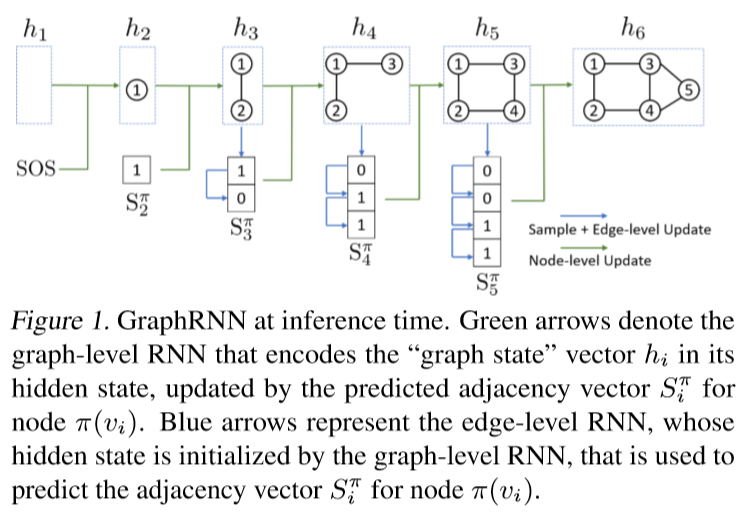
\includegraphics[width=.8\textwidth]{pics/GrpahRNN.png}
    \caption{GraphRNN生成图的过程}
    %\label{fig:my_label}
\end{figure}

GraphRNN模型是基于RNN的模型,以RNN为基础,从一个起始状态,利用RNN逐步生成图的状态,每一步向图中添加一个结点,再利用RNN生成新结点与已存在结点的连接关系,接着再向图中添加结点,重复下去直至EOS。结合之前的定义,$h_i$就是在生成过程中图的状态,它是对已经生成的图的一个encode之后的结果,每步输出$h_i$后就会将$h_i$作为另一个RNN的输入---用于生成边的连接关系的RNN。以上过程就是论文中提到的两个RNN---gaph-level RNN, edge-level RNN。
结合生成图的算法,我们可以知道有这几个部分是比较关键的:$f_{trans}, f_{out}, \mathcal{P}_{\theta_i}$。论文中对这部分都是采用神经网络来实现的,在我理解中$f_{tarns}$就是graph-level 的RNN,被$\theta_i$参数化的$\mathcal{P}_{\theta_i}$用于生成边的连接关系,即一个二进制序列。
有一个值得注意的点:$S^{\pi}_i$是一个不定长的序列,但是RNN的输入是定长的。论文中是这样处理的这个问题的:采用BFS遍历图,可以得到每个结点的依赖关系,通过对图数据集进行分析,可以得到每个节点依赖的已生成结点的数量$M$的分布,最终在训练时固定下M,即在训练时每个结点所依赖的结点数是确定的,$M$是个超参数。

\par 那么如何进行训练呢?(这部分论文中并没有进行详细的描述,代码中有较详细的过程)\\
首先要将传统格式的图数据转换为论文中定义的序列形式的图。


\par 看看这篇论文是否解决了一开始所提到的几个难点呢?
\begin{itemize}
    \item 生成空间太大且可变。个人理解论文中的graph-level和edge-level 的RNN相当于对图进行了编码,能否看作是对整个图的嵌入呢?
    \item 使用序列来表示图的生成过程,将一个确定的图的概率表示为联合概率$p(G, S^{\pi})$的边缘分布。
    \item 复杂的依赖关系。使用BFS遍历图,得到数据集中每个结点所依赖的结点的数量的分布,固定下来作为超参数。(\textbf{{\color{red}这是否可以作为一个改进的点呢?}})
\end{itemize}

\par 未来工作的方向。生成更大规模的图,高效地生成指定条件的图。


% \section{How powerful are graph neural networks?}
% 
论文地址:\href{https://arxiv.org/abs/1810.00826}{https://arxiv.org/abs/1810.00826}\\
GitHub地址:\href{https://github.com/weihua916/powerful-gnns}{powerful-gnns}

论文\cite{xu2018how}对以往的GNN模型的表现能力(区分能力)进行了理论上的分析,主要针对不同aggregation 的特点进行了分析,并针对以往的GNNs的弱点,设计了GIN(graph isomorphism network),达到了与WL sub tree相匹配的性能。论文中使用两种分类任务对以往的GNNs和GIN, WL sub tree 进行了测试:结点分类、图分类。

论文由一个问题开始讨论GNNs的区分能力。\\
给定两个图$G_1, G_2$,不同的GNNs可能会将它们(或者两图中的某两个结点)嵌入到相同的表示。这是为什么呢?这就要讨论GNNs是如何来获得结点/图的embeddings了。考虑一个通用的GNN模型:
$$
h_v^{(k)} = COMBINE(h_v^{(k-1)},  AGGREGATE({h_u^{(k-1)} | u \in \mathcal{N}_v } ) )
$$
上式中的$AGGREGATE$用来聚集邻居结点的信息(如mean, max, GRU, LSTM, GAT等),$COMBINE$则用来将聚集后的邻居结点的信息与结点自身的信息进行组合(如拼接。其实这很像一个图中的消息传播模型,现有的很多GNN模型也是基于消息传播的方法来汇聚邻居结点的信息,k层的GNN 相当与汇聚了来自k-hop的邻居的信息。({\color{red}{能否使用其他的框架来构建GNN模型呢?}})对于图$G$的embedding,是由$G$中的所有结点形成的(这涉及graph embedding的问题,参见其他论文)。
$$
h_G = READOUT(h_v^{(K)} | v \in G)
$$
再回到论文中的问题:\textbf{以往的GNN可能无法区分某些结点/图,即对不同的结点/图不能生成唯一的embeddin,不是injective的!}。根据结点/图的embedding生成的方法可以看出,关键在于$AGGREGATE, COMBINE, READOUT$,论文中将这些定义为 \textit{multi-set function},multi-set是一个可以有重复元素的集合,multi-set function就是定义在multi-set上的函数。问题就出在了GNNs使用的某些multi-set function上!
\par 论文主要对不同的AGGREGATE进行了分析,且主要分析了mean, max两种方法。
\begin{figure}
    \centering
    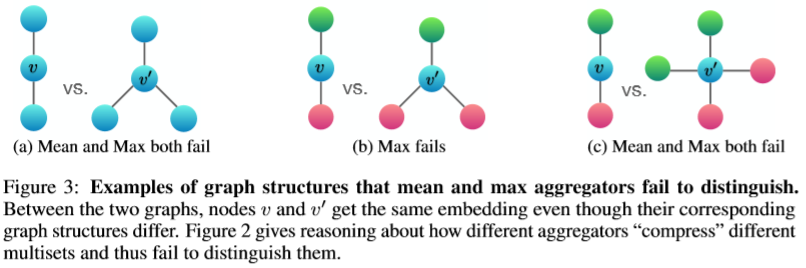
\includegraphics[width=1.\textwidth]{pics/mean-max.png}
    %\caption{Caption}
    %\label{fig:my_label}
\end{figure}
如上图所示,展示了mean, max 无法区分两个图中不同结点的邻居情况(neighborhood,即AGGREGATE后的结果是一样的)。论文中分别对mean, max的特性进行了阐述。\\
先给一个形式化的定义,假设$X$为某个结点的邻居结点集,$h(X)$就是AGGREGATE。
\paragraph{MEAN Learns Distributions} 当$h(X) = \frac{1}{|X|}\sum_{x\in X} f(x)$ 时,若对于不同的邻居结点集$X_1, X_2$,若$h(X_1) = h(X_2)$,则$X_1$和$X_2$有着相同的分布。从统计意义上来理解,相当于两个分布的均值(mean)相同。所以,当我们更需要捕捉图中某种信息的分布或者信息重复较少时,mean会有不错的效果。

\paragraph{MAX Identity "Skeleton"}(妙!) 当$h(X) = max_{x\in X}f(x)$时,若对于不同的$X_1, X_2$有$h(X_1) = h(X_2)$,则$X_1$和$X_2$有着相同的underlying set。当使用max作为AGGREGATE时,相当于对multi-set中的“重点”元素进行关注,当放在整个图中看时,相当于抽取了图中某种意义上比较“强”的结点。

\par 接下来就是重头戏 --- GIN了。
\par 论文中对结点和图的GIN定义如下:
$$
h_v^{(k)} = MLP^{(k)} ((1+\epsilon^{(k)} ) \cdot h_v^{(k-1)}+\sum_{u \in \mathcal{N}(v)} h_u^{(k-1)} ))  \newline
$$
$$
h_G = CONCAT(READOUT({h_v^{(k)} | v \in G}) | k = 0,1,...,K)
$$
看到上面的定义,你可能会疑惑,为什么GIN就比其他的GNNs好呢?这和以往的GNNs有什么区别呢?论文中对GIN使用的AGGREGATE进行了理论上的证明,证明GIN是injective的。
\par 论文中通过两个结论证明了GIN的injective性。说了几次injective了,那什么是injective呢?\\
\textbf{injective function}: 定义域中的每个不同的原像在值域中的像都是唯一的。
那么,为了让GNN有足够powerful的表现/识别能力,GNN需要尽可能精确地区分每个不同的结点/图(GNN作为以一种主要的embedding方法,高精度的表示能力能为下游任务打好基础),所以应尽量使AGGREGATE, COMMBINE, READOUT 是injective的。\\
{\color{red}证明GIN的injective}

\par 再来谈一下  Weisfeiler-Lehman (WL) graph isomorphism test 。WL isomorphism test 是用来比较两个图是否是同构的。先解释一下同构的概念。\\
抛开图同构,把同构概念单独拎出来看。对于两个系统中的对象,同构映射能够保持两个系统中的对象一一对应,且对象之间的关系也能够一一对应。图同构中,$v_1 = f(u_1), v_2 = f(u_2),u_1, u_2 \in G_1, v_1, v_2 \in G_2$,若$u_1, u_2$之间有边,则$(v_1, v_2) = g((u_1, u_2))$。\\
WL test 是通过迭代的聚集邻居的标签,每次迭代后将自己的标签和邻居们的标签映射成一个新的标签(相当于AGGREGATE后在COMBINE),迭代完成后比较两个图的标签分布(简单来说即各个标签分别有几个)是否一致({\color{red}结点的标签能否收敛呢?为什么标签的分布能用来判定是否同构呢?}),如果标签分布一致,则两个图可能是同构的。
WL subtree kernel\cite{shervashidze2011weisfeiler} 是基于 WL test的。我并没有通读论文,但是粗略看了一下图,感觉 WL subtree kernel和现在的GNN已经很像了, 对于每个结点,WL subtree kernel构建以该结点为root的树,子节点为其邻居结点,子节点的子节点是邻居结点,如此循环定义,最后以这颗树作为结点标签的依据。WL subtree kernel是目前基于聚合方式的GNNs的性能上界(证明见论文appendix)。但是WL subtree kernel并不能结合结点的信息,对于现在图中结点丰富的信息来说,这不免是有点浪费的,而且,个人认为WL subtree kernel捕捉的是图的结构(毕竟是衍生于图同构算法),或许图中的其他信息它是没有捕捉到的({\color{red}是什么信息呢?}) 

\par 关于未来的研究方向。有没有比基于聚集邻居结点信息(信息传递)方法更好的一个GNN框架呢?

关于WL test可参考的博客/非文献资料:
\begin{enumerate}
    \item \href{https://www.davidbieber.com/post/2019-05-10-weisfeiler-lehman-isomorphism-test/}{The Weisfeiler-Lehman Isomorphism Test}
\end{enumerate}

\part{Mathematics}
\section{chap01}
% 记录阅读文献时遇到的一些数学概念等
\subsection{采样}
采样是生成一堆数据的过程,如果最终生成的数据服从某个分布,则可以称这堆数据采样自这个分布。
\subsubsection{alias sampling }
一种高效的针对\textbf{离散概率分布}采样方法,但是要先经过预处理,预处理的时间为$O(n)$,但是与处理完成后采样的时间时$O(1)$。预处理的大致思路如下:\\
对于一个给定的离散概率分布:$p(X = x_i) , X = x_1, x_2, ..., x_n$。按照序号构造n个盒子,每个盒子按照顺序一一与$x_1, ..., x_n$对应,每个盒子的高度为$n \cdot p(X = x_i)$。接下来通过取长补短,把高度高于1的盒子切一部分分到其他高度低于1的盒子上,而且每个序号对应处不能有超过两个盒子。所以需要两个数组(Alias,Accept)来记录预处理的结果,一个用来记录每个序号除了原来的盒子还放了哪个盒子,一个用来记录每个序号的外来盒子有多高。\\
进行采样时,先决定使用哪个序号对应的盒子,再决定使用该序号内的原来的盒子还是外来的盒子。一个简单的例子Fig.\ref{fig:alias-sample}
\begin{figure}[h]
	\centering
	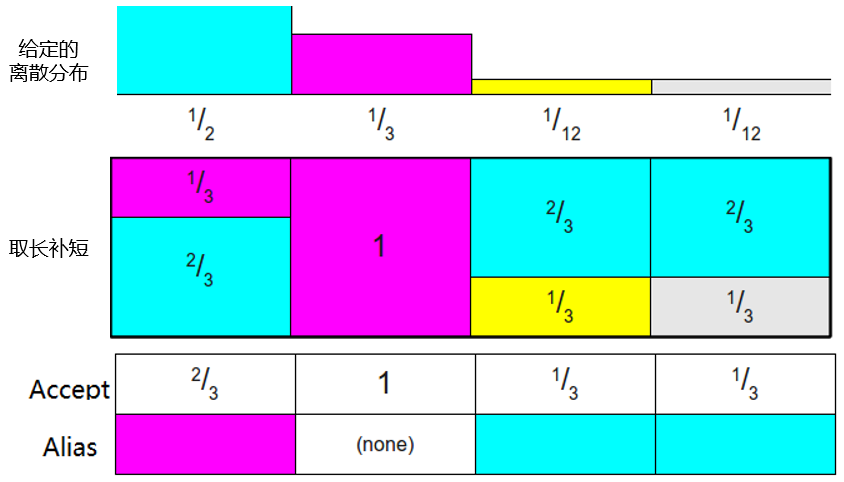
\includegraphics[width=.8\textwidth]{pics/alias-sample.png}
	\label{fig:alias-sample}
	\caption{Alias Sample例子}
\end{figure}


参考资料:
\begin{enumerate}
    \item \href{https://www.keithschwarz.com/darts-dice-coins/}{Darts, Dice, and Coins: Sampling from a Discrete Distribution}
    \item \href{https://www.cnblogs.com/dogecheng/p/13198198.html}{【图嵌入】DeepWalk 和 Node2Vec}
\end{enumerate}

\subsubsection{Importance Sampling}
重要性采样,一种近似的抽样方法, 通过一些数学上的变化, 使得可以对一些不好抽样的分布进行抽样和估计。这个会在强化学习中的off-policy的方法中用到, 从一个策略进行抽样, 更新另外一个策略。求函数$f(x)$的积分可以写成求期望的形式:
$$
E_{x \sim p(x)}[f(x)] = \int p(x) f(x) d x \approx \frac{1}{n} \sum_{i} f(x_{i})
$$
然而通常数据分布会比较复杂且积分也是一个复杂的过程,因此会用采样来代替之。上式中的第三项就是用采样来代替积分,其中$\frac{1}{n}$表示$p(x) = \frac{1}{n}$,即数据的分布。但是有时候$p(x)$是个很复杂的分布,从其重采样是很困难的,这个时候该怎么办呢?

找一个已易于采样的分布$q(x)$,如正态分布,从$q(x)$中采样得到的很多样本作为从$p(x)$中采样的样本集,那么问题就来了,这俩又不是同一个分布,$q(x)$中采样的样本集分布符合$p(x)$吗?先看一个公式:
$$
E_{x \sim p(x)}[f(x)] = \int q(x) \frac{p(x)}{q(x)} f(x) d x \approx \frac{1}{n} \sum_{i}  \frac{p(x)}{q(x)} f(x_{i})
$$
这个就是当我们从$q(x)$中采样代替$p(x)$后求$f(x)$积分/期望的公式。可以看出对于从$q(x)$中采样的样本赋予了不同的权重,因为样本集来自$p(x)$的概率是不一样的,其中重要性就是$\frac{p(x)}{q(x)}$。如Fig.\ref{fig:importance-sample}所示。注意:图中$p(z)$与$f(z)$的含义,$p(z)$是一种分布,是相对于$z$轴的采样点而言的,比如在红色的两个驼峰处,$z$的取点比较多,在其他地方$z$的取点就比较少,这叫样本分布服从$p(z)$。对于$f(z)$是一种映射关系,将$z$值映射到其他维度。

\begin{figure}[h]
	\centering
	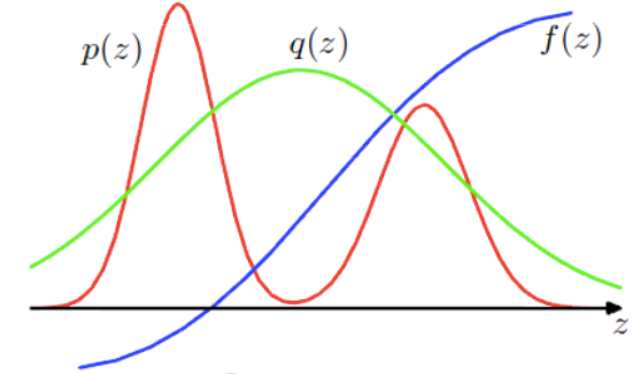
\includegraphics[width=.5\textwidth]{pics/importance-sample.png}
	\label{fig:importance-sample}
	\caption{重要性采样}
\end{figure}

参考:\href{https://www.jianshu.com/p/3d30070932a8}{随机模拟-Monte Carlo积分及采样(详述直接采样、接受-拒绝采样、重要性采样)}。


\subsubsection{接受-拒绝采样}
同样的问题:对于一个难以采样的分布$p(x)$,该怎么采样呢?选择一个易于采样的分布$q(x)$,从中采样,以一定的概率接受或拒绝采样到的样本,使得经过筛选后的样本集是服从$p(x)$的。
\begin{figure}[h]
	\centering
	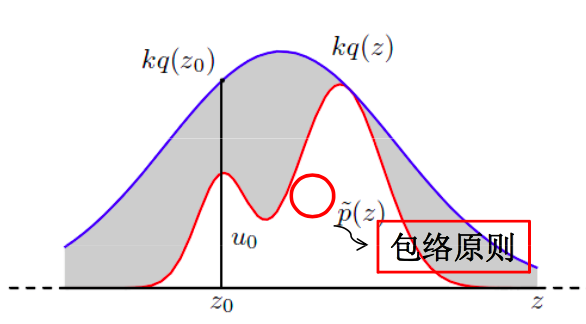
\includegraphics[width=.6\textwidth]{pics/accept-reject-sample.png}
	\label{fig:accept-reject-sample}
	\caption{接受-拒绝采样}
\end{figure}
具体该怎么操作呢?如Fig.\ref{fig:accept-reject-sample}所示,选择$q(x)$,乘以$k$得到$kq(x)$使之刚好能够保住$p(x)$。对于$q(x)$中采样到的样本$z_0$,从$[0, 1]$的均匀分布中取一个数$u_0$,如果$u_0 \le \frac{p(z_0)}{q(z_0)}$则接受$z_0$。

\subsection{eigen-value \& eigen—vector }
特征值,特征向量。
这两者到底有什么意义呢?


\subsection{Density estimation }

\subsection{MMD}
Maximum mean discrepancy。 用来衡量两个分布的差异。具体的衡量过程是:
假设有两个分布p, q,那么利用这两个分布分别生成两个样本集ps, qs,再假设有一个函数f,对于$pm = \sum_{i \in ps}f(i), qm = \sum_{j \in qs}f(j) $,
则分布p, q 在f上的MMD为 $pm$与$qm$的差或某种基于$pm, qm$ 的计算值。

\subsection{P, NP, NP-hard}
P问题:确定性计算机能够在指数级时间解决的问题;

NP问题:非确定性计算机能够在指数级时间解决的问题;

NPC问题:存在这样一个NP问题,所有NP问题都能约化成它,即只要解决了这个问题则所有NP问题都能解决。NPC需要满足两个条件:
\begin{itemize}
	\item 它是一个NP问题
	\item 所有的NP问题都能规约到它
\end{itemize}

NP-hard问题:满足NPC问题的第二个条件,但不一定满足第一条。NP-hard问题同样难以找到多项式时间的解法,但不一定是NP问题。这几者之间的包含关系如\ref{fig:P-NP-NPC-NP-hard}所示。

\begin{figure}[h]
	\centering
	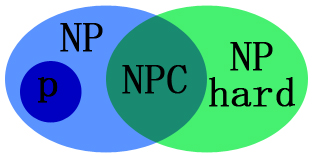
\includegraphics[width=.4\textwidth]{pics/P-NP-NPC-NP-hard.jpeg}
	\caption{P\_NP\_NPC\_NP-hard}
	\label{fig:P-NP-NPC-NP-hard}
\end{figure}



\subsection{傅里叶变换和小波分析}
傅里叶变换:知道一段时间内,信号的各个频率分量分别有多少。
小波变换:知道一段时间内,信号的各个频率分量分别有多少,以及它们都是什么时候出现的。

参考资料:\href{https://cseweb.ucsd.edu/~baden/Doc/wavelets/polikar_wavelets.pdf}{《The Wavelet Tutorial》}、\href{https://www.zhihu.com/question/22864189/answer/40772083}{如何通俗地讲解傅立叶分析和小波分析间的关系? - 咚懂咚懂咚的回答}。

\subsection{$l_1, l_2$范数对最优化问题的影响}
考虑以下优化问题:
\begin{equation}
	\begin{aligned}
		\min _{x \in \mathbb{R}^{n}} &\|x\|_{p}, \\
		\text { s.t. } & A x=b \label{eq-opt}
	\end{aligned}
\end{equation}
公式.\ref{eq-opt}中$p$表示0,1,2,$\|x\|_{p}$表示$x$的$l_p$范数。
在深度学习中,通常希望得到稀疏的解(稀疏的解,对数据的扰动也更鲁棒),即在满足约束的情况下,$x$中的非零值的数量尽可能多。咋一看,可能$l_0$范数是最符合情况的,但是$\|x\|_0$是不连续的,当$p=0$时,公式.\ref{eq-opt}就成了NP问题。当$A, b$满足一定条件时,$p=1$的时公式.\ref{eq-opt}的解也是$p=0$时的解。$l_1$范数优化问题更易求解。那么有没有更容易求解的范数呢,$l_2$可以吗?

对公式.\ref{eq-opt}进行转化:由于范数本身也是函数,该优化问题就可以视为在$A x = b$的约束下,$\|x\|_p$的最小值,从函数图像角度来看这个优化问题,就是\textbf{目标函数与约束函数的交集 --- 相交时的最小值}。

当$x \in \mathbb{R}^2$时,如Fig.\ref{fig:norm optimize}所示。
\begin{figure}[h]
	\centering
	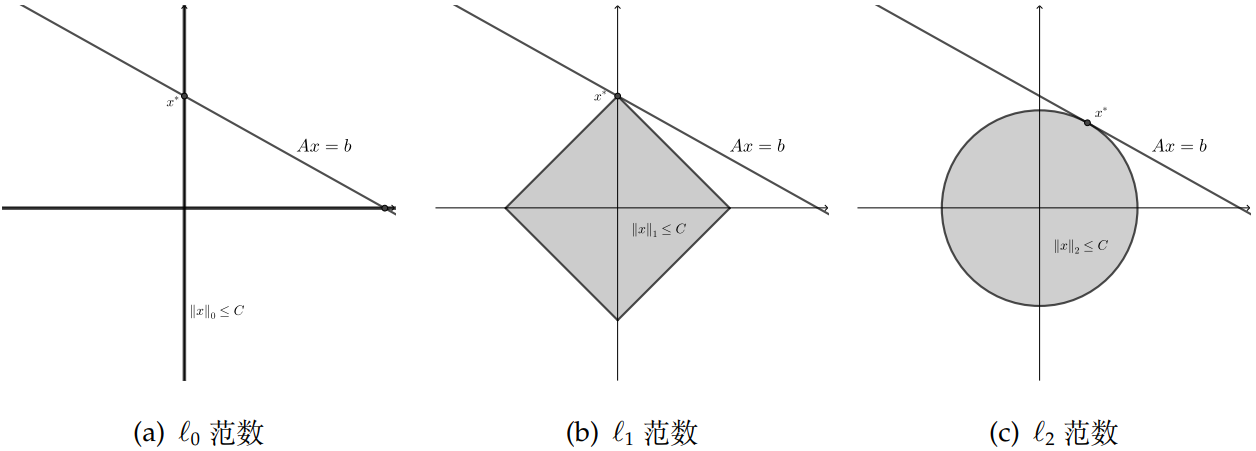
\includegraphics[width=.85\textwidth]{pics/norm optimize.png}
	\caption{$l_0, l_1, l_2$范数优化问题求解示意图}
	\label{fig:norm optimize}
\end{figure}
对$l_0$范数,$\{x | \|x\|_0 \leq 2\}$是全平面,它自然与$A x = b$相交;$\{x | \|x\|_0 \leq 1\}$退化成两条直线即坐标轴,此时问题的解就是$A x = b$与坐标轴的交点。
\begin{itemize}
	\item 对$l_1$范数,根据$C$不同,$\{x | \|x\|_1 \leq C\}$为一系列正方形,这些正方形的顶点落在坐标轴上,$A x = b$与这些正方形的交点一般是在正方形的顶点即相交于坐标轴,因此$l_1$范数的解有稀疏性
	\item 对$l_2$范数,根据$C$不同,$\{x | \|x\|_1 \leq C\}$为一系列圆,且圆有光滑的边界,圆和$A x = b$的交点可以是圆上任何一点,所以$l_2$范数优化问题一般不能保证解的稀疏性
	\item 对$l_2$范数,根据$C$不同,$\{x | \|x\|_1 \leq C\}$为一系列圆,且圆有光滑的边界,圆和$A x = b$的交点可以是圆上任何一点,所以$l_2$范数优化问题一般不能保证解的稀疏性
\end{itemize}

注意:\tbc{red}{这里目标函数与约束函数相交一般是指相切,$\{x | \|x\|_p \leq C\}$可以看成一个广义的球体,如果该球体与$A x = b$相交而不是相切,那么一定存在一个更小的$C'$使$\|x\|_p$更小且与$A x = b$相切,则$C'$成了比$C$更优的解,故一般考虑相切。}

参考资料:
\begin{itemize}
	\item《最优化:建模、算法与理论》,刘浩洋、户将、李勇锋、文再文编著,第一章,1.2
	\item \href{https://blog.csdn.net/red_stone1/article/details/80755144}{机器学习中 L1 和 L2 正则化的直观解释}
\end{itemize}


\subsection{Reparametrization}重参数化技术。参考:\href{https://spaces.ac.cn/archives/6705}{漫谈重参数:从正态分布到Gumbel Softmax}

\subsection{常用统计量}
\subsubsection{方差(Variance)} 一组数据的方差,描述的是数据与它们的均值的离散程度,衡量了这组数据的集中程度。方差可以分为样本方差和总体方差:
\begin{itemize}
	\item 样本方差:$S^2 = \frac{\sum_{i=1}^N(x_i - \bar{x})^2}{N-1}$,其中$\bar{x}$是\textbf{样本均值}
	\item 总体方差:$\sigma^2 = \frac{\sum_{i=1}^N(x_i - \mu)^2}{N}$,其中$\mu$是\textbf{总体均值}
\end{itemize}
\textbf{为什么不用要平方?}如果使用平均差($\frac{\sum_{i=1}^N |x_i - \bar{x}|}{N}$)来衡量一组数据的离散程度,可能不能很好的体现数据的分散程度(参考:\href{https://www.shuxuele.com/data/standard-deviation.html#WhySquare}{为什么要求差的平方?}),加上平方后可以放大偏离均值太远的数据的影响。也许这有点像注意力机制,在平均差中,$|x_i - \bar{x}|$的注意力值是$\frac{1}{N}$,在方差中,$|x_i - \bar{x}|$的注意力值是$\frac{|x_i - \bar{x}|}{N}$,这可以体现离均值越远的点对离散程度的贡献越大。

\subsubsection{标准差(Standard Deviation)} 标准差的平方就是方差,同理,标准差也可以分为样本std.和总总体std.:
\begin{itemize}
	\item 样本标准差:$S = \sqrt{S^2}$
	\item 总体标准差:$\sigma = \sqrt{\sigma^2}$
\end{itemize}

\subsubsection{T-statistic }


\subsubsection{p-value }

\subsubsection{t test、$\chi^2$检验}
$\chi^2$检验通常用于检验两个事件的独立性,例如可以用于分析自变量与因变量之间的独立性。如果$\chi^2$的值越大,则说明二者之间的关联性越大。

\subsection{数据的度量}
\subsubsection{定类变量}
即类别变量,其值域是某个离散的类别。能够对对象进行分类,能够判断对象之间是否同类或异类,如性别。\tbc{red}{不同类别之间没有大小关系}。

\textbf{【可以分类( $=$ 和 $\neq$),但不能排序】}

\subsubsection{定序变量}
定序变量的值不仅能够代表事物的分类,还能代表事物按某种特性的排序,但定序变量的值之间没有确切的间隔距离,\tbc{red}{只能排列出它们的顺序,而不能反映出不同值之间的距离},即不能反映一个值比另一个值大多少或小多少。如文化水平,其取值可以是文盲、小学、中学、大学等,值之间有顺序关系(如大学 $\textgreater$ 小学),但不能反映不同文化程度之间的距离。

\textbf{【可以分类( $=$ 和 $\neq$),可以排序($\textgreater$ 和 $\textless$),但不能($+$ 和 $-$ )】}

\subsubsection{定距变量}
定距变量的值之间\tbc{red}{可以比较大小,两个值的差有实际意义}。能确切测量值之间的高低、大小次序之间的距离,因而具有加与减的数学特质。但是,\tbc{red}{定距变量没有一个绝对的零点},不能乘除或倍数的形式来说明它们之间的关系。例如华氏温度:10、20、30,30比20高10,但华氏度30不是10的三倍热(\tbc{red}{0不是没有温度})。

\textbf{【可以分类( $=$和 $\neq$ ),可以排序($\textgreater$ 和 $\textless$),可以($+$ 和 $-$ ),但不能($\times$和 $\div$ )】}

\subsubsection{定比变量}
定比变量除了具有定距变量的特性外,还具有一个真正的零点,因而它具有乘与除(×、÷)的数学特质。如A的体重是60kg,而B的体重是30kg,可以算出前者是后者的两倍重,因为其零点是绝对的。

\textbf{【可以分类( $=$和 $\neq$ ),可以排序($\textgreater$ 和 $\textless$),可以($+$ 和 $-$ ),可以($\times$和 $\div$ )】}

以上四种变量类型的性质是逐渐继承的。

参考:\href{https://blog.csdn.net/YYIverson/article/details/100068865}{【统计学】区分定类、定序、定距、定比变量!!}。

\subsection{拉格朗日对偶性}
约束最优化中常用的一种方法。利用拉格朗日对偶性(Lagrange duality)将原始问题转换为对偶问题,通过求解对偶问题得到原始问题的解。

\subsubsection{原始问题}假设$f(x), g_i(x), h_j(x)$是定义在$\mathbb{R}^n$的连续可微函数。原始最优化问题为:
\begin{align}
	\mathop{min}_{x \in \mathbb{R}^n}&\quad f(x) \nonumber \\
	s.t.&\quad g_i(x) \leqslant 0, i = 1, 2, ..., k \nonumber \\
		&\quad h_j(x) = 0, j = 1, 2, ..., l \nonumber
\end{align}

引进广义朗格朗日函数:
$$
L(x, \alpha, \beta) = f(x) + \sum_{i=1}^k a_i g_i(x) + \sum_{i=j}^l \beta_j h_j(x)
$$
其中,$x \in \mathbb{R}^n$,$\alpha, \beta$是拉格朗日乘子,$\alpha_i \geqslant 0$。将$L$看作$\alpha, \beta$的函数(固定$x$),求其最大值,即:
$$
\mathop{max}_{\alpha, \beta:\alpha_i \geqslant 0} L(x, \alpha, \beta)
$$
注意,$\mathop{max}_{\alpha, \beta:\alpha_i \geqslant 0} L(x, \alpha, \beta)$表示固定$x$,$\alpha, \beta$作为变量来使$L$最大化,此时再固定$\alpha, \beta$即可得到一个关于$x$的函数:
$$
\theta_P (x) = \mathop{max}_{\alpha, \beta:\alpha_i \geqslant 0} L(x, \alpha, \beta)
$$
$P$表示原始问题。分析一下$\theta_P$:
\begin{myitemize}
	\item 当$x$违反原始约束$g_i(x) > 0$或$h_j(x) \neq 0$,则可以很容易调整对应的$\alpha_i, \beta_j$使$\theta_P(x)$取得$+\infty$。(\textbf{$\alpha_i \geqslant 0$的原因})
	\item 当$x$满足原始约束时,则有:
	$$
	\theta_P(x) = \mathop{max}_{\alpha, \beta:\alpha_i \geqslant 0} L(x, \alpha, \beta) = f(x)
	$$
	考虑$f(x) + \sum_{i=1}^k a_i g_i(x) + \sum_{i=j}^l \beta_j h_j(x)$,对于任意$x$(即固定$x$),显然有$h_j(x) = 0$,且$g_i(x) \leqslant 0$,则$\mathop{max}_{\alpha, \beta:\alpha_i \geqslant 0} L(x, \alpha, \beta)$\textbf{肯定有$\alpha_i = 0$},所以,
	$$
	\mathop{max}_{\alpha, \beta:\alpha_i \geqslant 0} L(x, \alpha, \beta) = f(x) + \sum_{i=1}^k 0 \cdot g_i(x) + \sum_{i=j}^l \beta_j h_j(x)
	$$
	即$\theta_P(x) = \mathop{max}_{\alpha, \beta:\alpha_i \geqslant 0} L(x, \alpha, \beta) = f(x)$
\end{myitemize}
因此,
$$
\theta_P(z)= \begin{cases}f(x), & x\ satisfies\ subjects \\ +\infty, & \text { otherwise }\end{cases}
$$
所以$\theta_P(x)$的极小就等价于原始问题的解,即:
$$
\mathop{min}_{x} \theta_P(x) = \mathop{min}_{x} \mathop{max}_{\alpha, \beta: \alpha_i \geqslant 0} L(x, \alpha, \beta)
$$
因此,原始不等式约束优化问题转化成了广义\textbf{拉格朗日的极小极大问题},定义原始问题的最优值:
$$
p^* = \mathop{min}_{x} \theta_P(x)
$$

\subsubsection{对偶问题}
定义关于$\alpha, \beta$的函数,
$$
\theta_D(\alpha, \beta) = \mathop{min}_{x} L(x, \alpha, \beta)
$$
$D$表示其为对偶问题,其含义可与$\theta_P$类别。考虑$\theta_D$的极大化,即:
$$
\mathop{max}_{\alpha, \beta: \alpha_i \geqslant 0} \theta_D(\alpha, \beta) = \mathop{max}_{\alpha, \beta: \alpha_i \geqslant 0} \mathop{min}_{x} L(x, \alpha, \beta)
$$
$\mathop{max}_{\alpha, \beta: \alpha_i \geqslant 0} \mathop{min}_{x} L(x, \alpha, \beta)$称为\textbf{拉格朗日函数的极大极小问题}。将朗格朗日的极大极小问题转化为优化问题:
\begin{align}
	\mathop{max}_{\alpha, \beta} \theta_D(\alpha, \beta)&\quad = \mathop{max}_{\alpha, \beta: \alpha_i \geqslant 0} \mathop{min}_{x} L(x, \alpha, \beta) \nonumber \\
	s.t.&\quad \alpha_i \geqslant 0, i = 1, 2, ..., k \nonumber
\end{align}
该问题称为原始问题的对偶问题,定义对偶问题的最优值:
$$
d^* = \mathop{max}_{\alpha, \beta: \alpha_i \geqslant 0} \theta_D(\alpha, \beta)
$$

\subsubsection{原始问题与对偶问题的关系}
若原始问题和对偶问题都有最优值,那么二者的最优值有如下关系:
$$
d^* = \mathop{max}_{\alpha, \beta: \alpha_i \geqslant 0} \mathop{min}_{x} L(x, \alpha, \beta) \leqslant \mathop{min}_{x} \mathop{max}_{\alpha, \beta: \alpha_i \geqslant 0} L(x, \alpha, \beta) = p^*
$$
\textbf{证明:}
\begin{quotation}
	$$
	\theta_D(\alpha, \beta) = \mathop{min}_{x} L(x, \alpha, \beta) \leqslant L(x, \alpha, \beta) \leqslant \mathop{max}_{\alpha, \beta: \alpha_i \geqslant 0} L(x, \alpha, \beta) = \theta_P(x)
	$$
	即,
	$$
	\theta_D (\alpha, \beta) \leqslant \theta_P (x)
	$$
	即,
	$$
	\mathop{max}_{\alpha, \beta:\alpha_i \geqslant 0} \theta_D (\alpha, \beta) \leqslant \mathop{min}_{x} \theta_P (x)
	$$
	得证。
\end{quotation}
\textbf{推论:}
\begin{quotation}
	若$x^*, (\alpha^*, \beta^*)$分别是原始问题和对偶问题的\textbf{可行解},若$d^* = p^*$,则$x^*, (\alpha^*, \beta^*)$分别是原始问题和对偶问题的\textbf{最优解}。
\end{quotation} 
那什么样的条件才满足$d^* = p^*$呢?

\textbf{Karush-Kuhu-Tucker(KKT) 条件}\label{kkt}
\begin{quotation}
	对原始问题和对偶问题,假设$f(x), g_i(x)$是凸函数,$h_j(x)$是仿射函数,并且不等式约束$g_i(x) \leq 0$是\textbf{严格可行的},即存在$x$,对所有$i$有$g_i(x) < 0$。则$x^*, (\alpha^*, \beta^*)$分别是原始问题和对偶问题的解的充要条件是$x^*, (\alpha^*, \beta^*)$满足以下KKT条件:
	\begin{align}\nonumber
		\nabla_x L(x^*, \alpha^*, \beta^*) &= 0 \nonumber \\
		\alpha_i^* g_i(x^*) &= 0, i = 1, 2, ..., k \nonumber \\
		g_i(x^*) &\leq 0, i = 1, 2, ..., k \nonumber \\
		\alpha_i^* &\geq 0, i = 1, 2, ..., k \nonumber \\ 
		h_j(x^*) &= 0, i = 1, 2, ..., l \nonumber 
	\end{align}
	
\end{quotation}

\subsection{Sequence Minimal Optimization(SMO)}\label{smo}
序列最小最优化算法,SMO是一种启发式算法,通常用于求解凸二次规划问题。

\subsection{正定核}\label{pdkf}
Positive definite kernel function。一个核函数为正定核的充要条件:
\begin{quotation}
	对任意$x_i \in \mathcal{R}, i = 1, 2, ..., m$ ,$\kappa(x_i, x_j)$对应的Gram矩阵 $[\kappa(x_i, x_j)]_{m \times m}$是半正定矩阵。
\end{quotation}

\subsubsection{常用核函数}
\begin{itemize}
	\item 多项式核:$\kappa(x, z) = (x \cdot z + 1)^p$
	\item 高斯核:$\kappa(x, z) = e^{- \frac{||x - z||^2}{2 \sigma^2}}$。为啥说高斯核等于无穷维呢?因为 $e^x$ 这个函数进行展开的话有无穷维。
\end{itemize}


\subsection{机器学习中常见的数据分布}
这里将介绍常见的一些分布,主要通过这些分布的密度函数、分布函数来介绍,以及其在机器学习/深度学习中的一些体现和应用。
\subsubsection{Gaussian}高斯分布,正态分布,钟形分布。
$$
f(x) = \frac{1}{\sqrt{2 \pi} \sigma} e^{- \frac{(x - \mu)^2 }{2 \sigma^2}}
$$
正态分布的两个参数为:$\mu, \sigma$,分别表示正态分布的均值和标准差。标准正态分布即 $\mu = 0, \sigma = 1$ 的正态分布。

\subsubsection{Laplace}拉普拉斯分布。
$$
f(x) = \frac{1}{2b} e^{- \frac{{|x - \mu|}}{b}}
$$


\subsection{变量之间的相关性检验}
在进行数据分析的时候,如果要对自变量与因变量之间的关系进行分析,或者说在多任务学习中,分析不同任务之间的相关性时,如何检验这种相关性是很重要的。

\subsubsection{Person 相关系数}
即皮尔逊相关系数,反应两个变量相似性的统计量,衡量的是两个变量之间的线性相关性,变化的趋势。定义变量 $X, Y$ 的 Person 系数为:
$$
\rho_{X, Y}=\frac{\operatorname{cov}(X, Y)}{\sigma_{X} \sigma_{Y}}=\frac{E[(X-E X)(Y-E Y)]}{\sigma_{X} \sigma_{Y}}=\frac{E(X Y)-E(X) E(Y)}{\sqrt{E\left(X^{2}\right)-E^{2}(X)} \sqrt{E\left(Y^{2}\right)-E^{2}(Y)}}
$$
其中 $\sigma$ 表示方差。皮尔逊相关系数通常衡量的是两个实值变量之间的相关性,$\rho_{X, T} \in [-1, 1]$,小于 0 表示负相关,大于 0 表示正相关,0 则表示二者不具备\textbf{线性}相关性。注意,不相关不等于独立。当 $X, Y$ 是均值为 0 的变量时,则有:
$$
\rho_{X, Y}=\frac{E(X Y)}{\sqrt{E\left(X^{2}\right)} \sqrt{E\left(Y^{2}\right)}}=\frac{\frac{1}{N} \sum_{i=1}^{N} X_{i} Y_{i}}{\sqrt{\frac{1}{N} \sum_{i=1}^{N} X_{i}^{2}} \sqrt{\frac{1}{N} \sum_{i=1}^{N} Y_{i}^{2}}}=\frac{\sum_{i=1}^{N} X_{i} Y_{i}}{\sqrt{\sum_{i=1}^{N} X_{i}^{2}} \sqrt{\sum_{i=1}^{N} Y_{i}^{2}}}=\frac{\sum_{i=1}^{N} X_{i} Y_{i}}{\|X \mid\| Y \|}
$$
显然,此时皮尔逊相关系数就成了两个向量的 $cosine$函数,即余弦相似度,再进一步,如果 $X, Y$ 的模长为 1,则皮尔徐相关系数 $\rho_{X, Y} = X \cdot Y$,即成了向量的内积。所以,其实我们也可以反推出来,向量的内积其实衡量的是向量的一种相似度,一种未归一化的相似度。

皮尔逊相关系数可以用来衡量两个用户之间的相似性,例如以两个用户对物品的评分向量计算皮尔逊相关系数。

\textbf{缺点}:
\begin{itemize}
	\item 从皮尔逊相关系数的公式可以看出,如果两个变量的配对的数据(即 $X, Y$ 都有值的数据,在评分矩阵中体现为两个用户对同一个物品进行了评分你)很少时,均值和方差的估计是不太准确的,且只有一个配对时是无法计算皮尔逊相关系数的(因为方差为 0);
	\item 没有两个变量的配对的数目的影响,即可能 $X, Y$ 之间的配对数量很大,且值也比较接近,但是如果 $X, Z$ 配对数量很小但评分基本一样,则可能 $X, Y$ 的皮尔逊相关性会小于 $X, Z$ 的相关性,这显然是不合理的;
	\item 要求变量的方差为 0,即要求变量的值是取自一个方差不为零的分布(通常假设其来自正态分布),其实从用户评分角度来看,即要求用户的偏好是可以区分的;
	\item 对绝对值不敏感,即 $X, Y$ 的趋势相似,且值的分布也比较相似,$X, Z$ 的趋势相似但 $X$ 的平均值很大,$Z$ 的平均值很小,用皮尔逊相系数衡量的话,可能 $X, Z$ 之间更相似。在推荐中,可能优的用户习惯给低分,有的用户习惯给高分; 
\end{itemize}

\subsubsection{Spearman 秩相关系数}
Spearman 秩相关系数是一种无参数(与分布无关)检验方法,用于度量变量之间联系的强弱。在没有重复数据的情况下,如果一个变量是另外一个变量的严格单调函数,则Spearman秩相关系数就是 +1 或 -1,称变量完全 Spearman 秩相关。注意这和 Pearson 完全相关的区别,只有当两变量存在线性关系时,Pearson 相关系数才为 +1 或 -1。

将 $X, Y$ 两个变量的取值看作序列,计算 $x_i$ 在 $X$ 中的顺序(秩),对于 $Y$ 计算相同的值,对于一对 $(x_i, y_i)$ 而言,秩差 $d_i$ 为 $x_i, y_i$ 的秩的差,则斯皮尔曼系数为:
$$
\rho_{s} = 1 - \frac{6 \sum_{i=1}^N d_i^2}{N(N^2 - 1)}
$$
显然,斯皮尔曼系数不仅可以度量变量之间的线性和非线性相关性,如 $y = x^2, x > 0$,用皮尔逊系数度量则为不相关的,但是在斯皮尔曼系数下可以算得二者得相关性是 1。其实,虽然斯皮尔曼不要求变量是来自某个分布得,但是可以看出它还是要求变量得值是可以比较得,否则秩就没有意义了。且要处理变量中存在重复值得情况,即在 $X$ 或 $Y$ 中存在重复值时该如何赋予秩。

当然,对于不同的变量类型,有不同得检验方法,具体可以参见:\href{https://zhuanlan.zhihu.com/p/396580986}{相关分析最全总结}、\href{https://zhuanlan.zhihu.com/p/94070722}{要做相关性分析,该如何选择正确的统计方法?}。

\subsection{Jacobean Hessian}

\subsection{指数移动平均}
指数移动平均在深度学习的梯度下降优化算法中出现的频率很高。


\clearpage
\part{Machine Learning}
{\noindent}	 \rule[-10pt]{17.5cm}{0.5em}\\  %{\noindent} 表示取消缩进, \rule[水平高度]{长度}{粗细}
\section{Basics}
% 用于记录一些常见的机器学习, 深度学习的概念

\subsection{L1/2 regularization}
$L1, L2$ 正则即在优化函数的基础上加上参数的 $L1, L2$ 范数, 即 $L1(\boldsymbol{w}) = \sum_{i=1}^{n} |w_i|$, $L2(\boldsymbol{w}) = \sum_{i=1}^{n} w^2$. 这里从梯度的角度阐述一下二者的区别, 这里仅求范数对参数的导数, 并省略了一些常数. 

$L1$: 
$$
\begin{aligned}
	\frac{\partial L1}{\partial w_i} &=  \text{sign}(w_i) \\
	w_i &= w_i - \eta\ \text{sign}(w_i)	
\end{aligned}
$$

$L2$: 

$$
\begin{aligned}
	\frac{\partial L2}{\partial w_i} &=  w_i \\
	w_i &= w_i - \eta\ w_i
\end{aligned}
$$
通过上述参数更新方式的对比, 可以很明显地看到 $L1$ 约束更新参数时只与参数地符号有关, 因此, 当 $w_i \in [1, +\inf)$ 时, $L2$ 能够更快地减小参数, 而当 $w_i \in (0, 1)$ 时, $L1$ 能更快地减小参数, 更容易使参数接近 0, 即小于 1 地参数有更大概率接近 0. 

当然, 除了从梯度的角度解释, 还可以从优化的角度和概率的角度. $L1$ 假设参数服从 Laplace 分布, 而 $L2$ 假设参数服从 Gaussian 分布, 从这两个分布 (标准的 Laplace 分布和标准的 Gaussian 分布) 的形状也可以看出 $L1$ 正则化下的参数有更大的概率接近或等于 0. 

\subsubsection{L1/2 的先验分布}
机器学习通常是在给定观察到的数据后对模型的参数进行估计, 相当于求后验概率: 
$$
MAP = \log P(y | X, w) P(w) = \log P(y | X, w) + \log P(w)
$$
即后验概率为似然函数加上参数的先验. 若假设 $w$ 的先验服从 0 均值的正态分布, 则: 
$$
\log P(w) = \log \prod_{j} P(w_j) = \log \prod_{j} \frac{1}{\sqrt{2 \pi } \sigma} e ^ {-\frac{w_j^2}{2 \sigma^2}} =-\frac{1}{2 \sigma^2} \sum_j w_j^2 + C
$$
可以看到, 在高斯分布下 $\log P(w)$ 的效果等价于在代价函数中增加了 L2 正则项. 若 $w$ 服从均值为 0, 参数为 $a$ 的拉普拉斯分布, 则: 
$$
\log P(w) = \log \prod_{j} P(w_j) = \log \prod_{j} \frac{1}{\sqrt{2 a} \sigma} e^{-\frac{|w_j|}{a}} = -\frac{1}{2a} \sum_j |w_j| + C
$$
可以看到, 在拉普拉斯分布下 $\log P(w)$ 等价于在代价函数中增加了 L1 正则项. 

\begin{flushright}
	
\end{flushright}参考: \href{https://www.zhihu.com/question/37096933/answer/475278057}{l1 相比于 l2 为什么容易获得稀疏解? - ser jamie的回答}. 


\subsection{判别模型、生成模型}
\begin{itemize}
	\item 判别模型: 直接对判别函数或者条件概率分布函数进行建模, 不考虑样本的产生模型, 直接研究预测模型
	\item 生成模型: 学习联合概率密度$P(Y, X)$, 然后求出条件概率分布$P(Y|X) = \frac{P(X, Y)}{P(X)}$, 不仅要求出联合分布, 还要求出训练数据的分布$P(X)$ ({\color{red}{不一定要计算$p(X)$, 因为对于同一个样本, 计算它属于不同分类时, 其$p(X)$是一样的, 对判别没有帮助}}) . 生成模型表示了输入$X$产生输出$Y$的生成关系
\end{itemize}

对于生成式模型, 可以这样理解: \\
$p(x | y) = p(y)p(x | y)$表示的是, 从$p(y)$中采样一个$y$, 然后根据$p(x|y)$采样一个$x$. 生成式模型希望找到那个能够使$p(x, y)$最大的$y$. 1


生成模型从统计的角度表示数据的分布情况. 判别模型不能反映训练数据本身的特性, 但它不断寻找不同类别之间的最优分类面. 

也可以从 \textbf{决策函数$Y=f(X)$或条件概率分布$P(Y|X)$} 的角度来看待判别模型和生成模型: 
从数据中学习一个分类器时, 希望通过给定的输入$X$输出相应的$Y$. 这个模型的一般形式为: 
\begin{itemize}
	\item 决策函数$Y=f(X)$: 输入一个$X$就输出一个$Y$, 可以将$Y$于阈值比较得到$X$的类别
	\item 条件概率分布$P(Y|X)$: 输入一个$X$, 输出$X$属于各个类的概率, 如$P(c_1 | X), P(c_2 | X)$. 取其中最大的作为$X$的类别
\end{itemize}
实际上$P(Y|X)$是隐含了或者说可以转化为决策函数形式$Y=f(X)$的. 例如, 将条件概率分布改写为$Y = \frac{P(c_1 | X)}{P(c_2 | X) }$. 

参考资料: \href{https://blog.csdn.net/fishmemory/article/details/51711114}{判别模型(Discriminative model)和生成模型(Generative model)}、\href{https://developers.google.cn/machine-learning/gan/generative?hl=zh-cn}{Background: What is a Generative Model?}. 

\subsection{熵、相对熵、交叉熵、互信息} 
\textbf{\checkmark 2020-10-08}\\
这些概念来自信息论\cite{6773024}. 简单来说, 熵指的是不确定性或者信息量, 熵越大不确定越大. 相对熵也叫KL(Kullback-Leibler divergence)散度, 用来比较两个概率分布之间的差异. 不论是熵、相对熵、交叉熵, 都可以看作针对某个 (或多个) 随机变量, 对该随机变量的概率分布的一个某种熵 (熵、相对熵、交叉熵) 的计算. 接下来就从数学上来对其进行描述. 

\textbf{熵}: 先介绍自信息的概念. 对于某个随机变量$X$, 当$X$取值为$x_0$时的自信息为$I(x_0) = -log\ p(x_0)$, 即事件$x_0$发生时所带来的信息量, 如果一个事件发生的概率越大, 则其带来的信息量越小. 熵是自信息的均值. 即$X$取任一值时所能带来的期望信息量, 故$X$的信息熵$H(X) = -E_{x\sim p}I(x)$ (其中p是$X$所服从的分布) , 即$H(X) = -\sum_{x \in X}log\ p(x)$. \textbf{因为随机变量$X$会服从某个分布, 假设是$p$, 则$H(X)$也可以看作是概率分布$p$的信息量的期望. }

\textbf{相对熵}: 也称作KL散度. KL是在信息熵的基础上定义的, 用来衡量两个分布的差异, 其实由上述熵的含义可知, 其实KL也可以看作是随机变量$X$, 其可能服从的两个分布之间的差异. 假设可能服从的两个分布分别是$p, q$, 则以$q$去接近$p$时的KL散度表示为: $D_{KL}(p||q) = \sum_{x \in X} p(x) log\ \frac{p(x)}{q(x)} = E_{x\sim p} log\ \frac{p(x)}{q(x)}$. 经过化简可得$D_{KL} = -H(p) - \sum_{x \in X}p(x)log\ q(x)$. 

\textbf{交叉熵}: \label{ce}cross-entropy, 与KL散度相似, 也是用来衡量随机变量$X$可能服从的两个分布$p, q$之间的差异的. 其数学上的定义为: $Cross-Entropy(p, q) = -E_{x\sim p} log\ q(x) = - \sum_{x \in X}p(x)log\ q(x)$. 很显然, 交叉熵比KL散度多了一个$H(p)$, 即$Cross-Entropy(p, q) = D_{kL}(p || q) + H(p)$. 

机器学习中常使用交叉熵, 既然KL散度和交叉熵都可以达到相同的目的, 那为什么不使用KL散度呢?在机器学习中, 上述的分布$p$常作为数据的真实分布, 而$q$作为数据的预测分布, 此时$H(P)$则可以视作一个常数 (因为给定数据后, 其真实分布是确定的), 在优化模型的参数时, $H(P)$并不会对参数的优化做出贡献 (不会影响优化过程) , 故使用交叉熵即可. 

\subsection{关于交叉熵损失函数的一点理解}
交叉熵损失函数可以从多个角度进行理解. 从概率论的角度, 在极大似然概率估计中, 希望参数能够使得已有样本出现的概率最大. 

\paragraph{二分类}
在分类任务中, 由于不同样本是有标签的, 样本出现的概率应该与标签对应, 例如p表示1样本出现的概率, 则1-p表示0样本出现的概率, 那么对于1样本极大化的应该是p, 对于0样本极大化的应该是1-p. 

样本的极大化后的概率取对数后为相加的形式. 则对于一个样本, 其极大化的表示可以写成$log p$  (1样本) , 或者$log(1-p)$ ( 0样本) . 如果用一个统一的式子表示的话, 可以写成$y log p + (1-y) log(1-p)$, 其中y取0或1. 

通常是对损失函数最小化, 所以可以在极大化的表示前加个符号就变成了交叉熵损失函数: $- y log p - (1-y) log(1-p)$. 将一个batch里的样本的损失累加起来就是常见的形式了. 并且, 在用模型计算p时, p通常通过一个函数来表示$f(x)$, x即为输入的样本, $f(x)$可以是各种机器学习模型, 如逻辑回归、神经网络等. 


\paragraph{多分类}
对于一个$C$个类别的多分类任务, 用$p_i$表示样本$x$被预测为第$i$类的概率, $x$的真实类被为$c$, 也可以用一个one-hot向量$y = [y_1, y_2, ..., y_C],\ y_i = 1\ if\ i = c\ else\ y = 0$表示$x$的真实类别. 那么$x$的损失即可表示为$loss_x = \sum_{i=1}^C y_i\ \log p_i$. 显然, $loss_x = \log p_c$. 通常, 如果$\{p_i\}_{i=1}^C$是未归一化的, 那么实践中, $loss_x = \log \frac{e^{p_c}}{\sum_{i=1}^C e^{p_i}}$

除了从极大似然的角度来理解交叉熵损失函数, 当然也可以直接从交叉熵\ref{ce}的角度来理解. 

\subsection{方差与偏差}
\paragraph{偏差 (Bias) }通常是指: 对于一种模型, 它的平均 (训练多次也就得到了多个模型实例) 预测结果与真实值之间的差距. 偏差度量的是学习到的函数与真实函数的差距的期望, 即$E[\hat{f} - f]$. 

\paragraph{方差 (Variance) }选用一种模型 (如KNN, SVM, NN等) , 使用不同的数据集可以得到该种模型的多个实例 (即训练好参数的模型) . \textbf{这些模型}对于同一个输入给出的预测值的方差, 即$E[(\hat{f} - E[\hat{f}])^2]$. 方差是受所使用的训练集影响的, 我们使用不同分布的数据集训练出来的模型会导致学出来的模型参数变化, 这反映出来的就是针对同样的输入会产生不一样的预测值, 这些预测值的方差就反映了模型的方差. 

在模型很复杂的时候, 在训练集上学习的模型能够准确地预测, 产生较小的偏差, 但是更容易产生大方差, 因为模型有更多的参数, 能够“死记硬背”记下输入与输出的映射关系, 这个时候模型可能记住了一些没用的东西甚至是噪声, 而模型是没有见过测试集的, 稍微有些不同的数据点的输出可能会有较大的差别, 从而产生大的偏差.  --- \textbf{过拟合}

当模型较简单的时候, 可能无法充分地利用训练集, 在测试集上会产生较大的偏差, 但是因为模型参数少, 模型关注地特征较少, 光从这些特征来看的话, 测试集中的数据与训练集中的数据会有更高的相似性, 因此就算不同的数据输入, 但是由于某些特征被忽略后数据反而是相似的, 所以模型给出的输出是类似的, 因而方差小. --- \textbf{欠拟合}

参考: \href{http://scott.fortmann-roe.com/docs/BiasVariance.html}{Understanding the Bias-Variance Tradeoff}, \href{http://www.r2d3.us/visual-intro-to-machine-learning-part-2/}{Model Tuning and
	the Bias-Variance Tradeoff} (可视化解释, 墙裂推荐) , \href{https://www.cnblogs.com/makefile/p/bias-var.html}{偏差方差分解} (分解过程的详细推导) . 


\textbf{注意: }\textbf{一种模型相当于一个函数空间}, 当我们选择一种模型进行训练, 得到了该种模型的各个参数, 就相当于得到了一个实例化的模型. 模型种类相当于类, 训练好的模型相当于对象. 喂数据训练模型时相当于在某个特定的函数空间中找到一个合适的函数 --- 即我们要的模型. 有时候训练后的模型效果不好, 可能不是这种模型不行, 可能是没有在这个函数空间中找到合适的函数. 

\subsection{交叉验证}
在训练模型的时候, 通过会把数据集划分为训练集和测试集, 测试集的作用用于学习模型参数, 测试集是为了检验模型在未见过的数据上的效果. 但是只将数据集划分为测试集和训练集有以下问题: 
\begin{itemize}
	\item 最终模型与参数的选取将极大程度依赖于你对训练集和测试集的划分方法. 不同的划分情况, 学习出来的参数是不一样的; 固定模型参数, 模型在不同划分上的表现也是不一样的. 这种情况使得我们无法准确对模型的能力进行评估, 不利于我们选择最优的模型 (指何种模型) 以及最优的模型参数 (一般是指超参数, 而不是模型学习到的参数) ; 
	\item 该方法只用了部分数据进行模型的训练, 无法充分利用已有的数据. 测试的效果只是针对某个划分, 并不是针对整个数据集, 不够有说服力; 
\end{itemize}
为了解决以上为题, 即1) 选择最好的模型与参数; 2) 充分利用数据, 使模型的测试结果有说服力, 就有了交叉验证 (Cross Validation) . 常见的交叉验证方法: 
\begin{itemize}
	\item LOOCV (Leave-one-out cross-validation) , 即留一验证. 对于有N个样本的数据集, 重复N次, 每次选择其中一个作为测试集, 其他的作为训练集, 这样就得到了N个$(train_i, test_i), i = 1, ..., N$训练集、测试集对儿. 分别用这N个训练集-测试集对儿来训练模型, 这样就可以学习到N个模型. 每个模型都可以得到一个测试得分, 进行平均后就作为这类模型在这个数据集上的测试分数
	
	\item K-fold CV, 即K折交叉验证. 与LOOCV类似, 但是对数据集的划分不同, 是把数据集划分为K份, 每次取其中一份作为测试其, 其余作为训练集, 这样就可以得到K个测试得分, 进行平均后作为最终的测试分数
\end{itemize}
\textbf{注意: 给定模型种类和一组超参数, 这样就确定了一个模型, 但是模型的参数需要通过数据来学习 (如Fig.\ref{fig:model}所示) , 比如线性回归中的权重, 上述的N个或K个模型是针对某个模型种类和一组超参数组合而言, K或N个不同的训练集学习到的K或N个模型, 但它们的超参数都是一样的}, 具体过程就是: \tbc{red}{确定模型类别 ==> 确定超参数 ==> 喂数据进行学习 (喂K次不同的数据)  ==> 得到K个模型 (但是超参数都一样)  ==> 计算平均得分 ==> 得到这种模型在这种超参数下的得分}, 这也就是CV可以用于选择模型 (\textbf{选择模型最优的超参数}) 的原因. 

\begin{figure}[h]
	\centering
	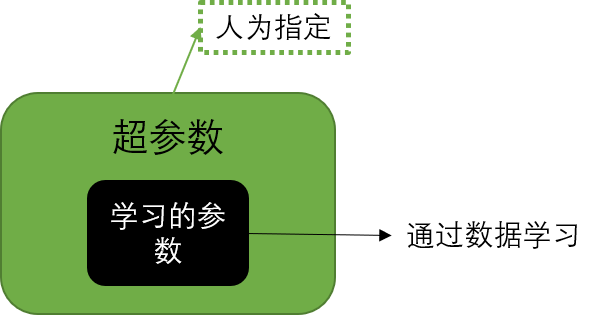
\includegraphics[width=.5\textwidth]{pics/model.png}
	\label{fig:model}
	\caption{模型的超参数与学习参数}
\end{figure}

一些值得注意的问题: 
\begin{itemize}
	\item LOOCV计算成本太高而且不同训练集之间的重合度太高
	\item K的选取. K太大, 投入的训练集也大, 得到的模型可能会有较小的偏差, 但是由于训练集之间的重叠度较高, 会存在较高的方差
\end{itemize}

\subsection{归一化 vs 标准化 定量的分析}
参考: \href{https://mp.weixin.qq.com/s/lO3Li7dWAvtzefVA_M0dJg}{https://mp.weixin.qq.com/s/lO3Li7dWAvtzefVA\_M0dJg}\\
\textbf{归一化: }将值变换到$[0, 1]$或者$[-1, 1]$之间, 使得不同类型的特征之间有了可比性, 对利用了样本之间距离的算法很重要. \textbf{标准化: }改变数据的统计特征, 如将均值和方差变为0和1. 在现实中, 一个变量极有可能是服从正态分布的. 


一些重要的结论: 
\begin{itemize}
	\item 对于不同的算法, 可能不同的缩放方法有不同的效果, 例如Tree-based模型对特征的尺度是不敏感的, 而一些依赖样本之间的距离的方法则对尺度很敏感, 如KNN、LR等; 
	
	\item 归一化容易受到异常值的影响, 可能会将数据点挤压到一起; 
\end{itemize}

二者的使用场景:
\begin{itemize}
	\item 标准化. 更好地保留了样本间的间距,因此在一些依赖距离度量的算法中,例如 分类, 聚类中最好使用规范化;
	
	\item 归一化. 如果数据不太符合正态分布, 或者对数据的范围有要求可以使用归一化;
\end{itemize}

\subsection{数据探索}
\paragraph{What?}数据探索是机器学习任务中的一个过程, 通过数据探索, 我们应该能够对数据有一个深入的认识. 很多人认为数据探索只是任务开始之前的一个步骤, 其实数据探索应该\textbf{贯穿整个任务的生命周期}. 在任务开始前, 对数据有个整体的把握, 知道数据的形式、数据量、数据的异常、缺失值、冗余等; 在完成任务的过程中, 发现当前使用的特征的特点, 特征的价值、关联等; 完成任务后, 分析特征的重要性、误差, 以及可能的优化方向. \textbf{数据探索, 是我们选用何种算法的依据, 以及算法模型中使用哪些特征. }

\paragraph{How?}
\subparagraph{数据初探}认识数据, 掌握原始数据的基本情况, 通过这一步, 我们要做到: 
\begin{itemize}
	\item 数据集的基本情况: 数据集有多大、数据的形式、数据的类型
	\item 重复值、缺失值、异常值: 去除重复值, 缺失值的处理, 缺失是否严重、是否有特殊含义, 发现异常值并处理
	\item 特征之间的冗余性: 是否有特征重复表达了
	\item 是否存在时间信息: 引入时间后, 处理会更复杂, 通常要进行相关性、趋势、周期和异常点的分析, 以及潜在的数据穿越问题
	\item 标签分布: 分类问题中类别分布是否均衡、回归问题中是否有异常值、值的分布情况、\textbf{是否需要进行目标转换}
	\item 训练集与测试集的分布: 训练集与测试集中标签的分布是否一致、两个数据集是否同分布
	\item 单变量/多变量分析: 特征的分布、特征之间的关系、特征与目标变量的关系
\end{itemize}
了解数据长什么样后, 我们才能知道\textbf{该选用哪个算法模型}、\textbf{该如何处理数据}、对数据进转换. 

\subparagraph{变量分析}分析特征的特点、特征之间的关联, 冗余性等. 主要可以分成: 
\begin{itemize}
	\item 单变量分析: 按照变量的取值, 可以将变量分为连续性和离散型. 连续性一般为数值, 离散型则比较多了, 如类别型、字符串、日期等. 单变量分析分析标签、特征的分布, 特征与目标的相关性等. 挖掘特征图用目标的关联, 可以帮助去除无效的特征, \textbf{找到有效的特征组合 (特征交叉) }, 如强相关加弱相关、强相关加强相关等
	
	\item 多变量分析: 分析特征变量之间的关系. 帮助我们发现哪些特征是冗余的, 进行特征组合, 发掘更高阶的特征
\end{itemize}

\subparagraph{模型分析}任务完成或者模型训练完后, 一般还需要对算法进行调整, 这时候就需要通过分析正在使用的模型有哪些缺点, 主要的方式有: 
\begin{itemize}
	\item 学习曲线: 发现是否存在过/欠拟合的问题
	\item 特征重要性分析: 通常在得到模型后, 我们可以获得特征的重要性, 分析特征的重要性是否符合实际情况、或者发现不符合直觉的深层现象、帮助我们选择特征
	\item 误差分析: 通过模型预测结果发现问题. 回归中看预测结果的分布, 分类中看混淆矩阵等. 借此来发现对于哪些样本表现不佳, 找到模型的弱点, 或者\textbf{为什么在这些样本上不佳的原因, 有时我们需要赋予这些 hard 样本更高的权重}
\end{itemize}





\subsection{Inductive Bias}
归纳偏置, 使用某个算法解决问题时所基于的假设, 类似于贝叶斯中的先验 (prior) , 与先验不同, 归纳偏置在学习过程中不会被更新, 而先验会不断被更新. 机器学习中常见的归纳偏置: 奥卡姆剃刀、CNN中的局部性、KNN中假设相似样本在特征空间中也是相邻的、SVM假设好的分类器应该是类别边界距离最大的等. 

\subsection{Covariate Shift}
协变量偏移, 指机器学习中训练集和测试集样本分布不一致的现象. 机器学习中通常假设训练和测试数据的分布是一致的, 在训练集学习的参数能否在测试数据上也有很好的表现呢?当训练集和测试集的分布不是那么相似时, covariate shift就出现了. 这里的数据分布不一致举个例子: 训练一个健康预测器, 训练集大多是 60 岁以下的, 但是测试集却大部分来自老年人. 

\subsubsection{怎么发现 Covariate Shift?}
做机器学习任务, 检验训练集和测试集的分布是很重要的, 其实一直不太了解如何验证两个数据集的分布是否一致. 验证是否发生了 Covariate Shift 其实也可以看作验证训练集和测试集的分布是否一致. 既然时验证分布是否一致, 那么就可以看成是一个分类任务, 训练一个分类器来判断一个样本是来自训练集和测试集. 具体做法: 从训练集和测试集中随机挑选等量的样本, 生成一个新的数据集, 给这个数据集中的每个样本增加一标签, 标识其来自训练集还是测试集, 之后就用这个新数据集进行训练, 训练完后计算模型的性能, 如果性能不错, 则说明出现了偏移. 

\subsubsection{怎么解决?}
怎么解决呢?
\begin{itemize}
	\item 训练集和测试集的分布不一致导致模型的参数泛化性能不佳, 可能是测试集中地某些样本在训练集中被“轻视”或“过度重视”了, 因此可以通过附加一个权重来解决该问题. 可参考: \href{https://blog.csdn.net/mao_xiao_feng/article/details/54317852}{covariate shift现象的解释}; 
	\item 丢弃那些导致偏移的且不重要的特征, 参考: \href{https://zhuanlan.zhihu.com/p/205183444}{Covariate Shift}. 
\end{itemize}

\subsection{机器学习中常用的算法指标及其应用场景}

% Please add the following required packages to your document preamble:
% \usepackage{multirow}
% \usepackage[table,xcdraw]{xcolor}
% If you use beamer only pass "xcolor=table" option, i.e. \documentclass[xcolor=table]{beamer}
\paragraph{Accuracy, Recall, Precision, F-score}

$ACC = \frac{TP + TN}{TP+FN+TN+FP}\quad R = \frac{TP}{TP+FN}\quad P = \frac{TP}{TP+FP}\quad F(\beta) = (1 + \beta^2)\frac{P \cdot R}{\beta^2 P + R}$. 混淆矩阵 (Confusion Matrix) 见表.\ref{tab:confusion_mat}. F-score是对R, P的一个综合评价, $\beta$度量了R 相对于 P的重要性, 可以理解为$\beta = \frac{importance(R) }{importance(P)}$, 则表示$\beta$越大, 我们越看重R. 

\begin{table}[h]
	\centering
	\caption{二分类混淆矩阵}
	\label{tab:confusion_mat}
	\begin{tabular}{|c|l|l|}
		\hline
		\multicolumn{1}{|l|}{}                          & \multicolumn{2}{c|}{Actual class (observation)}                                                                                   \\ \hline
		& tp (true positive) Correct result                          & fp (false positive) Unexpected result                                \\ \cline{2-3} 
		\multirow{-2}{*}{Predicted class (expectation)} & \cellcolor[HTML]{68CBD0}fn (false negative) Missing result & \cellcolor[HTML]{68CBD0}tn (true negative) Correct absence of result \\ \hline
	\end{tabular}
\end{table}

\paragraph*{关于$Precision$, $Recall$的选择?}这几个指标在很多任务中都有应用, , 但是不同的指标侧重于不同的方面, 比如P、R都有不同的侧重, 但看一个指标是比较片面的, 并不能反映出模型真实的效果. 有可能P很高, 但是R很低, 而在一些场景下R是很重要的. 

比如在金融风控等领域, 我们希望算法能够尽量识别出所有有可能有风险的用户, 这时候就侧重于 Recall, 即希望算法把所有的正样本 (通常有危险的, 需要被找出来的被标记为正样本) 都筛选出来, 即使将所有样本都标为正 (即 Recall=1) . 因为这种情况下, 可能漏掉一个正样本带来的代价是极大的, 通常筛选完之后还需要交给人工进行判断. 类似的场景还有癌症检测, 将一个没有癌症的判断为癌症没有很大关系, 但是将一个有癌症的判断为没有癌症则是很严重的, 会出人命的!!!

又比如在垃圾邮件分类中, 我们可能更侧重于Precision. 我们希望算法在识别垃圾邮件时不要把正常邮件错分了, 这个时候希望Precision尽可能高, 即使将所有样本标为负也没关系 (TP=0时可认为Precision=1) , 或者说算法只把自己十分确信为垃圾邮件的标为正, 尽量降低FP, 即尽量不要把正常邮件视为垃圾邮件, 不然错过了offer那可咋整!!!

通常, 将需要识别出的类别, 或者简单的说坏的一类为正样本, 为什么呢?因为好的漏掉一般不会产生啥大的影响, 但是坏的跑了课就不行了!当然, 也需要不同场景下选择合适的指标!!!

我们是贪心的, 因此就有了一些综合的指标, 比如F-score. 
Precision是以被分类的所有样本为分母, Recall则是以原本所有的positives元素为分母. 二者之间并没有建立直接联系, 如果一个分类器, Precision很高但是Recall很低, 或者Recall很高但是Precision很低, 这两种分类器都是不好的, 都是我们不希望的. 所以我们采用F1-Score来建立Precision和Recall的联系. 

\textbf{在数学中, 调和平均数是永远小于等于算术均值平均数的, 当用于求两个数的平均数时, 如果直接用算术平均作为结果, 那么两数之间的差异将被大的值削平, 而调和平均数则不会极大削平这种大的差异, 得到的结果更倾向于小的值}. 

\paragraph{Micro-F1 \& Macro-F1}基本的F1使针对二分类任务而言的, 在多分类中中, Micro-F1和Macro-F1是两种求多类别F1均值的方式. 
\begin{itemize}
	\item Micro-F1: 分别计算每个类别的$TP, FN, FP$, 再求整体的$Recall$, $Precision$, 再以整体的$P, R$来求$F1$, 得到Micro-F1. 在计算公式中考虑到了每个类别的数量, 所以适用于数据分布不平衡的情况; 但同时因为考虑到数据的数量, 所以在数据极度不平衡的情况下, \textbf{数量较多的类 (即常见的类) 会较大的影响到F1的值}
	\item Macro-F1: 分别计算每个类别的F1, 再求平均, 得到Macro-F1. 没有考虑到数据的数量, 所以会平等的看待每一类 (因为每一类的precision和recall都在0-1之间) , \textbf{会相对受高$Precision$和高$Recall$类 (即稀有的类) 的影响较大}
\end{itemize}
$Micro-F1$公式如下所示: 
$$
\begin{aligned}
	 Recall_{m i} &=\frac{\sum_i TP_{i}}{\sum_i TP_{i} + \sum_i FN_{i}} \\
	Precision_{m i} &=\frac{\sum_i TP_{i}}{\sum_i TP_{i} + \sum_i FP_{i}} \\
	Micro-F1 &= \frac{ Recall_{m i} \times Precision_{m i}}{Recall_{m i}+ Precision_{m i}}
\end{aligned}
$$
$Macro-F1$如下所示: 
$$
Macro-F1 &=2 \frac{ \sum_i F1_i}{N}
$$


\paragraph{ROC、AUC}接收者操作特征曲线 (recevier operating characteristic curve) , 用于反映一个而分类器的灵敏度 (sensitivity) 和特异度 (specificity) 之间的关系. 
$$
\begin{aligned}
	Sensitivity &= \frac{TP}{TP + FN}\\
	Specificity &= \frac{TN}{TN + FP}
\end{aligned}
$$
其中Sensitivity也就是TPR (True Positive Rate) , 也就是Recall, Specificity是TNR (True Negtive Rate) . ROC的横坐标是$1 - Specificity$, 即FPR (False Positive Rate, 即\textbf{负样本中有多少被分成了正样本}) , 纵坐标是Sensitivity. 横坐标表示的是负样本中被预测为正样本的比例, 纵坐标表示的是正样本中被预测为正样本的比例. 

ROC如Fig.\ref{fig:roc}所示. 

\begin{figure}[h]
	\centering
	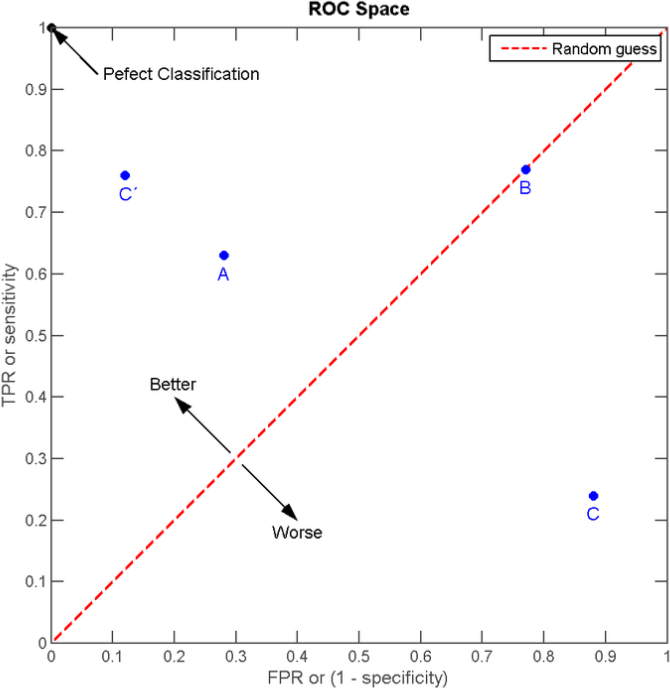
\includegraphics[width=.6\textwidth]{pics/roc.png}
	\caption{ROC}
	\label{fig:roc}
\end{figure}
ROC的绘制过程: 对于一个二分类问题, 使用一个分类器对样本集进行预测后, 可以得到每个样本属于正样本的概率, 此时我们还需要一个阈值来确定那些为正样本. 每选取一个阈值, 就可以得到一个 (TPR, FPR) 数值对. 当阈值从1到0不断减小时, 被确定为正样本的样本数不断增大, 其中TP和FP都会不断增大, 由于正负样本的数量是固定的 (即TPR, FPR的分母是固定的) , 则TPR和FPR都会不断增大. 那么, 
\begin{itemize}
	\item 当阈值为1时,  (几乎) 所有样本都为负样本, 则TPR约为0, 既然都为负样本那么FP也为0, 则FPR也为0
	\item 当阈值为0时, 所有样本都为正样本, 那么肯定所有的正样本都找出来了, 则TPR为1, 由于所有样本都预测为正样本, 那么肯定所有的负样本都预测为了正样本, 则FPR为1
\end{itemize}
因此, 在阈值从1到0的过程中,  (TPR, FPR) 不断增大, 从坐标 (0, 0) 到 (1, 1) , 如Fig.\ref{fig:threshold}所示, Fig.\ref{fig:threshold}上部分为负样本为正样本的概率的分布图 (即横坐标为正样本概率值, 纵坐标为对应的样本数量) , 下部分为正样本为正样本的概率的分布图, 可见, 当阈值为$B$时, 大部分正样本都被分为了正样本 (TP) , 小部分负样本被分为了正样本 (FP) . 由Fig.\ref{fig:roc-threshold}可见, 当阈值减小时,  (TPR, FPR) 的变化过程. 

\begin{figure}[h]
	\centering
	\subfigure[阈值变化与预测正负样本的分布]{
		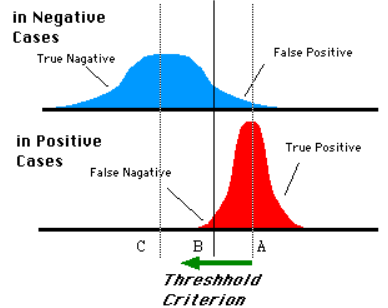
\includegraphics[width=7cm]{pics/threshold.png}
		\label{fig:threshold}
	}
	\quad
	\subfigure[阈值变化与ROC]{
		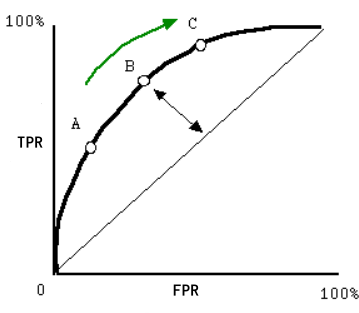
\includegraphics[width=7cm]{pics/roc-threshold.png}
		\label{fig:roc-threshold}
	}
	\caption{阈值变化}
	\label{fig:threshold-change}
\end{figure}
ROC是一个曲线, 那怎么作为一个指标呢? --- 取ROC与坐标轴围成的面积, 即\textbf{AUC (Area Under Curve) }. 由于ROC的绘制过程, 我们希望当阈值为接近0时, TPR尽量高, FPR尽量低 (其实不管阈值为何值, 都希望有这个效果) , 一个好的分类器的ROC的AUC应该尽量大. 

AUC的含义: 随机挑选一个正样本、一个负样本, 分类器分别给出一个分数, 正样本的分数大于负样本的分数的概率. \tbc{red}{强烈推荐}-相关证明: \href{http://vividfree.github.io/%E6%9C%BA%E5%99%A8%E5%AD%A6%E4%B9%A0/2015/11/20/understanding-ROC-and-AUC}{\tbc{red}{理解 ROC 和 AUC}} (以及 AUC 的简洁计算方式). 

\textbf{为什么要用ROC/AUC呢?}\newline
因为ROC曲线有个很好的特性: 当测试集中的正负样本的分布变化的时候, ROC曲线能够保持不变. 在实际的数据集中经常会出现类不平衡(class imbalance)现象, 即负样本比正样本多很多(或者相反), 而且测试数据中的正负样本的分布也可能随着时间变化. roc曲线不变原因: TPR和FPR是实际label内部的操作, 看混淆矩阵和tpr、fpr计算公式, 无论实际label比例怎么变化, tpr、fpr计算公式都是在实际为p或者n的内部计算的. AUC 关注的是样本间的排序效果. AUC 对正负样本比例的不敏感性: \href{https://blog.csdn.net/Leon_winter/article/details/104673047}{AUC: 直观理解AUC为何会对正负样本数分布不均匀情况鲁棒}. 

\textbf{如何使用ROC来选择模型?}\newline
当我们有多个分类器时, 给定一个数据集, 可以得到多条ROC曲线, 那么怎么来选择模型呢?一个很直观的想法是直接比较AUC. 但是在不同场景下, 我们要结合更看重的指标选择模型. 如Fig.\ref{fig:roc-cmp}所示, 当ROC不交叉时, 可以直接选择AUC高的, 当ROC交叉时则需要慎重考虑了. 当需要高的Sensitiviy时, 选择A, 需要高Specificity (即低FPR) 时选择B. 


\begin{figure}[h]
	\centering
	\subfigure[ROC不交叉]{
		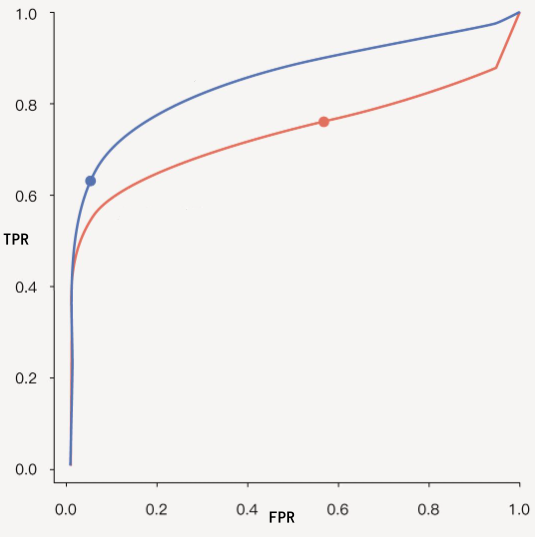
\includegraphics[width=7cm]{pics/roc1.png}
		\label{fig:roc1}
	}
	\quad
	\subfigure[ROC交叉]{
		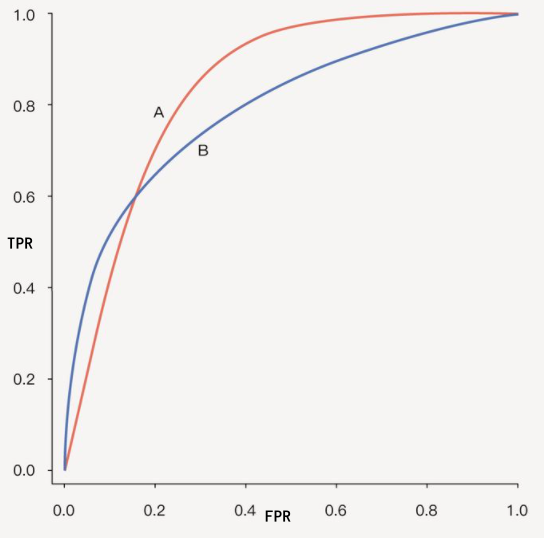
\includegraphics[width=7cm]{pics/roc2.png}
		\label{fig:roc2}
	}
	\caption{ROC比较}
	\label{fig:roc-cmp}
\end{figure}

参考资料: 
\begin{itemize}
	\item \href{https://blog.csdn.net/pipisorry/article/details/51788927}{分类模型评估之ROC-AUC曲线和PRC曲线}
	\item \href{https://zh.wikipedia.org/zh/ROC%E6%9B%B2%E7%BA%BF}{ROC曲线}
\end{itemize}


\paragraph{mIoU}
Mean Intersection over Union(MIoU, 均交并比), 为语义分割的标准度量. 其计算两个集合的交并比, 在\textbf{语义分割}的问题中, 这两个集合为真实值 (ground truth) 和预测值 (predicted segmentation) . 令$p_{ij}$表示实际类别为$i$, 预测类别为$j$的数量, 则
$$
mIoU = \frac{1}{C} \sum_{i=1}^{C} \frac{p_{ii}}{ \sum_{j=1}^{C} p_{ij} + \sum_{j=1} p_{ji} - p_{ii} }
$$
如下图Fig.\ref{fig:miou}所示: 
\begin{figure}[h]
	\centering
	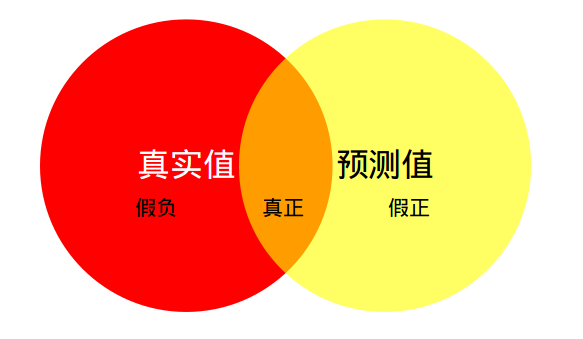
\includegraphics[width=.6\textwidth]{pics/miou.png}
	\caption{mIoU}
	\label{fig:miou}
\end{figure}
在\textbf{语义分割}中, 被分类的对象为每个像素, 真实标签为该像素所属的类别, 预测标签为预测的类别. 计算时, 可以先计算出混淆矩阵, 将对角线上的元素的值之和除以混淆矩阵中所有元素的和, 再除以类别数就是mIoU了. 注意, 在实际计算中, 要注意除零的情况. 

\paragraph{Dice}
有Dice系数和Dice loss之分. 
Dice系数是一种集合相似度度量函数, 通常用于计算两个样本的相似度, 取值范围在[0,1], 计算公式如下: 
$$
dice(x, y) = \frac{2|x \cap y|}{|x| + |y|}
$$
在\textbf{语义分割}中, $x, y$可以分别代表预测的分割结果、真实的分割, 分别以矩阵的形式表示. 那么, 计算模型的分割效果可以为: 
$$
dice(pred, ground) = \frac{2(pred \cdot ground).sum()}{pred.sum() + ground.sum()}
$$
其中, $\cdot$和\textit{.sum()}分别表示矩阵的逐元素乘积、逐元素求和. 
Dice loss则是: $1 - dice(pred, ground)$, Dice loss 首次在VNet中提出. 

在图像分割实践中, 可以用Dice loss或者交叉熵损失函数作为目标函数, 但是由于交叉损失函数的梯度形式更优, 更倾向于选择交叉熵损失函数. 
Dice Loss特点: 
\begin{itemize}
	\item 训练误差曲线非常混乱, 很难看出关于收敛的信息. 尽管可以检查在验证集上的误差来避开此问题
	\item Dice Loss比较\textbf{适用于样本极度不均的情况}, 一般的情况下, 使用 Dice Loss 会对反向传播造成不利的影响, 容易使训练变得不稳定
	\item Dice对mask的内部填充比较敏感
	
\end{itemize}
作为Dice loss的一个替代, 可以使用cross entropy loss. 原因: 
\begin{center}
	使用交叉熵做损失函数时, 在反向传播时, 计算得到的梯度的形式是类似于 (p-t) 的, 其中$p, t$分别是预测值和标签. 而dice loss, 如果将其写成$\frac{2pt}{p^2+t^2}$ 或 $\frac{2pt}{p+t}$的形式, 则在反向传播时, 梯度大概时这个样子的:  $\frac{2t(t^2-p^2)}{(p^2+t^2)^2}$ 或 $\frac{2t^2}{(p+t)^2}$. 这样的梯度有什么问题呢?当$p, t$都很小时, 梯度可能会变得很大, 这也是\textbf{dice loss在训练过程中不稳定的原因}了. 
\end{center}



\paragraph{Rand Error}
Rand Error是以Rand Index (兰德系数) 为基础的. Rand Index用于衡量两个数据簇之间的相似性. Rand Index的定义: 
对数据点集进行分类时, 用a表示实际为同一类, 预测时也为同一类的数据点对 (pair) 的数量, b表示实际为不同类, 预测时也为不同类的数据点pair的数量, 则
%\binom{n}{k}\qquad\mathrm{C}_n^k
$$
RI(Rand Index) = \frac{a + b}{\mathrm{C}_n^k}
$$
Rand Error定义为: 
$$
RE = 1 - RI
$$
RE可以用于衡量图像分割算法的效果. 可以参考: \href{http://www.otlet-institute.org/wikics/Clustering_Problems.html#toc-Subsection-4.1}{Rand Index计算}. 

\paragraph{Hausdorff 距离} 可以用于衡量两个点集之间的距离, 定义如下, 其中$\boldsymbol{X}, \boldsymbol{Y}, d(x, y)$表示两个点集和点之间的距离度量函数: 
$$
d_{H}(X, Y) = \max (d_{X Y}, d_{Y x}) = \max \left\{\underset{x \in X}{\max } \min _{y \in Y}d(x, y),\quad \max _{y \in Y} \min _{x \in X} d(x, y)\right\}
$$
\textbf{Dice缺陷在于对边界的刻画不敏感}, 注意力主要集中在mask的内部. 而Hausdorff距离作为形状相似性的一种度量, 能够为Dice做出较好的补充. 
\begin{figure}[h]
	\centering
	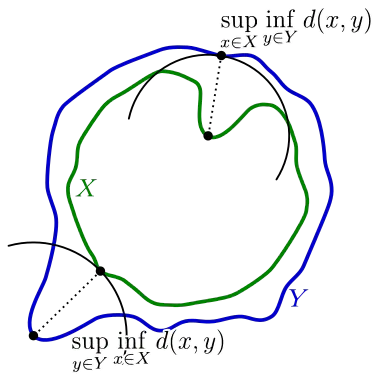
\includegraphics[width=.5\textwidth]{pics/Hausdorff distance.png}
	\caption{Hausdorff Distance}
	\label{fig: hausdorff distance}
\end{figure}

\paragraph{MRR}
Mean Reciprocal Rank, 常用来衡量搜索算法效果的指标, 目前被广泛用在允许返回多个结果的问题, 或者目前还比较难以解决的问题中 (由于如果只返回top 1的结果, 准确率或召回率会很差, 所以在技术不成熟的情况下, 先返回多个结果) . 在这类问题中, 系统会对每一个返回的结果给一个置信度 (打分) , 然后根据置信度排序, 将得分高的结果排在前面返回. 核心思想很简单: 返回的结果集的优劣, 跟第一个正确答案的位置有关, 第一个正确答案越靠前, 结果越好. 定义如下: 
$$
MRR = \frac{1}{|Q|} \sum_{i=1}^{|Q|} \frac{1}{rank_i}
$$
其中$Q$为查询集合, $rank_i$是第$i$个查询的结果集中正确结果的排名. 

\paragraph{AP}
Average Precision, 平均精确率. 对于二分类问题, 给定样本真实标签$\{y_1, ..., y_n\}$和模型预测的正样本置信度$\{c_1, ..., c_n\}$, 计算AP: 
\begin{enumerate}
	\item 按照置信度从大到小对样本进行排序, 令排序后的样本的置信度为$\{c_1, ..., c_n\}$
	\item 令 $i=1$, 重复执行: 
	\begin{enumerate}
		\item 以$c_i$为阈值, 得到预测的正负样本, 即前$i$行预测为正样本, 之后的均为负样本
		\item 计算当前阈值下的Recall和Precision
		\item $i += 1$
		\item 当$i > n$则结束循环
	\end{enumerate}
	\item 排序后的每个样本都对应一个(Recall, Precision)对, 即$\{(r_1, p_1), ..., (r_n, p_n)\}$
	\item 上一步得到的Recall列表$\{r_1, ..., r_n\}$中的元素$r_i$与$r_{i-1}$做差, 设$r_0 = 0$, 则可以得到$\{d_1, ..., d_n\}$, 其中$d_i = r_i - r_{i-1}$
	\item 求和: $AP = \sum_{i=1}^n d_i \cdot p_i$
\end{enumerate}
如Fig.\ref{fig:ap}所示, 该表是按照置信度排序后的样本, correct列表示该样本的真实标签, P、R列是按照上述方式计算出来的Recall和Precision. 
\begin{figure}[h]
	\centering
	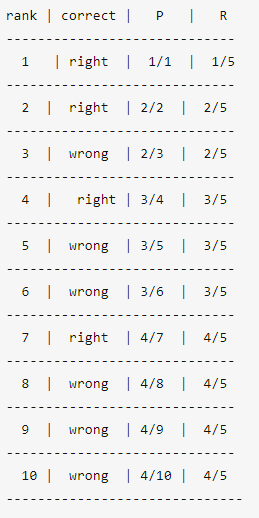
\includegraphics[width=.3\textwidth]{pics/AP.png}
	\caption{AP计算示例}
	\label{fig:ap}
\end{figure}

\paragraph{MAP}
Mean Average Precision, 是AP的均值. AP通常是针对单个类别而言的, 当有多个类别时, 分别计算每个类别的AP, 再进行算术平均. 

\tbc{red}{注意: }AP和MAP常用在目标检测和信息检索领域中. 
\begin{itemize}
	\item 目标检测领域中, 对于一个类别, 可能会检测出多个检测框, 每个检测框可以根据IoU来判断检测框的真实标签是1还是0 (针对一个类别的检测而言, \tbc{green}{因为目标检测中的Ground Truth也是一个边界框, 所以不需要和边界框完全一致才作为正样本, 只要IoU大于一定阈值即可}) , 每个检测框还对应一个置信度. 此时即可按照上述方式计算该类别的AP
	\item 在信息检索领域, 对于一个查询$q$, 通常希望模型能够给出top K个结果 (\tbc{red}{有序的}) . 若$q$真实的有序搜索结果列表为$\{d_1, ..., d_m\}$, 则可以对这K个结果的标签, 由于模型的输出已经是排好序的, 故可以直接计算AP. 对于多个查询, 则计算每个查询的AP后再取平均
\end{itemize}
总而言之, 根据某种方法判定样本的真实标签 (如目标检测中通过IoU判定、分类任务中给定的标签、搜索中给定的真实搜索列表等) , 再根据置信度进行排序 (如目标检测中的置信度、分类任务中输出的分数、搜索中直接给出的排序等) , 计算每个位置处的$(recall, precision)$, 按照上述方式即可算出AP. 


\paragraph{DCG、NDCG}
Discounted Cumulative Gain, 折扣累计增益. 在介绍DCG之前有必要先介绍一下CG, Cumulative Gain, 即累计增益. 这两个指标主要用于搜索领域. 对于模型返回的$p$个结果 (\tbc{red}{有序的}) , 每个位置处的结果与查询的相关性为$rel_i$, 则该结果的CG为: 
$$
CG_p = \sum_{i=1}^p rel_i
$$
很明显, CG没有考虑结果的先后顺序, 在搜索中, 结果的顺序是至关重要的, 因此产生了DCG: 同一个相关度, 排名越后则增益越小, 即与所处排名成反比. 
$$
DCG = \sum_{i=1}^p \frac{rel_i}{\log_2(i+1)}\qquad or\qquad \sum_{i+1}^p \frac{2^{rel_i} - 1}{\log_2(i+1)}
$$
通常, 不同的查询对应的结果列表是不一样长的 (\tbc{green}{不同长度的搜索结果对应的DCG值范围不一样, 无法直接比较, 例如长的结果列表DCG最大可为10, 短的最大可为5, 前者的DCG为4和后者的DCG为4并不代表二者的结果列表质量一样}) , 因此不能将DCG用于评价结果列表长度不同的查询效果, 因此需要对DCG进行归一化, 即NDCG (Normalized DCG, 归一化折扣累计增益) , 
$$
NDCG = \frac{DCG}{IDCG}
$$
其中IDCG为理想情况下的折扣累计增益, 表示真实的结果列表的DCG, 计算方式为取真实结果列表的前$p$个结果计算DCG, 即
$$
IDCG = \sum_{i=1}^p \frac{2^{rel_i} - 1}{\log_2(i+1)}
$$

\tbc{red}{注意: }MAP和NDCG都可以用于衡量搜索结果的质量, 但是MAP只支持两种相关性: \{相关, 不相关\}, NDCG可以支持多种相关性得分, 如1-5. 


\paragraph{GAUC}Group AUC, 是 AUC 的一个变体, 在推荐系统领域中更准确地衡量模型得性能. 以 CTR 估计任务为例, 数据集中包含了不同用户得正负样本, 模型给出每个样本属于正样本得一个概率值后计课计算一个 AUC. 但是很明显, AUC 将不同用户的正负样本混合起来了, 即期望任一个用户的正样本的概率大于任一个用户的负样本的概率, 但推荐中更关注的是对于一个用户, 模型对其正负样本的排序能力. 其定义为: 
$$
GAUC = \frac{\sum_{u_i} w_{u_i} \cdot AUC_{u_i}}{\sum_{u_i} w_{u_i}}
$$
其中 $w_{u_i}}$ 是 $u_i$ 的权重, 这个值可以是用户的样本的数量. 可以看出, GAUC 是定义在 AUC 上的, 即计算模型对每个用户的样本的排序能力. 其实可用通过这个指标发现模型对哪一类用户有较好的性能, 那是不是可以以此为基础进行多个模型的融合呢?

\subsection{常用数据增强手段}
增强之前, 先想一想: 真的需要增强数据吗 (通常来说是的) ?需要增加的多少数据?需要增加什么样的数据 (并不是什么样的数据都可以, 主要考虑应用场景中一般会出现的数据即可) ?
\paragraph{仿射变换}
仿射变换 (Affine Transformation) 是指在二维向量空间中进行一次线性变换(乘以一个矩阵)和一次平移(加上一个向量), 变换到另一个向量空间的过程. 
$$
\left[\begin{array}{l}
	u \\
	v \\
	1
\end{array}\right]=\left[\begin{array}{ccc}
	a_{1} & b_{1} & c_{1} \\
	a_{2} & b_{2} & c_{2} \\
	0 & 0 & 1
\end{array}\right]\left[\begin{array}{l}
	x \\
	y \\
	1
\end{array}\right]
$$

图解, 放射变换的种类也如Fig.\ref{fig:affine}所示: 
\begin{figure}[h]
	\centering
	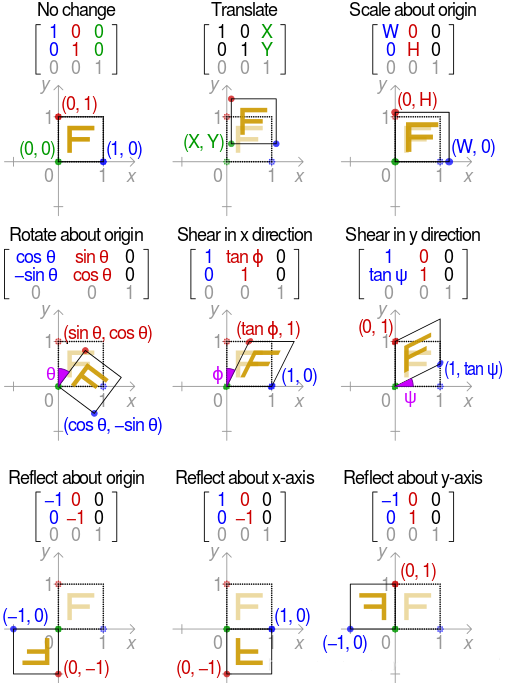
\includegraphics[width=.8\textwidth]{pics/affine.png}
	\label{fig:affine}
	\caption{仿射变换}
\end{figure}

\paragraph{弹性形变\cite{simard2003best}}
最早是从UNet中了解到弹性形变, 在细胞分割中, 弹性形变发挥了重要作用; 弹性形变也用在手写数字识别中. 可以发现, 在这两种任务中, 任务所涉及的对象并不是刚体, 简单的仿射变换并不能满足我们的需求. 弹性形变所针对的数据特点: 对象不是刚体, 可能在不同的场景下会有形变. 

弹性形变流程: 
\begin{itemize}
	\item 对图像imageA进行仿射变换, 得到imageB
	\item 对imageB图像中的每个像素点随机生成一个在x和y方向的位移, $\Delta \mathrm{x}$和$\Delta \mathrm{y}$. 其位移范围在(-1, 1)之间, 得到一个随机位移场(random displacement fields)
	\item 用服从高斯分布的$N(0, \delta)$对step2中生成的随机位移场进行卷积操作(和CNN中的卷积操作一样, 说白了就是滤波操作). 我们知道δ越大, 产生的图像越平滑. 下图是论文中的不同δ值对随机位移场的影响, 下图左上角为原图, 右上角为$\delta$较小的情况(可以发现, 位移方向非常随机), 左下角和右下角为较大的不同$\delta$值
	\item 用一个控制因子$\alpha$与随机位移场相乘, 用以控制其变形强度
	\item 将随机位移场施加到原图上, 具体是\textbf{怎么施加的呢}?首先, 生成一个和imageB大小一样的meshgrid网格meshB, 网格中的每个值就是像素的坐标, 比如说meshgrid网格大小为512x512, 则meshgrid中的值为(0, 0), (0, 1), ..., (511, 0), (511, 511), 然后将随机位移场和meshB网格相加, 这就模拟了imageB中的每个像素点在经过随机位移场的作用后, 被偏移的位置, meshB与随机位移场相加后的结果记做imageC
	\item 弹性变形最终输出的imageC中每个位置的灰度值大小, 组成一副变形图像, 现在imageC中每个像素点存储的是$(\mathrm{x}+\Delta \mathrm{x}, \mathrm{y}+\Delta \mathrm{y})$, 如下图中的$\mathrm{A}^{\prime}$, 那怎么转化成灰度值呢, 依据论文, 作者是根据imageB中的B位置的双线性插值灰度值作为$\mathrm{A}^{\prime}$点的像素灰度值大小 (如Fig.\ref{fig:elastic-deform}所示) , 最终将imageC输出得到变形图像
\end{itemize}
\begin{figure}[h]
	\centering
	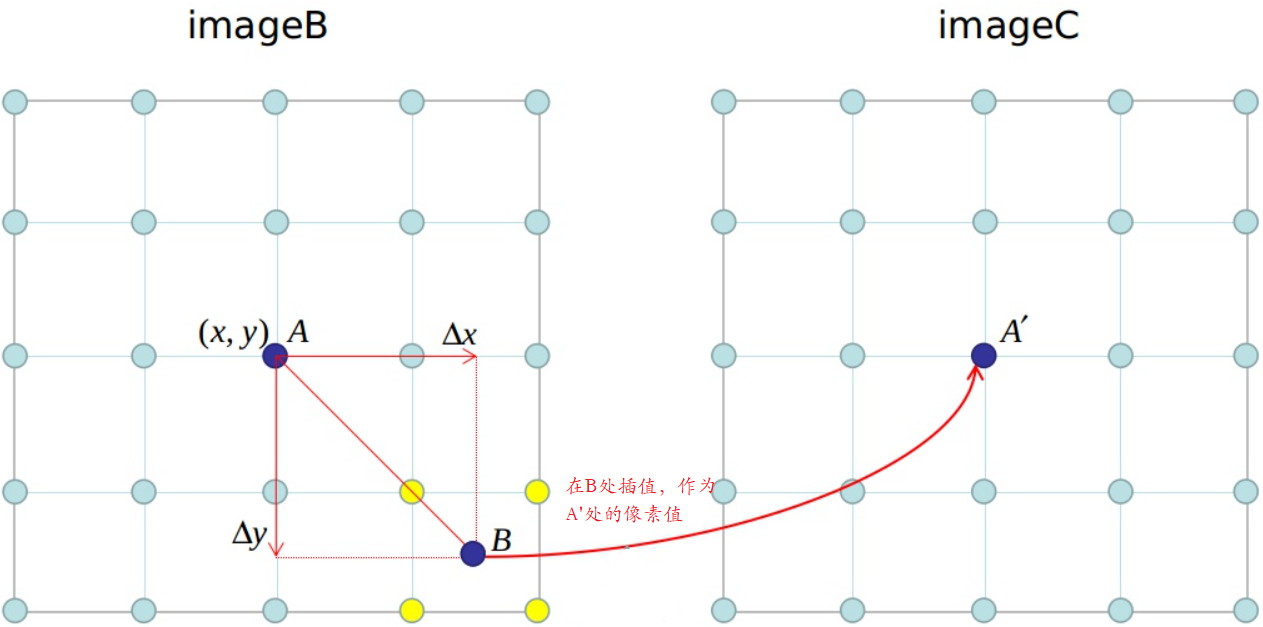
\includegraphics[width=.8\textwidth]{pics/elastic_deform.png}
	\label{fig:elastic-deform}
	\caption{弹性形变}
\end{figure}
参考: \href{https://zhuanlan.zhihu.com/p/342274228}{数据增强: 弹性变形(Elastic Distortion)}. 

\paragraph{增加噪声}
如椒盐噪声. 

\paragraph{GAN}


\subsection{类别不平衡问题}
指的是监督学习中, 不同类别的样本数目具有较大的差异 (样数据分布与均匀分布差异较大) . 
\paragraph{类别不均衡可能造成的问题}
\begin{itemize}
	\item 一些评价指标可能失效. 例如在癌症检测中, 可能$99\%$的样本都是0, 只有$1\%$的样本为1, 这个时候即使将所有样本预测为0也能有很好的acc, 但是漏检是很严重的!类别不平衡使得一些评价指标并不能反映模型真是的能力
	\item 
\end{itemize}

\paragraph{决解办法}
\subparagraph{数据角度}
中心思想就是直接改变数据分布. 
\begin{itemize}
	\item 获取更多数据, 使数据分布趋向于均衡
	\item 上采样. 通过一些方法, 使得占少数的类别 (minority类) 的样本数增加, 常用的方法: 
	\begin{itemize}
		\item 重复采样minority类, 使其样本数增加
		\item 合成的方法. 根据已有数据集生成新的样本, 如SMOTE方法及其变体
		\item 基于聚类. 分别对major和minority类进行聚类, 再通过过采样的方法使得major和majority中各个簇的数量相等, 例如原本major类聚类后样本数目比为1:2:3, minority类聚类后为1:2, 通过过采样的方法, 先使majority与minority样本数相等, 再使类内部各个簇的数目相等. 这样不仅可以解决类别间的不平衡, 还可以解决类内部的不平衡
	\end{itemize}
	\item 下采样. 通过一些方法把占多数的类别 (major类) 的样本数降低. 下采样的方法有很多
	\begin{itemize}
		\item 随机下采样, 从major类中随机保留一部分样本
		\item 基于临近样本, 来选择保留哪些major类样本
		\item 基于聚类, 对major类进行聚类, 使其具有N (minority类样本数) 个簇, 用这N个簇的中心作为major类采样后的样本
	\end{itemize}
\end{itemize}

\subparagraph{算法角度}
\begin{itemize}
	\item 选择对数据倾斜相对不敏感的算法, 如树模型等
	\item 在下采样时会损失一部分信息, 可以从major类中采样多个数据集来学习不同的模型, 即集成学习 (Ensemble集成算法) . 首先从多数类中独立随机抽取出若干子集, 将每个子集与少数类数据联合起来训练生成多个基分类器, 再加权组成新的分类器, 如加法模型、Adaboost、随机森林等
	\item 将任务转换成异常检测问题. 譬如有这样一个项目, 需要从高压线的航拍图片中, 将松动的螺丝/零件判断为待检测站点, 即负样本, 其他作为正样本, 这样来看, 数据倾斜是非常严重的, 而且在图像质量一般的情况下小物体检测的难度较大, 所以不如将其转换为无监督的异常检测算法, 不用过多的去考虑将数据转换为平衡问题来解决
\end{itemize}

\subparagraph{评价指标角度}
\begin{itemize}
	\item 混淆矩阵
	\item F-score
\end{itemize}

\subsection{特征选择的方法}
机器学习中, 面对成千上万的特征, 选择哪些进行保留是一个需要我们主动去抉择的问题. 既然是选择, 那肯定是要有一个明确的评判标准的. 

\subsubsection{过滤法}


\subsubsection{包装法}

\subsubsection{嵌入法}

\subsection{常用聚类算法}

\subsubsection{基于层次的聚类}
试图在不同层次上进行聚类, 从而形成树形的聚类结构. 数据集的划分可以自底向上也可以自底向下. 常见的有: Agglomerative 、Divisive、BIRCH、ROCK、Chameleon. 

\paragraph{优点}可解释性好 (如当需要创建一种分类法时) ; 还有些研究表明这些算法能产生高质量的聚类, 也会应用在上面说的先取 K 比较大的 K-means 后的合并阶段; 还有对于 K-means 不能解决的非球形族就可以解决了.  

\paragraph{缺点}时间复杂度比较高. 

\subsubsection{基于划分的聚类}
首先要确定簇的数量, 然后初始化簇的中心点, 再然后依据预先定好算法对数据点进行迭代重置 (即重置其所属的簇) , 直到最后到达“类内的点都足够近, 类间的点都足够远”的目标效果. 常见的有: K-means、K-means++、K-medoidsk-modes、k-medians、kernel k-means. 

\paragraph{特点}能够发现数据集中的球状簇, 因为通常是根据样本与中心的距离来划分的, 因此簇的表面通常是球面. 

\paragraph{优点}算法简单, 效率还可以. 

\paragraph{缺点}数据集较大时可能容易陷入局部最优 (\textcolor{red}{\textbf{为啥}}) ; 需要预先设定簇的数量 (看这些算法以 $k$ 打头就知道啦) ; 对异常值较敏感; 只适用于可计算相似性的样本空间. 
	
\subsubsection{基于密度的聚类}
定一个距离半径, 最少有多少个点, 然后把可以到达的点都连起来, 判断为同类. 常见的有: DBSCAN、OPTICS、DENCLUE. 

\paragraph{特点}能够对流形的数据进行聚类. 
	
\paragraph{优点}能够发现任意形状的簇, 对噪声不敏感. 

\paragraph{缺点}聚类的结果与参数有很大的关系; 当聚类的稀疏程度不同时, 相同的判定标准可能会破坏聚类的自然结构, 即较稀的聚类会被划分为多个类或密度较大且离得较近的类会被合并成一个聚类. 
	
\subsubsection{基于网格的聚类}
数据空间划分为网格单元, 将数据对象集映射到网格单元中, 并计算每个单元的密度. 根据预设的阈值判断每个网格单元是否为高密度单元, 密度足够大的网格单元形成簇. 常见的有: STING、WaveCluster、CLIQUE. 

\paragraph{优点}速度很快. 

\paragraph{缺点}参数敏感、无法处理不规则分布的数据、维数灾难等; 这种算法效率的提高是以聚类结果的精确性为代价的. 经常与基于密度的算法结合使用. 
	
\subsubsection{基于模型的聚类}
为每簇假定了一个模型, 寻找数据对给定模型的最佳拟合, 这一类方法主要是指基于概率模型的方法和基于神经网络模型的方法, 尤其以基于概率模型的方法居多. 这里的概率模型主要指概率生成模型 (generative Model) , 同一 "类" 的数据属于同一种概率分布, 即假设数据是根据潜在的概率分布生成的. 常见的有: GMM) 、SOM (Self Organized Maps) . 

\paragraph{优点}对”类“的划分不那么”坚硬“, 而是以概率形式表现, 每一类的特征也可以用参数来表达. 

\paragraph{缺点}执行效率不高, 特别是分布数量很多并且数据量很少的时候. 

主要参考: \href{https://blog.csdn.net/weixin_45440065/article/details/106358007}{聚类总结: 分类、优缺点、适用场景总结}、\href{https://blog.csdn.net/count_on_me/article/details/82193745}{聚类及聚类算法的分类}. 

\subsection{类别变量的编码方法}
\subsubsection{one-hot}
这个就很简单了, 将一个类别变量展开成一个向量, 向量的长度等于类别变量的基数. 经过独热编码后, 一个类别变量变成了一个向量, 很明显这增加了数据的维度, 而且编码后的数据是很稀疏的. 

\subsubsection{目标编码}
Target Encoder 是一种有监督的编码方式, 适用于分类和回归问题, 主要针对定类变量. 考虑分类问题. 假设在分类问题中, 目标 $y$  一共有 $C$ 个类别, 具体的一个类别用 $c$ 表示, 为了简化讨论, 当前考虑一个 $c$. 同时假设某一个定性特征 $f$ 中一共有 $K$ 个不同的类别, 具体的一个类别用 $k$ 表示. 针对一个目标 $c$, 目标编码将 $f$ 转化为一个后验概率 $P(y = c | f=k)$. 因此, 一个 $C$ 个类别的任务, 可以将 $f$ 转化成 $C-1$ 个特征, 每个特征针对一个目标进行编码. 即 $P(y=c_i | f=k), i=1, ..., C-1$. 

但是这样的做法有一个问题, 经过目标编码后的特征与目标有很强的相关性, 容易发生过拟合. 可以对目标编码进行平滑: 
$$
P = (1-\lambda) \cdot P(y = c) + \lambda \cdot P(y=c | f=k)
$$
一个特征类别在训练集内出现的次数越多, 其后验概率的可信度越高, 所以其权重也应该适当增大, 即此时 $\lambda$ 应该越大; 相反, 如果当一个特征类别在训练集内出现的次数较少的时候, 其后验概率的可信度较低, 所以我们应该让正则项更强一些, 即应该减小 $\lambda$. 那 $\lambda$ 应该如何取值呢?$\lambda$ 应该是一个关于某个特征类别在训练集中出现的次数 $n$ 的函数, 输出是对于这个特征类别的先验概率的权重的函数. 一种常用的计算方式: 
$$
\lambda (n) = \frac{1}{1+e^{-\frac{n-\beta}{\alpha}}}
$$
其中引入了两个参数 $\alpha, \beta$. 很明显, 当 $n > \beta$ 时 $\lambda > 0.5$, 即后验概率占比更大, 反之亦然. $\alpha$ 用于控制拐点处的斜率, 越小, 斜率越大.  

\subsubsection{贝叶斯目标编码}

\subsubsection{留一编码}

\subsubsection{证据权重}

\subsubsection{非线性 PCA}

\subsubsection{Embedding}

\subsection{为什么分类问题使用交叉熵而不使用 MSE?}
MSE 作为损失函数是非凸的, 不容易求解, 容易得到局部最优解; 而交叉熵损失函数是凸函数. 

MSE 求导后, 梯度与 sigmoid 的导数有关, 容易落在 sigmoid 的平坦区, 导致梯度很小, 引发梯度消失问题; 交叉熵求导后梯度为残差, 误差越大更新越快, 误差越小更新越慢. 

交叉熵衡量的是预测的分布与真实分布的距离, 更符合分类问题的预测目标.

\subsection{为什么要将连续特征离散化后输入到线性模型中?}
连续值经常离散化或者分离成 “箱子” 进行分析, 为什么要做数据分桶呢?
\begin{itemize}
	\item 离散后稀疏向量内积乘法运算速度更快, 计算结果也方便存储, 容易扩展; 
	
	\item 离散后的特征对异常值更具鲁棒性, 如 age>30 为 1 否则为 0, 对于年龄为 200 的也不会对模型造成很大的干扰; 
	
	\item LR 属于广义线性模型, 表达能力有限, 经过离散化后, 每个变量有单独的权重, 这相当于引入了非线性, 能够提升模型的表达能力, 加大拟合; 
	
	\item 离散后特征可以进行特征交叉, 提升表达能力, 由 M+N 个变量编程 M*N 个变量, 进一步引入非线形, 提升了表达能力; 
	
	\item 特征离散后模型更稳定, 如用户年龄区间, 不会因为用户年龄长了一岁就变化; 
	
	\item 特征离散化以后, 起到了简化了逻辑回归模型的作用, 降低了模型过拟合的风险; 
\end{itemize}


\subsection{分类模型与排序模型的异同分析}
\textbf{注意}: 这一节内容主要参考\href{https://zhuanlan.zhihu.com/p/502638808?utm_source=wechat_session&utm_medium=social&utm_oi=797192809567354880&utm_campaign=shareopn}{这里}.

在初入推荐系统这个坑时就思考过推荐和搜索的差异与异同, 那时我肯定想不到现在就在做搜索相关的实习. 缘分呐, 搜索!

不管在推荐还是搜索中, 都可以归结为 \textit{Learning To Rank}(LTR). LTR 通常由三种形式: Point-Wise, Pair-Wise 和 List-Wise. 推荐中, 排序的依据通常是 Point-Wise 形式的, 很多情况下就是 CTR, 这个问题可以看作是一个二分类的问题. 在搜索中, 就我目前了解到的情况来看, 更多的是 Pair-Wise 的 (仅就我目前了解到的情况).

\subsubsection{建模角度}
就二分类而言, 大多数模型最后输出的概率值都是通过 \textit{sigmoid} 得到的, 这就隐含了一个假设, 即假设样本为正样本的概率服从二项分布. 以逻辑回归为例, 在进入 \textit{sigmoid} 之前, 模型的值表示的是对数几率, 即 LR 线性部分预测的是对数几率. 真实的 CTR 模型也是类似的含义.

排序模型, 可以采用 LTR 的三种形式, 但使用较多的是 Pair-Wise, 这里就以这个为例吧. 在 Pair-Wise 中, 对于两个文档, 预测的是偏序关系是否成立:
$$
P_{i j} = P_{i} > P_{j}
$$
$P_{ij}$ 表示的是 $i$ 比 $j$ 排名更前的概率. 其实 $P_{ij}$ 也可以看作是一个分类变量, 但此时我们的样本是 $(i, j, P_{ij})$. 因此, 类比于二分类中的交叉熵损失:
$$
PairLoss = \sum_{(i, j) \in \{pairs\}} -P^\prime_{ij} \log P_{ij} - (1 - P^\prime_{ij}) \log (1 - P_{ij})
$$

综合对比来看, 推荐中的 Point-Wise 和搜索中的 Pair-Wise, 都可以看作是一个二分类变量, 差别在于二者的样本上. 推荐中估计的是单个样本的点击率, 搜索中估计的样本对的偏序关系是否成立. \textbf{\textcolor{red}{这二者来排序有啥不同呢?}} 在分类模型中, 要对两个样本都有准确的预估才能保持正确的派内需关系, 其要求更高; 而 Pair-Wise 可以看作分类模型的一个简化版本, 只要求偏序关系正确, 不要求对单个样本的预估绝对准确.

\subsubsection{事件之间的相互独立性假设} 
其实从二者的建模角度来看就可以看出, 分类模型假设各个样本之间是相互独立的 --- 独立同分布; Pair-Wise 则建立在同组 (同一个 query) 样本可以比较的基础上. 

\subsubsection{参数更新方式}
假设 $f$ 是要学习的模型, 在分类中代表分类模型, Pair-Wise 中代表对每个文档进行打分的模型 (类似于双塔). 则损失函数对参数的导数为:
$$
\frac{\partial L}{\partial w}=\frac{\partial L}{\partial f} \frac{\partial f}{\partial w}
$$

则 Point-Wise 的参数更新为:
$$
\mathrm{w}_{\mathrm{i}}^{\mathrm{t}+1}=w_{i}^{t}+\eta \frac{\partial L}{\partial f} \frac{\partial \mathrm{f}}{\partial w_{i}^{t}} \mathrm{x}_{\mathrm{i}}
$$

Pair-Wise 的参数更新为:
$$
\mathrm{w}_{\mathrm{i}}^{\mathrm{t}+1}=w_{i}^{t}+\eta \frac{\partial L}{\partial\left(f^{+}-f^{-}\right)} \frac{\partial\left(f^{+}-f^{-}\right)}{\partial w_{i}^{t}}\left(\mathrm{x}_{\mathrm{i}}^{+}-\mathrm{x}_{\mathrm{i}}^{-}\right)
$$
其中 $f^+, f^-$ 分别表示排名在前, 在后的样本的打分. 可见, 二者的偏序关系越显著, 参数更新的幅度越大.

\subsection{WOE, IV}
WOE, Weight of Evidence, 常用在风险评估、授信评分卡等领域. 

WOE是对原始自变量的\textbf{一种编码形式}, 要对一个变量进行 WOE 编码, 需要首先把这个变量进行离散化. 以二分类为例, 当拿到了一个离散变量, 对其进行 WOE 编码地过程: 按照变量的取值对数据集进行划分, 统计每个取值里正负样本的数量及在总的正负样本里的占比. 比如说, 变量 A 的取值 $a_1$ 中, 正负样本量分别是 $p, n$, 在总的正负样本量分别为 $P, N$, 则 A 变量的 $a_i$ 的 WOE 编码为 $ln \frac{p / P}{n / N}$. 通过 WOE 的计算公式也可以看出, 通常会在计算时加入平滑项避免 $p, n$ 为 0  的情况.

WOE 编码的好处:
\begin{itemize}
	\item WOE 是一种比较好的把自变量转化为与\textbf{对数几率}线性相关的有效形式;
	
	\item 所有自变量被 WOE 编码标准化后, 求解得到的系数值取值都在同一范围, 可以直接比较不同自变量对 odds 的影响;
	
	\item WOE 能反映自变量的贡献情况. 自变量内部 WOE 值的变异 (波动) 情况, 结合模型拟合出的系数, 构造出各个自变量的贡献率及相对重要性. 一般地, 系数越大, WOE 的方差越大, 则自变量的贡献率越大;
\end{itemize}

IV, Information value, 可通过 WOE 加权求和得到, 衡量自变量对因变量的预测能力, 可用于筛选变量. IV 是在 WOE 的基础上计算得到的. 还是刚刚的例子, 变量 A 的取值 $a_i$ 的 IV 计算为: $(\frac{p}{P} - \frac{n}{N}) \cdot WOE_{a_i}$. 

那么如何通过 IV 进行变量筛选呢? 对于一个 $n$ 个取值的离散变量, 其 IV 值计算方式为 $\sum_i^n IV_{a_i}$. IV 值越大则变量的预测能力越强, 一般而言大于 0.2 则有较强的预测能力. 

关于 IV 的几个特点:
\begin{itemize}
	\item 分箱的数量对 IV 取值有影响, 分箱越多则 IV 会偏大;
	
	\item 使用 IV 进行变量选择时, 通常是针对 LR 模型而言, 对于其他的而分类模型不太使用. 因为 IV 的计算是建立在 WOE 上, 而 WOE 其实计算的几率;
\end{itemize}

参考资料: \href{https://zhuanlan.zhihu.com/p/74165987}{WOE与IV值浅谈}.

\subsection{特征交叉}
在做机器学习或者深度学习中, 特征工程都是必不可少的一个叫环节, 这其中就包含着构造特征, 根据业务场景构造交叉特征. 做特征交叉好像成了一种常规操作, 但是特征交叉为什么有效呢, 该怎么做呢?

\paragraph{为什么特征交叉有效}
通过特征交叉, 模型可以学习到特征间的非线性关系. 早期使用的模型大多是线性模型. 线性模型具有一些优点, 如计算复杂度相对较低, 解释下更好, 容易部署上线等. 但是线性模型难以发现变量之间的非线性关系. 因此有一些方法致力于在线性模型中引入非线性, 如 SVM 中的核函数, 手动构造交叉特征, FM, FFM, GBDT-LR 等. 首先一点需要确定的是, 交叉特征肯定是有效的, 如 \textit{性别}=\textbf{女} AND \textit{年龄}=\textit{青年}, 显然该特征对购物点击来说无疑是贡献很大的. \textbf{如果不加这样一个特征, \textit{性别}和\textit{年龄}这两个特征的线性组合能达到同样的效果吗?} 有一个简单的例子: 输入为 $x_1, x_2$ 的 XOR 问题. 这是线性不可分的, 但是如果引入交叉特征 $x_1*x_2$, 则问题就变成线性可分的了. 

但是如果模型本身就是非线性的, 如树模型, 深度模型, 还有必要做特征交叉吗? 从现有的情况来看, 大量的泛 Wide\&Deep 模型中依然要做特征交叉, DNN 部分不仅要做, 而且还要通过 Wide 部分做交叉特征. 可见, 非线性模型中也是有必要做特征交叉的. 这其实又引出来一个问题, DNN 做特征交叉的缺陷在哪?

\paragraph{怎么做特征交叉}
根据问题场景, 手动构造一些交叉特征这当然是必不可少的. 


\subsection{bagging 和 boosting}
集成学习的不同方式. 

boosting 是一种串行学习基学习器的集成方法, 每次训练一个基学习器, 根据基学习器的表现对训练样本的分布进行调整, 再进行后续的学习. bagging 则是并行地学习多个基学习器, 一般每个基学习器是在数据集的子集上训练的 (包括行采样和列采样). 

\textbf{二者的区别}:
\begin{itemize}
	\item 一个是串行的, 一个是并行的;
	
	\item 训练集不同. boosting 中会调整样本的权重, 而 bagging 会对原数据集进行采样;
	
	\item 结合方式不一样. boosting 一般是加权求和, bagging 中多是投票的方式;
	
	\item 方差-偏差. boostign 主要关注降低偏差, bagging 主要关注降低方差. boosting 通过赋予预测错误的样本更高的权重, 来逐步降低预测的偏差. bagging 通过采样的方法为不同基学习器生成不用的训练集, 虽然各个子集之间有一定相关性, 但在一定程度上也能降低方差.
\end{itemize}

\subsection{线上线下不一致的原因}
离线训练好的模型上线后, 可能会出现线上线下的结果不一致的情况, 比如离线有提升而线上反而下降了. 可能的原因:
\begin{itemize}
	\item 线上线下数据处理方式不一致;
	
	\item 特征更新延迟;
	
	\item 离线训练过程中出现问题, 比如说数据划分的不合理, 数据穿越, 过拟合等;
	
	\item 离线指标不合理. 离线指标并不等价线上观测的指标;
	
	\item 线上观测不全面. 可能模型的效果确实提升了, 但是线上观测的样本不足或者数据分布有问题;
\end{itemize}
\section{经典算法}
\subsection{线性回归\&逻辑回归}
\textbf{$\checkmark$ 2020-09-30}\\
线性回归研究的问题是多个变量中某个变量和其他变量之间存在的线性关系, 相当于用多个变量线性表示某个变量, 某个变量就称为因变量, 其他变量就称为自变量. 用数学语言来描述的话就是这样的: 
$$
y=b + \sum_{i=1}^{n} w_i \cdot x_i 
$$
在n等于1时, 相当于根据数据拟合一条直线; 在n大于1的时候, 就是多元线性回归了, 此时拟合一个平面. 自变量也可以称为特征. 
构建线性回归模型时, 重要的有这几个点: 发现相关性较高的特征, 发现与因变量无关的特征, 得到最后实际使用的n个特征, 对于实值特征的范围进行约束, 对于类别特征的类别进行处理. 其实, 以上这些主要是针对数据的初步分析和预处理. 
得到处理后的数据, 接下来可以通过随机梯度下降的方法得到最优的权重. 在线性回归中常使用的目标函数是均方误差函数. 为了避免模型过拟合, 目标函数中还可以加入正则化项, 对特征权重进行限制. 

其实线性回归模型很像神经络中的一部分———一个激活函数为恒等映射的神经元, 也可以看做一个神经网络模型———一个只有一层的神经网络模型. 

\textbf{逻辑回归 (Logistic regression, LR) }, 也是在线性回归的基础上的一个分类模型. 如果把线性回归看做神经网络单元, 那么把激活函数替换为非线性的激活函数就是LR了. 从数学形式来看, LR是这样的: 
$$
z = b + \sum_{i=1}^{n} w_i \cdot x_i 
$$
$$
\bar{y} = \frac{1}{1 + e^{-z}} = \frac{e^z}{1 + e^z}
$$
针对一个样本$x$, LR模型得到的就是$\bar{y}$, 很明显这是一个0到1之间的值, 即一个概率值, 当对样本进行类别划分后 (划分为0、1) , $\bar{y}$是类别为1的概率. 二分类LR的目标函数定义如下: 
$$
L(w_1,...,w_n) = \prod_{i = 1}^{m} (\bar{y^i} )^{y^i} \cdot ( 1 - \bar{y^i}) ^ {1 - y^i}
$$
其中 $y^i$为样本$\boldsymbol{x^i}$的实际类别, $y^i \in \{0, 1\}$. 显然这是一个关于权重和偏置的最大似然函数, 对其取对数后得到: 
$$
loss = log L = \sum_{i=1}^{m} \left( y^i log (\bar{y^i}) + (1 - y^i) log ( 1 - \bar{y^i}) \right)
$$

很明显, 线性回归和逻辑回归的目标函数是不一样的, 那么\textcolor{red}{\textbf{为什么LR不使用均方误差损失函数呢}}?\textit{1) 理论上LR也是可以使用均方误差损失函数的, 但是均方误差损失在进行SGD时存在一个问题, 当预测值与真实值相差越大时, 参数变化的越小, 训练的越慢 ({\color{red}这个可以通过均方误差损失函数对参数的求导可以看出}); 2) 交叉熵本质上是在衡量真实分布与预测分布之间的距离, 这个可以通过交叉熵与 KL 散度的关系可以导出. 而均方差损失衡量的是欧式空间中两点的距离. 而 LR 的输出是样本属于正样本的概率, 这显然与 MSE 是不相符的.} 上述的对数似然函数也可以叫做交叉熵. 

对于多类别 (例如类别数为$\mathcal{L}$) 的LR, 可以训练$\mathcal{L}$个二分类的LR, 每个LR只输出样本属于某个类别的概率, 最后进行集成得到最终的输出结果. 此时的目标函数则会发生一点变化: 
$$
loss = \sum_{i=1}^{m} \sum_{l=1}^{\mathcal{L}} \mathbbm{1}\{y^i = l\} log \frac{e^{ \boldsymbol{w^l} \cdot \boldsymbol{x^i} } }{ \sum_{j=1}^{\mathbb{L}} e^{ \boldsymbol{w^j} \cdot \boldsymbol{x^i}} }
$$
其中$\boldsymbol{w^l}$是第$l$个LR模型的权重向量 (包括了偏置) . 

\textbf{$\checkmark$ 2021-10-14}\\
使用最小二乘法 (使用均方误差来求解模型) 求解线性回归时, 令$\boldsymbol{X}, \boldsymbol{w}$分别表示数据集和权重向量 (包含了偏置) , 则均方误差: 
$$
E_{\boldsymbol{\hat w}} = (\boldsymbol{y} - \boldsymbol{X} \boldsymbol{\hat w})^T (\boldsymbol{y} - \boldsymbol{X} \boldsymbol{\hat w})
$$

$E_{\boldsymbol{\hat w}}$对$\boldsymbol{\hat w}$求导: 
$$
\frac{\partial E_{\boldsymbol{\hat w}}}{\partial \boldsymbol{\hat w}} = 2 \boldsymbol{X}^T(\boldsymbol{X}\boldsymbol{\hat w} - \boldsymbol{y})
$$

如果$\boldsymbol{X^T X}$是满秩矩阵或正定矩阵 (可逆, 正定矩阵一定满秩, 因为其特征值都是正的) 时, 即可得到$\boldsymbol{\hat w}$的唯一解; 否则, 则可能存在多个解使均方误差最小, 此时可根据的算法的归纳偏好 (学习算法对某种类型的假设的偏好, 什么样的模型更好, 例如拟合曲线时, 存在多条曲线符合要求, 但是一般选择更平滑的) 决定, 如引入正则化. 

\textbf{$\checkmark$ 2021-10-16}\\
\textbf{从广义线性模型到逻辑回归} \\
对于样例$(\boldsymbol{x}, y))$, 当我们用线性模型的预测值逼近$y$时, 就得到了线性回归模型, 也可以用用线性模型来逼近$y$的衍生物, 该衍生物是$y$的函数, 即: 
$$
g(y) = \boldsymbol{w}^T \boldsymbol{x} + b
$$
则有: 
$$
y = g^{-1}(\boldsymbol{w}^T \boldsymbol{x} + b)
$$
此时, 称$g(\cdot)$为联系函数. 当基于线性模型做分类时, 只需要找到一个联系函数, 将线性回归模型的预测值 (\textbf{注意线性回归的预测目标不是类别, 但是要将这个不是类别的值与类别概率联系起来}) 与分类任务的真实标记$y$联系起来, 即找到$g^{-1}$. 在逻辑回归中, 令$g^{-1}(z) = \frac{1}{1 + e ^{-z}}$, 即为对数几率函数, 则: 
$$
y = \frac{1}{1 + e^{-(\boldsymbol{w}^T \boldsymbol{x} + b)}}
$$
其实, 根据上式可以反推出$g$来, 即: 
$$
g(y) = \ln \frac{y}{1 - y} = \boldsymbol{w}^T \boldsymbol{x} + b
$$
其中$g(y) = \ln \frac{y}{1 - y}$就是\textbf{对数几率}. 所以, 可以这样描述逻辑回归: \textbf{用线性回归来拟合真实标记的对数几率}. 

\textbf{$\checkmark$ 2021-10-28}\\
\textbf{线性回归与均方误差}\ \ \ \
由于真实数据通常是存在噪声的, 所以预测值一般是约等于真实值的, 即$\hat{y} = \boldsymbol{w}^T \boldsymbol{x} \approx y$. 用$\epsilon \sim \mathcal{N}(0, \sigma^2)$表示噪声, 则有: 
\begin{align}
	y &= \hat{y} + \epsilon \nonumber \\
	  &= \boldsymbol{w}^T \boldsymbol{x} + \epsilon 	\nonumber
\end{align}
假设对于样本$(\boldsymbol{x}, y)$, $P(y | \boldsymbol{x}, \boldsymbol{w}, \epsilon) \sim \mathcal{N}(\boldsymbol{w}^T \boldsymbol{x}, \sigma^2)$, 即$P(y | \boldsymbol{x}, \boldsymbol{w}, \epsilon) = \frac{1}{\sqrt{2\pi} \sigma} e^{-\frac{(y - \boldsymbol{w}^T \boldsymbol{x})^2}{2 \sigma^2}}$. 目标是求$\boldsymbol{w}$使$P(y | \boldsymbol{x}, \boldsymbol{w}, \epsilon)$最大, 通过极大似然可得: 
\begin{align}
	\boldsymbol{w} &= \mathop{argmax}_{\boldsymbol{w}} P(D | \boldsymbol{x}, \boldsymbol{w}, \epsilon) \nonumber \\
		&= \mathop{argmax}_{\boldsymbol{w}} \prod_{i=1}^N e^{-\frac{(y - \boldsymbol{w}^T \boldsymbol{x})^2}{2 \sigma^2}} \nonumber \nonumber \\
		&= \mathop{argmax}_{\boldsymbol{w}} \prod_{i=1}^N -\frac{(y_i - \boldsymbol{w}^T \boldsymbol{x})^2}{2 \sigma^2} \nonumber \\
		&= \mathop{argmin}_{\boldsymbol{w}} (y_i - \boldsymbol{w}^T \boldsymbol{x}) \nonumber \\
		&= \mathop{argmin}_{\boldsymbol{w}} \sum_{i=1}^N (y_i - \boldsymbol{w}^T \boldsymbol{x})^2  \nonumber
\end{align}
关于这个假设, 可以这样理解: 当给定$\boldsymbol{x}, \boldsymbol{w}, \epsilon$时, 真实值在$\hat{y}$附近摆动 (即均值为$\hat{y}$) , 同时由于存在噪声, 方差与$\epsilon$的方差相同. 

\subsection{感知机}
感知机是 1957 年提出的一种线性二分类算法. 感知机相当于在特征空间中找到一个分类平面, 将样本分成两类. 感知机模型的数学表达:

$$
f(x) = \text{sign}(w \cdot x + b)
$$

\subsection{LDA}
\textbf{$\checkmark$ 2020-10-16}\\
Linear Discriminant Analysis, 线性判别分析. 一种经典的线性学习方法, 因为最早由Fisher提出, 故也称为\textit{Fisher 判别分析}. 

\paragraph{思想}给定训练集, \textbf{设法}将样本点投影到一条直线($\boldsymbol{w}$)上, 使同类别的投影到尽可能接近、异类样本点投影到尽可能原理 (对比学习) . 对新样本点进行分类时, 将其投影到这条直线上, 再根据投影点的位置来确定新样本的类别 (\tbc{red}{HOW?}) , 或者用于数据降维·. 

\paragraph{两个类别的LDA}给定数据集$D = \{(x_i, y_i)\}_{i=1}^{m}$, 其中$x_i \in \mathbb{R}^n, y_i \in \{0, 1\}$, 欲求解的投影直线为$\boldsymbol{w}$. 声明以下变量: 
\begin{itemize}
	\item $X_0, X_1$分别表示0, 1类样本集合
	\item $\boldsymbol{\mu}_i = \frac{1}{|X_i|}\sum_{x_j \in X_i} \boldsymbol{x_j}, i\in\{0, 1\}$分别表示0, 1类样本的均值
	\item $\boldsymbol{\sum}_i = \sum_{x_j \in X_i} (\boldsymbol{x_j} - \boldsymbol{\mu}) (\boldsymbol{x_j} - \boldsymbol{\mu})^T, i\in\{0, 1\}$分别表示0, 1类样本的协方差矩阵
\end{itemize}

若将样本点投影到直线上, 那么两类样本的协方差分别为$\boldsymbol{w}^T \boldsymbol{\sum_i} \boldsymbol{w}$ (先计算样本点投影到直线上的值, 在分类计算投影点的均值, 再计算协方差) . 根据LDA的目标: \textbf{同类样本点投影后的方差尽量小, 异类样本点投影后距离尽量大}. 注意到LDA是线性的, 异类样本之间的距离可以通过类别中心投影后的距离来反映, 即$||\boldsymbol{w}^T\boldsymbol{\mu}_0 - \boldsymbol{w}^T\boldsymbol{\mu}_1||_2^2$, 那么LDA的目标就成了: 
\begin{align}
	J(\boldsymbol{w}) &= \frac{||\boldsymbol{w}^T\boldsymbol{\mu}_0 - \boldsymbol{w}^T\boldsymbol{\mu}_1||_2^2}{\boldsymbol{w}^T \boldsymbol{\sum_0} \boldsymbol{w} + \boldsymbol{w}^T \boldsymbol{\sum_1} \boldsymbol{w}} \nonumber \\
	&= \frac{\left\|\left(\boldsymbol{w}^{\mathrm{T}} \boldsymbol{\mu}_{0}-\boldsymbol{w}^{\mathrm{T}} \boldsymbol{\mu}_{1}\right)^{\mathrm{T}}\right\|_{2}^{2}}{\boldsymbol{w}^{\mathrm{T}}\left(\boldsymbol{\Sigma}_{0}+\boldsymbol{\Sigma}_{1}\right) \boldsymbol{w}} \nonumber
\end{align}
定义类内散度矩阵(withi-class scatter matrix)$\boldsymbol{S}_w = \boldsymbol{\sum}_0 + \boldsymbol{\sum}_1$, 类间散度矩阵(between-class scatter matrix)$\boldsymbol{S}_b = (\boldsymbol{\mu}_0 - \boldsymbol{\mu}_1) (\boldsymbol{\mu}_0 - \boldsymbol{\mu}_1)^T$. 则$J(\boldsymbol{w})$可写成: 
$$
J(\boldsymbol{w}) = \frac{\boldsymbol{w}^{\mathrm{T}} \mathbf{S}_{b} \boldsymbol{w}}{\boldsymbol{w}^{\mathrm{T}} \mathbf{S}_{w} \boldsymbol{w}}
$$
其中, 分子分母都是关于$\boldsymbol{w}$的二次项, $J(\boldsymbol{w})$是关于$\boldsymbol{S}_b, \boldsymbol{S}_w, \boldsymbol{w}$的广义瑞利商. 因此$J(\boldsymbol{w})$的解与$\boldsymbol{w}$的长度无关 (\tbc{red}{参考瑞利商和广义瑞利商}) , 故可令$\boldsymbol{w}^{\mathrm{T}} \mathbf{S}_{w} \boldsymbol{w} = 1$, 则新的目标为: 
\begin{align}
	& \mathop{min} \limits_{\boldsymbol{w}} -\boldsymbol{w}^T\boldsymbol{S}_b\boldsymbol{w} \nonumber\\
	& s.t. \boldsymbol{w}^{\mathrm{T}} \mathbf{S}_{w} \boldsymbol{w} = 1 \nonumber
\end{align}
通过拉格朗日求解, 并对$\boldsymbol{w}$求导并令之等于0可得: $\mathbf{S}_{b} \boldsymbol{w}=\lambda \mathbf{S}_{w} \boldsymbol{w}$. 可以从两个角度来求解: 
\begin{itemize}
	\item 两边左乘$\boldsymbol{S}_w^{-1}$可以得到: $\boldsymbol{S}_w^{-1} \mathbf{S}_{b} \boldsymbol{w}=\lambda  \boldsymbol{w}$, 即$\boldsymbol{w}$为$\boldsymbol{S}_w^{-1} \mathbf{S}_{b}$的特征向量 (广义特征向量) . 可以解出$\boldsymbol{S}_w^{-1} \mathbf{S}_{b}$最大的$k$个特征值对于的特征向量, 组成一个矩阵$\boldsymbol{W}$, 来对$\boldsymbol{x}_i$降维: $\boldsymbol{W}^T \boldsymbol{x}_i$
	
	\item 从另一个角度看, $\mathbf{S}_{b} \boldsymbol{w} = (\boldsymbol{\mu}_0 - \boldsymbol{\mu}_1) (\boldsymbol{\mu}_0 - \boldsymbol{\mu}_1)^T \boldsymbol{w}$与$(\boldsymbol{\mu}_0 - \boldsymbol{\mu}_1)$同向, 则令$\mathbf{S}_{b} \boldsymbol{w} = \alpha (\boldsymbol{\mu}_0 - \boldsymbol{\mu}_1)$, 则$\boldsymbol{w} = \boldsymbol{S}_w^{-1} (\boldsymbol{\mu}_0 - \boldsymbol{\mu}_1)$. 考虑到数值解的稳定性, 通常会对$\boldsymbol{S}_w^{-1}$进行奇异值分解. 用于分类时, 假设各个类别的样本数据符合高斯分布, 这样利用LDA进行投影后, 可以利用极大似然估计计算各个类别投影数据的均值和方差, 进而得到该类别高斯分布的概率密度函数. 当一个新的样本到来后, 我们可以将它投影, 然后将投影后的样本特征分别带入各个类别的高斯分布概率密度函数, 计算它属于这个类别的概率, 最大的概率对应的类别即为预测类别, 参考\href{https://www.cnblogs.com/pinard/p/6244265.html}{这里}
\end{itemize}


\subsection{决策树}
\textbf{$\checkmark$ 2020-10-22}\\
Decision Tree, 是一种基本的分类与回归方法, 基于树形结构来进行决策. 
\paragraph{思想}数据的特征构成了一个特征空间, 基于训练样本对特征空间进行划分, 最终得到若干子空间 (即决策树的叶子节点) , 每个字空间的类别或值由该空间内的样本决定. 决策树的学习过程就是决策树的生成过程, 当然, 这个决策树是指剪枝后的决策树. 

\paragraph{决策树生成}给定数据集$D = \{(x_i, y_i)\_{i=1}^{m}\}$, 其中$x_i \in \mathbb{R}^n$, $y_i \in C$为类别 (分类) 或者数值 (回归) , 其中样本的特征集为$A$, 最终的决策树为$T$. 

\subparagraph{分类决策树}
\begin{myenumerate}
\item 构建根节点$T$
\item 若$D$中所有样本均为同类$c$, 则$T$为单节点树, 并将该结点的类别设为$c$, 返回$T$; 
\item 若$A = \emptyset$, 或者$D$中样本在$A$中各个特征上的取值均相同, 则$T$为单节点树, 将$D$中样本数最大的类$c$作为$T$的类别, 返回$T$; 
\item 根据\textbf{特征选择}的方法, 从$A$中选择一个最优的特征$A_g$作为划分特征; 
\item 若以$A_g$划分的收益小于收益阈值, 则$T$为单节点数, 将$D$中类别数最大的类$C$作为$T$的类别; 
\item 遍历$A_g$的每一个值$a_i$, 按照$A_g = a_i$将$D$划分为若干子集$D_i$; 
\item 分别以$D_i$作为新的训练集, $A - {A_g}$作为新的特征集, 递归调用上述过程, 返回的子树作为$T$的子节点; 
\end{myenumerate}

\tbc{red}{注意: 上述过程中针对的是离散类型的特征, 对于连续类型的特征, 通常是选择最优的切分点, 但与离散特征不同的是, 连续特征在切分之后, 还可以继续使用; 而离散特征通常不会多次使用 ($A - A_g$) , 因为在生成时根据离散特征的每一个值将当前节点上的样本划分成多个子集, 那么子集内的样本在该离散特征上的取值是一样的. 当然, 这也和划分方法有关, 当划分离散特征时将离散特征的取值集合划分成多个不相交的子集, 那么这个离散特征也应该能多次使用; 同理, 若对连续特征的划分采用了离散化的方法则等同于离散特征}. 

分类树中常用的特征选择方法: 
\begin{itemize}
\item 信息增益. 通过比较划分前与划分后数据集的熵来选择特征. $Gain(D, A_g) = H(D) - \sum_{i=1}^{|A_g|} \frac{|D_i|}{|D|} H(D_i)$. 其中$H(\cdot)$表示信息熵, $D_i$表示以$A_g$的取值对$D$进行划分. 很显然, 第一项为划分前数据集的熵\footnote{$0 \leq H(D) \leq \log_2 |C|$, 可以通过朗格朗日来求带约束的最大最小值证明, 熵越小表明纯度越高}, $H(D) = -\sum_{c=1}^{|C|} \frac{|D_c|}{|D|} \log \frac{|D_c|}{|D|}$, 其中$D_c$表示类别为$c$的样本. 当然, 对于$H(D_i)$或$H(D_c)$, 也是使用$C$来计算熵. 信息增益对特征的取值数量敏感, 偏向于选择取值多的特征. 选择使$Gain(D, A_g)$最大的$A_g$来划分, $ID_3$以信息增益来做特征选择的. 
\item 信息增益率. 解决信息增益偏向取值多的特征的问题, $Gain\_ratio(D, A_g) = \frac{Gain(D, A_g)}{H_{A_g}(D)}$. 为了矫正信息增益的问题, 信息增益率将信息增益除以了特征$A_g$的固有值(intrinsic value). $H_{A_g}(D) = -\sum_{i=1}^{|A_g|} \frac{|D_i|}{|D|} \log \frac{|D_i|}{|D|}$. 显然, $H_{A_g}(D)$是对$Gain(D, A_g)$的类似于归一化的操作, 取值数越多的特征, 其$H_{A_g}(D)$越大. 选择使$Gain\_ratio(D, A_g)$最大的$A_g$来划分, $C4.5$使用增益率做特则选择. 
\item 基尼指数. $D$的基尼指数为$Gini(D) = \sum_{c}^{C} \sum_{c' \neq c}^{C} p_c p_{c'} = \sum_{c}^{C} p_c (1 - p_c) = 1 - \sum_{c}^{C} p_c^2$, 同样, 基尼指数越小, 纯度越高/不确定性越低. $D$在$A_g$下的基尼指数$Gini(D, A_g) = \sum_{c=1}^{|C|} \frac{|D_c|}{|D|} Gini(D_c)$, 选择\textbf{使$Gini(D, A_g)$最小的特征$A_g$来划分}. $CART$决策树使用基尼指数做特征选择. 
\end{itemize}

\tbc{red}{注意: 以上特征选择方法对连续特征和离散特征都适用, 并不影响$H(\cdot)$的计算, 关键在于是针对分类任务还是回归任务. }

通常, 最终的决策树是经过剪枝生成的. 生成过程中的剪枝 (预估结点划分前后带来的收益, 判断是否继续划分) 称为\textbf{预剪枝}, 生成完整的决策树后再剪枝称为\textbf{后剪枝} (自底向上对非叶子节点进行评估, 是否将以该结点为根节点的子树替换为叶子节点) . 
\begin{itemize}
\item \textbf{预剪枝}. 可以通过设置收益阈值, 或者使用验证集评估划分前后的预测效果来决定是否对结点进行划分 (即是否以该节点为根节点继续划分) . 或者, 该节点内样本是否都属同一类, 节点内样本数量是否小于阈值, 类别分布独立于可用特征 (即划分到该节点时的$A$) , 树是否达到了一定高度. 
\item \textbf{后剪枝}. 递归地从最后一个内部节点开始评估, 评估该节点剪枝前后决策树在验证集上的表现, 如果没有提高则不对该内部节点剪枝, 否则将其收缩为叶子节点, 在新的决策树上继续简直. 
\end{itemize}

\subparagraph{回归决策树}显然, 回归决策树是用来解决回归任务的, 预测连续的数值. 回归决策树的生成过程与分类决策树很相似, 但是有一个比较大的不同: \textbf{回归树通常是二叉树}. 回归树也是对特征空间进行划分, 每次划分时, 选择一个最优的特征及该特征的最优切分点, 根据切分点将样本集划分为两个子集, 继续分别在两个子集上进行划分 (\textbf{在两个子集上依然会使用上一层使用过的特征, 但是由于子集中该特征的值都小于某个阈值, 所以虽然可能会多次使用一个特征, 但是每次的切分点不一样}) , 最终每个子空间上有一个回归值. 

\subparagraph{常见问题}
\begin{myenumerate}
\item 生成决策树过程中, 如何处理某个特征值缺失的样本?可以将该特征上缺失值的样本同时划入到所有子结点中, 或者专门增加一个子节点, 对应特征值缺失的样本. 
\item 
\end{myenumerate}


\subsection{决策树之我见}
决策树算法作为一种树形结构的算法, 树中的内部节点代表对样本的一次判断, 叶子结点表示了对应的预测值. 内部节点的判断可以视作对特征空间的一次次划分. 决策树算法的两个需要学习的地方: \textbf{树形结构}, \textbf{叶子结点对应的值}. 树形结构由内部节点确定, 即按照什么规则对特征空间划分; 叶子结点的值则由其对应的特征空间来得到. 这两个部分通过数据集学习得到. 

一个一般化的决策树学习过程: 
\begin{myenumerate}
	\item 给定一个数据集, 由很多歌样本组成, 每个样本由多个属性组成; 
	\item 为数据集初始化一个结点; 
	\item 按照停\textbf{止准则}判断是否对该结点进行划分. 
	\item 如果不划分, 则该节点作为叶子节点, 并按照指定的策略\textbf{确定叶子节点的值}, 并转到下一个待划分的节点直至没有节点需要划分; 
	\item 如果需要划分, 则从 4 开始继续流程; 
	\item 按照一定的准则从\textbf{候选的}属性集中选择一个属性; 
	\item 按照选择的属性, 对当前结点上的样本进行\textbf{划分}; 
	\item 划分后, 原数据集变成多个小的数据集; 
	\item 遍历每个子数据集, 跳转到 1 执行, 当前节点作为子数据集的父节点. 
\end{myenumerate}


从上面可以看到有一些重点: 1) 停止准则; 2)确定叶子结点的值; 3)候选属性; 4)划分.

\subsubsection{停止准则}
这个比较好理解, 也就是我们确定一个结点是否继续分裂的依据, 当然也决定了整棵决策树是否继续生长. 

!!对于一个结点来说: 1) 如果其划分后的收益过小 (小于阈值) , 我们可以不对其进行划分; 2) 如果改结点内的样本的目标值方差 (连续值) 很小或者纯度很高 (类别) , 也没必要继续划分了; 3) 如果结点上的样本数太少了也没必要划分了; 4) 其他要求. 

对于一棵树来说: 1) 如果树的高度超过了阈值就不划分了; 2) 叶子结点超过一定数量就不划分了; 3) 其他要求.

停止准则作为结束划分的标准, 其实也起到了对树的复杂度进行约束的作用. 

\subsubsection{确定叶子结点的值}
决策树既然是做决策, 那么肯定是要有输出的, 叶子结点的值就是输出. 在给定树结构后, 每个叶子结点对应特征空间中的一块区域, 我们需要为每块区域指定一个输出. 这块特征空间可以看成 n 维空间中的一块区域 $\Omega$, 假设我们通过 $f: \Omega \longmapsto \mathcal{T}$, 其中 $\mathcal{T}$ 是我们的目标空间. 由于在该节点上一些样本, 我们可以把这些样本看作是对 $f$ 的一个采样, 即由这些样本来确定 $\Omega$ 的输出. 对于回归任务来说, $\mathcal{T}$ 可以是实数集 (或其子集) , 可以取均值作为输出; 对于分类任务, 则为离散的空间, 可以以投票的方式来确定输出, 投票又可以是朴素的投票, 或者带权的投票. 


\subsubsection{候选属性}
即那些属性可以用来进行划分. 其实这是一个比较小的细节, 且与具体的划分方法有关. 

对于一个类别属性: 1) 按照该属性的取值进行划分, 得到的子集在该属性上的取值都是一样的, 该特征也就没有必要出现在候选属性里; 2) 将该属性的取值划分为多个不重叠且不为空的子集, 那么该属性还是可以继续用的.

对于连续类型的属性: 1) 如果对值域进行二分, 那么该属性还是可以继续用的, 且这也是一般做法; 2) 如果对该属性进行离散化, 那么将等同于类别属性.

\subsubsection{划分}
重头戏来了. 划分应该是决策树生成过程中最多的操作了吧. 划分时的主要工作包括: 选择最优的属性、在该属性上对数据集进行划分. 

\paragraph{选择哪个属性?}
现有的一些准则有: 信息增益、信息增益率、基尼指数、基于误差的. 其中前三种主要用在分类任务中, 基于误差 (损失) 的主要用在回归中. 当然处了分类、回归, 还有\textbf{排序任务}, 这个暂时还不太了解. 

\subparagraph{分类任务}
对于类别型的属性, 可以通过计算候选集中的每个属性来得到该属性在指定准则下的值, 选择最优的即可. 对于连续型的属性, 通常选取一个阈值将数据集二分后在指定准则下计算收益. 

\subparagraph{回归任务}
对于类别属性, 可以计算按照这个属性进行划分后, 每个子集的误差. 对于连续型属性, 通常会选择多个\textbf{切分点}, 按照切分点将数据集分成多个子集 (可能是多叉树或二叉树) , 对每个子集计算误差. 可以看到其实是一样的, 划分多个子集后计算误差. 注意这个误差, 以均方误差为例, 需要计算划分后对应的特征空间的输出 (并不是最终的叶子结点的输出) , 再与每个样本的目标值计算误差. 

\paragraph{对数据集划分}
这个主要属性的类型. 

对于离散型属性, 可以按照该属性的取值将数据集划分多个子集, 即多叉树, 也可以将属性的取值划分成两个不相交的子集, 即二叉树. 

对于连续型属性, 可以对其进行离散化作为离散型属性处理, 也可以选择切分点, 做二分处理. 

\paragraph{题外话}
在一些开源的工具中, 如 xgboost, 其是以 CART 作为弱学习器. 而原始的 CART 是无法处理类型属性的. 因此早期的 xgboost 也是无法处理类别特征的, 因此通常会对类别特征进行 one-hot 展开, 当作连续特征处理. 虽然也算一种解决办法, 但是 one-hot 处理类别特征又一些比较明显的问题: 
\begin{myitemize}
	\item 当类别的基数很大时, 会消耗更多的空间和时间; 
	
	\item one-hot 处理后, 节点分裂时, 相当于使用了 one-vs-rest 的方式进行划分. 这有什么问题呢?如果该特征的该值上的样本很少时会产生且切分不均衡的问题. 而且使得分割后的特征空间很零碎, 在这样的空间上的出的预测值不准确, 相当于空间太小, 统计上可信度不高; 
\end{myitemize}

但是在后续的更新中, xgboost 开始原生支持类别特征了, 不需要 one-hot 处理类别特征了. 对于一个基数为 $n$ 的类别特征, 将其划分为两个子集的划分方法有 $C_n^1 + C_n^2 + \cdots +C_n^{n-1}$ 种, 如果遍历的话, 复杂度为 $O(2^n)$, 显然这是不可接受的. 一种方案, 以二分类为例: 按照类别特征的取值将数据集进行划分, 统计每个子集里样本的样本的目标值的均值 (即将标签相加后求除以子集里的样本数) , 按照均值对这些取值排序后寻找分割点. 可以证明在分类任务和回归任务中, 这样做能达到最优效果. 

\subsection{GBDT}


\subsection{Kmeans}
一种基于划分的聚类算法. Kmeans 通过最小化样本到质心的距离来对样本点进行划分. Kmeans 的流程:
\begin{enumerate}
	\item \textbf{初始化质心}. 初始化 $K$ 给质心, 每个质心代表一个簇;
	
	\item \textbf{计算距离, 分配到簇}. 计算每个样本到各个质心的距离, 将其分配到离其最近的簇;
	
	\item \textbf{更新质心}. 更新每个簇的质心;
	
	\item 判断是否收敛, 是的话则结束, 否则重复上述两步;
\end{enumerate}

可以看见 Kmeans 还是很简单的, 主要是计算样本点到质心的距离并进行分配. 因此该算法的计算量也主要集中在距离的计算上, 如果数据的维度很高时则会比较耗时, 因此在 Kmeans 前通常会进行降维.

影响 Kmeans 聚类效果的关键: \textbf{$K$ 的选择}, \textbf{初始质心的选取}. 一共要聚类成多少簇这是个要预先设置的超参数, $K$ 的大小直接决定了聚类的效果, 常用的方法:
\begin{itemize}
	\item 设定一个聚类效果好坏的准则, 例如所有样本的对应簇的距离和. 计算随着 $K$ 增大时准则的变化情况. 当 $K$ 小于真实簇数时, $K$ 的增加会对效果产生很大的影响, 准则的值变化明显, 当 $K$ 大于真实簇数时, $K$ 的增加不会对准则产生很大影响. 因此可以画出准则与 $K$ 的关系图, 找到那个分结点作为 $K$ 的值. 这个方法也叫 \textbf{手肘法}.
	
	\item 轮廓系数. 轮廓系数定义为: 每个样本都可以计算一个轮廓系数, 
	$$
	S = \frac{b - a}{max(a, b)}
	$$
	$a$ 表示样本到同簇样本的平均距离, $b$ 表示样本到 (所在簇之外的) 最近簇中所有样本的平均距离. 计算每一个样本的轮廓系数然后求平均作为当前聚类效果的一个评估. 显然轮廓系数越大越好. 
	
	\item \href{https://scikit-learn.org/stable/modules/clustering.html#calinski-harabasz-index}{CH 指标}. 这个指标通过类间方差与类内方差的比来衡量聚类的效果.
\end{itemize} 

其实通过上述方法也可以看出来, 选择 $K$ 的方法基本就是: 定义一个评估聚类效果的准则, 然后尝试不同 $K$ 进行聚类并进行评估, 选择评估效果最好的那个 $K$.


初始化的方法有:
\begin{itemize}
	\item 随机初始化. 很简单粗暴, 直接在数据集中随机选择 $K$ 个样本作为初始质心;
	
	\item Kmeans++. 基本思想: 先随机选择一个质心, 然后再逐步地选择离已有质心 (这里是计算一个点到一个点集的最短距离, 一般是用其中的最小值表示) 最远的点作为新的质心, 直至得到 $K$ 个质心;
	
	\item 可以在随机选择的基础上做多组实验, 选择其中一组最好的;
	
	\item 通过层次聚类得到 $K$ 个簇, 每个簇中的样本的均值作为质心;
\end{itemize}

Kmeans 的\textbf{特点}: 1) 原理简单, 实现也简单; 2) 需要选择 $K$ 和初始化质心; 3) 对于非凸的数据 (类似于流形) 效果不太好, 可以选用基于密度的算法; 4) 可能会处于局部最优; 5) 对噪音和异常点比较敏感, 因为噪音/异常点的对计算质心时影响很大, 可以选用 \textbf{K-中心点}. 该算法与 Kmeans 很相似, 差别在于簇心的计算方式不一样, 在已知 $K$ 个簇心的条件下, 根据距离对数据集进行划分, 但是确定新的簇心时并不是求簇内样本点的均值, 而是依次遍历簇内每一个点, 计算其到簇内其他点的距离之和, 选择距离和最小的作为新的簇心. 显然, K-中心点中的簇心一定是数据集中的样本, 但计算量明显增大了.

\subsection{Spectral cluster}
谱聚类. 将每个样本视作某个空间中的点. 

参考资料: 
\begin{enumerate}
	\item \href{https://www.cnblogs.com/pinard/p/6221564.htm}{谱聚类原理总结}
\end{enumerate}

\subsection{t-SNE}
t-distributed Stochastic Neighbor Embedding. 一种数据降维的方法. 

参考资料: 
\begin{enumerate}
	\item \href{https://scikit-learn.org/stable/modules/manifold.html#t-distributed-stochastic-neighbor-embedding-t-sne}{sklearn 中关于tSNE的介绍}
	\item \href{https://www.jianshu.com/p/700f017cd330}{tSNE降维原理}
\end{enumerate}

\subsection{变分贝叶斯}
用来近似计算复杂积分, 在这类模型中一般包含三类变量: 观测变量、未知参数、隐变量, 其中位置参数和隐变量统称为不可观测变量. 变分贝叶斯的目的主要有两个: 
\begin{itemize}
	\item 近似估计不可观测变量的后验概率, 以便通过这些变量做出推断
	\item 对于一个特定的模型, 给出观测变量边缘似然函数的下界, 作为模型选择的依据. 一般认为似然概率越高, 模型效果越好
\end{itemize}
通常情况下, 我们会有一组观测数据 (D) , 那么怎么获得不可观测变量 (Z) ) 的后验概率P(Z | D)呢?

通常不可观测变量的后验概率是很复杂的, 难以直接计算之, 但我们可以先假设一个分布Q(Z)与P(Z|D)是近似的. 对于衡量两个分布的差异, 可以使用KL散度, 即: KL(Q(Z) | P(Z|D)) . 

$$
\begin{equation}\nonumber
	\begin{aligned}
		KL(Q(Z) || P(Z|D)) &= \sum_{z \in Z} Q(z) \log \frac{Q(z)}{P(z|D)} \\
		&= \sum_{z \in Z} Q(z) \log \frac{Q(z) P(D) )}{P(z, D) } \\	
		&= \sum_{z \in Z} Q(z) ( \log \frac{Q(z)}{P(z|D)} + \log P(D) ) \\
		&= \log P(D) + ( \sum_{z \in Z} Q(z) \log \frac{Q(z)}{P(z, D)}) ) 
	\end{aligned}
\end{equation}
$$

显然只要最小化KL散度即可, 因为$\log P(D)$是一个常数, 所以只要最小化$\sum_{z \in Z} Q(z) \log \frac{Q(z)}{P(z, D)})$即可. 将$\sum_{z \in Z} Q(z) \log \frac{Q(z)}{P(z, D)})$记为$\mathcal{L}$, 则$\log P(D) = -\mathcal{L} + KL(Q || P)$. 显然KL散度一定是非零的, 所以$\log P(D)$的下界就是$-\mathcal{L}$. 


\subsection{自编码器/变分自编码器}
自动编码器是一种无监督的神经网络, 用于学习输入数据的低维表示, 并能够根据低维表示重建输入数据, 也是一种将为的手段. 

变分自动编码 (Variational Auto Encoder) 器运用了变分贝叶斯的思想, 也继承了自动编码器的结构, 但是存在一定的差别. 在VAE中, 默认将输入数据的低维表示 (即隐变量) 服从某个分布, 一般认为服从正态分布. 在encoder阶段学习到隐表示的分布 --- 通常是学习到假定分布的参数, 得到分布后就从该分布中进行采样得到隐表示; decoder时, 则将隐表示输入到decoder中. 

参考资料: 
\begin{itemize}
	\item \href{https://www.cnblogs.com/kexinxin/p/9858525.html}{变分自动编码器}
	\item \href{https://github.com/cdoersch/vae_tutorial}{vae\_tutorial}
\end{itemize}

\subsection{SVM}
一种二分类模型, 定义在特征空间上的间隔最大化的线性分类器, 通过间隔最大化找到支持向量来完成算法的学习. 

给定数据集: $D = \{(x_1, y_1), (x_2, y_2), ..., (x_N, y_N)\}, x_i \in \mathcal{X} = \mathbb{R}^n, y_i \in \mathcal{Y} = \{-1, +1\}, i = 1, 2, ..., N$. 目的是找到最优的超平面$w^T x + b = 0$对$D$进行划分. 

\paragraph{间隔最大化}如果一个\textbf{超平面能够正确划分所有样本}, 则有: 
$$
\begin{cases}
	{w}^{\mathrm{T}} {x}_{i}+b > 0, & y_{i}=+1 \\ 
	{w}^{\mathrm{T}} {x}_{i}+b < 0, & y_{i}=-1
\end{cases}
$$ 
从上式可以得出, 分别存在$0 < \alpha = min(\{w^T x_i + b | y_i = +1\}), 0 > \beta = max(\{w^T x_i + b | y_i = -1\})$使, 
$$
\begin{cases}
	{w}^{\mathrm{T}} {x}_{i}+b \geqslant \alpha, & y_{i}=+1 \\ 
	{w}^{\mathrm{T}} {x}_{i}+b \leqslant \beta, & y_{i}=-1
\end{cases}
$$
对$(w, b)$进行缩放, 令$w = \frac{w}{min(|\alpha|, |\beta|)}, b = \frac{b}{min(|\alpha|, |\beta|)} $, 则有: 
$$
\begin{cases}
	{w}^{\mathrm{T}} {x}_{i}+b \geqslant +1, & y_{i}=+1 \\ 
	{w}^{\mathrm{T}} {x}_{i}+b \leqslant -1, & y_{i}=-1
\end{cases}
$$
其中, 使上式等号成立的样本点为\textbf{支持向量}. 

由于划分超平面有很多, 直觉上, 我们希望划分超平面能够尽可能位于两类样本中间, 即间隔两类样本最大超平面, SVM中是这样定义间隔的: \textbf{两个异类支持向量到超平面的距离之和}, 即: 
$$
\gamma = \frac{2}{||w||}
$$
$\gamma$就是\textbf{\textcolor{red}{间隔}}, 间隔最大化的物理意义: 
\begin{itemize}
	\item 间隔越大, 表示分类的置信度越大, 对hard样本也能够有较高的分类置信度
	\item 间隔越大, 泛化性能越好
	\item 间隔越大, 对噪声的鲁棒性更强
\end{itemize}


\paragraph{间隔最大化的最优化目标}
\begin{align}
	\mathop{max}_{w, b}&\quad \frac{2}{||w||} \nonumber \\
	s.t.&\quad y_i(w^T x_i + b) \geqslant 1, i = 1, 2, ..., N \nonumber
\end{align}
对上式进行简单的转化, 可得: 
\begin{align}
	\mathop{min}_{w, b}&\quad \frac{1}{2}||w||^2 \nonumber \\
	s.t.&\quad y_i(w^T x_i + b) \geqslant 1, i = 1, 2, ..., N \nonumber
\end{align}
优化目标中的约束, 就是我们的期望: 超平面能够将所有样本正确分类, 这也是我们的一个假设, \textcolor{red}{\textbf{数据集$D$是线性可分的!}}. 但很不幸, 很多情况$D$都不是线性可分的!

\textbf{$\checkmark$ 2021-11-18}\\
\paragraph{SVM优化目标推导的另一形式}
给定分离超平面$w^T x + b = 0$, $\forall x_i \in D$, $x_i$与分离平面的距离$d(w, b; x_i) = |w^T x_i + b|$, 则$D$与分离超平面的距离为其中的最小者, 及$d(w, b; D) = \mathop{min}_{x_i} |w^T x_i +b|$, 因为$w, b$按比例变化后分离超平面并不变但会带来距离的变化, 故令$d(w, b; D) = \mathop{min}_{x_i} \frac{|w^T x_i + b|}{||w||}$. 若分离超平面能对所有样本正确分类, 则会有$y_i ( w^T x_i + b ) \geq 0$, 且显然$y_i ( w^T x_i + b ) \geq \mathop{min}_{x_i} |w^T x_i + b|$, 由于可以改变$w, b$来控制距离, 则令$\mathop{min}_{x_i} |w^T x_i + b| = 1$, 则得到了$y_i ( w^T x_i + b ) \geq 1,\ d(w, b; D) = \mathop{min}_{x_i} \frac{1}{||w||}$. 但是为了让$d(w, b; D)$尽量大 (以保证置信度和鲁棒性) , 因此, 优化目标为: 
\begin{align}
	\mathop{max}_{w, b}&\quad \frac{2}{||w||} \nonumber \\
	s.t.&\quad y_i(w^T x_i + b) \geqslant 1, i = 1, 2, ..., N \nonumber
\end{align}

\textbf{$\checkmark$ 2021-11-18}\\
\paragraph{SVM优化目标推导的再一形式}
由上述可知, 显然有$y_i ( w^T x_i + b ) \geq 1$, 则分离超平面与两类样本的距离为: 
\begin{align}
	d(w, b) &= \mathop{min}_{x_i, y_i=-1} d(w, b; x_i) + \mathop{min}_{x_i, y_i=+1} d(w, b; x_i) \nonumber \\
			&= 	\mathop{min}_{x_i, y_i=-1} \frac{|w^T x_i + b|}{||w||} + \mathop{min}_{x_i, y_i=+1} \frac{|w^T x_i + b|}{||w||} \nonumber \\
			&= \frac{1}{||w||} ( \mathop{min}_{x_i, y_i=-1} |w^T x_i + b| + \mathop{min}_{x_i, y_i=+1} |w^T x_i + b|) \nonumber \\
			&= \frac{2}{||w||}
\end{align}
后续就不必多言了. 



\paragraph{线性可分SVM的求解}
可以应用拉格朗日对偶性来求解, 将线性可分得SVM最优化问题看作原始问题, 通过求解对偶问题来求解原始问题. 则原始问题为: 
\begin{align}
	\mathop{min}_{w, b}&\quad \frac{1}{2}||w||^2 \nonumber \\
	s.t.&\quad 1 - y_i(w^T x_i + b) \leq 0, i = 1, 2, ..., N \nonumber
\end{align}
转换拉格朗日函数: 
$$
L(w, b, \alpha) = \frac{1}{ 2}  ||w||^2 + \sum_{i=1}^{N} \alpha_i (1  - y_i(w^T x_i + b))
$$
根据拉格朗日对偶性, 原始问题的对偶问题是极大极小问题: 
$$
\mathop{max}_{\alpha} \mathop{min}_{w, b} L(w, b, \alpha)
$$
那么求解过程可以分为: 
\begin{myenumerate}
	\item 固定$\alpha$, 求$\mathop{min}_{w, b} L(w, b, \alpha)$. 这个通过求偏导并令其等于0, 可得: 
	\begin{align}
		w &= \sum_{i=1}^N \alpha_i y_i x_i	\nonumber \\
		&\sum_{i=1}^N \alpha_i y_i = 0 \nonumber
	\end{align}
	
	\item 将$w, b$用$\alpha$相关的式子表示, 求$\mathop{min}_{w, b} L(w, b, \alpha)$对$\alpha$的极大. 代入$L$后得到的: 
	$$
	L(w, b, \alpha) = -\frac{1}{2} \sum_{i=1}^N \sum_{j=1}^{N} \alpha_i \alpha_j y_i y_j (x_i \cdot x_j) + \sum_{i=1}^N \alpha_i
	$$	
	则对偶问题成了 (转换成了$min$) : 
	\begin{align}
		\mathop{min}_{\alpha}\quad &\frac{1}{2} \sum_{i=1}^N \sum_{j=1}^{N} \alpha_i \alpha_j y_i y_j (x_i \cdot x_j) - \sum_{i=1}^N \alpha_i \nonumber \\
		s.t.\quad &\sum_{i=1}^N \alpha_i y_i = 0 \nonumber \\
				  &0 \leq \alpha_i \leq C, i = 1, 2, ..., N \nonumber
	\end{align}
	原始问题满足相关的条件, 故原始问题的最优解$w^*, b^*$可以通过对偶问题的最优解$\alpha^*$来得到. 先假设已经解得了$\alpha^*$, 则显然有: 
	$$
	w^* = \sum_{i=1}^N \alpha_i^* y_i x_i
	$$
	那么$b$呢?回忆KKT条件\ref{kkt}, 有$\alpha_i^* (1 - y_i(w^* x_i + b^*)) = 0$, 因为$\alpha \neq 0$, 故肯定存在$\alpha_j^* \neq 0$, 则: 
	\begin{align}
		&1 - y_j(w^* x_j + b^*) = 0 \nonumber \\
		&\mathop{\Longrightarrow}_{\times y_j} y_j - y_j^2 (w^* x_j + b^*) = 0 \nonumber \\
		&\mathop{\Longrightarrow}_{rep.\  w^*} y_j - 1 \cdot (\sum_{i=1}^N \alpha_i^* y_i x_i x_j + b^*) = 0 \nonumber \\
		&\Longrightarrow b^* = y_j - \sum_{i=1}^N \alpha_i^* y_i (x_i \cdot x_j) \nonumber 
	\end{align}
	注意$y_j$是$\alpha_j^* \neq 0$所对应的样本的标签, 显然, \textcolor{red}{$(x_j, y_j)$就是那些支持向量}, 同理, \textcolor{red}{在计算$w^*$时起作用的是全部的支持向量}. 
	现在, 任务就是如何求出$\alpha^*$了!	求解$\alpha^*$是另一个优化问题了, 通常使用\textit{Sequential Minimal Optimization, SMO}\ref{smo}求解. 
\end{myenumerate}

至此, 得到了$w^*, b^*$, 分离超平面也就确定了$w^* \cdot x + b^* = 0$, 那么也就可以开始使用SVM了, 分类决策函数: 
$$
f(x) = sign(w^* \cdot x + b^*)
$$

在上述过程中, 是否还记得一个假设: \textbf{\textcolor{red}{数据集$D$是线性可分的!}}这个假设对我们的求解过程有什么影响呢?\textbf{\textcolor{red}{不等式约束}}. 对于线性可分的SVM, 是在\textbf{硬间隔最大化}的基础上构建的. 显然, 现实世界没有那么简单!

\paragraph{线性SVM}
这个时候的数据集$D$, 并不是完全线性可分的, 但是除去数据中的一些异常点后, 剩下的点是线性可分的. 这个时候考虑如何将异常点带来的影响融入到模型中. 

若允许一部分异常点被分错, 即
$$
\begin{cases}
	{w}^{\mathrm{T}} {x}_{i}+b > \alpha_i \leq 0, & y_{i}=+1 \\ 
	{w}^{\mathrm{T}} {x}_{i}+b < \beta_i \geq 0, & y_{i}=-1
\end{cases}
$$ 
这个式子的含义是: 对于异常点, 允许其在超平面的另一边. 经过以下转化: 
\begin{quotation}
	$$
	\begin{cases}
		{w}^{\mathrm{T}} {x}_{i}+b - \alpha_i > 0, & y_{i}=+1 \\ 
		{w}^{\mathrm{T}} {x}_{i}+b - \beta_i < 0, & y_{i}=-1
	\end{cases}
	$$
	存在$u >0, v < 0$, 使得: 
	$$
	\begin{cases}
		{w}^{\mathrm{T}} {x}_{i}+b - \alpha_i \geq u, & y_{i}=+1 \\ 
		{w}^{\mathrm{T}} {x}_{i}+b - \beta_i \leq v, & y_{i}=-1
	\end{cases}
	$$
	经过缩放后 (注意$\alpha_i, \beta_i$也缩放了) , 有: 
	$$
	\begin{cases}
		{w}^{\mathrm{T}} {x}_{i}+b - \alpha_i \geq 1, & y_{i}=+1 \\ 
		{w}^{\mathrm{T}} {x}_{i}+b - \beta_i \leq -1, & y_{i}=-1
	\end{cases}
	$$
	移项, 有
	$$
	\begin{cases}
		{w}^{\mathrm{T}} {x}_{i}+b \geq 1 + \alpha_i, & y_{i}=+1 \\ 
		{w}^{\mathrm{T}} {x}_{i}+b \leq -1 + \beta_i , & y_{i}=-1
	\end{cases}
	$$
	左右两边分别乘对应的$y_i$, 同时令\textcolor{red}{$\alpha_i = -\alpha_i$}, 此时, \textbf{\textcolor{red}{$\alpha_i \geq 0, \beta_i \geq 0$}}, 则有: 
	$$
	\begin{cases}
		y_i( {w}^{\mathrm{T}} {x}_{i}+b ) \geq 1 - \alpha_i, & y_{i}=+1 \\ 
		y_i( {w}^{\mathrm{T}} {x}_{i}+b) \textcolor{red}{\geq} 1 - \beta_i , & y_{i}=-1
	\end{cases}
	$$	
\end{quotation}
针对每个样本$(x_i, y_i)$, 给$\alpha_i, \beta_i$取个新的名字$\xi_i$ (\textbf{松弛变量}) , 则有: 
$$
y_i( {w}^{\mathrm{T}} {x}_{i}+b ) \geq 1 - \xi_i
$$
是否感觉\textbf{\textcolor{red}{又回到了最初的起点}}?

注意, 松弛变量是针对每个样本的, 即每个样本都有一个自己的松弛变量, $1-\xi_i$的物理含义是$x_i$里分离超平面的距离, $\xi_i$就是$x_i$离由距分离超平面为1的同类样本点组成的平面的距离, 所以, \textbf{理所当然的希望$\xi_i$尽量小}, 这也是希望异常点不要太异常. 

因此, 很容易可以得到新的优化目标, 其中$C > 0$是\textbf{惩罚参数}: 
\begin{align}
	\mathop{min}_{w, b, \xi}&\quad \frac{1}{2} ||w||^2 + C \sum_{i=1}^{N} \xi_i \nonumber \\
	s.t.&\quad y_i(w^T x_i + b) \geqslant 1 - \xi_i, i = 1, 2, ..., N \nonumber \\
		&\quad \xi_i \geq 0, i = 1, 2, ..., N \nonumber
\end{align}
该问题的对偶问题为: 
\begin{align}
	\mathop{min}_{\alpha}\quad &\frac{1}{2} \sum_{i=1}^N \sum_{j=1}^{N} \alpha_i \alpha_j y_i y_j (x_i \cdot x_j) - \sum_{i=1}^N \alpha_i \nonumber \\
	s.t.\quad &\sum_{i=1}^N \alpha_i y_i = 0 \nonumber \\
	&0 \leq \alpha_i \leq C, i = 1, 2, ..., N \nonumber
\end{align}
求解这个约束优化问题, 同样利用拉格朗日对偶性, 求解过程与线性可分SVM类似, 不再赘述, 且其解为: 
$$
w^* = \sum_{i=1}^N \alpha_i^* y_i x_i
$$
$$
b = y_j - \sum_{i=1}^N \alpha_i y_i (x_i \cdot x_j)
$$
但有一些不同: \textcolor{red}{\textbf{支持向量}}. 经过类比, 很显然, 线性SVM中的支持向量应满足: $1 - \xi_j = y_j ( w^* x_j + b^* ) $, 即支持向量与分离超平面的距离不一定是1, 而是$1 - \xi_j$. 

\subparagraph{合页损失函数}
SVM希望所有样本尽量满足$y_i( w^T x_i + b ) \geq 1$, 考虑损失函数: 
$$
\mathop{min}_{w, b} \frac{1}{2} ||w||^2 + C \sum_{i=1}^{N} max(0, 1 - y_i (w^T x + b))
$$
定义\textit{hinge-loss} (合页损失) $l_{hinge}(z) = max(0, 1-z)$. $l_{hinge}$不仅要求分类正确, 还要求有较高的置信度 (离分类超平面有一定距离) 时损失才为0. $y_i( w^T x_i + b )$表示$x_i$离超平面的距离, \textbf{当错误分类时, 显然损失大于0; 当正确分类时, 显然有$y_i( w^T x_i + b ) \geq 0$, 但这并不能保证这个样本带来的损失为0, 只有当其处于超平面正确的一侧, 且距离大于1 ($y_i( w^T x_i + b ) \geq 1$) 时损失才为0}. 

令$max(0, 1-y_i (w^T x_i + b)) = \xi_i$, 显然$\xi_i \geq 0$, 且当$1-y_i (w^T x_i + b) > 0$时, $1-y_i (w^T x_i + b) = \xi_i$, 当$1-y_i (w^T x_i + b) \leq 0$时, $\xi_i = 0$, 即: 
$$
1-y_i (w^T x_i + b) \leq \xi_i \Longrightarrow y_i (w^T x_i + b) \geq 1 - \xi_i
$$
所以上述损失函数转化为: 
\begin{align}
	\mathop{min}_{w, b, \xi}&\quad \frac{1}{2} ||w||^2 + C \sum_{i=1}^{N} \xi_i \nonumber \\
	s.t.&\quad y_i(w^T x_i + b) \geqslant 1 - \xi_i, i = 1, 2, ..., N \nonumber \\
	&\quad \xi_i \geq 0, i = 1, 2, ..., N \nonumber
\end{align}
可见, 合页损失等价于一个约束优化问题. 

\paragraph{非线性SVM}
在输入空间中, 不能找到一个超平面对不同的类别进行分类. 如果要用SVM来分类的话, 线性模型的SVM该怎么办呢 --- \textbf{将样本空间映射到一个另一个空间中, 目标空间中的样本点是线性可分的}. 那么利用SVM对于线性不可分的$D$进行分类的问题就成了: 1) 空间映射; 2) 求解SVM相关的优化问题. 

\subparagraph{核技巧}
核技巧就是用来进行空间映射的方法. 数据集$D$的源空间为$\mathcal{X}$, 目标空间为$\mathcal{H}$. 定义$\mathcal{X}$到$\mathcal{H}$的映射: 
$$
\phi (x): \mathcal{X} \rightarrow \mathcal{H}
$$
经过$\phi(\cdot)$的映射后的$D$将变成线性的 (注意不一定是线性可分的) , 则根据线性SVM中的对偶问题可得其目标函数为 (省略了约束条件) : 
$$
\mathop{min}_{\alpha}\quad &\frac{1}{2} \sum_{i=1}^N \sum_{j=1}^{N} \alpha_i \alpha_j y_i y_j (\phi(x_i) \cdot \phi(x_j)) - \sum_{i=1}^N \alpha_i
$$
那么, 如何找到映射函数呢?通常, 并不直接定义映射函数, 而是间接定义一个核函数, 用来表示两个样本点在目标空间中的内积, 
$$
\kappa(x_i, x_j) = \phi(x_i) \cdot \phi(x_j)
$$
因此, 在求解时涉及到的样本点的内积都可以用和函数来代替了. 
\textbf{\textcolor{red}{怎么找核函数呢?}}\ref{pdkf}

\subparagraph{求解非线性SVM}
参考线性SVM中原始问题的对偶问题, 可以写出非线性SVM的对偶问题: 
\begin{align}
	\mathop{min}_{\alpha}\quad &\frac{1}{2} \sum_{i=1}^N \sum_{j=1}^{N} \alpha_i \alpha_j y_i y_j \kappa(x_i, x_j) - \sum_{i=1}^N \alpha_i \nonumber \\
	s.t.\quad &\sum_{i=1}^N \alpha_i y_i = 0 \nonumber \\
	&0 \leq \alpha_i \leq C, i = 1, 2, ..., N \nonumber
\end{align}
此时, 可得其解为: 
$$
w^* = \sum_{i=1}^N \alpha_i^* y_i x_i
$$
$$
b = y_j - \sum_{i=1}^N \alpha_i y_i \kappa(x_i, x_j)
$$
则决策函数可写成: 
$$
f(x) = sign(\sum_{i=1}^N \alpha_i^* y_i \kappa(x_i, x)) + b^*
$$

\paragraph{支持向量回归}
Support Vector Regression, 一种线性的回归模型. 此时, 数据集$D = \{(x_1, y_1), (x_2, y_2), ..., (x_N, y_N)\}, x_i \in \mathbb{R}^n, y_i \in \mathbb{R}$. 要学习的模型为: $f(x) = w^T x + b$. 通过损失函数的角度来引出SVR. 

通常的回归模型采用的是均方误差函数, 只有在预测值与真实值完全一样时损失才为0. SVR假设能够容忍模型有$\epsilon$的误差, 可以定义损失函数: 
$$
l_\epsilon (z) = \begin{cases}0, &|z| \leq z \\ |z| - \epsilon, &others \end{cases}
$$
则SVR转化为: 
$$
\mathop{min}_{w, b} \frac{1}{2} ||w||^2 + C \sum_{i=1}^N l_\epsilon (f(x_i) - y_i) 
$$
类比于合页损失, 在$f(x)$两侧引入不同的松弛变量$\xi_i, \hat{\xi_i}$, 则可将上述目标转化为优化问题: 
\begin{align}
	\mathop{min}_{w, b, \xi, \hat{\xi}}\quad &\frac{1}{2} ||w||^2 + C \sum_{i=1}^{N} (\xi_i + \hat{\xi_i}) \nonumber \\
	s.t.\quad &f(x_i) - y_i \leq \epsilon + \xi_i \nonumber \\
			  &y_i - f(x_i) \leq \epsilon + \hat{\xi_i} \nonumber \\
			  &\xi_i \geq 0, \hat{\xi_i} \geq 0, i = 1, 2, ..., N \nonumber
\end{align}
后续求解与上述类似. 


\subsection{PCA}
全称 Principal component analysis, 即主成分分析. PCA 利用正交变换把由线性相关变量表示的观测数据转换为少数几个线性无关变量表示的数据, 少数的线性无关变量就是主成分. 如果从基的角度来看, 就是将数据在原来的相关的基下的表示, 转化为无关的基下的表示. 

一个简单的流程: 
\begin{enumerate}
	\item 给定数据矩阵 $X \in \mathbb{R}^{m \times n}$, 其中 $m$ 表示特征数, $n$ 表示样本数; 
	
	\item 对 $X$ 去中心化后得到 $\hat{X}$; 
	
	\item 求 $\hat{X} \hat{X}^T$  (相当于 $X$ 的协方差矩阵) 的特征向量, 取特征指最大的前 $k$ 个特征向量组成矩阵 $P \in \mathbb{R}^{k \times m}$. $P$ 就是用于降维的矩阵; 
	
	\item 对 $\hat{X}$ 进行降维: $P \hat{X}$; 
\end{enumerate}


\subsection{metric learning} 
度量学习. 学习如何衡量两个对象之间的相似度/距离. 

\subsection{GBDT 与 XGBoost 的对比}
首先, 两种都是 boosting 方法, 加法模型, 都是迭代地去拟合目标值与现有预测值的残差. 它们之间的区别: 
\begin{itemize}
	\item xgboost 对损失函数进行了二阶展开, 利用了一阶、二阶的信息, 以牛顿法求解参数; GBDT 只用到了一阶导信息; 
	
	\item xgboost 支持自定义代价函数, 只需要提高损失函数的一、二阶导即可; 
	
	\item GBDT 以 CART 作为基分类器, xgboost 除了以树为基分类器, 还可以以线性模型作为基分类器; 
	
	\item xgboost 中加入了正则化项; GBDT中没有; 
	
	\item xgboost 中引入了列抽样和行采样; 
	
	\item xgboost 能够自动学习处缺失值的分裂方向; 
	
	\item xgboost 支持节点级别的并行, 并且支持直方图算法; 
\end{itemize}

\subsection{SMOTE}
SMOTE(Synthetic Minority Over-Sampling Technique) 是一种综合采样人工合成数据算法, 用于解决数据类别不平衡问题, 以 Over-sampling 少数类和 Under-sampling 多数类结合的方式来合成数据. 

SMOTE 以每个样本点的 k 个最近邻样本点为依据, 随机的选择 N 个邻近点, 样本点与邻近点进行差值再乘上一个 [0,1] 范围的阈值, 从而达到合成数据的目的. 这种算法的核心是: 特征空间上邻近的点其特征都是相似的. 它并不是在数据空间上进行采样, 而是在特征空间中进行采样, 所以它的准确率会高于传统的采样方式. 这也是为什么到目前为止 SMOTE 以及其派生的算法仍然是较为主流的采样技术的原因. 

\subsection{LightGBM}
\subsubsection{原理}
LightGBM\cite{guo_nips_2017} 诞生于 NIPS'17. 针对现有 GBDT 实现的一些缺点做了改进, 改进的方向主要是: \textit{efficiency} 和 \textit{scalability}. 现有的实现在分裂结点时, 需要扫所有特征在所有样本上的取值来选择分裂特征和分裂点, 这无疑是非常耗时的. 为了解决这个问题, lgb 中提出了两项技术: \textit{Gradient-based One-Side Sampling} (GOSS) 和 \textit{Exclusive Feature Bundling} (EFB). 前者用于减少参与计算的样本, 后者用于减少参与计算的特征.

\paragraph{GOSS}

\begin{figure}[h]
	\centering
	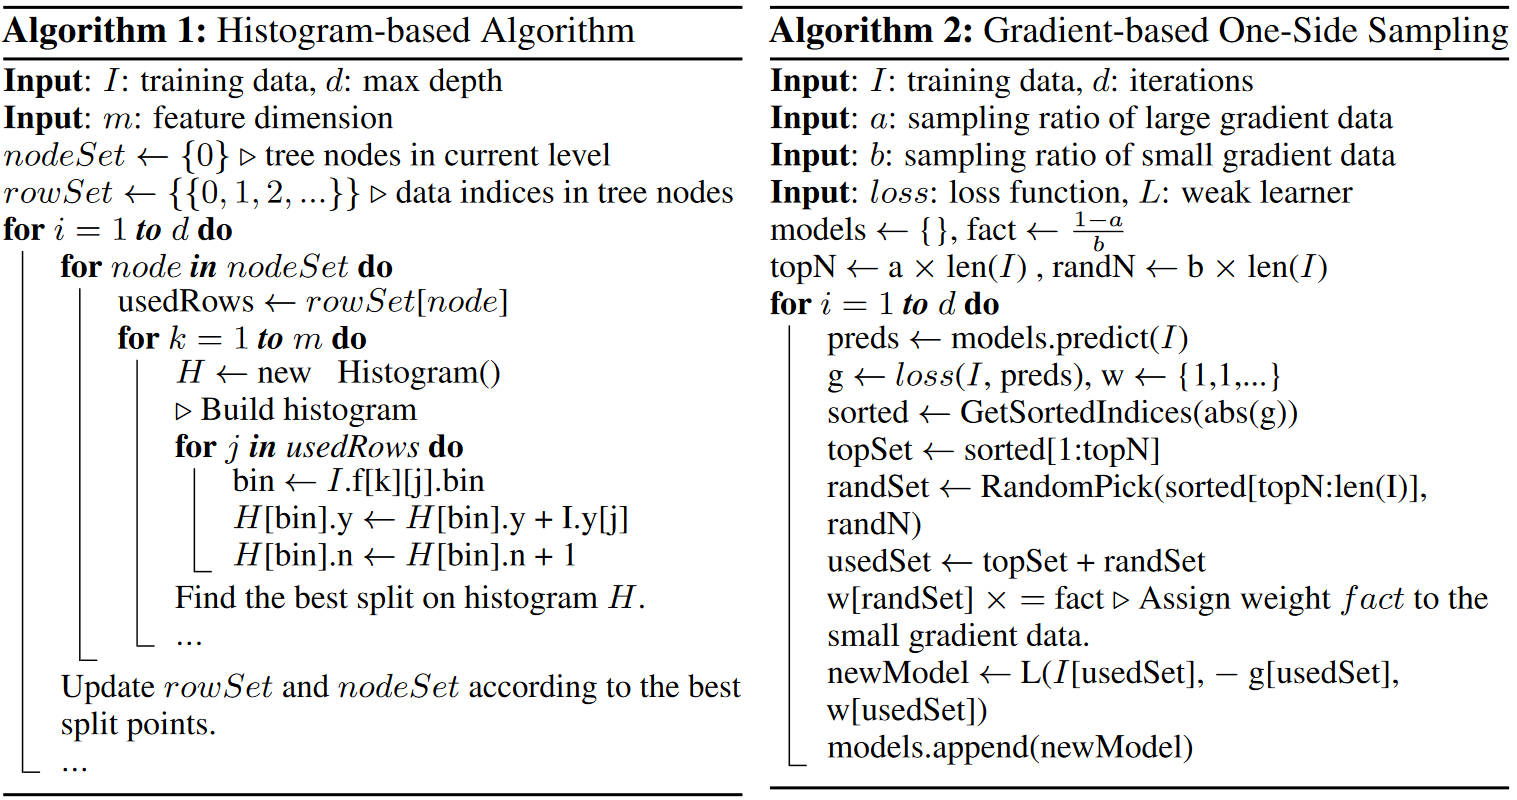
\includegraphics[width=\textwidth]{pics/goss.jpg}
	\caption{Histogram-based Algorithm 和 Gradient-based One-Side Sampling}
	\label{fig:goss}
\end{figure}

基于梯度的单边采样, 在尽量保证效果的基础上过滤掉一部分梯度较小的样本. 因此重点是基于什么来对样本进行过滤? 如果有样本权重, 那么根据权重来采样是可以的, 但很多场景下是没有的. 从 GOSS 的名字也可以看出, lgb 中是\textbf{基于梯度来采样}的. 为什么可以这样呢? lgb 作为 GBDT 的一种实现, 本身也是基于梯度的. 因此如果样本的梯度较小则说明其以及可以被很好分类了, 那么其就是个 \textit{easy sample}, 对于哪些梯度大的则是 \textit{hard sample}. 所以, lgb 中以样本梯度的绝对值作为采样的依据. 但是采样后可能会改变数据的分布, 因此, GOSS 在采样后还有一个缩放的操作. 具体的采样过程其是很简单:
\begin{myitemize}	
	\item 基于已有的模型 (即前面已经训练好的树) 计算每个样本的梯度;
	
	\item 按照梯度绝对值大小对样本进行排序;
	
	\item 取前 $a (\in (0, 1))$ 的数据作为大梯度的样本, 保留下来;
	
	\item 在剩下的 $1-a$ 的样本中随机选择 $b (\in (0, 1))$ 的样本保留下来, 并对这些样本的梯度进行缩放, 乘以 $\frac{1 - a}{b}$;
	
	\item 上两步保留的样本作为这一轮的训练数据;
\end{myitemize}

注意, 根据采样比例计算采样样本数时, 都是相对总样本而言(从 Fig.\ref{fig:goss} 中的 \textit{Gradient-based One-Side Sampling} 可以看出)! 为什么要对小梯度中采样到的样本的梯度进行 $\frac{1 - a}{b}$ 的缩放呢? 

假设小梯度的样本的平均梯度是 $\mu$, 则采样前梯度的总量是 $\text{len}(I) \cdot (1-a) \cdot \mu$, 那么采样后的梯度总量是 $\text{len}(I) \cdot b \cdot \mu$. 为了保持梯度总量不变, 即 $\text{len}(I) \cdot (1-a) \cdot \mu = \text{len}(I) \cdot b \cdot \mu \cdot x$, 显然 $x = \frac{1 - a}{b}$, $x$ 就是缩放系数.

\paragraph{EFB}
互斥特征绑定. 高维的特征大多是很稀疏的, 如果能在牺牲一点点效果的条件下降低特征的维数就可以大大提高性能. 在稀疏的数据中, 存在一些\textbf{互斥的特征}: 这些特征基本上不会同时取非零值. EFB 将这些互斥的特征进行组合作为一个单一的特征, 一次来减少特征的数量. 如何做到呢? EFB 分成两步走: 1) 哪些特征应该被划分到一个 \textit{bundle}; 2) 如何组合 \textit{bundle} 中的特征.

\begin{figure}[h]
	\centering
	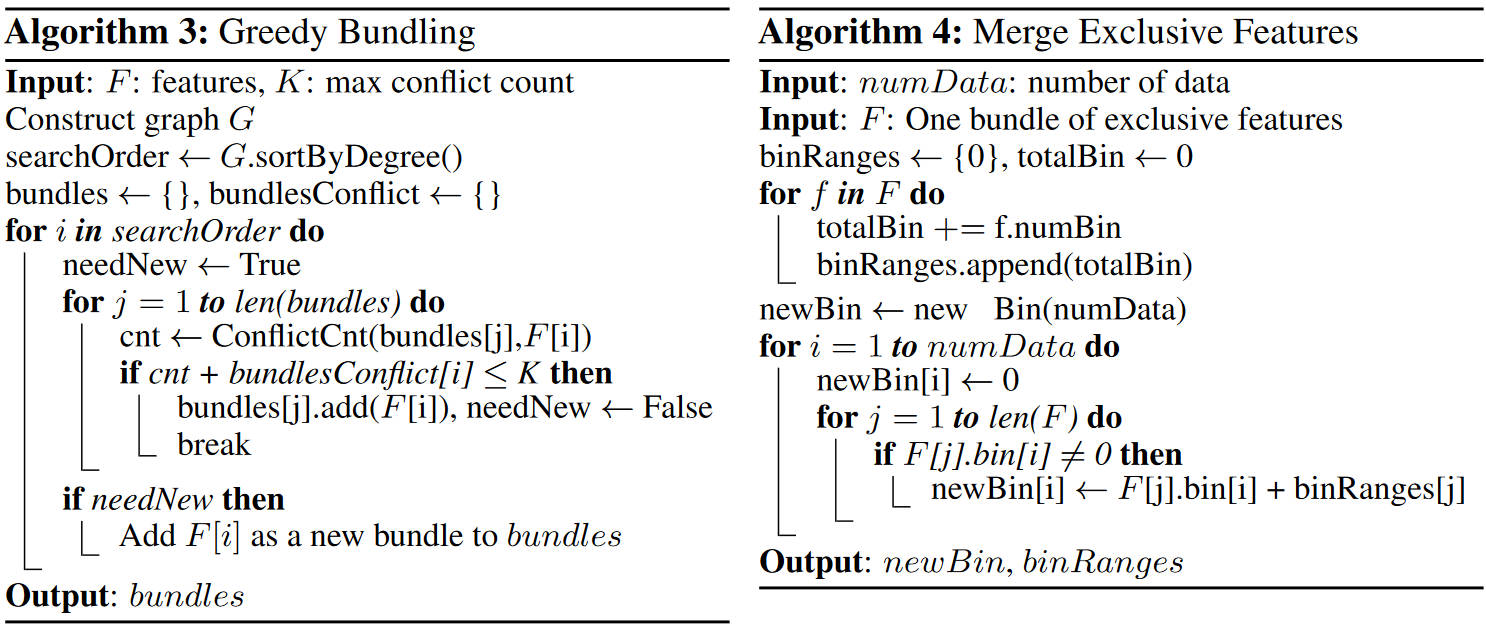
\includegraphics[width=\textwidth]{pics/efb.jpg}
	\caption{EFB 中的两个算法: 构建 \textit{bundle} 和 组合 \textit{bundle} 中的特征}
	\label{fig:efb}
\end{figure}

\subparagraph{Greedy Bundling}
直接对特征进行组合的话将会是一个 NP-hard 的问题, 因此 lgb 将该问题转化为 graph coloring 问题: 将每一个特征视作一个结点, 如果两个特征(结点)不满足互斥的条件则存在边. 再采用贪心的算法来对构建的图进行染色, 最终得到原特征集合的划分, 如 Fig.\ref{fig:efb} 中的 \textit{Greedy Bundling} 所示. 每个 \textit{bundle} 中就是互斥的特征集合. EFB 中并不是严格的互斥, 从算法的伪代码中也可以看到, 冲突次数小于等于 $K$ 是视为互斥的. lgb 中还给出了冲突率和 \textit{accuracy} 的影响的证明. 

\subparagraph{Merge Exclusive Features}
如何把一个 \textit{bundle} 的特征合并为一个特征呢? 一个关键: \textbf{可以从合并后的特征识别处原始特征的值}, 即尽可能降低信息的损失. lgb 中是引入了 \textit{offset} 来帮助区分该值是来源于 \textit{bundle} 中的哪个特征. 例如一个 \textit{bundle} 中的两个特征 $A, B$. 其中 $A$ 的取值范围是 $[0, 10)$, $B$ 的取值范围是 $[0, 20)$. 可以对 $B$ 的取值加上一个值为 10 的 \textit{offset}, 则合并后的特征的取值范围是 $[0, 30)$. 


当然, 除了以上两点, lgb 中还有一些其他改变, 比如改用 \textit{leaf-wise} 的生长策略, 而不是 \textit{level-wise}. 

\textcolor{red}{\textbf{注意}}: 其实关于 lgb 还有一些疑惑, lgb 是否用到了损失函数的二阶导; EFB 之后是怎么进行分裂的.

一些参考资料: \href{https://mp.weixin.qq.com/s/XxFHmxV4_iDq8ksFuZM02w}{LightGBM源码阅读+理论分析(处理特征类别, 缺省值的实现细节)}.

\subsubsection{Core Parameters}
主要参考\href{https://lightgbm.readthedocs.io/en/latest/Parameters.html#}{这里}.
\paragraph{任务相关的参数}
这一部分的参数主要是由你要做什么任务来确定的.
\begin{myitemize}
	\item \mintinline{python}{task} : 指示任务的阶段, 如训练, 预测, 重新拟合等;
	
	\item \mintinline{python}{objective} : 指示要学习的任务的类型, 如回归, 二分类, 多分类, 排序等;
	
	\item \mintinline{python}{boosting} : 使用何种基学习器;
	
	\item \mintinline{python}{num_iterations} : 迭代的次数;
	
	\item \mintinline{python}{num_class} : 类别的数量, 只用在多分类中;
	
	\item \mintinline{python}{learning_rate} : 学习率, 即 xgboost 论文中的 shrinkage rate, 这个参数即控制每一轮学习的幅度, 留一部分学习空间给后来的学习器, 避免一个学习器的效果对目标值起主导作用;
	
	\item \mintinline{python}{tree_learner} : 这个参数控制了并行的粒度;
	
	\item \mintinline{python}{device_type} : 在什么设备上学习, 即 cpu, gpu, cuda, cuda\_exp.
\end{myitemize}

\paragraph{基学习器的参数}
LightGBM 本身也是一种集成学习的方式, 因此关于基学习器也有很多重要的参数, 这些也是调参过程中的主要对象.
\begin{myitemize}
	\item \mintinline{python}{num_leaves} : 树中最大叶子数. 注意与 xgboost 树生长的形式不同, lgb 是按照逐个叶子分裂的. 从树模型的复杂度定义来看, 这个参数影响了模型的复杂度, 因此如果该值过大则容易引发\textbf{过拟合}. 通常, 在相同的叶子数下, 逐层生长的树比逐叶子生长的树要深不少;
	
	\item \mintinline{python}{min_data_in_leaf} : 叶子结点中最少有多少样本. 很显然, 如果这个值设置的比较大, 那么树中的叶子数会比较小, 也能抑制树的生长, 因此可能会引发\textbf{欠拟合};
	
	\item \mintinline{python}{max_depth} : 一棵树的最大高度;
	
	
\end{myitemize}

\paragraph{学习过程中的参数}
这些参数主要是控制学习过程中的行为, 如采样等.
\begin{myitemize}
	\item \mintinline{python}{bagging_freq} : lgb 中有一个 bagging 的概念 (\textbf{\textcolor{red}{还不是很了解}}), 这个参数控制了 bagging 的频率;
	
	\item \mintinline{python}{bagging_fraction} : 如果进行 bagging, 则每次 bagging 时会对数据进行采样, 用采样到的数据进行训练. 这个参数则控制了采样的比例;
	
	\item \mintinline{python}{pos_bagging_fraction / neg_bagging_fraction} : 只在二分类中使用, 控制 bagging 采样时正负样本的比例;
	
	\item \mintinline{python}{min_data_in_leaf} : 树的叶子节点中至少有多少样本. 这个值是根据海森矩阵估计的, 因此在实际中叶子结点中的样本数可能会少于设定的值;
	
	\item \mintinline{python}{feature_fraction} : 列采样的比例. 这个采样是在构建每棵树的时候进行的. 类似的还有 \mintinline{python}{feature_fraction_bynode}, 在每个节点分裂时采样的比例;
	
	
	\item \mintinline{python}{force_col_wise / force_row_wise} : 直方图建立的方式, 逐列或逐行. 这个还不太清楚是啥意思, 可能要看看论文;
	
	\item \mintinline{python}{lambda_l1, lambda_l2} : l1, l2 正则项的系数;
	
	\item 
\end{myitemize}

\paragraph{Dataset 相关的参数}
\begin{myitemize}
	\item \mintinline{python}{max_bin} : 特征分桶时最多可以分多少桶, 也可以通过 \mintinline{python}{max_bin_by_feature} 来指定每个特征最多可以分多少桶;
	
	\item \mintinline{python}{min_data_in_bin} : 一个桶里至少有几个样本;
	
	\item \mintinline{python}{use_missing} : 是否处理缺失值;
	
	\item \mintinline{python}{feature_pre_filtr} : 是否在学习前先过滤一遍特征. lgb 会忽略那些不能用于分裂的特征, 如特征值全都相同的特征, 不能满足 \mintinline{python}{min_data_in_leaf} 的特征;
\end{myitemize}

简单地梳理了一下 LightGBM 的参数, 可以明显地感觉到 lgb 的参数要比 xgb 多, 划分地也更精细.

\subsubsection{调参}
调参, 一般来说是为了获得更好的效果, 但也可以是为了保证一定效果地条件下获得更快的运行速度. 出于不同地目的, 要调整的参数也是不一样的. 这里还是先以效果为目标来介绍调参的过程.
\begin{myenumerate}
	\item 先使用大一些的学习率, 调节 \mintinline{python}{n_iterations}, 即找到大概需要多少轮的增强可以达到较好的效果. 这里先从全局的角度来调. 不涉及每一轮的学习过程中的参数;
	
	\item 接下来调关于每轮学习过程中的参数, 主要是基学习器相关的一些参数. 如 \mintinline[breaklines]{python}{max_depth, num_leaves, min_data_in_leaf, min_data_in_bin, min_sum_hessian_in_leaf, pos_bagging_fraction, neg_bagging_fraction, bagging_freq, bagging_fraction}. 当然, 这几个参数也可以分成几组来调, 可以按照参数的重要性来调节;	
	
	\item 关于正则化项的参数, 如 \mintinline{python}{lambda_l1, lambda_l2, min_gain_to_split, drop_rate} 等;
	
	\item 降低学习率, 并增大迭代的轮数;
	
	\item 可以选择重复上述过程.
\end{myenumerate}
其实, 调参并不能带来大幅的提升, 主要还是看特征工程、模型集成等.

\subsubsection{类别特征的处理}
LightGBM 中引入了对 类别特征的支持, 对于基数较大的类别特征而言, 如果将其展开为 one-hot, 是会有一些坏处的, 例如: 1) 大大增加特征的维数, 空间效率降低; 2) one-hot 展开后, 每个类别上的样本数可能会很少, 分列时是按照 ovr 的形式分裂的, 因为样本过少可能会存在估计不准的情况. lgb 中并不需要将类别特征展开为 one-hot, 可以直接对类别特征进行划分, 按照 many-vs-many 的形式进行划分. 那怎么将一个类别特征的取值划分成两部分呢?

这一过程分成两步:
\begin{enumerate}
	\item 离散特征建立直方图. 众所周知, lgb 中使用了直方图算法来对特征进行分桶, 在这些桶中寻找分裂点. 显然, 也会为离散特征建立直方图, 直方图的每个 \textit{bin} 中保存的是样本的一阶和二阶导数. 当然并不是为每个离散值建立一个 \textit{bin}, 对于那些出现次数过少的离散值则会被过滤掉 (多少算少呢? 这个是可以通过参数 \mintinline{python}{min_data_in_bin} 来指定的);
	
	\item 计算分裂的阈值. 先检查这个时候该特征下 \textit{bin} 的数量, 若其小于一定的数量 (由参数 \mintinline{python}{max_cat_to_onehot} 指定) 时则按照 one-hot 的形式对待, 即 ovr 的形式. 当 \textit{bin} 较多时, 则会根据每个 \textit{bin} 的 \mintinline{python}{sum(gradient) / sum(hessian) + reg} 值来对该特征下的 \textit{bins} 进行排序, 然后遍历每个桶找到最优的切分点.
\end{enumerate}

参考: \href{https://lightgbm.readthedocs.io/en/latest/Features.html#optimal-split-for-categorical-features}{Optimal Split for Categorical Features}.


\clearpage
\part{Deep Learning}
{\noindent}	 \rule[-10pt]{17.5cm}{0.5em}\\ 
\section{Basics}
\subsection{BGD, SGD, MBGD}
神经网络的训练过程, 可以看作目标函数的优化过程, 在优化过程中对模型的参数进行更新, 使目标函数逐步收敛到一个最优的状态. 参数优化有多种方法, 目前主要是基于迭代的过程, 如梯度下降、牛顿法等. 其中梯度下降已经霸榜多年. 目前主要有以下三种梯度下降方法: 
\begin{myitemize}
	\item BGD, Batch  Gradient Descent, 批量梯度下降. 每次计算梯度时使用全量样本. 优点: 
	\begin{myitemize}
		\item 所有样本都参与了梯度的计算, 异常样本带来的影响更小, 训练过程更稳定
		\item 收敛速度快
	\end{myitemize}
	缺点也很明显, 因为使用到了所有样本, 故计算耗时更长, 且要将数据全部加载, 对资源要求更高, 且有可能收敛到局部最优. 
	
	\item SGD, Stochastic Gradient Descent, 随机梯度下降. 每次计算梯度时只使用一个样本, 通常会对全量数据进行打乱. 优点: 
	\begin{myitemize}
		\item 参数更新频次高, 速度快. (但从另一个角度来看, 单独计算每个样本的梯度或许更耗时)
		\item 可以在线优化
		\item 每次使用一个样本的随机性可能会帮助跳出局部最优
	\end{myitemize}
	缺点: 每次只是用一个样本, 会放大一场样本的影响, 导致训练过程不稳定. 
	
	\item MBGD, Mini-Batch Gradient Descent, 小批量梯度下降. 每次使用一部分数据计算梯度, 一次通常将全量数据划分成多个batch, 与SGD类似, 也会对全量数据进行打乱. 优点: 
	\begin{myitemize}
		\item 对比BGD, 速度更快, 对资源要求更低;对比SGD, 振荡现象没有那么明显, 比SGD会更稳定
		\item 能够一定程度避免异常样本的干扰
	\end{myitemize}
	缺点: 需要考虑学习率的衰减, 以及选择合适的batch size, 且与BGD相比存在一定程度的振荡. 
\end{myitemize}
参考资料: \href{https://lumingdong.cn/summary-of-gradient-descent-algorithm.html#%E6%A2%AF%E5%BA%A6%E4%B8%8B%E9%99%8D%E7%AE%97%E6%B3%95%E7%9A%84%E4%B8%89%E4%B8%AA%E5%8F%98%E7%A7%8D}{梯度下降算法的三个变种}. 

\subsection{Normalization}
\subsubsection{Batch Normalization}
在神经网络中, 前一层的输出会成为后一层的输入. 当前面层的参数更新后, 其输出的分布也会随之改变, 经过层层的叠加, 越往后的变化越大. 为了拟合这些数据, 深层的参数需要不断适应变化的数据, 导致模型的\textbf{收敛速度很慢}. 这里的分布指的是一层里每个神经元的分布. 这种分布不一致做 \textbf{Internal Convariate Shift}(内部协变量偏移). 对于一个神经元, 其取值分布会逐渐偏移, 例如偏移至激活函数的饱和区, 即梯度很小. 

一个比较直观的方式就是对每一层的输出进行标准化. Batch Normalization 在 mini-batch 的基础上对每个神经元进行标准化, 即对每个特征进行标准化. 具体操作为: 每一层的输入为一个 mini-batch, 通过这个批次来估算每一维的均值和方差, 然后对每一维进行标准化, 除此之外, BN 中还对标准化后的特征进行了线性变化. 
$$
\begin{array}{rlr|}
	\hline \text { Input: } & \text { Values of } x \text { over a mini-batch: } \mathcal{B}=\left\{x_{1 \ldots m}\right\} \\
	& \text { Parameters to be learned: } \gamma, \beta & \\
	\text { Output: } & \left\{y_{i}=\operatorname{BN}_{\gamma, \beta}\left(x_{i}\right)\right\} & \\
	\mu_{\mathcal{B}} & \leftarrow \frac{1}{m} \sum_{i=1}^{m} x_{i} & \multicolumn{1}{l|}{\text { // mini-batch mean }} \\
	\sigma_{\mathcal{B}}^{2} & \leftarrow \frac{1}{m} \sum_{i=1}^{m}\left(x_{i}-\mu_{\mathcal{B}}\right)^{2} & \text { // mini-batch variance } \\
	\widehat{x}_{i} & \leftarrow \frac{x_{i}-\mu_{\mathcal{B}}}{\sqrt{\sigma_{\mathcal{B}}^{2}+\epsilon}} & \text { // normalize } \\
	y_{i} & \leftarrow \gamma \widehat{x}_{i}+\beta \equiv \mathrm{BN}_{\gamma, \beta}\left(x_{i}\right) & \text { // scale and shift }
\end{array}
$$
注意上面公式中是以一个特征维度为例子, 对于其他维也是一样的, 其中的 $\gamma, \beta$ 都是需要学习的参数, 即每个神经元会多出来两个参数来学习. 上述过程是在针对训练而言的, 但是在推断时该怎么办呢?对于测试数据, 依然会进行标准化($\gamma, \beta$ 是在训练时学习好的, 所以推断时是会被固定的), 但是其均值和标准差就不是通过批次数据来计算的, 而是这样: 
$$
\begin{aligned}
	\mathrm{E}[x] & \leftarrow \mathrm{E}_{\mathcal{B}}\left[\mu_{\mathcal{B}}\right] \\
	\operatorname{Var}[x] & \leftarrow \frac{m}{m-1} \mathrm{E}_{\mathcal{B}}\left[\sigma_{\mathcal{B}}^{2}\right]
\end{aligned}
$$
那么测试数据的标准化就是这样的: 
$$
\widehat{x}=\frac{x-\mathrm{E}[x]}{\sqrt{\operatorname{Var}[x]+\epsilon}}
$$
\textbf{为什么标准化后还要进行线性变换呢?}如果只是进行标准化后, 其很有可能落在激活函数的线性区域, 例如 sigmoid 激活函数, 经过标准化后基本会落在 0 左右, 而这一块区域基本是线性的, 而达不到激活函数的非线性的功能, 因此对齐进行了缩放和偏置, 使其能够落在激活函数的非线性区域, 由于 $\gamma, \beta$ 是学习得到的, 因此也能满足其落在线性区的需求. 这样做的一个目的就是: 保障每一层的表征能力. 

有一些观点认为 BN 有防止过拟合的作用, 给出的解释是: BN 将输入拉到了同一个分布, 且保证了输入不会都落到激活函数的饱和区, 可以使得参数的更新更加平滑, 也就达到了防止过拟合的作用. 


实际情况在进行BN时, 可能是在通过激活函数之前进行 BN 或者在通过激活函数后再进行BN. \textbf{通常是在激活函数之前进行 BN}, 因为当输入较大时, 通常激活函数的变化都较小, 梯度变化不明显, 故在激活函数之间就对数据进行BN, 使其分布尽量稳定. 

BN 的一些缺点: 
\begin{itemize}
	\item 需要较大的batch以体现整体数据分布, 要求 bath 的分布尽量与总体分布相近;
	\item 训练阶段需要保存每个batch的均值和方差, 以求出整体均值和方差在infrence阶段使用;
	\item 不适用于可变长序列的训练, 如RNN. 
\end{itemize}

\subsubsection{Layer Normalization}
既然已经有了 BN, 怎么还来了 LN 呢?参看 BN 的缺点, 其中很重要的一点就是不适用于处理序列数据的网络, 序列数据的格式通常为 $(batch\_size, seq\_len, emb\_dim)$, 但是$seq\_len$ 并不都是相同的. 如果对序列数据进行 BN, 则需要计算每个 $time\ step$ 上每个特征的均值和方差, 但是由于序列的长度是不一致的, 若遇到了没有在训练集中出现过的序列长度则无法对超出的 $time\ step$ 做 BN 了. 

与 BN 类似, LN 也是进行标准化后再进行线性变化. 不同点在于 LN 的标准化是针对层而言的, 而 BN 的标准化是针对神经元而言的. 具体做法: LN 计算层中所有神经元的均值与方差, 对于一个 batch 而言, 则会计算出 $(batch\_size, seq\_len)$ 个均值和方差, 即序列中每个元素(维度为 $emb\_dim$ 的向量)一对均值和方差, 然后对同一层使用相同的均值和方差做标准化后进行线性变化即可. 
$$
\mu^{l}=\frac{1}{H} \sum_{i=1}^{H} a_{i}^{l} \quad \sigma^{l}=\sqrt{\frac{1}{H} \sum_{i=1}^{H}\left(a_{i}^{l}-\mu^{l}\right)^{2}}
$$
其中 $a_i^l$ 就是第 $l$ 层的第 $i$ 个神经元, $H$ 是隐层的单元数. 可以看到, 计算的过程中不用考虑 batch 的大小, 因此 batch 的大小和选择对 LN 是没有影响的. 进行缩放时则与 BN 是一致的, 每个神经元都有单独的缩放系数和偏置. 因为不受 batch 中其他样本的影响, 因此使用 LN 时不需要保存训练过程中各个 batch 的均值和方差, 且训练过程和推断过程 LN 的操作是一致的. 

\subsection{Dropout}
Dropout 即丢弃, 是神经网络中一种正则化的手段: 在神经网络模型做训练时, 让网络中某些神经元随机失活——也就是不参与训练. 换个角度理解一下这个操作背后的含义: Dropout使得每批训练数据进入神经网络时, 神经网络的构型都不同, 即每批训练数据训练的网络结构都不同. 而做预测Dropout是关闭的状态, 代表着\textbf{做预测时是所有训练时结构不同的神经网络一起做的最后的预测, 整个过程就是多个不同神经网络最后投票做决定给出预测值}. 其实可以看到这和随机森林的 \textbf{bagging} 很像了. 

参考 PyTorch 中关于 Dropout 的实现: \ref{nn_dropout}. 

\subsection{Model Collapse}
模型坍塌, 很形象啊, 就是模型出现了一个漏洞, 不管你输入什么东西都会漏进这个洞里. 

这个主要出现在GAN的模型中. GAN通过生成器G和判别器D来使G捕捉到真实数据的分布. 在训练GAN模型时会出现model collapse的现象, 即G只捕捉到了真实数据的部分分布. 为什么会这样呢?简单的介绍一下: 当G捕捉到了真实数据的部分分布后, 被D识破了, 于是G就改变, 从某个分布跳到了另外的分布, 并且抛弃了原来的分布, 于是就成了“猫鼠游戏”, D一直追着G跑, G最终并没有完全捕捉到真实数据的分布. 参考: \href{https://blog.csdn.net/SPARKKKK/article/details/72598041}{GAN——ModeCollapse}. 


\subsection{关于CNN的一点理解}
于DNN相比, CNN有两个特点: 1)局部感知;2)权值共享. 

局部感知. 在CNN中每个Feature map中的一个值只于上一层的Feature map的一小部分有关. 如果将CNN展开成DNN的形式, 则一层中的一个神经元的输入只是上一层的某几个神经元. 与全连接不同, 全连接将上一层的所有信息作为输入, 捕捉整体的信息. 但局部感知以某个区域内的信息作为输入, 捕获上一层数据中存在的局部信息 --- 特定的模式. 

权值共享. CNN中的每一个filter都可以得到一个Feature map, 同一个Feature map中的元素之间通过同一个filter卷积得到. 或者说, 同一层的神经元由一个filter产生, 共享一套参数. 
见Fig.\ref{fig:share_weight}. 图来源于李宏毅老师的ppt. 有一点需要注意, CNN模型的输入图像可能是单通道的也可能是三通道的, 此时\textbf{每个filter不仅由长和宽还有深度}, filter的深度与图像的通道数是相等的, 所以一般来说有多少个filter就有多少个Feature map. 

\begin{figure}[h]
	\centering
	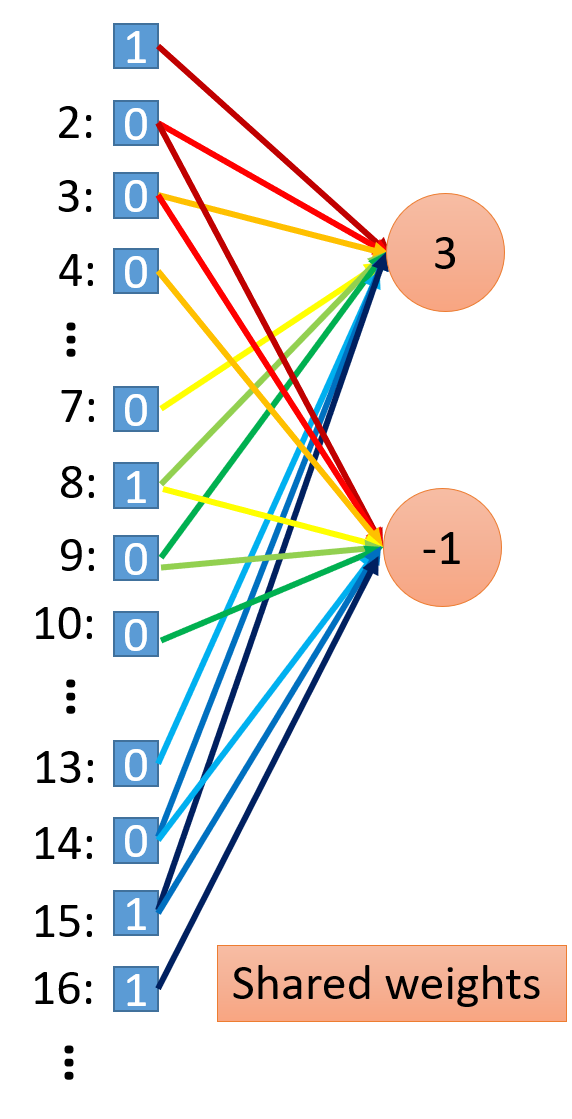
\includegraphics[width=.3\textwidth]{pics/share_weight.png}
	\caption{CNN的权值共享}
	\label{fig:share_weight}
\end{figure}

CNN的应用非常广泛, 不仅是图像, 在Speech、NLP等很多领域都有非常多的应用. 在决定是否要使用基于CNN的模型时, 需要考虑: 1)数据中存在一些较小的模式, 这些模式经常出现在数据中 --- 对用卷积核;2)模式与整个数据相比比较小, 更大的语义信息是由很多小的模式组成的;3)进行pooling时不会破坏数据本来的含义. 

在探索CNN到底学习到了什么的时候, 可以在训练好模型后, 通过不断优化输入的数据, 来检验是什么样的输入使得基于CNN的模型中的神经元能够得到最大的激活 --- 什么样的输入使神经元最兴奋. 这些主要涉及到对CNN的解释和可视化. 

\subsection{深度学习中常见的参数初始化方法}
深度学习依靠大量的数据进行学习能够达到很好的效果, 但是这其中依靠的是大量的参数, 学习就是为这些参数找到合适的值. 因此, 如果一开始我们就能给这些参数设置一个比较好的值, 那么学习也就省力了, 这也就是如何初始化的问题了. 

\subsubsection{从正态分布中采样}
或许直接将参数初始化为 0 也能进行学习, 但是容易存在一些问题: 学习过程缓慢, 难以收敛, 学习效果不好, 为什么呢?如果参数全为 0, 则计算的损失可能会很小, 能够提供的梯度值也会很小或者根本就等于 0, 这对于依靠梯度更新参数的方法来说是很致命的. 因此, 与全 0 相比, 随机初始化反而是一个不错的选择, 至少不会让梯度为 0. 

\subsubsection{Glorot initialization}
但是呢, 从正态分布中采样也不是一个很好的方法, 为什么呢?将设我们从 $\mathcal{N}(\mu, \sigma^2)$ 中采样权重, 参数的方差会影响隐层的线性变换后的方差, 进而影响隐层输出的方差, 这会直接影响梯度的计算, 如以 sigmoid 为激活函数时, 则可能落在平坦的区域 --- 也就是可能会出现梯度向后传着传着就没了或者就变得很大了. 

因此一个好的初始化应该满足: 各层的值(线性变换后的值、激活后的值)应该有相似的方差. 为了满足前向传播时各隐层的输出值有相似的方差, 以及在反向传播时, 梯度也具有相似的方差, 我们可以推导出参数应该又怎样的方差, 这其中涉及到一些数学推导, 暂时不展开. 结论就是, 为了前向的稳定, 参数的方差应该是 $\frac{1}{f_{in}}$, 为了反向传播的稳定, 参数的方差应该为 $\frac{1}{f_{out}}$, 其中 $\boldsymbol{W}^{fan_{in} \times fan_{out}}$. 那这里有两个方差怎么办: 取平均, 即 $Var(\boldsymbol{W}) = \frac{1}{ \frac{fan_{in} + fan_{out}}{2}}  = \frac{2}{fan_{in} + fan_{out}}$. 因此如果我们从正太分布中采样, 则这个正太分布的方差应该等于 $\frac{2}{fan_{in} + fan_{out}}$, 均值应该等于 0, 为啥呢?在推导过程中利用了方差的一些性质, 要求均值为 0. 如果从均匀分布 $U(a, b)$ 中采样呢?同样需要满足 0 均值, 即 $a + b = 0$, 那等于多少呢?因为均匀分布的方差为 $\frac{(b - a)^2}{12}$, 且 $a = -b$, 因此可以解得 $b = \sqrt{\frac{6}{fan_{in} + fan_{out}}}$. 

上述方法就是Xavier初始化方法(又称Glorot初始化). 当然, 初始化方法还要考虑激活函数的影响, Glorot 主要用于输出均值为 0 的激活函数, 如 tanh. 

\subsubsection{He 初始化}
如果使用 ReLu 作为激活函数, 上述的 Glorot 可能就不是那么好了, 为什么呢?考虑 $ReLu(x) = max(0, x)$, 将隐层的输出近一半置为 0, 且 ReLu 的输出均值不为 0, 不满足 Glorot 推导过程中的一些条件. 为了满足各层的值方差就近似, He 初始化对权重的方差变为了 Glorot 中的两倍, 为什么呢?因为 ReLu 将一般元素的值置零相当于减少了一半方差. He 初始化没有同时使用 $fan_{in}, fan_{out}$, 而只使用了其中一个, 实验表明这已经足够了. 因此, 使用 He 初始化时, 正态分布的方差为 $\frac{2}{fan_{in}}$, 均匀分布的的 b 为 $\sqrt{\frac{6}{fan_{in}}}$. 

关于推导的一些参考: \href{https://intoli.com/blog/neural-network-initialization/}{UNDERSTANDING NEURAL NETWORK WEIGHT INITIALIZATION}、\href{https://mnsgrg.com/2017/12/21/xavier-initialization/}{Xavier Initialization}(不同激活函数下的 Glorot 初始化推导). 


\subsection{DL中的不可微操作}

\subsection{Global Max Pooling}

\subsection{Attention机制与CNN}

\subsection{Batch Size与Learning Rate}
模型训练过程中, \textbf{Batch Size}和\textbf{Learning Rate}是两个不可不调的参数. 


\subsection{深度学习的梯度下降优化算法}
这里按照 PyTorch 里的优化器来进行介绍. 
\subsubsection{SGD}
\href{https://pytorch.org/docs/stable/generated/torch.optim.SGD.html#torch.optim.SGD}{SGD}(stochastic gradient descent), 就是常说的随机梯度下降, 当然在 PyTorch 的实现中, 可以加入一些额外的操作, 如: 权重衰减、动量(上一步的梯度呈指数加权来影响当前梯度). SGD 的计算过程如 Fig.\ref{fig:sgd} 所示. 

\begin{figure}[h]
	\centering
	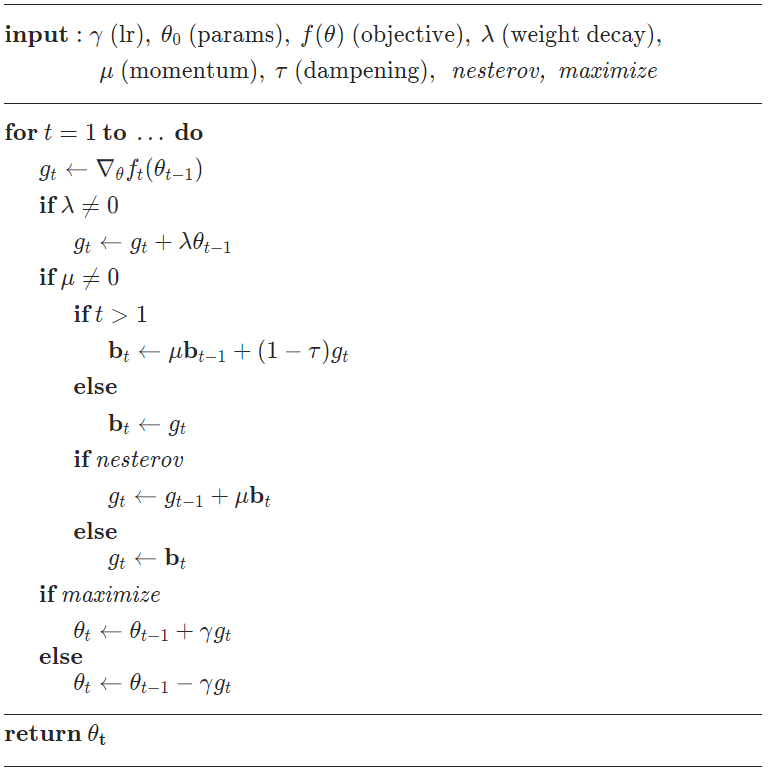
\includegraphics[width=0.6\textwidth]{pics/sgd.png}
	\caption{SGD 计算过程(\href{https://pytorch.org/docs/stable/generated/torch.optim.SGD.html#torch.optim.SGD}{来源})}
	\label{fig:sgd}
\end{figure}

SGD 的特点: 
\begin{itemize}
	\item 朴素的 SGD 最大的缺点是下降速度慢, 而且可能会在沟壑的两边持续震荡, 停留在一个局部最优点;
	
	\item 为了解决朴素 SGD 中的振荡现象, 可以加入动量;
	
	\item 对于稀疏数据集, 对所有参数使用相同的学习率是不太合适的, 每个参数更新的步长与特征的稀疏程度有关;
\end{itemize}

\subsubsection{AdaGrad}
即 Adaptive Gradient, 自适应梯度. 该算法通过记录迭代过程中梯度的信息来自动地调整学习率. 可以实现针对不同的参数自动调节学习率的大小. 其计算方式:

$$
w^{t+1} \leftarrow w^t - \frac{\eta}{\sqrt{\sum_{i=0}^t (g^i)^2}} \odot g^t
$$

可以看出, 随着迭代, 学习率是\textbf{单调递减}的, 且对于梯度较大的参数其更细你的步伐也更大. 其缺点为: 1) 从训练开始时累积平方梯度值会越来越大, 会导致学习率过早和过量的减少, 从而导致迭代后期收敛及其缓慢; 2) 需要手动设置全局学习率. 

\subsubsection{RMSProp}
即 Root Mean Square Prop, 该算法是 AdaGrad 的一种改进, 区别在于梯度累计的方式不同, 在 AdaGrad 中为累加梯度的平方, RMSProp 中则是引入了一个衰减系数来累加:

$$
r \leftarrow \rho r + (1 - \rho) g \odot g
$$
其中 $r$ 就是梯度累积量, 梯度更新方式与 AdaGrad 一样:

$$
w^{t+1} \leftarrow w^t - \frac{\eta}{\sqrt{r}} \odot g^t
$$

由于 $r$ 参考了历史的梯度信息, 因此在更新的过程中更稳定.

\subsubsection{AdaDelta}
AdaDelta 也是针对 AdaGrad 的一种改进. 与 RMWProp 不同, AdaDelta 不需要设置一个初始的学习率. 其计算过程如 Fig.\ref{fig:adadelta} 所示.

\begin{figure}[h]
	\centering
	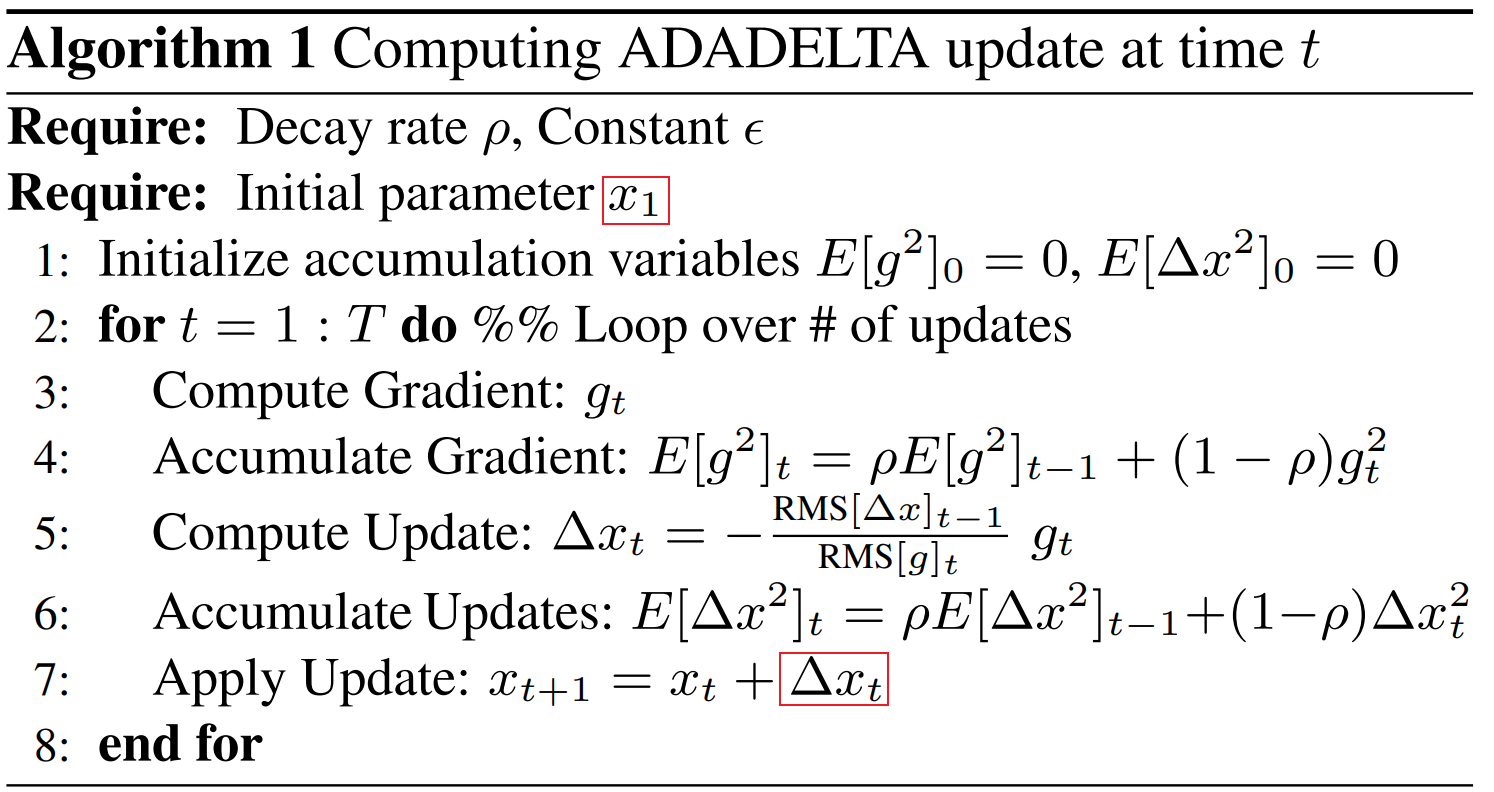
\includegraphics[width=0.8\textwidth]{pics/adadelta.png}
	\caption{AdaDelta 计算过程}
	\label{fig:adadelta}
\end{figure}

参数的更新量 $\Delta x_t$ (AdaDelta 中的 Delta 应该就是指 $\Delta x$)并不是通过学习率乘以梯度得到的, 而是一个指数加权平均的量. 与 RMSProp 相比, AdaDelta 相当于用上一步参数更新量的均方根近似学习率 ($\Delta x_t = -\frac{\text{RMS}[\Delta x]_{t-1}}{\text{RMS}[g]_t} g_t$). 

AdaDelta \textbf{特点}: 1) 不需要设置初始的学习率, 但是在一些深度学习框架中 (如 pytorch), 可以看到所实现的 AdaDelta 优化器还有学习率这个参数, 但是这个学习率是针对 $\Delta x$ 所做的缩放, 其取值也一般比较大; 2) 训练的早期和中期收敛速度快 (\textcolor{red}{从\href{https://arxiv.org/pdf/1212.5701.pdf}{论文}来看, $\Delta x$ 的更新类似于牛顿迭代, 使用了近似二阶信息, 所以收敛快}), 但是后期容易在局部最小值附近抖动.

\subsubsection{Adam}
Adam\cite{kingma2015adam} 结合 AdaGrad 和 RMSProp 两种优化算法的优点, 对梯度的一阶矩估计(First Moment  Estimation, 即梯度的均值)和二阶矩估计(Second Moment Estimation, 即梯度的未中心化的方差)进行综合考虑, 计算出更新步长. Adam 的计算过程如 Fig.\ref{fig:adam} 所示. 

\begin{figure}[h]
	\centering
	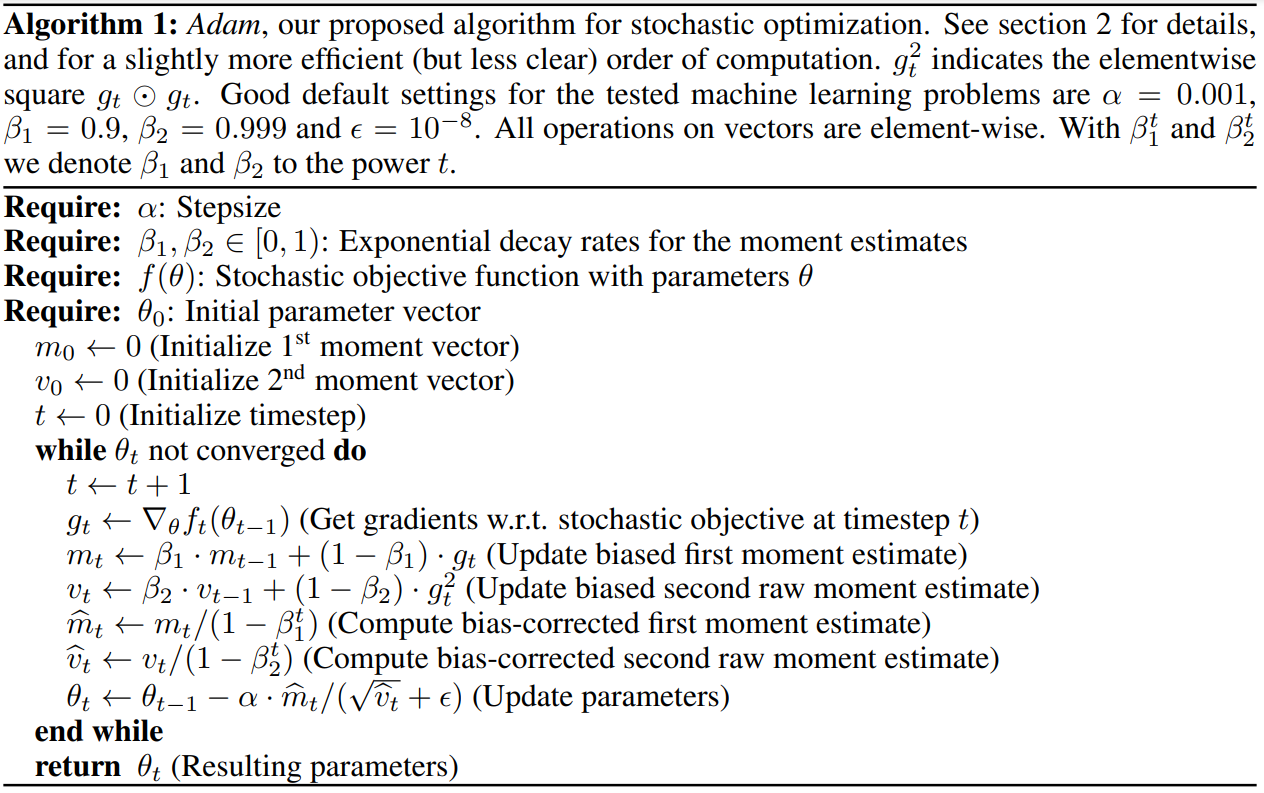
\includegraphics[width=0.8\textwidth]{pics/adam.png}
	\caption{Adam 计算过程}
	\label{fig:adam}
\end{figure}

可以看到计算完 $m_t, v_t$ 后又分别除以了 $1-\beta^t$, 随着 $t$ 的增大 $1 - \beta^t$ 逐渐接近 1. 为什么要这样呢? \textcolor{red}{由于 $m, v$ 的初始值都是 0, 在后续的估计中, $m, v$ 都会偏向于 0, 即 $m_t, v_t$ 不是 $E[g_t], E[g_t^2]$ 的无偏估计, 因此需要各自除以 $1 - \beta^t$, 具体的推到可以参考\href{https://arxiv.org/pdf/1412.6980.pdf}{论文}}.

网上找到一张梯度的一阶估计随时间步的变化(即 Fig.\ref{fig:adam} 中的 $m_t$), 如 Fig.\ref{fig:adam-gradient} 所示. 可以看到, 前面时间步的梯度在衰减. 
\begin{figure}[h]
	\centering
	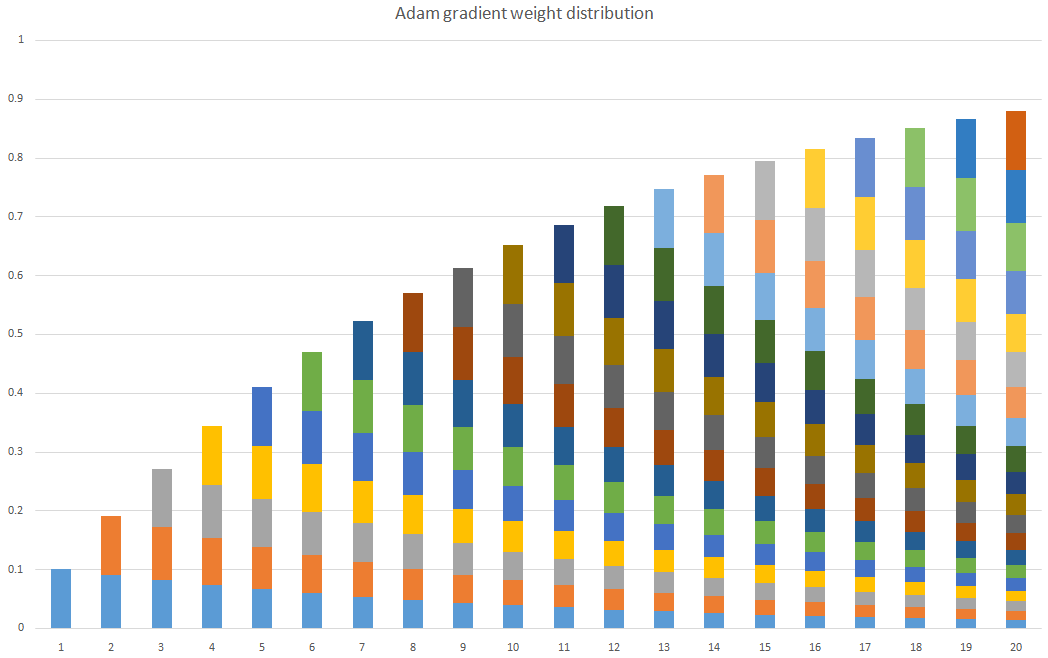
\includegraphics[width=0.85\textwidth]{pics/adam-gradient-weight-distribution.png}
	\caption{Adam 梯度一阶估计随时间步的变化(\href{https://www.jianshu.com/p/aebcaf8af76e}{来源})}
	\label{fig:adam-gradient}
\end{figure}

Adam 的特点: 1) 参数更新的步长与梯度的大小无关; 2) 对目标函数没有平稳要求; 3) 适用于大多非凸优化问题, 适用于大数据集和高维空间; 4) 由于 $m_t, v_t$ 可以看作是对固定时间窗口内梯度的估计, 因此可能出现梯度突变的情况, 导致后期学习率震荡, 导致模型无法收敛 (因为学习率不能收敛为 0). 

参考资料: 
\begin{itemize}
	\item \href{https://mp.weixin.qq.com/s/L9jCK5rtyq3fJZEBpLvagg}{从SGD到NadaMax, 十种优化算法原理及实现};
	
	\item 一篇讨论各种优化算法的论文:  \href{https://arxiv.org/pdf/1612.04010.pdf}{An empirical analysis of the optimization of deep network loss surfaces};
\end{itemize}

\subsection{常见损失函数及其特点}
\subsubsection{MSE}
MSE(mean squared error, 均方误差), 常用于回归任务中. 其形式较为简单: 
$$
l(y, \hat{y}) = (y - \hat{y})^2
$$
其中 $y, \hat{y}$ 分别为样本的真实值与预测值. MSE 的特点: 
\begin{itemize}
	\item 当 $|y - \hat{y}|$ 大于 1 时, MSE 会放大误差, 所以 MSE 容易受到异常点的影响;
	
	\item MSE 的梯度与误差的大小成正比;
\end{itemize}

\subsubsection{交叉熵损失函数}
常用于分类任务中. 最常见的莫过于而分类中的交叉熵损失函数了: 
$$
l(y, \hat{y}) = -(y \log \hat{y} + (1-y) \log (1-\hat{y}))
$$
其中 $y \in \{0, 1\}, \hat{y} \in (0, 1)$, $\hat y$ 表示样本为正样本的概率. 交叉熵更一般的形式为: 
$$
l(\boldsymbol{y}, \hat{\boldsymbol{y}}) = - \sum_{c=1}^K \boldsymbol{y}_c \log \hat{\boldsymbol{y}}_c
$$
其中 $\boldsymbol{y} \in \{0,1\}^K$ 表示样本所属的类别的 one-hot 编码, $\hat{\boldsymbol{y}}$ 是样本属于每个类别的概率(已归一化). 由于 $\boldsymbol{y}$ 是 one-hot 编码, 若样本的真实类别是 $c$, 则上式可简化为: 
$$
l(\boldsymbol{y}, \hat{\boldsymbol{y}}) = - \log \hat{\boldsymbol{y}}_c
$$
如果赋予了每个类别一个权重, 那么交叉熵损失可写为: 
$$
l(\boldsymbol{y}, \hat{\boldsymbol{y}}) = - \boldsymbol{w}_c\log \hat{\boldsymbol{y}}_c
$$
$\boldsymbol{w}_c$ 表示类别 $c$ 的权重. 

交叉熵损失的特点: 
\begin{itemize}
	\item 最后一层的权重更新时, 梯度与激活函数的导数无关, 不会因为输入落在饱和区而影响梯度的更新, MSE 则存在这个问题;
	
	\item 从交叉熵的式子中也可以看到, 计算损失时只利用到了在正确类别上的信息, 而其他类别的信息直接丢弃了. 这样可能会导致其他错误类别上的概率基本时一样的, 而忽略了其他类别之间的差异. 例如猫、虎、汽车的三个类别, 如果真实类别是猫, 那么直观上来看虎的概率还是应该大于汽车的概率的, 但交叉熵是将这些类别等同看待的, 忽略了类别见的差异和相关性;	
\end{itemize}

\subsubsection{Focal Loss}
Focal Loss(后续简称为 FL)为解决样本不平衡的问题, 更准确地讲, 是为解决难分类样本 (Hard Example) 和易分类样本 (Easy Example) 的不平衡问题. 对于样本不平衡, 其实通过上面的带权重的交叉熵损失便可以一定程度上解决这个问题, 但是在实际问题中, 以权重来解决样本不平衡问题的效果不够理想. 为什么呢?表面上是因为样本不平衡, 但实质上导致效果不好的原因也许并不是简单地因为样本不平衡, 而是因为样本中存在一些 Hard Example, 同时存在许多 Easy Example, Easy Example 虽然容易被分类器分辨, 损失较小, 但是由于其数量大, 它们累积起来依然于大于 Hard Example 的损失值, 因此我们需要给 Hard Example 较大的权重, 给 Easy Example 较小的权重. FL 是基于交叉熵损失的, 其定义为: 
$$
FL(\boldsymbol{y}, \hat{\boldsymbol{y}}) = -(1-\hat{\boldsymbol{y}}_c) \log \hat{\boldsymbol{y}}_c
$$
可以看到, 与交叉熵相比, FL 多了一个 $(1-\hat{\boldsymbol{y}}_c)$, 显然, 当模型对该样本分类的置信度越高, 则样本的损失越小(相比交叉熵更小), $(1-\hat{\boldsymbol{y}}_c)$ 可以起到样本权重的作用, 该值越小说明样本越容易被分类, 即为 Easy Example. 为了更好控制该权重, 改写 FL 为: 
$$
FL(\boldsymbol{y}, \hat{\boldsymbol{y}}) = -(1-\hat{\boldsymbol{y}}_c)^\gamma \log \hat{\boldsymbol{y}}_c
$$
其中 $\gamma$ 为超参数, $\gamma=0$ 则为交叉熵损失, 一般取 2, $\gamma$ 越大 Easy Example 带来的损失就越小, 对 Easy Example 起到的抑制就越大. 如果再要处理样本不均衡的问题, 可以再加上类别权重, 则 FL 改写为: 
$$
FL(\boldsymbol{y}, \hat{\boldsymbol{y}}) = - \alpha_c (1-\hat{\boldsymbol{y}}_c)^\gamma \log \hat{\boldsymbol{y}}_c
$$
其中 $\alpha_c$ 为类别 $c$ 的权重. 

\subsubsection{Sampled Softmax}

\subsubsection{Contrastive loss, Triplet loss} 
都是一种损失函数. 

Triplet loss用于训练差异较小的数据, 常用于人脸识别中. 以这种函数为损失函数时, 输入的一个样本是一个三元组(anchor, positive, negative), anchor是随机选择的一个样本, 而positive和negative分别于anchor为同类/异类数据. 在学习时, Triplet loss的目的就是让anchor的表征与positive的表征尽量靠近, 与negative的表征尽量疏远. 那么对于一个样本来说, Triplet loss写成公式:  
$$
\mathcal{L} = max( ||f(a)-f(p)||_2^2 - ||f(a) - f(n)||_2^2 + \alpha )
$$
公式的含义也很明显, 尽量使类内数据相近, 类间数据相离. 

Contrastive loss是对比损失, 也叫zero-one损失, 主要用来处理孪生网络中的paired data的关系. 通常Contrastive loss的输入是两个样本, 且各自都有一个标签, Contrastive loss的目标就是: 如果两个样本同类, 则loss更小, 否则loss更大. 写成公式: 
$$
\mathcal{L} = d_{ij}^2 \cdot Y_{ij} + (1 - Y_{ij} )max(margin - d_{ij}, 0)^2
$$
其中, $d_{ij}$就表示样本i, j之间的距离, 这个可以有多种形式的定义, $Y_{ij}$表示样本i, j的标签是否相同, margin是一个阈值, 如果$d_{ij}$超过阈值则应该尽量把它们划分开. 

\subsection{常见激活函数及其特点}
\subsubsection{sigmoid}
\begin{center}
	\begin{tikzpicture}
		\begin{axis}[
			legend pos=outer north east,
			xlabel = $x$,
			ylabel = {$f(x)$},
			]
			\addplot[color=red] {1/(1+exp(-x))};
			\addlegendentry{$f(x) = \frac{1}{1+e^{-x}}$}
		\end{axis}
	\end{tikzpicture}
\end{center}
这个恐怕是无人不知无人不晓了吧, 通常用于将神经元得输出转化成一个概率值. 

优点: 梯度平滑、易求导. 缺点: 
\begin{itemize}
	\item 计算复杂, 在正向和反向传播过程中都涉及到幂运算和处罚;
	
	\item 当输入值处在平缓区域时(即较大或较小), 导数接近于零, 可能会导致梯度很小/为零, 不利于更新参数;
	
	\item sigmoid 的输出不是零中心的;
\end{itemize}

\textbf{怎么解决 sigmoid 的梯度饱和的问题呢?} 1) 在 sigmod 之前引入 BN 层. 通过 BN 层对输入数据的分布进行规范化, 使其能够落在 sigmoid 的梯度较大的区域. 2) 替换激活函数. 建议非输出层的激活函数选用 ReLU; 3) 在模型重加入残差模块; 4) 采用 pre-training+fine-tuning 的方式训练模型, 即一层一层地训练隐层, 最后再进行微调; 5) 增加门控机制, 类似于 LSTM 和 GRU 中的门控单元.

\subsubsection{ReLU}
Rectified Linear Unit, 整流线性单元, 这个算是与 sigmoid 齐名的激活函数了: 
$$
relu(x) = max(0, x)
$$
优点: 计算速度很快, 而且导数很稳定(在大于 0 的部分为 1), 不会因为导数很小使得连乘后梯度很小. 缺点: 因为当输入小于 0 时输出为 0 且梯度为 0, 这其实相当于抛弃了一部分信息, 而且由于导数为零, 可能某些参数不能得到很好地学习. 

显然, Focal Loss 能够针对 Hard/Easy 样本给出不同的权重. 

\subsubsection{Leaky ReLU}
可以看到在 ReLU 里, 当输入为 0 时输出直接为 0, 导数也为 0. Leaky ReLU 对输入小于 0 时进行了修改: 
$$
Leaky-ReLU(x) = max(0, x) + a \cdot min(0, x)
$$
可以看到, 当 $x$ 大于零 时, 输出还是 $x$, 当 $x$ 小于 0 时, 输出为 $a x$. 

优点: 计算速度快, 且当输入小于 0 时输出不为零, 导数不为 0. 缺点: 多了一个超参数 $a$. 

\subsubsection{PReLU}
Parametric ReLU, 即参数化的 ReLU. 其形式与 Leaky ReLU 很像, 但是其中的 $a$ 成了可训练的参数: 
$$
PReLU(x) = max(0, x) + a \cdot min(0, x)
$$
其中的 $a$ 不再是超参数, 而是可训练的了. 

\subsubsection{Dice}
\begin{figure}[h]
	\centering
	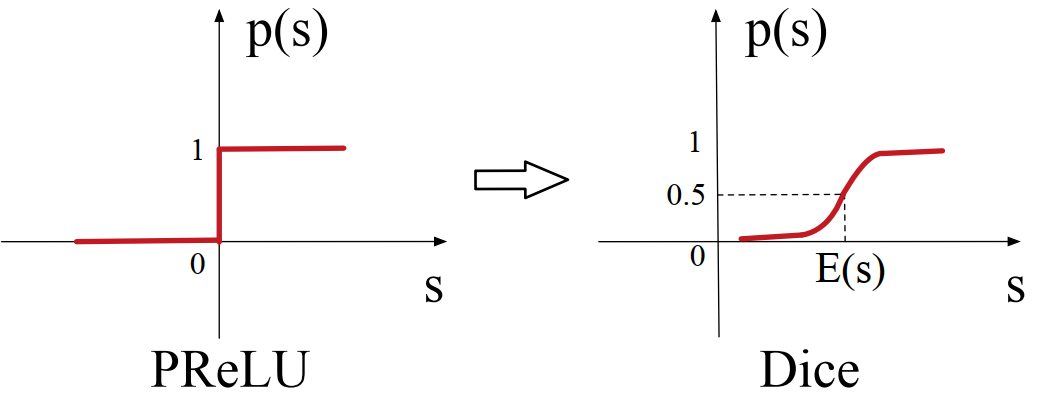
\includegraphics[width=.6\textwidth]{pics/prelu-dice.png}
	\caption{Rectified Point of PReLU and Dice}
	\label{fig:prelu_dice}
\end{figure}
Data Dependent Activation Function, Dice激活函数诞生于 DIN 中, 根据 PReLU 改造而来. ReLU 类函数的阶跃变化点在 x=0 处, 意味着面对不同的输入这个变化点是不变的, PReLU 和 Dice 的阶跃点比较如 Fig.\ref{fig:prelu_dice} 所示. DIN 中改进了这个变化点的位置, 让它根据数据的分布(神经元输出的均值和方差, 与 BN 类似)自适应来调整阶跃点的位置: 
$$
dice(x) = p(x) \cdot x + (1 - p(x)) \cdot \alpha \cdot x
$$
其中 $p(x) = sigmoid( BN(x))$, $BN(x) = \frac{x - E(x)}{\sqrt{Var(x) + \epsilon}}$. 与 PReLU 相比, 其实相当于将 max/min 这种硬的划分改成了软(即以概率 $p(x)$)的划分. 从公式和 Fig.\ref{fig:prelu_dice} 中可以看出, 均值控制了阶跃点的位置, 方差控制了阶跃处的变化速率, 即斜率. 

\subsubsection{Softplus}
Softplus 函数可以看作是 ReLU 函数的平滑, 即 $x^+ = max(0, x)$ 的平滑, 因此叫做 Softplus. 形式为: 
$$
Softplus(x) = log(1+e^x)
$$
显然, Softplus 输出的值域是 $(0, +\infty)$. 

\subsection{学习率调整策略}
\paragraph{WHY?}学习率 (Learning Rate, LR) 是基于梯度下降的优化算法中不可或缺的一部分, 目前的深度学习模型无一不使用梯度来优化模型参数, 设置学习率是不可避免的. 在训练过程中, 学习率是否应该变化, 应该如何变化对模型的收敛效果有很大的影响. 看看LR对学习过程的影响: 
\begin{myitemize}
	\item 学习率设置太小, 需要花费过多的时间来收敛
	\item 学习率设置较大, 在最小值附近震荡却无法收敛到最小值
	\item 进入局部极值点
	\item 停在鞍点处, 不能够在另一维度继续下降
\end{myitemize}

\paragraph{哪些策略}总体来说, LR可以是固定的, 即整个训练过程中不变; 也可以是动态的, 即在训练时变化, 当让根据不同的变化方式动态策略又有多种. 
\begin{myitemize}
	\item 固定LR, 整个训练过程中LR保持不变. 固定LR适用于优化目标为凸函数的情况, 当为非凸时可能会收敛到局部极值点然后开始振荡. 且LR的大小选择很重要, 为了保证收敛一般会设置的比较小. 
	\item LR衰减 (LR Decay) , 即LR随着训练进程而减小. 在训练初期大步长向目标前进, 后期小碎步靠近最优点. 常见的衰减策略: 
	\begin{myitemize}
		\item 固定步长衰减, 即每隔一定步数/epoch数, 就对LR衰减一次
		\item 指数形式衰减, 即以指数形式衰减, 通常是$LR = LR \times \gamma^{n}$, 其中$\gamma$由用户指定, $n$可以是\textit{step}或\textit{epoch}
		\item 多步长衰减, 即在不同的区间使用不同的LR. 通常是设置一系列的epoch锚点, 达到锚点后LR就衰减一次, 因此也要设置$\gamma$
	\end{myitemize}
	\item 基于Armijo准则步长搜索算法, 遵循两个准则搜索步长: 1) 目标函数值下降幅度要大于一定阈值; 2) 搜索的步长不应该太小. 这种步长调整策略较为耗时
	\item 循环学习率, 即LR的变化呈现周期性, 当然也可以每过一个周期LR就衰减一次
	\item 自适应学习率, 即自定义一些规则来决定学习率的如何改变
	\item 不同的网络层使用不同的LR
\end{myitemize}
以上这些LR调整策略只是简单介绍了调整策略的思想, 在实践中, 深度学习框架一般会提供一些LR调整策略的接口, 也可以自定义调整策略. 

参考资料: \href{https://lumingdong.cn/setting-strategy-of-gradient-descent-learning-rate.html}{梯度下降学习率的设定策略}. 

\section{经典}
\subsection{Residual learning block}
跳跃连接,基本的残差块如Fig.\ref{fig:residual}所示(当然残差块不止有这一种形式,可以根据需求定义不同的残差块)。残差学习由何凯明基于以下问题提出:给定一个学习问题后,逐渐加深网络的层的时候,模型的效果应该是逐渐提升的或者不能低于原来模型的效果,但是在实验中发现通常加深后模型的效果反而变差了。按理来说就算不能提升了,额外增加的层也可以学习到一个恒等映射来保持效果不变啊,但是为什么反而下降了呢?这便是\textbf{模型退化问题}。

假设原本要学习的问题是$\mathcal{H}(x)$,之前的想法是直接学习它,在残差学习中,将它进行分解$\mathcal{H}(x) = \mathcal{F}(x) + x$,由于$x$是已知的,那么只需要学习$\mathcal{F}$就好了,$\mathcal{F}$也就是所说的残差。

\textbf{为什么这样会有效呢?}由于神经网络中通常都会使用非线性函数来拟合复杂的函数,但是对于线性关系却有点力不从心(可能这就是为什么不能学习到恒等映射的原因吧)。残差学习不仅保留了学习非线性函数的能力,也提高了线性函数的学习能力 --- $\mathcal{F}$为0即可。Resudial Learning的这种能力使得更深的网络称为可能。

\begin{figure}[h]
	\centering
	\includegraphics[width=.4\textwidth]{pics/Residual.png}
	\caption{Residual}
	\label{fig:residual}
\end{figure}

\subsection{Dense Connection}
稠密连接,如Fig.\ref{fig:dense block}所示。每一层与之前的所有层都有连结。用$H_l$表示第$l$层,$\boldsymbol{X}_l$表示第$l$层的输出,则$\boldsymbol{X}_l = H_l(\boldsymbol{X}_0, \boldsymbol{X}_1, ..., \boldsymbol{X}_{l-1})$。

有以下优点:1)减轻了梯度消失问题;2)加强了特征的传播,能够有效的利用学习到的特征;3)能够利用多层次的特征。
\begin{figure}[h]
	\centering
	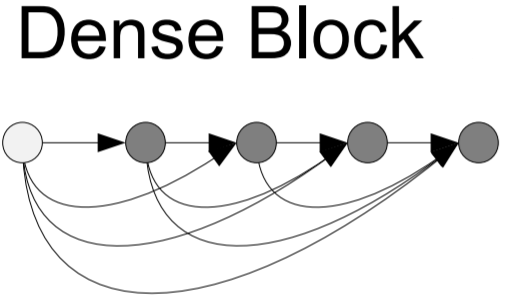
\includegraphics[width=.4\textwidth]{pics/dense block.png}
	\caption{Dense Block}
	\label{fig:dense block}
\end{figure}

\subsection{Dilated Convolution}空洞卷积。在pooling时,可以减小feature map的尺寸,也能增大每个元素的感受野但是也损失了空间信息。在进行分割时,pooling损失的那部分信息是难以复原的。dilated卷积是一种特殊的卷积,与通常的卷积不同,dilated卷积会在\textbf{卷积核元素之间插入空格},其实相当于一个更大的卷积核,而那些插入的卷积核的值一直为0。如Fig.\ref{fig:dilation}所示。Dilation卷积可以在不做pooling损失信息的情况下增大感受野,pooling虽然可以增大感受野但是失去了位置信息,难以从pooling后的层恢复到原来的信息,而dilation卷积不仅增大了感受野,还保留了特征图中元素的相对空间信息。
\begin{figure}[h]
	\centering
	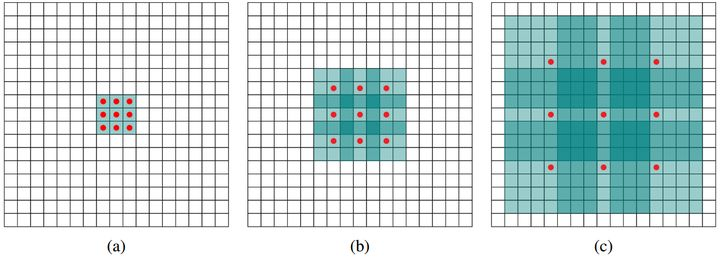
\includegraphics[width=.8\textwidth]{pics/dilation.jpg}
	\caption{Dilation Convolution}
	\label{fig:dilation}
\end{figure}

\subsection{1 $\times$ 1 Conv}
$1\times 1$卷积很显然,就是卷积核的长宽均为1,用$c_i$ 和$c_o$  分别表示输入和输出通道的数目,为了获得多个通道的输出,可以为每个输出通道创建一个形状为$c_i\times 1 \times 1$ 的卷积核张量,这样卷积核的形状是$c_o \times c_i \times 1 \times 1$。

由于$1\times 1$卷积的长宽为1,无法关注到周围像素的信息,只能关注到同一位置不同通道上的信息,其作用主要由以下几点:
\begin{itemize}
	\item 融合多个通道间的信息
	\item 在不改变feature map尺寸的情况下改变feature map的通道数,例如在图像分割中
	\item 降低参数量
	\item 在以每像素为基础应用时,$1\times 1$卷积相当于全连接层
\end{itemize}
更多解释可参考动手学深度学习:\href{https://zh-v2.d2l.ai/chapter_convolutional-neural-networks/channels.html#times-1}{$1\times 1$  卷积层}

\subsection{LSTM}

\subsection{GRU}


\clearpage
\part{Graphs}
{\noindent}	 \rule[-10pt]{17.5cm}{0.5em}\\
\section{Graphs}
% 记录一些常见的图的概念
\subsubsection{图基本概念}
\paragraph{Motif} 形式上是一个连通子图,强调这个Motif的拓扑结构。Motif可能是某种经常出现在图中的结构,可以认为时一种反复出现的结构模式。相同结点数的motif可能会有多种结构。

\paragraph{Weisfeiler-Lehman isomorphism test}  图同构测试。对于两个图$G_1, G_2$,WL test能够判断它们是否同构,但是也存在一些特殊的例子,WL test会将非同构的两个图判定为同构的。算法过程如下:
\begin{enumerate}
	\item 对$G_1, G_2$中的结点都赋予一个标签,都为1;
	\item 对于每个结点$v$重复执行:
	\begin{enumerate}
		\item 汇集$v$的邻居结点的标签,放在一个列表里,$S_v = \{u_l | u \in \mathcal{N}_v \}$
		\item 将$v$的标签$v_l$和S组合成一个pair---$(v_l, S_v)$
	\end{enumerate}
	\item 利用一个hash函数将每个结点的$(v_l, S_v)$映射成一个新的标签,将新的标签赋予给对应的结点。至此一轮迭代就结束了,如果图中结点的标签都没发生变化则结束,否则返回步骤2.
\end{enumerate}
上述过程是针对一个图来说的,可以同时分别对$G_1, G_2$执行上述算法。
当迭代结束后怎么判定两个图是否同构呢?
WL test中是这样做的:\\
分别计算图中每个标签的数量(也就是标签的分布),可能会得到类似这样的一个结果(1: 2, 2:3, ...),这表示标签1出现了2次,标签2出现了3次。如果最后两个图这个结果是一致的,那么不排除它们同构的可能性。

基于WL test 算法,WL subtree kernel\cite{shervashidze2011weisfeiler} 构建以某个结点为根的子树,来代表该结点的特征。

\paragraph{图算法(GNN)中常用的benchmar以及数据集} 常用的图数据集主要可以分为这几类:
\begin{itemize}
	\item 生物信息类的图数据。如MUTAG, PTC, NCI1,PROTEINS 分子,药物的一些图数据
	\item 社交网络。如Facebook, Reddit 等
	\item 引文网络。如 Cora, PubMed, Citeseer等
\end{itemize}

斯坦福大学的SNAP组有很丰富的图网络数据集:\href{http://snap.stanford.edu/data/index.html}{Stanford Large Network Dataset Collection}


\paragraph{Heterogeneous graph, Attributed graph}同构图和属性图,同构图中,有多种类型的结点和边。Attributed graph中结点会有较丰富的属性(个人感觉可以理解为特征)。一个简单的分类:
\begin{table}[h]
	\centering
	\begin{tabular}{|c|c|c|c|}
		\hline
		\rowcolor[HTML]{4371C3} 
		{\color[HTML]{FFFFFF} \textbf{Graph Types}}                            & {\color[HTML]{FFFFFF} \textbf{Homogeneous}} & {\color[HTML]{FFFFFF} \textbf{Multi-Relational}} & {\color[HTML]{FFFFFF} \textbf{Heterogeneous}} \\ \hline
		\rowcolor[HTML]{CED6EA} 
		\textbf{\#of node types}                                               & \textbf{1}                                  & \textbf{1}                                       & \textbf{\textgreater{}1}                      \\ \hline
		\rowcolor[HTML]{E9EBF6} 
		\multicolumn{1}{|l|}{\cellcolor[HTML]{E9EBF6}\textbf{\#of edge types}} & \textbf{1}                                  & \textbf{\textgreater{}1}                         & \textbf{\textgreater{}=1}                     \\ \hline
	\end{tabular}
\end{table}

\paragraph{Graph Kernel}

\paragraph{Dynamic graph, Streaming graph}动态图和流图。动态图主要指在给定的(static)的结点集上,随着时间,边发生变化;而流图则是结点集和边都会随着时间而变化。

除了结点和边的变化,可能结点/边的标签也会发生变化,更具体的,结点/边的属性也会变化。

\paragraph{图的同构}对于两个图$\mathcal{G}_1 = (V_1, G_2), \mathcal{G}_2=(V_2, E_2)$,如果两图之间的结点能够一一对应,令该映射为$f$,

若$\forall v_i^1, v_j^1 \in V_1, v_i^2, v_j^2 \in V_2$,$f(v_i^1) = v_i^2, f(v_j^1) = v_i^2$,当$(v_i^1, v_j^1) \in E_1$有$( f(v_i^2), f(v_j^2) ) \in E_2$,则称$\mathcal{G}_1, \mathcal{G}_2$是同构的,存在同构映射$f$。

\subsubsection{结点邻居采样}
在图机器学习中,生成结点表征可以说是最基本的事儿了。不管是随机游走、矩阵分解还是图神经网络的方式,最终都会得到结点的表征。其中不可绕过的一个就是结点的邻居。
在随机游走中,会类似于语言模型中词语的上下文环境一样为结点构造上下文,每个结点产生的随机游走路径就是一个上下文。游走的过程可以看作是对结点邻居进行采样的过程。矩阵分解中,通常是构造图的Laplacian矩阵,再进行分解,用特征向量来表示结点表征,对这个不是很了解,就不多说了。到了图神经网络中,节点邻居更是成了主角。从GCN原论文\cite{kipf2017semi-supervised} ==> GraphSage\cite{hamilton2017inductive} ==> FastGCN\cite{chen2018fastgcn} ==> VR-GCN\cite{chen2018stochastic} ==> ... 。GCN中结点的邻居采样方式五花八门。

\begin{enumerate}
	\item GCN原论文中,再进行图卷积时需要把整个graph全部加载进内存,为了求一个结点的表征需要对整个graph进行卷积
	\item GraphSage中,并不使用结点的所有邻居,而是对每个结点的邻居进行采样,得到固定数目的采样后的邻居
	\item FastGCN中引入了importance sampling
	\item 审稿时发现的根据attention distribution 和 uniform distribution的KL散度选top-k的采样。这种方法可以发现比较重要的结点,而不是均匀地参与到其邻居的结点
\end{enumerate}

\subsubsection{DeepWalk \& Node2Vec}
二者都是学习结点表征的方法,都是通过游走的方式来生成一个节点的context,在通过SkipGram的方式来学习结点表征。二者关键的差别就在生成context的方式,即游走方式上。

\begin{itemize}
	\item DeepWalk不适用于有权图,不能学习权重对graph、结点带来的影响;Node2Vec能够处理带权图
	\item DeepWalk中使用的是RandomWalk。给定一个结点$v$,下一步访问的结点通过均匀采样$v$的邻居结点来得到
	\item Node2Vec中用了两个参数来控制游走,即如何采样下一个结点
\end{itemize}
重点介绍以下Node2Vec中的randomwalk,如Fig.\ref{fig:node2vec}所示。
\begin{figure}[h]
	\centering
	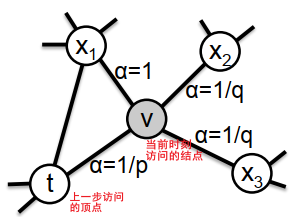
\includegraphics[width=.5\textwidth]{pics/node2vec.png}
	\label{fig:node2vec}
	\caption{Node2Vec中的随机游走}
\end{figure}
Node2vec中的随机游走是二阶的随机游走,为什么叫二阶的呢?在Deepwalk中,随机游走只与当前时刻访问的结点有关,直接从当前节点的邻居中进行均匀采样,这叫一阶。Node2vec中的二阶是指:当前访问的结点$v$,下一步访问的某个节点概率将由上一时刻访问的结点$t$和$v$与邻居的边的权重决定,这是一个二阶马尔科夫链。
$$
P(c_{i}=x \mid c_{i-1}=v)=\left\{\begin{array}{ll}
	\frac{\pi_{v x}}{Z} & \text { if }(v, x) \in E \\
	0 & \text { otherwise }
\end{array}\right.
$$
其中$P(c_{i}=x \mid c_{i-1}=v)$表示当前时刻访问$v$,下一时刻访问$x$的概率,$Z$用于归一化,$\pi_{vx} = \alpha_{pq}(t,x) \cdot w_{vx}$,$\alpha_{pq}(t, x)$为:
$$
\alpha_{p q}(t, x)=\left\{\begin{array}{ll}
	\frac{1}{p} & \text { if } d_{t x}=0 \\
	1 & \text { if } d_{t x}=1 \\
	\frac{1}{q} & \text { if } d_{t x}=2
\end{array}\right.
$$
可见$\alpha_{pq}(t, x)$是一个由$p, q$参数化的函数,函数的自由变量是$t, x$即上一时刻访问的结点和下一时刻访问的结点,其中$d_{tx} \in \{0, 1, 2\}$表示$t, x$间的最短距离。

$p, q$就是控制游走的两个参数:
\begin{itemize}
	\item Return Parameter,$p$,该参数控制下一时刻访问$t$的可能性,如Fig.\ref{fig:node2vec}所示,$p$越小,越有可能访问上一时刻已经访问过的结点$t$,当然还要考虑$w_{vt}$
	\item In-Out Parameter,$q$,该参数能够控制是BFS还是DFS。当$q>1$时,在$p$不变的情况下,访问$d_{tx} = 1$的结点的概率会增大,这就是BFS,当$q<1$时,则会增大访问$d_{tx} = 2$的结点的概率会增大,这就是DFS
\end{itemize}
\begin{figure}[h]
	\centering
	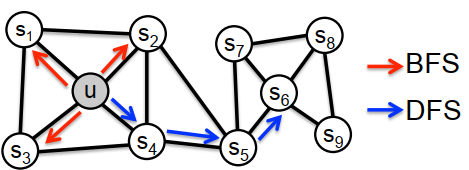
\includegraphics[width=.8\textwidth]{pics/node2vec2.png}
	\label{fig:node2vec2}
	\caption{Homophily与Structure Equivalence}
\end{figure}

论文中将这叫做Biased random walk,通过调整游走的参数$p,q$能够使学习到的表征在同质性(Homophily)和结构相似性(Structure Equivalence)间平衡。BFS能够探索探索homophily,即距离相近的结点,如Fig.\ref{fig:node2vec2}所示,$s_1, s_2, s_3, s_4$是与$u$相邻的结点,它们的表征应该相似;DFS使得探索到更远的地方,能够发现与$u$结构类似地结点,如$s_6$,它俩地表征也应该相似。所以学习到的表征既能体现结点地同质性,也能体现结点地结构相似性。

\section{Knowledge Graph}
\subsubsection{KG中的文本信息抽取}
从纯文本数据中获取有价值的数据,组织成结构化的形式或半结构化的形式。主要包含这几个过程:实体识别、实体消歧、关系抽取及事件抽取。
\paragraph{实体识别}从文本中识别出实体信息。

\paragraph{实体消歧}消除指定实体的歧义。可以分为两类:
\begin{itemize}
	\item 实体链接:将给定文本中的实体指称项链接到已有知识图谱中的某个实体上
	\item 实体聚类:假设已有知识图谱中并没有已经确定的实体,在一个给定一个语料库的基础上,通过聚类的方法消除语料中所有同一实体指称项的歧义,具有相同所指的实体指称项应被聚为一类
\end{itemize}

\paragraph{关系抽取}获取两个实体之间的语义关系。

\paragraph{事件抽取}从描述事件信息的文本中抽取出用户感兴趣的事件信息并以结构化的
形式呈现。
\tbc{red}{kg中的事件能否看作一个subgraph?}



\clearpage
\part{Natrual Language Process}
{\noindent}	 \rule[-10pt]{17.5cm}{0.5em}\\
\section{基础}
\subsection{常见NLP任务}

\subsubsection{命名实体识别}
NLP中的命名实体识别(Named Entity Recognition)指的是将识别出文本中描述实体的词汇,比如人名、地名、组织机构名、股票基金、医学术语等,更一般地讲,不同的领域会有不同的实体,用于描述该领域内的实体对象。NER的目的就是识别出文本中实体与其他文本的边界和实体的类别。主要以下几个难点:
\begin{itemize}
	\item 实体的数量是无穷的。不同的领域会有不同的实体,且实体并不是定量的,会不断的增加
	\item 实体的构词灵活。同一个实体可能会有多个名字,比如实体的简写;实体也可能是嵌套形成的
	\item 类别模糊。同一个实体在不同的语境下可能会有不同的类别
\end{itemize}

命名实体的识别,从某个角度来看可以视作一个序列标注问题。具体做法是将命名实体附着到{B, M, E, S}标签。其实,词性标注问题也可以以这样的方法来处理。更一般地看,词性标注与命名实体识别是同一个问题,它们都需要对文本进行分词,词性标注中的词性和NER中的实体类别是等价地。

\subsubsection{语法分析}
分析句子中的语法结构并将其表示为容易理解的结构(通常为树形结构)。
\paragraph{短语结构树}根据上下文无关文法将句子/短语分解为树状结构。短语结构语法(上下文无关文法)描述了如何自定向下地生成一个句子,同样句子/短语也可以通过短语结构语法进行分解。这其实和编译原理中的上下文无关文法是很类似的,也是通过很多产生式进行推导,那么是否可以使用编译原理中的词法分析来解决这个问题呢?

\paragraph{依存句法树}关注的是句子中词语之间的语法关联系,并将其约束为树形结构。在句子中,如果一个词语修饰另一个词语,则称修饰词为从属词,被修饰词为支配词,两者之间的语法关系称为依存关系,在可视化时,由支配词指向从属词。依存句法树描述了句子中的各个词之间的依赖关系,一般约定同一个词不能依存于多个词。

\textbf{复合性原理}:一个复杂表达式的意义是由其各组成部分的意义以及结合它们的规则决定的。通过将句子分解为短语、分解短语为单词,下游应用会得到更多更深层次的结构化信息。

\subsubsection{序列标注}
通常也可以看作是token级别的分类问题:对每一个token进行分类。token级别的分类任务通常指的是为为文本中的每一个token预测一个标签结果,如命名实体识、词性标注等。
\begin{itemize}
	\item NER (Named-entity recognition 名词-实体识别) 分辨出文本中的名词和实体 (person人名, organization组织机构名, location地点名...).
	\item POS (Part-of-speech tagging词性标注) 根据语法对token进行词性标注 (noun名词, verb动词, adjective形容词...)
	\item Chunk (Chunking短语组块) 将同一个短语的tokens组块放在一起。
\end{itemize}

\subsubsection{问答系统}
问答式信息检索是一种允许用户以自然语言方式询问,系统从单语或多语文档集中查找并返回确切答案或者蕴含答案文本片断的新型信息检索的方式。问答系统分类如Fig.\ref{fig:qa}所示。
\begin{figure}[h]
	\centering
	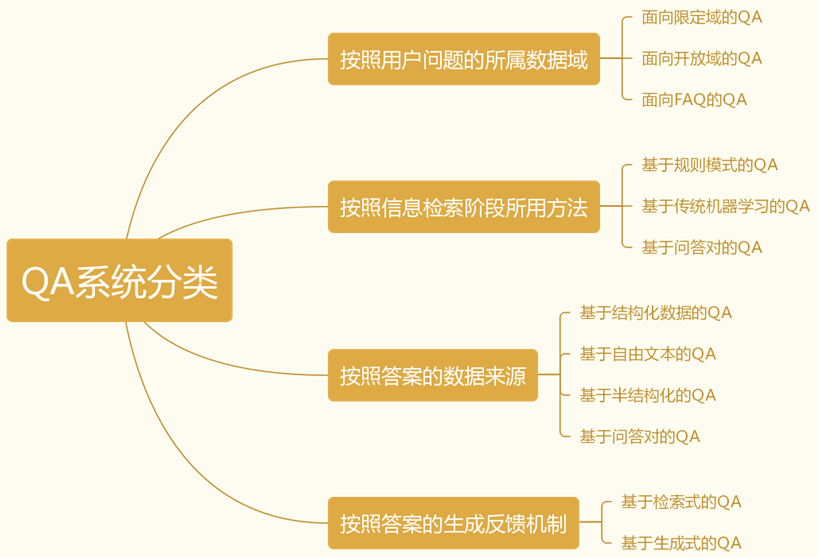
\includegraphics[width=.7\textwidth]{pics/qa.png}
	\caption{问答系统分类,源图\href{https://blog.csdn.net/sinat_33231573/article/details/83473741}{出处}}
	\label{fig:qa}
\end{figure}









\subsection{预训练}
预训练在很多领域上都有应用,如CV、NLP。当用深度学习来解决一个任务时,使用的深度模型通常会包含很多参数,我们需要使用大量的数据来更新我们的参数使之能够在特定的任务上取得不错的效果。一般,我们会对模型的参数初始化,然后使用大量带标签的数据来更新模型参数。

但实际情况是,带标签的数据总是很少的。

\begin{figure}[h]
	\centering
	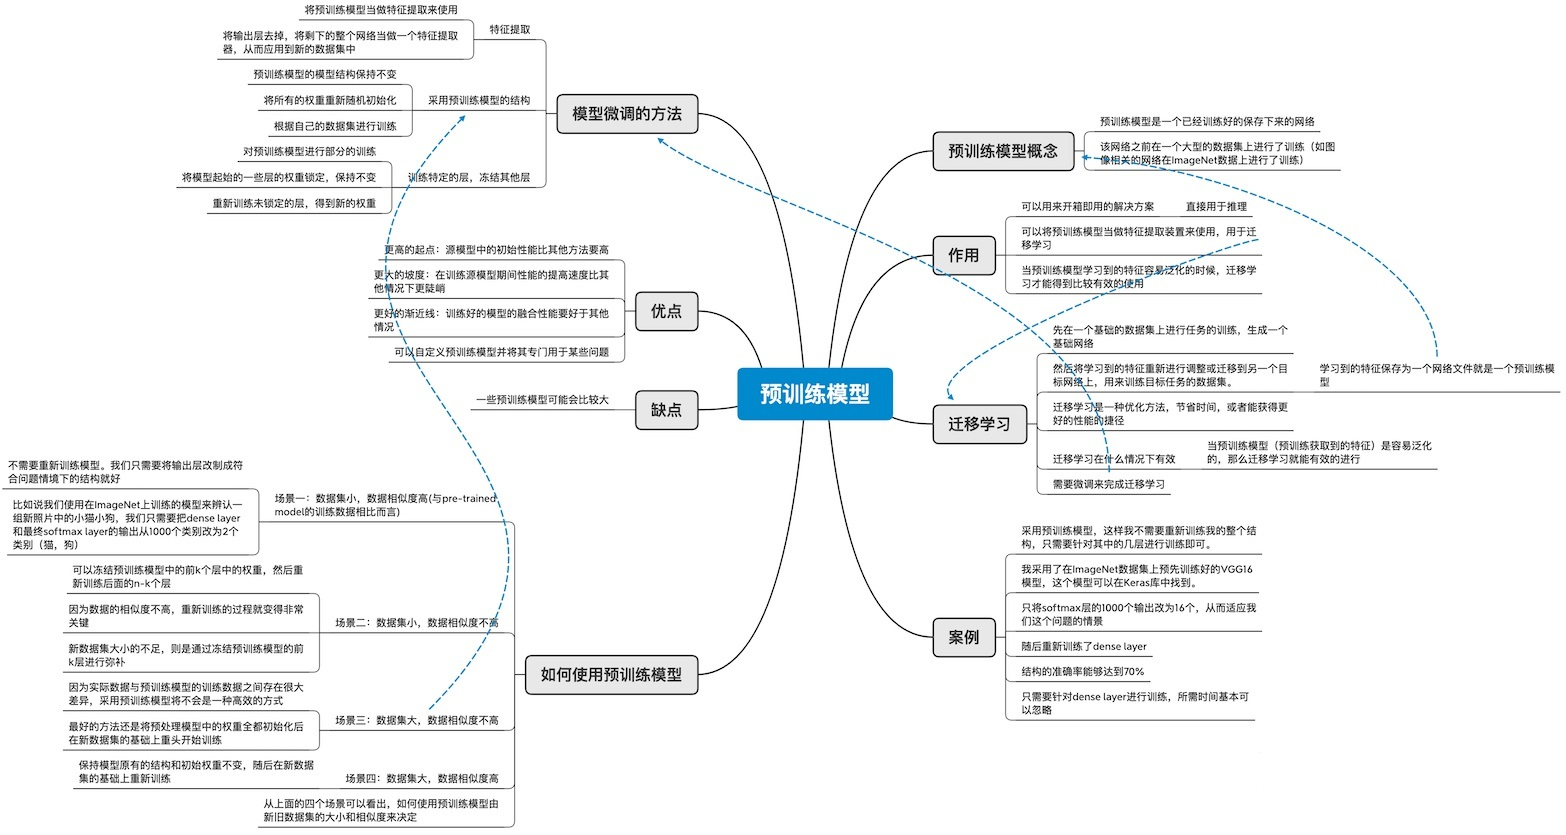
\includegraphics[width=\textwidth]{pics/pre-train.jpg}
	\caption{预训练模型(\href{https://www.zhihu.com/question/327642286/answer/1215812016}{出处})}
	\label{fig:pre-train}
\end{figure}
预训练通常在大量无监督的数据上学习(可以是无监督的学习任务、简单的有监督学习任务),用无监督的数据帮助模型的参数收敛,后续再在监督数据上进行调整。






\section{经典算法}
\subsection{统计自然语言处理}



\subsubsection{概率图模型}
将联合概率分布以图的形式来表示, 可以分为有向概率图模型和无向概率图模型. 
概率图模型中, 将随机变量表示为结点, 相关联的随机变量之间会有边连接. 

有向图模型中按变量的因果关系进行连接, 可以刻画变量之间的因果关系. 有向图表示的联合概率可以根据图中的变量依赖关系分解成多个条件概率的积. (听着有点像拓扑图)

无向图模型没有体现出因果关系, 强调的是变量之间的相互关系. 无向图模型将联合概率分布分解为“无向图中-最大团上-随机变量的函数-的乘积”. 





\subsubsection{词袋模型}
用于表示文档/句子(其实句子可以看作只有一个句子的文档)的一种方法. 
词袋模型一般会先构建一个词表, 每个文档经过分词后, 可以使用不同的统计量来构建文档/句子的向量, 词表之外的词不予考虑. 可以选用的不同的统计量有: 
\begin{itemize}
	\item 词频
	\item 布尔词频
	\item TF-IDF
	\item 词向量
\end{itemize}

\subsection{使用朴素贝叶斯分类器进行文本分类}
首先, 给定类别数为$c$, 每个文档的特征向量长度为$n$. 

朴素贝叶斯分类器是一个生成式的分类器, 其计算的是$p(Y | X)$, 对于生成模型, 重要的是要学习联合分布$p(X, Y)$, 朴素贝叶斯通过训练数据学习该联合分布: $p(X, Y) = p(Y)p(X|Y)$. 对于给定样本$X^i$, 对其进行分类可形式化为: 
$$
y = \mathop{argmax}_{c_k} p(Y=c_k | X=X^i) = \mathop{argmax}_{c_k} \frac{p(X=X^i | Y=c_k) p(Y=c_k)}{p(X=X^i)}
$$
朴素贝叶斯中假设样本的特征之间是相互独立的, 即$p(X)=p(X_1=x_1, ..., X_n=x_n) = p(X_1=x_1) ... p(X_n=x_n)$. 那么为了得到样本$X^i$的类别, 只需要计算出$p(X=X^i | Y=c_k),  p(Y=c_k), p(X=X^i)$即可. 而对于某一个样本的分类, $p(X^i)$对分类是没有帮助的, 在$Y$取不同类别时是不会变化的, 故可以不计算$p(X^i)$. 那么剩下的需要计算的只有出$p(X=X^i | Y=c_k),  p(Y=c_k)$了. 

$p(Y=c_k)$是很好计算的, 只需要统计训练数据中类别为$c_k$的样本所占的比例即可. 由于特征之间独立的假设, 所以$p(X^i | Y=c_k) = \prod_{j=1}^{n} p(X_{j}^{i}=x_j | Y=c_k)$. 这个概率也只需要从训练数据中统计即可, 统计每个类别下, 特征向量的第$j$维取$x_j$的比例即可. 

关于样本的特征向量: 通常可以采用词袋模型的方法来表示一个文本/句子. 

\subsection{马尔科夫链/隐马尔科夫链}
马尔可夫模型主要用于研究时间序列的分布的, 若已有一个是时间序列: $X_0, X_1, X_2, ..., X_n$, 马尔可夫模型要解决的就是这些随机变量的取值是如何随着时间而变化的、每个随机变量取值的概率 --- 这些随机变量取值的分布. 随机变量的取值可以称为状态. 那么问题就成了: 
$$
P(X_0=s_0, X_1=s_2, ..., X_n=s_m) = ?
$$
或者说, 下一个时刻的随机变量的取值问题: 
$$
P(X_n | X_0=s_0, X_1=s_2, ..., X_{n-1}=s_{m-1}) = ?
$$
为了简化这个问题, 有了马尔科夫假设. 

(1阶)马尔可夫假设: 当前状态的取值只取决于前一个时刻的状态. 即: 
$$
P(X_n | X_0=s_0, X_1=s_2, ..., X_{n-1}=s_{m-1}) = P(X_n | X_{n-1}=s_{m-1})
$$
满足这样性质的一系列随机变量串联在一起就是马尔科夫链了. 

那隐马尔科夫链与马尔科夫链又有什么关系呢?
隐马尔科夫模型描述的是两个时序序列的联合分布: $p( \boldsymbol{X}, \boldsymbol{Y} )$, 其中$\boldsymbol{X}, \boldsymbol{Y}$均为时序序列, 通常称$\boldsymbol{X}$为观测序列, $\boldsymbol{Y}$为状态序列 --- 不可观测序列. 其中观测序列/状态序列均可视为随机变量序列(注意, 同一时刻的观测变量和状态变量并不是独立的), 观测变量序列的取值为可观测值, 状态变量序列的取值为状态值 --- 与马尔可夫模型中的状态含义一致. 隐马尔科夫模型的假设: 
\begin{itemize}
	\item 当前状态变量$\boldsymbol{Y}_t$的取值仅以来与前一个状态变量$\boldsymbol{Y}_{t-1}$的取值有关, 连续多个状态变量的取值则构成隐马尔科夫链
	\item 任意时刻的观测变量$\boldsymbol{X}_t$取值仅依赖于该时刻的状态变量的取值$\boldsymbol{Y}_t$
\end{itemize}

一个隐马尔科夫模型可以表示为: $\lambda = (\boldsymbol{\pi}, \boldsymbol{A}, \boldsymbol{B})$, 含义如下: 
\begin{itemize}
	\item $\boldsymbol{\lambda}$: 初始状态概率向量, 即初始时刻的状态变量$\boldsymbol{Y}_0$取值为各个状态的概率
	\item $\boldsymbol{A}$: 状态转移概率矩阵, 即上一时刻的状态变量取某值时, 当前时刻状态变量取值的概率分布: $p(\boldsymbol{Y}_t=s_j | \boldsymbol{Y}_{t-1}=s_i)$
	\item $\boldsymbol{B}$: 发射概率矩阵, 即当前状态变量取某值时观测变量取某观测值的概率分布: $p(\boldsymbol{X}_t=o_j | \boldsymbol{Y}_t=s_j)$
\end{itemize}

其实, 可以看出马尔可夫模型是隐马尔科夫模型的一个特例 --- 状态变量序列与观测变量序列相同, 状态值即为观测值, 每个状态只对应一个观测值即本身. 

隐马尔可夫模型的三个应用: 
\begin{itemize}
	\item \textbf{样本生成问题}: 给定模型$\lambda = (\boldsymbol{\pi}, \boldsymbol{A}, \boldsymbol{B})$, 生成满足模型约束的样本 --- 观测序列即对应的状态序列
	\item \textbf{模型的训练}: 给定训练数据 --- 观测序列即对应的状态序列, 估计模型参数$\lambda = (\boldsymbol{\pi}, \boldsymbol{A}, \boldsymbol{B})$
	\item \textbf{序列预测}: 已知模型参数$\lambda = (\boldsymbol{\pi}, \boldsymbol{A}, \boldsymbol{B})$, 给定观测序列, 求状态序列
\end{itemize}

怎么解决上述的三个问题呢?

对于样本生成问题, 其实很简单, 指要逐步采样状态, 得到一个状态序列, 在根据每一步的状态取值采样得到观察值, 就可以得到观测序列, 样本生成就完成了. 

对于模型的训练问题, 需要估计的参数为: $(\boldsymbol{\pi}, \boldsymbol{A}, \boldsymbol{B})$, 对于$\boldsymbol{\lambda}$则统计所有的状态序列中, 计算以每个状态为开头的序列的频率即可, 其他两个概率矩阵的训练类比即可. 

对于序列预测问题可以通过维特比算法解决. 给定一个观测序列, 求解最有可能的状态序列. 本质上这是一个搜索问题, 搜索最有可能的状态序列, 使观测序列的似然概率最大. 简要地说一下. 

维特比算法通过动态规划的方法解决这个问题. 假设我们已经有最优的状态路劲, 那么其中一条从起点开始的子路径也是最优的子路径. 因此可以通过维护两个动态规划的矩阵来记录路径的选择和其概率. 假设有两个矩阵$\boldsymbol{\sigma}, \boldsymbol{\psi}$. 其中$\boldsymbol{\sigma}_{ti}$表示在时刻$t$时以$s_i$结尾的所有局部路径的最大概率, $\boldsymbol{\psi}_{ti}$表示在时刻$t$时末状态为$s_i$的前驱状态. 

\paragraph{应用}使用隐马尔科夫模型可以解中文分词问题. 给定训练数据 --- 每个样本为一个句子, 对于每个样本, 目标是给每个词分配一个标签(如{B, M, E, S}), 然后可以根据序列对句子进行分词. 为达成这个目的, 需要训练隐马尔科夫模型, 获得模型的各个参数, 根据训练数据是否被标注可以使用不同的方法进行训练. 获得训练数据后即可使用模型进行序列预测任务, 再根据序列进行分词. 


\colorbox{red}{注: 本节内容主要参考何晗所著《自然语言处理入门》}. 

\subsection{TF-IDF}
词频-倒排文档频次. 通常用于衡量一个词语在文档中的重要程度. 单单使用词频评价词语重要程度是不全面的, 有些词可能会在文档中出现很多次, 但是如果其在很多文档中都出现, 却又体现不了其重要性. 因此, 需要一个对词频进行扩充, 希望得到的重要的词应该是这样的: 词频高, 同时又不是出现在大部分文档中. 
$$
TF-IDF(t, d) = \frac{TF(t, d)}{DF(t)} = TF(t, d) \cdot IDF(t)
$$
其中, $TF(t, d)$表示词$t$在文档$d$中出现的次数, $DF(t)$表示包含词$t$的文档数. 实际中计算$TF-IDF$时会加入一些平滑操作(如加一平滑、对IDF取对数)防止结果下溢等.  IDF表示inverse document-frequency, 计算方法: 
$$
IDF(t) = \log \frac{1 + n}{1 + DF(t)}
$$
\begin{center}
	或
\end{center}
$$
IDF(t) = \log \frac{n}{1 + DF(t)} + 1
$$
其中 $n$ 是文档数量. 计算得到一个矩阵, 每一行表示一个文档的tf-idf向量, 每个元素表示对应的词(term)在该文档种的重要程度, 一般还会进行$l2$正则化. 

\subsection{Transformer}
在NLP中有很多输入为序列输出为序列的\textbf{seq2seq}任务, 例如机器翻译、文本摘要、序列标注、文本生成等等. 早期的seq2seq任务RNN-based\cite{sutskever2014sequence, cho2014learning}模型为主, 但RNN-based的模型容易出现以下问问题: 
\begin{itemize}
	\item RNN处理seq2seq任务时通常将输入序列转换成一个context向量, 再基于context来得到输出的序列. 单个向量难以包含输入序列的所有信息
	\item RNN在递归的解码过程使得其难以处理长文本序列
	\item RNN的反向传播容易出现梯度弥散/爆炸问题
	\item 序列的处理是串行的, 难以并行化, 计算效率低
\end{itemize}
\textbf{Attention}\cite{bahdanau2016neural, luong2015effective}技术 --- 帮助RNN-based模型解决了一部分困难. 具体是怎么做的呢?在RNN-based模型的基础上主要有以下几个变化: 
\begin{itemize}
	\item 编码器传给解码器的不再只是一个context向量, 会利用编码过程中的所有隐向量
	\item 解码时, 会根据所处的时间步, 为每一个隐向量计算一个分数, 归一化后再分别与隐向量相乘得到当前时间步的context向量
\end{itemize}

有了Attention, RNN-based模型的一部分缺点得到了解决(处理长文本序列的问题), 但还是有一些问题: 不能并行化处理输入序列, 且能不能直接在Attention上构建seq2seq模型呢?

\textbf{Transformer}\cite{vaswani2017attention}来了!!!
Transformer采用的也是编解码的结构: 先对输入序列进行编码, 再根据编码的输出进行解码. 与RNN-based模型不同的是, 其不是递归的处理输入, Transformer可以并行地处理整个文本序列.  

Transformer的模型结构如Fig.\ref{fig:transformer}所示. 具体的计算过程可以参考论文\cite{bivaswani2017attentionbid}的论文笔记. 
\begin{figure}[h] 
	\centering
	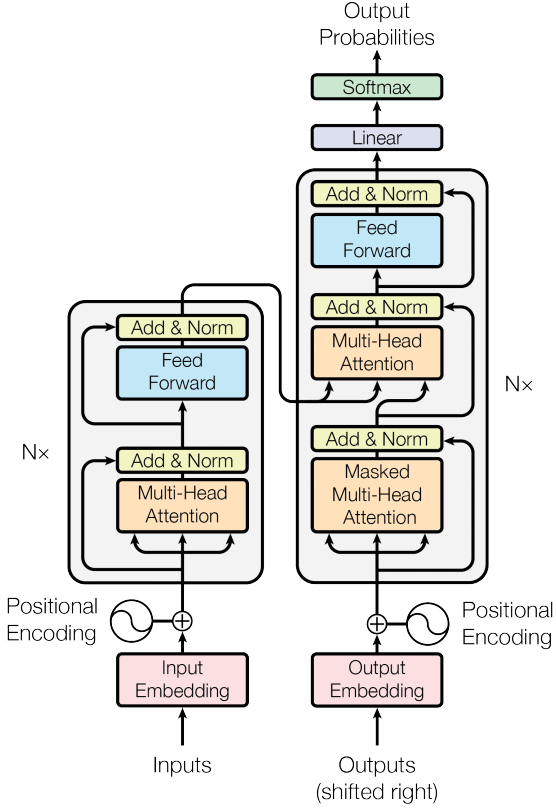
\includegraphics[width=.4\textwidth]{pics/Transformer.png}
	\caption{Architecture of Transformer}
	\label{fig:transformer}
\end{figure}

\begin{itemize}
	\item 由于Transformer没有循环结构, 但是加入了Positional Encoding
	\item 编码部分最终的输出. 会作为Decoder Block中Attention的$K, V$, 解码器的输入作为$Q$
	\item Decoder Block中的Masked Multi-head Attention, 处理当前输入时只允许看到当前位置之前的输入
	\item 在编码器中, 也有mask. 因为通常对输入进行padding
\end{itemize}

\subsubsection{一些关于Transformer的问题}
\paragraph{1.}{\textbf{为什么输入$X$要经过变换得到$Q, K, V$? 为什么不直接使用$X$?}}

如果直接使用$X$, 则$X$直接承担了三种角色: 查询、键和值. 难以学习到满足要求的$X$. 经过变换后得到的$Q, K, V$, $Q$负责表示查询的问题, $V$表示输入的信息, $K$表示与输入相关的“关键词”, $Q, K$相乘用于衡量查询的问题与各条信息之间的相似性. 

\subsection{BERT}
\begin{figure}[h] 
	\centering
	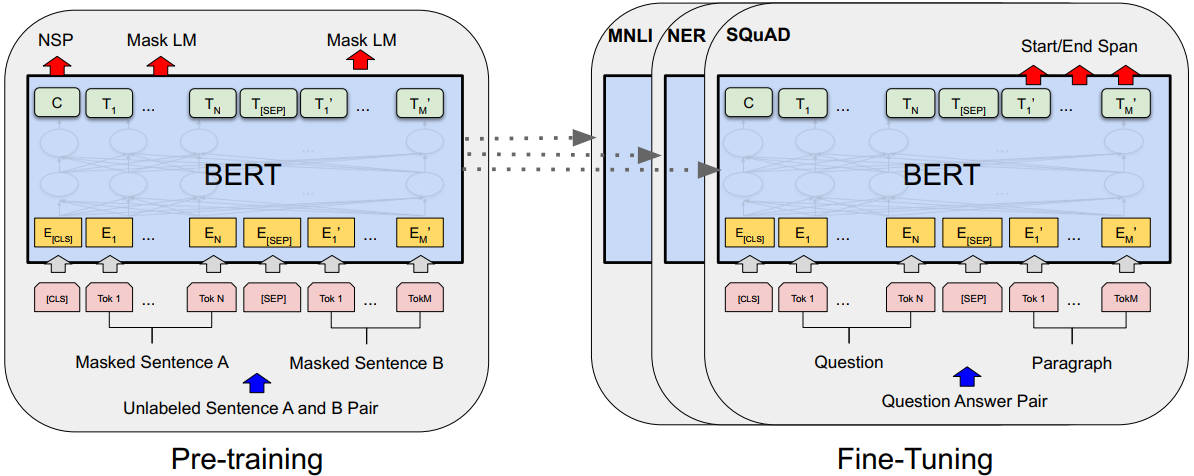
\includegraphics[width=.9\textwidth]{pics/bert-pre training-fine tunning.jpg}
	\caption{Overall pre-training and fine-tuning procedures for BERT}
	\label{fig:bert-pf}
\end{figure}

\paragraph{Motivation}
BERT(Bidirectional Encoder Representations from Transformers)\cite{devlin2019bert}缘自Transformer模型的编码器. 通常的语言模型都是单向的, 例如从左到右, 这使得在处理每个token时只能利用其之前的token. 单向的模型处理token-level的任务时, 难以应用到上下文的信息. 

\paragraph{HOW?}
BERT在大量无标签的文本数据集进行预训练, 得到模型的参数后, 再添加具体任务相关的神经网络层, 微调后即可得到适用于具体任务的模型, 即: pre-training + fine-tuning. 

\par{\textbf{Pre-training}}\ \ \ \ 在预训练阶段, BERT 在大量无标记的的数据上进行训练.  BERT使用两个预训练任务. 
\begin{myitemize}
	\item \textbf{Masked LM}(MLM). 随机 mask 一定比例的输入 tokens, 然后预测这些被 mask 的 tokens. 在最后一层被 mask 的 token 的表征被用于进行预测. 关于 masked tokens 的选择: 随机选择 15\% 的 tokens 被选中, 对于每个被选中的 token, 有 80\% 被替换为 \mintinline{python}{[MASK]}, 有 10\% 被替换为一个随机的 token, 有 10\% 保持不变. \textcolor{red}{为什么要这样做呢?} MLM 的一个负面影响是 pre-training 和 fine-tuning 间的\textbf{不匹配}. 这里的不匹配指的是: \mintinline{python}{[MASK]} 只会在预训练阶段出现, 而不会在微调阶段出现. 若 masked 的 tokens 只用 \mintinline{python}{[MASK]} 表示, 则会使得模型对 \mintinline{python}{[MASK]} 很敏感, 而对其他 token 不敏感. \textbf{计算损失时只在 masked tokens 上进行计算};
	
	\item \textbf{Next Sentence Prediction}(NSP). 这一任务是为了帮助模型理解句子之间的关系. 这一任务是给定两个句子 A, B, 预测 B 是否是 A 的下一个句子. 在这一任务中, 输入的形式是这样的: \mintinline{python}{[CLS] tokens of sentence1 [SEP] tokens of sentence2}. 在最后一层, \mintinline{python}{[CLS]} 的表征被用于进行预测. 这一任务在问答和自然语言推理中都很重要.
\end{myitemize}

\par{\textbf{Fine-tuning}}
预训练结束后就可以用模型来处理下游任务了. BERT 的下游任务的输入有的是单个文本有的是一对文本且输出也可能是不一样的. 针对每个任务, BERT 通过任务特有的输入输出模块来处理. 主要的一些下游任务有: 句子分类(情感分类), token 级别的分类(如词性预测), 两个句子作为输入的预测(例如两个句子之间是否有逻辑关系), 问答任务(例如输入是一篇文章和一个问题, 输出答案在文章中的位置). 

BERT 中\textcolor{red}{可能存在的一些问题}: 1) \mintinline{python}{[MASK]} 在实际预测中并不会出现, 训练时过多的 \mintinline{python}{[MASK]} 会影响模型的表现. 2) 由于每个 batch 中只有 15\% 的数据参与训练, 因此收敛会慢一些.

\begin{figure}[h] 
	\centering
	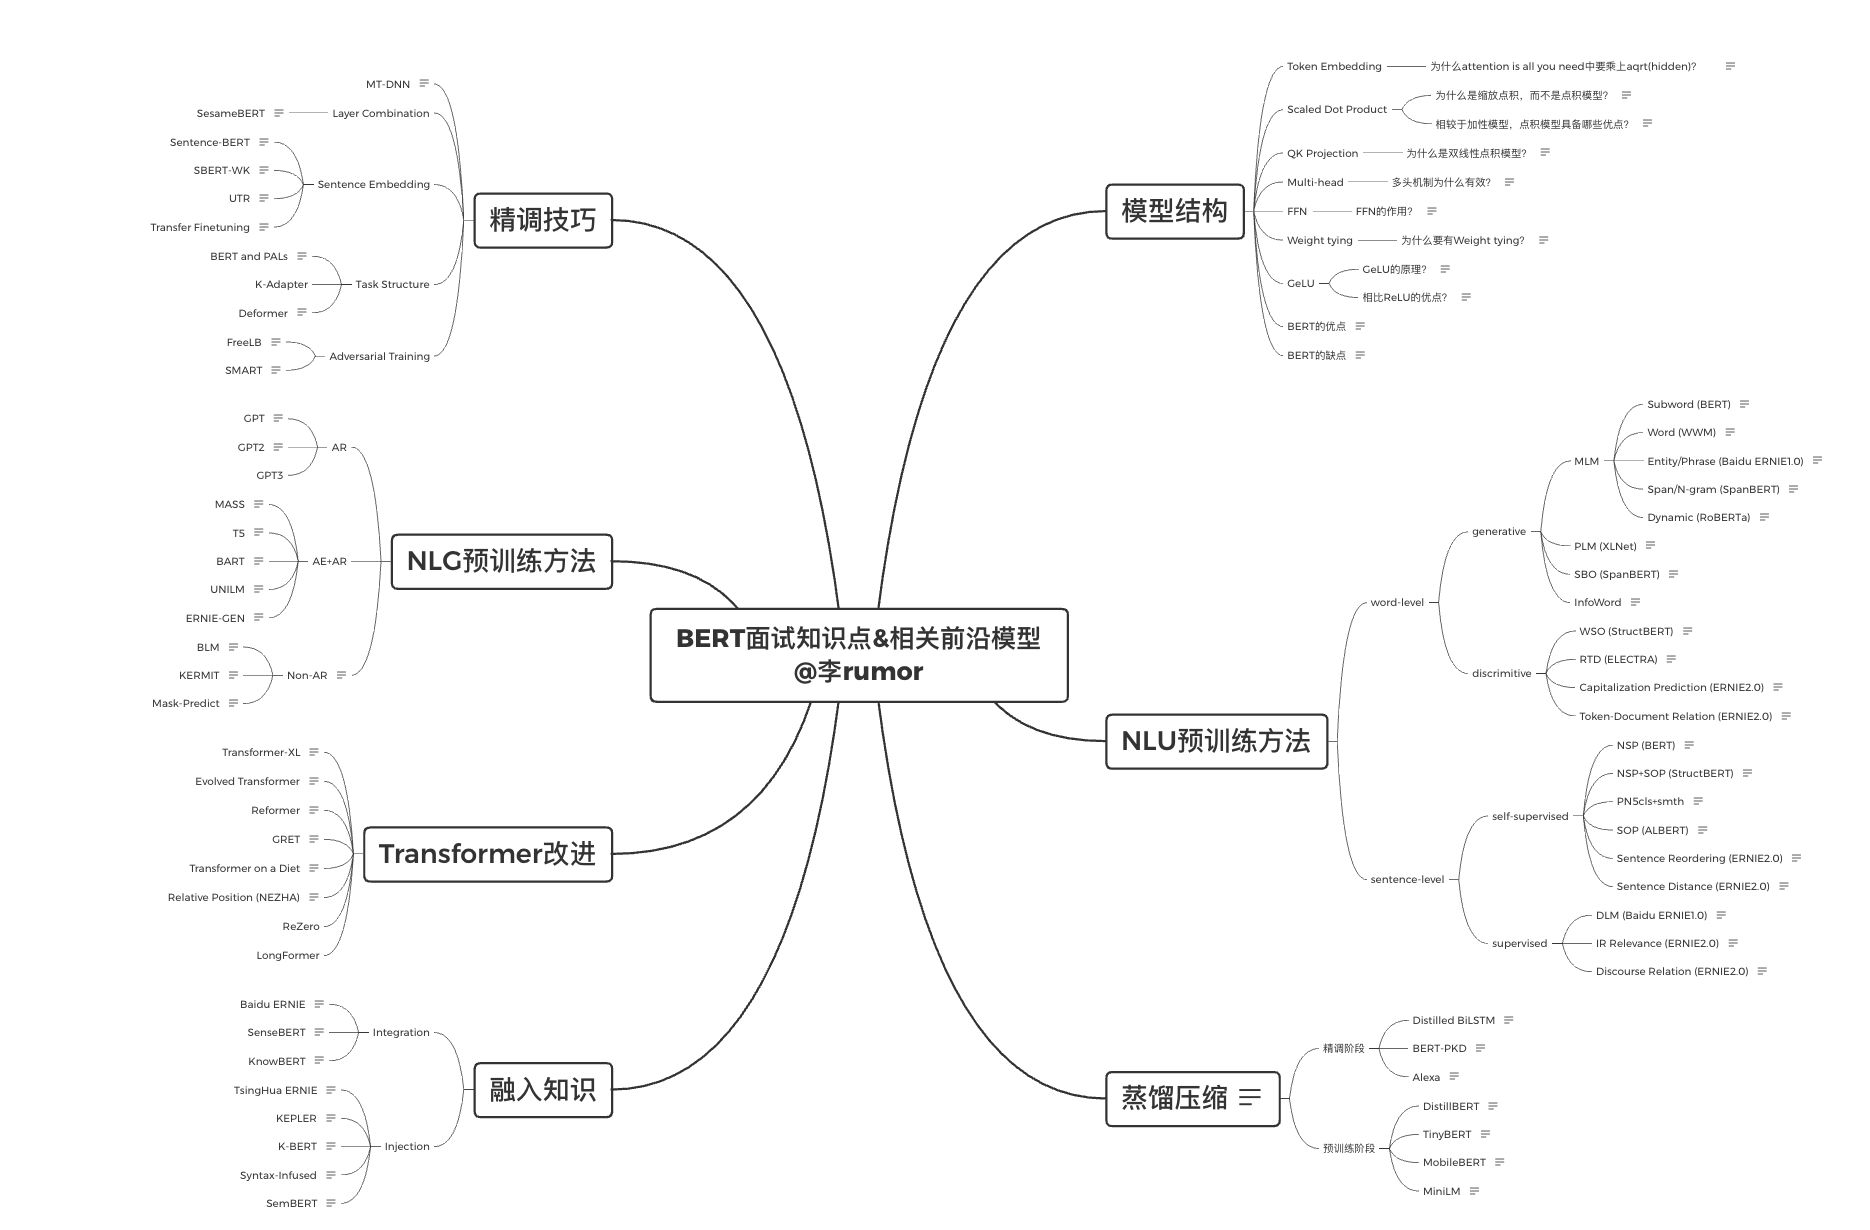
\includegraphics[width=1.1\textwidth]{pics/bert-roadmap.jpg}
	\caption{BERT 知识点总结(\href{https://zhuanlan.zhihu.com/p/46652512}{来源})}
	\label{fig:bert-roadmap}
\end{figure}

参考: \href{https://cloud.tencent.com/developer/article/1666168}{BERT详解(附带ELMo、GPT介绍)}.

\subsection{NeZha}
NeZha\cite{junqiu2019nezha}是华为在预训练模型上的实践总结, 它在BERT的基础上加了很多当下有用的优化, 比如Functional Relative Positional Encoding、Whole Word Masking策略、混合精度训练和LAMB优化器. 实验表明, NeZha在多项具有代表性的中文NLU任务上均取得了不错的成绩. NeZha的模型结构与Bert一致. 
\paragraph{Functional Relative Positional Encoding}有两种对位置进行编码的常用方案: 1)functional PE, 使用正余弦函数来对位置进行编码;2)Parametric PE, 将位置编码作为模型学习的参数. 后续又提出了相对位置编码, NeZha中使用了函数式的相对位置编码. 常用函数是的位置编码: 
$$
\begin{equation}\nonumber
	\left\{\begin{aligned}&\boldsymbol{p}_{k,2i}=\sin\Big(k/10000^{2i/d}\Big)\\ 
		&\boldsymbol{p}_{k, 2i+1}=\cos\Big(k/10000^{2i/d}\Big) 
	\end{aligned}\right.
\end{equation}
$$
其中其中$\boldsymbol{p}_{k,2i}, \boldsymbol{p}_{k,2i+1}$分别是位置$k$的编码向量的第$2i, 2i+1$个分量, $d$是位置向量的维度. 则计算Attention时: 
$$
\begin{equation}\nonumber
	\left\{
	\begin{aligned} 
		\boldsymbol{q}_i =&\, (\boldsymbol{x}_i + \boldsymbol{p}_i)\boldsymbol{W}_Q \\ 
		\boldsymbol{k}_j =&\, (\boldsymbol{x}_j + \boldsymbol{p}_j)\boldsymbol{W}_K \\ 
		\boldsymbol{v}_j =&\, (\boldsymbol{x}_j + \boldsymbol{p}_j)\boldsymbol{W}_V \\ 
		a_{ij} =&\, \frac{e^{ij}}{\sum_k e^{ik}}\\ 
		e_{ij} =& \frac{\boldsymbol{q}_i \boldsymbol{k}_j^T}{\sqrt{d}}\\
		\boldsymbol{o}_i =&\, \sum_j a_{i,j}\boldsymbol{v}_j 
	\end{aligned}\right.
\end{equation}
$$

引入相对位置编码后, 去掉原来的绝对位置编码$\boldsymbol{p}_k$, 分别引入相对位置的$key, value$编码$\boldsymbol{R}_{ij}^K, \boldsymbol{R}_{ij}^V$, 其中$i, j$分别表示序列中元素的位置. 则$\boldsymbol{q}_i$不变, $\boldsymbol{k}_i, \boldsymbol{v}_i$改变, 新的公式如下: 
$$
\begin{equation}\nonumber
	\left\{
	\begin{aligned} 
		\boldsymbol{q}_i =&\, \boldsymbol{x}_i \boldsymbol{W}_Q \\ 
		\boldsymbol{k}_j =&\, \boldsymbol{x}_j \boldsymbol{W}_K + \boldsymbol{R}_{ij}^K \\ 
		\boldsymbol{v}_j =&\, \boldsymbol{x}_j \boldsymbol{W}_V + \boldsymbol{R}_{ij}^V \\ 
		a_{ij} =&\, \frac{e^{ij}}{\sum_k e^{ik}}\\ 
		e_{ij} =& \frac{\boldsymbol{q}_i \boldsymbol{k}_j^T}{\sqrt{d}}\\
		\boldsymbol{o}_i =&\, \sum_j a_{i,j}\boldsymbol{v}_j 
	\end{aligned}\right.
\end{equation}
$$

在一些Parametric relative PE中, $\boldsymbol{R}_{ij}^K, \boldsymbol{R}_{ij}^V$是通过学习得到的, NeZha中通过正余弦函数计算得到: 

\begin{equation}
	\begin{aligned}
		\boldsymbol{R}_{ij}[2 k] =& \sin \left((j-i) /\left(10000^{\frac{2 \cdot k}{d_{z}}}\right)\right) \\
		\boldsymbol{R}_{ij}[2 k+1] =& \cos \left((j-i) /\left(10000^{\frac{2 \cdot k}{d_{z}}}\right)\right)
	\end{aligned}
\end{equation}

NeZha中$\boldsymbol{R}_{ij}^K, \boldsymbol{R}_{ij}^V$是相等的. 

\paragraph{Whole Word Masking}
在BERT中, 是对token进行随机mask的, 但是在中文预料中, 因为通常会进行分词, 所以一个词可能分成了多个token, 若其中一个token被mask, 其他的属于该词的token也应该被mask. mask的概率与BERT一致. 

\paragraph{Mixed Precision Training}
通常模型中的参数和梯度都是保存在32位浮点数. 在NeZha中使用了混合的精度. 在模型的每一次计算过程中, 维护一个32位的权重副本, 然后将其舍入为16位, 再用舍入后的权重进行前向和反向计算, 得到16位的梯度后, 将梯度转为32位, 再用32位的梯度与32位的权重副本来更新权重. 

\paragraph{LAMB Optimizer}
LAMB优化器为大batch-size的训练而生, batch大小可达30000!!!


\subsection{词嵌入模型}
\subsubsection{Word2Vec}

\subsubsection{fastText}
fastText 是 Facebook 于 2016 年提出的一个文本表示及分类方法 / 工具 (官方博客\href{https://fasttext.cc/blog/2016/08/18/blog-post.html}{Releasing fastText}). fastText 相关的主要参考文献: \cite{armand_fasttext_2016}, \cite{piotr_fasttext_2017}. 结合网上的一些资料以及看了相关论文后, 其实 fastText 更多的是一个构建在 word2vec 上的词向量学习和文本分类的工具. 其与 word2vec 较大的区别在于: 以文本分类作为目标训练词向量, 将词表示成 \textit{n-grams}, 词向量等于其 \textit{n-grams} 向量的和. 

\cite{piotr_fasttext_2017} 中以 \textit{skip-gram} 的形式训练, 且将目标函数从似然函数替换为了 \textit{logistic loss}:

$$
\log (1+e^{-s(w_t, w_c)}) + \sum_{n \in \mathcal{R}_{t,c}} \log (1+e^{s(w_t, n)})
$$

其中 $s(\cdot, \cdot)$ 是一个打分函数, 相当于计算两个词的相似性, 在文中定义为:

$$
s(w, c) = \sum_{g \in \mathcal{G}_w} \boldsymbol{z}_g^T \boldsymbol{v}_c
$$

其中 $\mathcal{G}_w$ 表示词 $w$ 对应的 \textit{n-grams} 集合.

\subsubsection{ELOM}


\subsection{Tokenization}
Tokenizer的目的是: 将文本处理为可以被模型处理的数据. 通常在文本相关的任务中会将文本处理为更细的粒度, 如将篇章处理为句子、句子处理为word、word处理为token, 甚至可以将token处理为character. Tokenizer将文本转化为token, 并基于token表将token转为数字. 常用的tokenization方法: 
\subsubsection{word-based}
一个直接的方法便是以word为token. 通常来说, 可以制定一些规则将文本划分为word序列, 例如英语语料可用空格分割. 但是容易产生以下几个问题: 
\begin{myitemize}
	\item 最终的词汇表可能会非常大
	\item 十分相似的词, 会得到没有关联的id. 如dog和dogs, 被在词汇表中表示为两个词, 但二者的id没有关联, 并不能反映二者真实的语义关系. 这种情况也是使得词汇表庞大的原因之一. 当然, 可以制定规则处理这些情况, 但是还有一些情况难以处理, 如有相同词根的词
	\item 有些词可能会因为时态、词缀等的变化而被视作不同的词, 这也加大了OOV(out of vocabulary)出现的概率	
\end{myitemize}

\subsubsection{character-based}
显然, 这种方法是把原始文本用字符来表示. 这种方式适用于英文, 也适用于中文, 不需要进行分词. 有两个明显的有点: 

\begin{myitemize}
	\item 词汇表会小很多
	\item 出现OOV的概率基本可以消除
\end{myitemize}

但也带了一些很明显的问题: 

\begin{myitemize}
	\item 语义不明显. 将文本分散为character后, 单个character含有的语义太过零散
	\item 处理后的文本包含的token过多, 不利于输入模型, 通常模型的输入是有长度限制的
\end{myitemize}

\subsubsection{subword}
Subword, sub-word, 比我们平常所用的word更小的word, 通常为word的一部分. Subword tokenization的一个原则: 频繁出现的word不应该拆分成sub-word, 而不频繁出现的word应该被分解为更小的、更频繁出现的sub-words. 这种方式可以将较长的word、少见的word分解为常用的sub-words, 且sub-word可以被不同的word之间共享. 


\subsection{BIM}
binary independence model, 二元独立模型. BIM 是一种计算查询与文档相关性的方法. 这种方法通常用在搜索的文档列表排序中, 依据相关性进行排序. BIM 有两个基本假设: 
\begin{itemize}
	\item \textbf{二元假设}: 类似于布尔模型中的文档表示方法, 一篇文档在由特征 (或者单词) 进行表示的时候, 以特征 (或者单词) 出现和不出现两种情况来表示, 不考虑词频等其他因素;
	
	\item \textbf{词汇独立性假设}: 指文档里出现的单词之间没有任何关联, 任意一个单词在文档的分布概率不依赖于其他单词是否出现. 因为词汇之间没有关联, 所以可以将文档概率转换为单词概率的乘积.
\end{itemize} 

\subsubsection{概率检索模型}
一种直接对用户需求进行相关性建模的方法. 对于用户给出的 \textit{query}, 将所有文档分为两类: 相关文档和不相关文档 (\textcolor{red}{如何划分为相关与不相关}). 对于文档 $D$ 来说, $P(R|D)$ 表示文档相关的概率, $P(NR|D)$ 表示文档不相关的概率. 相关性的目标是判断 $P(R|D) > P(NR|D)$ 是否成立. 根据贝叶斯公式转化可得: $\frac{P(D \mid R)}{P(D \mid N R)}>\frac{P(N R)}{P(R)}$. $P(D|R)$, $P(D|NR)$ 表示在相关/不相关文档中观察到 $D$ 的概率. 在排序时并不需要真的分类, 只需要保证相关性由低到高排序即可, 即按照 $\frac{P(D \mid R)}{P(D \mid N R)}$ 降序排序.

\subsubsection{BIM 的推导}
BIM 计算主要集中在上述的两个因子: $P(D|R)$ 和 $P(D|NR)$ 的计算.

根据 BIM 的二元假设, 文档 $D$ 可以表示为一个 0/1 向量, 假设 $D = \{1, 0, 1, 0, 1\}$, 1 表示对应的词出现在 $D$ 中. 用 $p_i$ 表示词汇表中第 $i$ 个单词在相关文档中出现的概率, \textbf{则在已知相关文档集合的情况下}, 观察到 $D$ 的概率为:
$$
P(D|R) = p_1 \times (1-p_2) \times p_3 \times (1-p_4) \times p_5
$$

用 $s_i$ 表示第 $i$ 个单词出现在不相关文档中的概率, 则在不相关文档中观察到 $D$ 的概率为:
$$
P(NR|D) = s_1 \times (1-s_2) \times s_3 \times (1-s_4) \times s_5
$$

\textbf{注意}: $p_i, s_i$ 表示的是第 $i$ 个词在相关 / 不相关文档中出现的概率, 很显然\textbf{在已知相关 / 不相关文档的情况下}, $p_i$可以通过计算在相关文档中有多少文档包含了第 $i$ 个词来计算, $s_i$ 同理.

那么, 可以得到
$$
\frac{P(D \mid R)}{P(D \mid N R)}=\frac{p_{1} \times\left(1-p_{2}\right) \times p_{3} \times\left(1-p_{4}\right) \times p_{5}}{s_{1} \times\left(1-s_{2}\right) \times s_{3} \times\left(1-s_{4}\right) \times s_{5}}
$$
对其进行推广后:
$$
\frac{P(D \mid R)}{P(D \mid N R)}=\prod_{i: d_{i}=1} \frac{p_{i}}{s_{i}} \times \prod_{i: d_{i}=0} \frac{1-p_{i}}{1-s_{i}}
$$
其中 $d_i=1$ 表示文档中出现了的单词, $d_i=0$ 没有出现在文档中. 对上式进行变换:
$$
\begin{aligned}
	\frac{P(D \mid R)}{P(D \mid N R)} &=\prod_{i: d_{i}=1} \frac{p_{i}}{s_{i}} \times\left(\prod_{i: d_{i}=1} \frac{1-s_{i}}{1-p_{i}} \times \prod_{i: d_{i}=1} \frac{1-p_{i}}{1-s_{i}}\right) \times \prod_{i: d_{i}=0} \frac{1-p_{i}}{1-s_{i}} \\
	&=\left(\prod_{i: d_{i}=1} \frac{p_{i}}{s_{i}} \times \prod_{i: d_{i}=1} \frac{1-s_{i}}{1-p_{i}}\right) \times\left(\prod_{i: d_{i}=1} \frac{1-p_{i}}{1-s_{i}} \times \prod_{i: d_{i}=0} \frac{1-p_{i}}{1-s_{i}}\right) \\
	&=\prod_{i: d_{i}=1} \frac{p_{i}\left(1-s_{i}\right)}{s_{i}\left(1-p_{i}\right)} \times \prod_{i} \frac{1-p i}{1-s_{i}} \\
	&=\prod_{i: d_{i}=1} \frac{p_{i}\left(1-s_{i}\right)}{s_{i}\left(1-p_{i}\right)}
\end{aligned}
$$
上式中的第三步 $\prod_{i} \frac{1-p i}{1-s_{i}}$ 是一个与文档无关的量, 因此对同一个 \textit{query} (相关/不相文档划分) 来说, 是不影响文档与 \textit{query} 的相关性排序的, 故可以省去. 对上式的结果取 $\log$:
$$
\log \left(\frac{P(D \mid R)}{P(D \mid N R)}\right)=\sum_{i: d_{i}=1} \log \frac{p_{i}\left(1-s_{i}\right)}{s_{i}\left(1-p_{i}\right)}
$$
接下来的重点就是如何估计 $p_i$, $s_i$ 了, 如前文所述, 只需要统计每个词在相关 / 不相关文档集合中出现的频率即可:
$$
\begin{array}{llll} 
	& \text { 相关文档 } & \text { 不相关文档 } & \text { 文档数量 } \\
	\hline d_{i}=1 & r_{i} & n_{i}-r_{i} & n_{i} \\
	d_{i}=0 & R-r_{i} & (N-R)-\left(n_{i}-r_{i}\right) & N-n_{i} \\
	\hline \text { 文档数量 } & R & N-R & N
\end{array}
$$
因此, $p_i = \frac{r_i + 0.5}{R+1}$, $s_i = \frac{(n_i - r_i) + 0.5 }{(N - R) + 1}$, 其中 0.5 是引入了平滑项以避免为 $\log 0$. 那如何在给定 \textit{query} 的情况下利用以上的内容对文档进行排序呢? 如下:
$$
\text{rel(query, D)} = \sum_{q_{i}=d_{i}=1} \log \frac{\left(r_{i}+0.5\right)\left((N-R)-\left(n_{i}-r_{i}\right)+0.5\right)}{\left(n_{i}-r_{i}+0.5\right)\left(R-r_{i}+0.5\right)}
$$
该式表示 \textit{query} 与 $D$ 的相关性, 其物理意义: 对于同时出现在 \textit{query} 和 $D$ 中的词, 累加每个单词对相关性的贡献, 和就是总的相关性, 于是就可以以此来对文档进行排序了. \textbf{\textcolor{red}{在不确定哪些文档是相关的, 哪些文档是不相关的的时候, 可以给公式的估算因子直接赋予固定值, 则该公式将会退化为IDF因子}}. 例如依从最大熵的原理假设 $p_i = 0.5$, 且相关文档与不相关文档相比只占极小部分, 则可得 $\log \frac{p_i (1 - s_i)}{(1 - p_i) s_i} = \log \frac{1 - s_i}{s_i} = \log \frac{N - n_i + 0.5}{n_i + 0.5} \approx IDF_i$. 所以, \textbf{一个比较关键的问题是如何估计 $p_i, s_i$}, 实际中可以通过用户的点击来估计.

BIM 的缺点也很明显: 只考虑了词是否出现, 不考虑词频对相关性的影响, 忽略了文档长度的影响, 且与现在的深度学习模型相比, 容易因为同义但不相同的词而错过相关的文档.

参考的资料: \href{https://www.cnblogs.com/bentuwuying/p/6730891.html}{概率检索模型: BIM+BM25+BM25F}, \href{https://blog.csdn.net/SrdLaplace/article/details/84954920}{基于词相关性的排序算法}.

\subsection{BM25}
Best Match25. BM25 算法实质上是一个用于信息检索中, 对给定查询 (query) 和若干 "相关" 文档 (document) 进行相关性排序打分的排序函数. BM25 算法其\textbf{主要思想}可简述如下: 对 \textit{query} 进行特征提取分解, 生成若干特征项 (词) $q_i$; 然后对于每个搜索结果文档 $D$, 计算每个特征 $q_i$ 与 $D$ 的相关性得分; 最后将 $q_i$ 相对于 $D$ 的相关性得分进行加权求和, 从而得到 \textit{query} 与 $D$ 的相关性得分. 其计算公式:
$$
\operatorname{score}(\text{query}, D)=\sum_{i} W_{i} \cdot R\left(q_{i}, D\right)
$$
其中 $W_i$ 表示 $q_i$ 的权重, $R(q_i, D)$ 是 $q_i$ 与 $D$ 的相关性得分. 接下来就是如何计算 $W_i$ 和 $R(q_i, D)$ 了. 当然, 在实际使用时, 它们的定义或许并不和下面描述的完全一样.

\subsubsection{$W_i$}
一个词的权重可以有很多衡量方式, 一些传统的方法大多是基于统计来计算的, 比较常用的有 Robertson-Sparck Jones IDF:
$$
\operatorname{IDF}\left(q_{i}\right)=\log \frac{N-n\left(q_{i}\right)+0.5}{n\left(q_{i}\right)+0.5}
$$
其中 $n(q_i)$ 是文档集中包含 $q_i$ 的文档的数量. 可以注意到, 这个式子与上一节的 BIM 结尾处举的例子是一样的, 这种情况值得是初始状态我们不知道哪些文档是相关的, 且相关文档的占比通常是极小的. 所以可以认为 BM25 的权重使用的是特殊情况下的 BIM. $W_i$ 有一个问题还需要注意, 当 $n(q_i)$ 超过 $N$ 的一半时, $W_i$ 就变成负的了, 因此实际使用时通常将这种情况下的 $W_i$ 置为 0.


\subsubsection{$R(q_i, D)$}
一些比较朴素的定义: 特征词在文档中的频率. 但是这种方法难以避免文本长度的影响, 即长文本通常会有更高的词频, 类似于推荐中的热门物品. 还有一个问题就是 $R$ 并不应该与词频是线性关系的, 而应该是增长到一定程度就趋于饱和, 这样就不会\textbf{让某个特征词占据支配地位}. 基于以上考虑, BM25 中的 $R$ 定义为:
$$
\begin{aligned}
	R\left(q_{i}, D\right) &=\frac{\left(k_{1}+1\right) \cdot \tilde{t} f\left(q_{i}, D\right)}{k_{1}+\tilde{tf}\left(q_{i}, D\right)} \\
	\tilde{t f}\left(q_{i}, D\right) &=\frac{t f\left(q_{i}, d\right)}{1+b\left(\frac{L_{D}}{L_{\text {avg }}}-1\right)}
\end{aligned}
$$
其中 $tf(q_i, D)$ 表示 $q_i$ 在 $D$ 中的词频, $L_d, L_{avg}$ 分别为 $D$ 的长度和所有文档的平均长度. $k_1, b$ 为参数, 一般取值范围为 $k_1 \in [1.2, 2.0], b=0.75$. 对上式进行化简:
$$
R(q_i, D) = \frac{(k_1+1) tf(q_i, D)}{k_1[(1 - b) + b \frac{L_D}{L_{avg}}] + tf(q_i, D)}
$$
$k_1$ 起着调节特征词与词频尺度的作用, 很显然, 当 $k_1=0$ 时则 $R$ 成了与词频无关的量, $k_1$ 越大则 $R$ 越接近原始的词频.

\subsubsection{特征词在 \textit{query} 中的重要性}
此外, 若 \textit{query} 比较长, 且某些特征词在 \textit{query} 中的频率比较高, 则这些特征词的重要性也应该提高, 但应该其重要性的提高也应与特征词在文档中重要性一样, 其\textbf{增长也是会饱和的}. 因此在 $score$ 中加入这一项:
$$
R(q_i, query) = \frac{(k_3 + 1) \cdot tf(q_i, query)}{k_3 + tf(q_i, query)}
$$
可以看出这和 $R(q_i, D)$ 是很相似的, $k_3$ 与 $k_1$ 的作用类似, 但是 $R(q_i, query)$ 中没有考虑

BM25 的\textbf{缺点}: 显然, BM25 其实就是 \textit{query} 中每个词与文档的相关性的加权求和, 这一过程肯定是损失了一部分信息的, 如 $q_i$ 之间的顺序关系. 

所以, 最终得到:
$$
score(query, D) = \sum_{i} \log \frac{N-n\left(q_{i}\right)+0.5}{n\left(q_{i}\right)+0.5} \cdot \frac{(k_1+1) tf(q_i, D)}{k_1[(1 - b) + b \frac{L_D}{L_{avg}}] + tf(q_i, D)} \cdot \frac{(k_3 + 1) \cdot tf(q_i, query)}{k_3 + tf(q_i, query)}
$$
其实看这个式子有一个问题, 就是\textbf{\textcolor{red}{特征词在 \textit{query} 中的重要性与文档是无关的, 这样对排序还有用吗?}}

BM25 的\textbf{缺点}: BM25 将文档当作一个整体来进行词频统计 (计算 $R$), 但是显然一个文档的不同部分对 $R$ 的贡献是不等的. BM25 的一些变体对此进行了改进, 如 BM25F 在计算 $R$ 时将文档分割成不同的区域来进行加权统计

参考资料: \href{https://www.cnblogs.com/geeks-reign/p/Okapi_BM25.html}{Okapi BM25算法}(很详细), \href{https://www.cnblogs.com/bentuwuying/p/6730891.html}{概率检索模型: BIM+BM25+BM25F}, \href{https://www.cnblogs.com/NaughtyBaby/p/9774836.html}{BM25 调参调研}(探讨了 BM25 中的参数的影响).

\subsection{Word2Vec}



\clearpage
\part{Recommender Systems}
{\noindent}	 \rule[-10pt]{17.5cm}{0.5em}\\
\section{基本概念}
\subsection{历史背景}
\paragraph{Motivation}互联网的发展, 人们接受的信息越来越多, 从信息稀缺时代逐渐过渡到了信息爆炸时代. 面对数据的海洋, 我们越来越希望我们感兴趣的信息能够直接呈现在我们面前. \tbc{red}{把用户想要的信息推荐给用户} --- 推荐系统的宗旨. 

\paragraph{发展过程}: 
\begin{itemize}
	\item 1994年, 明尼苏达大学GroupLens研究组推出第一个自动化推荐系统GroupLens, 提出将协同过滤作为推荐系统的重要技术
	\item 1995年, 卡耐基梅隆大学的Robert Armstrong等人提出个性化导航系统Web Watcher;斯坦福大学的Marko Balabanovic等人退出了个性化推荐系统LIRA
	\item 1997年, Resnick等人首次提出Recommender System一词
 	\item 1998年, Amazon上线了基于物品的协同过滤算法, 并在千万级用户和百万计商品的规模上进行了应用. Amazon于2003年发表论文\cite{linden2003amazon.com}公布了基于物品的协同过滤算法
	\item 2001年, IBM在其电子商务平台Websphere中增加个性化功能
	\item 2003年, Google开创AdWords盈利模式, 通过用户的广告词来提供相关的广告. 2007年Google为AdWords添加个性化元素, 通过对用户一段时间内的搜索历史进行记录和分析, 以便更精准呈现广告
	\item 2006年, Netflix宣布一项竞赛, 任何人只要能将其现有的电影推荐算法Cinematch的预测准确度提高10\%就能获得100万美金
	\item 2007年, Yahoo提出SmartAds广告方案, 通过分析用户信息以及用户搜索、浏览行为为用户呈现个性化广告
	\item 2007年, 第一届ACM推荐系统大会举行
	\item 2015年, Facebook在其官网公布了其推荐系统原理、性能及使用情况(\href{https://engineering.fb.com/2015/06/02/core-data/recommending-items-to-more-than-a-billion-people/}{Recommending items to more than a billion people}), 相关论文\cite{he2014practical}
	\item 2016年, YouTube发表论文\cite{covington2016deep}介绍Youtube如何向用户推荐个性化的视频
	\item 2016年. , Google发表论文\cite{cheng2016wide}介绍App商店中的推荐系统, 即Wide\&Deep 模型
\end{itemize}

形式上来看, 推荐系统的任务是这样的: 给定一个输入, 从数据集中搜索出一系列数据对象, 并排序后输出. 

输入通常是关于某个用户的表示, 可以是该用户的特征、向量化的表征等, 除此之外用户的行为数据, 如用户的浏览记录、搜索记录、与商品的交互数据、用户的一些动态变化的数据等都可以与用户特征一起作为输入, 而待搜索的数据集中通常是商品的数据, 如商品的特征等, 基于以上丰富的信息, 将输入的信息与数据集中对象进行匹配, 给出推荐的顺序. 

乍一看, 这和搜索很像. 其实这么说也没错, 都是一个\tbc{red}{Learning To Rank}的任务. 其实很多领域研究的问题都很相似, 通过进一步的抽象可以看作是同一个问题. 但随着研究的深入, 为了在一个问题上取得更好的效果, 会相应地结合该领域地特点, 如领域内特有的信息、领域内特有的数据形式等. 因此, 虽然问题之间有重叠, 但为了做得更好, 除了基础的方法, 还需要更深入地挖掘领域地特点!例如, 在推荐系统中, 用户的需求和兴趣是隐含的(隐含在历史数据中, 可能用户都不知道自己喜欢什么), 而搜索中搜索语句是显式的(用户需求是明确的). 

\paragraph{推荐系统主要元素}
\begin{itemize}
	\item 物品集合: 被推荐的物品或内容
	\item 用户: 用户的基本信息, 如基本信息、行为信息、兴趣爱好等
	\item 场景: 用户所处的环境, 如网络环境、所处位置等
	\item 推荐引擎: 根据用户对物品的偏好与用户的画像数据进行拟合, 学习什么样的用户会喜欢什么样的物品. 引擎包含以下重要模块: 
	\begin{itemize}
		\item 召回模块: 根据用户和场景特征, 从整个物品数据集(上百万物品)中挑选用户可能感兴趣的物品, \textbf{挑选出一个较小的候选集}(几百至几千). 召回模块中, 通常使用简单的特征进行快速查询, 比如用户最近点击的物品的相似物品、根据用户兴趣召回物品等. 常用的算法: Word2vec、LDA、LSTM、ItemCF、UserCF、DNN等
		\item 排序模块: 针对召回模块找到的\textbf{候选集进行精排}, 得到用户对候选物品集的评分. 常用的算法: LR、FM、XGBoost、GBDT+LR、Wide\&Deep、FNN、PNN、DeepFM、NFM、DIN等
		\item 后排模块: 得到用户对候选集的评分后, 可以根据一些规则对排序进行调整, 如运营干预、优先级调权等
	\end{itemize}
	\item 推荐结果集: 推荐结果, 或推荐结果的有序排列
\end{itemize}

\subsection{会话推荐}
会话推荐 (session-based recommendation) 是预测用户在一条交互序列中可能会喜欢的下一个商品. 基于深度学习的会话推荐方法试图从用户的历史交互序列中学习和理解用户的行为, 建模用户的偏好. Session-based Recommender System (SBRS) 是指在用户未登录状态下, 仅仅依赖匿名会话进行用户下一个行为预测的一种算法, 在许多领域(如电商、短视频、直播等)有着重要的作用. SBRS 从用户与系统交互过程中的会话来学习用户的偏好. 每一个会话由一段连续的时间内用户与物品的若干个交互组成, 例如在一次网购中所购买的商品.

近期 SBRS 的 SOTA 结果都是基于神经网络模型取得的. 
\begin{myitemize}
	\item 2016年提出的 GRU4Rec 是该系列中经典的一篇, 首次利用RNN对session序列建模, 相比传统的 KNN 和矩阵分解, 效果有明显的提升. GRU4Rec 的核心思想是在一个 session 中, 用户点击一系列 item 的行为看做一个序列, 用来训练 RNN 模型. 预测阶段, 给定已知的点击序列作为输入, 预测下一个可能点击的 item.;
	
	\item 在 GRU4Rec 的基础上, NARM 将注意力机制应用于对 session 的顺序行为及主要意图进行分别建模. 和以往方法不同的是显示地对用户在 session 目的进行建模;
	
	\item 与 NARM 相似, STAMP 利用简单的多层感知机和注意力网络对 session 内长短期兴趣分别表征. STAMP 设计了不同结构分别对 session 内长期兴趣和短期兴趣建模, 取序列中最后一个交互的item表征短期兴趣;
	
	\item 之前序列模型都仅对连续交互相邻 item 之间的序列过渡关系进行挖掘, 而忽略了不相邻 item 之间复杂地转变, SR-GNN 通过引入 GNN 来对 session graph 进行建模, 以此发掘序列内 item 之间复杂的过渡模式;
	
	\item 之前的方法通常忽略了 session 间的关系, GCE-GNN 提出了一种全局上下文增强(global-context enhanced)的 GNN 网络. 能够从两种层次来学习物品的表征, 包括 global-level: 从所有 session 构成的图上进行全局的表征;以及 session-level: 从单个 session 局部 item 转移图上进行局部的表征. 最后融合二者, 并通过注意力机制形成最终的序列表征, 用于序列推荐任务.
\end{myitemize}

\subsection{共现矩阵}
显然, 共现矩阵是一种矩阵, \textbf{关键是它描述了一种什么事实}?$M, N(|M| = m, |N| = 2)$表示两个相同或者不同的集合, 共现矩阵可以用于表达两个集合笛卡尔乘积的元素对的某种关系, $(m_i, n_j)$间的这种关系可以用共现矩阵的元素$CM_{ij}$表示. 

在具体的应用场景中, 
\begin{itemize}
	\item 推荐系统: $M$表示用户集, $N$表示商品集, $CM_{ij}$表示用户$m_i$对$n_j$的喜爱程度(如评分)、是否点赞、是否分享等
	\item 自然语言处理: $M = N$表示词汇表, $CM_{ij}$表示词$m_i$与词$m_j$出现在同一个句子中的次数
	\item 社交网络: $M=N$表示作者集合, $CM_{ij}$表示$m_i$与$m_j$间存在某种关系, 如朋友关系、合作关系等
\end{itemize}
共现矩阵是两个集合的元素间关系的一个很直白的表达. 正是因为直白, 共现矩阵通常很稀疏, 空间需求大. 

\subsection{召回方法分类}
召回即从海量的数据集中找出尽可能包含真实结果的候选集. 常见的分类: 
\begin{itemize}
	\item 行为相似召回: 通过用户与物品的交互行为, 发现行为指向的物品的相似物品
	\item 相似用户召回: 通过用户画像和用户行为等, 计算用户之间的相似性, 根据相似用户的行为进行召回物品
	\item 内容相似召回: 通过对物品内容进行分析, 得到物品之间的相似性, 根据与用户产生交互的物品来召回
\end{itemize}


\subsection{常用相似度计算方法}
\paragraph{同现相似度}
物品A和物品B的同现相似度: 
$$
w_{A,B} = \frac{|N(A) \cap N(B)|}{|N(A)|}
$$
其中, $A(A), N(B)$分别表示喜欢A和B的用户集合. 但是这种相似度有个问题, 当B是热门物品时, 喜欢A的用户中可能绝大部分也会喜欢B, 那么$w_{A,B}$就会接近于1, 即任何物品与热门物品的相似度都会接近于1. 除此之外, 还有个问题, 这个相似度不是对称的, 即$w_{A,B} \neg w_{B,A}$, 这看起来是有点不合理的, 因此, 其改进如下: 
$$
w_{A,B} = \frac{|N(A) \cap N(B)|}{\sqrt{|N(A)| \cdot |N(B)|}}
$$

\paragraph{欧几里得距离}
众所周知, 欧氏距离是欧氏空间中两点之间的距离. 两个物品A, B的向量表示为$\boldsymbol{V}_A, \boldsymbol{V}_B$, 则欧式距离为: 
$$
d(A, B) = ||\boldsymbol{V}_A - \boldsymbol{V}_B||_2
$$
以欧式距离计算A, B间相似性时可如下计算: 
$$
sim(A, B) = \frac{1}{1 + d(A, B)}
$$
或许还有其他的形式, 例如: 
$$
sim(A, B) = e^{-d(A, B)}
$$

\paragraph{皮尔逊相关系数}
介于-1和1之间, 它度量两个序列(可以是用户对物品的偏好/评分序列)之间的线性相关程度. 它度量数字一起按比例改变的倾向性, 也就是说两个数列中的数字存在一个大致的线性关系. 当该倾向性强时, 相关值趋于1. 当相关性很弱时, 相关值趋于0. 在负相关的情况下一个序列的值很高而另一个序列的值低---相关趋势趋于-1. 

使用皮尔逊相关系数计算用户/物品相似度时, 通常取共现矩阵中的行(用户对各个物品的偏好)或列(各个用户对一个物品的偏好)作为数列来计算皮尔逊相关系数. 两个物品/用户A, B的向量表示为$\boldsymbol{x}, \boldsymbol{y}$, 则皮尔逊相关系数为: 
$$
r_{\boldsymbol{xy}} = \frac{\sum_i (x_i - \bar{x})(y_i - \bar{y})}{\sqrt{\sum_i (x_i - \bar{x})^2} \sqrt{\sum_i (y_i - \bar{y})^2}}
$$
其实, 仔细一看, 皮尔逊相关系数和余弦相似度很像, 对$\boldsymbol{x}, \boldsymbol{y}$进行标准化后再进行余弦相似度计算. 皮尔逊相关系数用于计算相似性时有以下问题: 
\begin{itemize}
	\item 没有考虑序列的长短. 例如两个用户交互的物品的交集可能会比较大或较小, 通常交集较大的情况下更可靠, 但是交集更小时计算出的皮尔逊系数可能会更大
	\item 若序列长度为1时, 根据定义则无法计算皮尔逊系数
	\item 若序列中的值都相同时也无法计算皮尔逊系数, 因为方差为0
\end{itemize}


\paragraph{余弦相似度}
两个物品/用户A, B的向量表示为$\boldsymbol{V}_A, \boldsymbol{V}_B$, 则余弦相似度为: 
$$
sim(A, B) = \frac{\boldsymbol{V}_A \cdot \boldsymbol{V}_B}{||\boldsymbol{V}_A||_2 \times ||\boldsymbol{V}_B||_2}
$$

\paragraph{Jaccard系数}
两个物品/用户A, B的向量表示为$\boldsymbol{V}_A, \boldsymbol{V}_B$, 则Jaccard相似度为: 
$$
sim(A, B) = \frac{\boldsymbol{V}_A \cdot \boldsymbol{V}_B}{||\boldsymbol{V}_A||_2 + ||\boldsymbol{V}_B||_2 - \boldsymbol{V}_A \cdot \boldsymbol{V}_B}
$$


\subsection{推荐中要注意的点}
\begin{myitemize}
	\item 长尾效应: 位于长尾位置的曝光率低的项目产生的利润不低于只销售曝光率高的项目的利润. 注意对长尾物品的推荐效果, 热门物品的推荐较长尾物品更容易, 在评价算法效果时要注意对长尾物品的推荐效果
	\item 用户经常购买的物品并不一定能体现用户的偏好, 如很多人都会经常买卫生纸, 但这并不能体现用户很喜欢卫生纸, 卫生纸作为热门物品反而并不能体现用户的偏好. 不同的物品对用户的偏好的贡献是不一样的 --- \textbf{user-aware}
	\item 使用用户行为数据来预测某个用户对某个物品的评分时, 要注意历史行为中的物品起的作用可能是不同的\cite{he2018nais}. 如预测我会不会买iphone时, 可能与我过去买的是什么手机有关 --- \textbf{target item-aware}
	\item 如何对待用户没有交互过的物品?
\end{myitemize}

\subsection{常用指标}
此处介绍的指标不涉及具体的计算公式, 在不同的场景下有不同的具体定义, 计算自然也相应而变. 
\paragraph{覆盖率}覆盖率用来描述一个推荐系统对长尾内容或商品的发掘能力. 关于覆盖率的定义, 最简单的理解是推荐系统能够推荐出来的物品, 占平台中全部物品的比例. 

\paragraph{多样性}用户的兴趣是非常广泛的, 在一个视频应用中, 用户可能既喜欢看烧脑电影, 也喜欢看动作大片. 那么, 为了满足用户广泛的兴趣, 推荐列表需要能够覆盖用户不同的兴趣领域, 即推荐结果需要具有多样性. 想提升推荐系统的多样性, 就需要在较大的时间跨度上去识别和理解用户的兴趣. 

\paragraph{新颖性}新颖, 指给用户推荐那些他们以前没有听说过的内容或商品, 例如在视频应用中应该尽可能多地向用户推荐他们没有看过的电影. 而考虑到很多用户在某个应用中的使用粘性可能并不高, 例如一个用户可能同时是多个视频应用的用户, 所以仅仅依靠用户在自己系统中的行为记录来保证推荐的新颖性是不够的. 

除此之外比较简单方法是基于内容或商品的平均流行度去进行推荐, 因为越不热门的东西越可能让用户觉得新颖. 

不过, 向用户推荐不流行的内容或商品, 其实是牺牲了一定的推荐精度的, 所以我们需要权衡该指标与其它指标之间的平衡——这不仅在于技术层面的考量, 可能也在于商业层面的考量. 

\paragraph{惊喜度}如果推荐结果和用户的历史兴趣不相似, 但却能够让用户觉得满意, 那么就可以说推荐结果的惊喜度很高. 想要兼顾推荐系统的惊喜度并不是一件容易的事情, 因为这意味着需要降低推荐结果和用户历史兴趣的相似度, 所以可能会对预测准确度带来一定的挑战. 

但毫无疑问, 用户需要惊喜, 这会极大提升用户的满意度和使用体验, 所以推荐系统对惊喜度的追求只会不断提高, 且还需要在不影响预测准确度的前提下来实现. 过于关注准确率会导致推荐结果的惊喜度不高. 



\subsection{用户画像}

\subsection{电商推荐}

\subsection{冷启动}
冷启动一般是指缺少有价值的数据, 不利于做个性化的推荐. 主要两种情况: 用户冷启动, 物品冷启动. 

\subsubsection{用户冷启动}

即新来的用户或者交互信息很少的用户. 

\subsubsection{物品冷启动}

即新增的物品或者长尾物品. 

\subsection{负采样}
真实场景下, 数据集并不是现成的, 通常是需要我们自己去挖掘, 去构造数据集的. 在构造数据集之前, 通常需要对真实问题建模, 建模之后我们才知道自己需要什么样的数据集. 在推荐系统中, 拿到的原始数据通常是用户的行为数据, 比如用户观看的视频, 点击序列. 或者只有用户的正反馈 (负反馈), 如点赞 (点踩), 分享, 收藏等, 这时候我们只能知道用户喜欢 (不喜欢) 什么. 即我们通常只能拿到正样本或者负样本. 一般而言, 缺乏的是负样本. 其实得到负样本并不难, 根据长尾定律, 用户只会喜欢一小撮东西, 其他的东西大多是负样本, 那负样本的构造还是个问题吗? 负采样的难点其实在于如何找到那些\textcolor{red}{\textbf{难负样本}}. 什么叫难负样本? \textit{看起来像是用户会喜欢的东西, 但实际上用户并不喜欢}. 为什么要难负样本呢? 当然是为了让模型学习到更鲁棒的区分能力, 类似于二分类中找到一个更准确的分界面.

\subsubsection{随机负采样}
最基本的负采样算法, 它的思想就是平等地对待采样池内的每一个商品, 按相等的概率进行采样. 其逻辑非常简单, 在效率上有着很大的优势. 同时也避免在采样过程中引入新的偏差, 是一个被广泛使用的采样算法. 

\subsubsection{基于流行度的负采样}
它的思想是以商品流行度作为采样权重对采样池内的商品进行带权采样, 流行度越高的商品越容易被采到. 一个容易跳过的问题是\textcolor{red}{\textbf{流行度的定义}}, 一种常见的定义方式该商品的历史交互次数, 即商品被消费次数越多, 其流行度就越高. 这种算法相比于随机负采样, 就是将均匀分布替换成一个基于流行度的采样分布, 只需要在采样前计算出每个商品的流行度作为采样分布, 然后就按照这个分布进行采样即可, 在开销上没有增加特别多.
 
相比于随机负采样, 按照流行度采样的目的是为了提高所采负例的信息量, 提高采样质量. 例如一个非常流行的商品, 却出现在某个用户的未交互商品集中, 那么这个商品就很大概率是用户不喜欢的商品, 那么通过这个负例就可以很好的学习到用户的喜好; 相反, 一个大家都不喜欢的商品, 将它作为负例进行学习, 其实能够带给模型的信息量就很少了, 很难学习到该用户的个性化特征. 而且, 热门物品出现在正样本中的次数也会主导模型的判断, 因此基于热度采样也能对热门样本进行打压.

该方法也有一定的局限性. 首先, 因为采样分布是提前计算好的, 在模型训练过程中, 采样分布不会变化. 因此那些在训练初期能够提高更高信息量的负例, 在经过多次训练后, 其带来信息量可能会有所下降. 其次, 流行度的引入也可能会引入新的偏差, 因为流行度的计算是全局的, 而在用户中, 不同用户类别之间的兴趣可能是有差异的, 如果所给数据中的用户类别分布不均匀, 就可能导致流行度的定义出现偏差. 因此, 负采样的流行度也可以是针对每个用户而言的, 相当于为每个用户进行负采样.

\subsubsection{曝光未点击作为负样本}
这种通常是针对 top $K$ 推荐而言的, 即给用户一个 $K$ 个物品的有序列表, 那些没有被点击的物品作为负样本. 最终的 top $K$ 一般都是经过排序模型筛选过后的物品, 模型认为用户会喜欢的物品, 因此如果用户反而没有点击, 则说明模型预测的出问题了, 还是很符合难负样本的定义的. 

\subsubsection{inbatch 采样}
训模型时, 我们通常是一个 batch 一个 batch 地喂数据的, 因此对于 batch 内某个用户的负样本, 可以选择 batch 内其他用户的正样本作为负样本. 但是这样会有一个问题: 对于长尾物品不利, 会造成选择偏差.

\subsubsection{基于模型进行负采样}
这种方法的思路就是由模型来决定哪些是负样本. 在模型训练过程中, 利用上一轮的模型对样本进行评分, 选择非正样本中评分较高的作为负样本. 或者, 根据评分来调整采样时的权重. 这个方法也是比较常用的, 但可能会出现\textcolor{red}{\textbf{伪负样本}}的问题: \textbf{未交互与不喜欢并不等价}.

\subsubsection{基于向量}
其实, 从直觉上来看, 难负样本是那些像正样本的负样本. 那么如果定义了样本之间的距离就可以直接更具这个来选择负样本了.

\subsubsection{针对场景设计规则}
即针对业务场景, 人工设计负样本采样的规则. 例如在视频推荐中, 可以选择同类型下用户未点击的, 或者点击但是停留时长很短的.

有一个需要注意的问题: 召回和排序中的负样本是不一样的, 不能把排序中的负样本作为召回的负样本. 为什么呢?
\begin{itemize}
	\item 二者的目标不一样, 排序是对已经经过层层筛选的物品进行排序, 排序面对的是潜在的正样本. 召回是为了尽可能多地找到用户可能会喜欢地物品, 面对的是浩瀚的物品集;
	
	\item 曝光为点击的物品本质上已经是召回认为的正样本了, 如果把这些作为召回的负样本则自相矛盾了(\textcolor{red}{不过能否作为新的找回算法, 训练更准确的召回模型呢?}). 同时, 以曝光为点击作为负样本, 这会使得召回模型只能识别那些高曝光的物品, 而失去对长尾物品的鉴别能力;
	
\end{itemize}

\section{经典算法}
\subsection{基于人口统计学的推荐}
特征相似的人喜欢的东西应该也类似。根据\textbf{用户画像}(以用户的基本信息作为相似度计算的基础),找出与目标用户相似的用户,将相似用户喜欢的物品推荐给目标用户。这种方法需要构建用户画像。
\paragraph{优点}
\begin{itemize}
	\item 不涉及当前用户的历史喜好,所以解决了“\textbf{用户冷启动}”问题
	\item 不依赖于物品本身的数据,故而无论这个物品是“书籍”、“音乐”还是“短视频”都可以使用,即它是领域独立的
\end{itemize}

\paragraph{缺点}
\begin{itemize}
	\item 用户画像所需要的有些数据难以获取
	\item 以人口统计信息计算相似用户不可靠。特别是“书籍”“音乐”这种涉及到个人喜好的商品,单用这种方法更是难以达到很好的效果
\end{itemize}

\subsection{基于内容的推荐}
把用户可能喜欢的物品类型进行推荐,即要找到相似的物品。需要构建物品的特征,如对物品进行标签化。
\paragraph{优点}
\begin{itemize}
	\item 不存在稀疏性和“\textbf{项目冷启动}”问题
	\item 简单有效,推荐结果具有可解释性,不需要领域知识
	\item 基于物品本身特征推荐,不存在过度推荐热门的问题
	\item \textbf{解决了基于人口统计学对个人兴趣建模的缺失},能够很好的建模用户的喜好,实现更精确的推荐
\end{itemize}

\paragraph{缺点}
\begin{itemize}
	\item 推荐的结果\textbf{没有新颖性}
	\item 由于需要基于用户的兴趣偏好进行推荐,故而存在“\textbf{用户冷启动}”问题
	\item 该方法受推荐对象特征提取能力的限制。由于是根据物品相似度进行推荐,故而,物品特征构建模型的完善和全面决定了最后推荐的质量,然而像图像、音频等这种类型的特征难以提取
\end{itemize}

\subsection{基于协同过滤的推荐}
Collaborative Filtering,通过群体的行为来寻找相似性(用户或物品的相似性),通过该相似性来做推荐。协同过滤算法可以分为以下几类:
\paragraph{基于用户的协同过滤}
User-based CF(UserCF),根据用户对物品的偏好,发现与当前用户口味和偏好相似的“邻居”用户群,并推荐近邻所偏好的物品。与基于人口统计学的推荐的联系与区别:
\begin{itemize}
	\item 都是基于相似用户来推荐
	\item 不同之处在于如何计算用户相似度:基于人口统计学只考虑用户本身的特征,而UserCF是在用户的历史偏好的数据上计算用户的相似度,它的基本假设是,喜欢类似物品的用户可能有相同或者相似的偏好
\end{itemize}
特点:
\begin{itemize}
	\item 适用于用户数较小的场景
	\item 适用于时效性较强(即物品变化频繁),用户个性化兴趣不太明显的领域,如新闻推荐
	\item 在新用户对很少的物品产生行为后,不能立即对它进行个性化推荐,因为用户相似度表示每隔一段时间离线计算的,故而存在“用户冷启动”问题
	\item 新物品上线后一段时间,一旦有用户对物品产生行为,就可以将新物品推荐给和对它产生行为的用户兴趣相似的其他用户,故而解决了“项目冷启动”问题
	\item 解释性较差,因为计算得到的相似用户可能并不是真的相似,并不能真的反映用户的兴趣。;例如,用户都买了卫生纸、水杯等日常用品并不能表示用户之间相似,但如果都买了键盘、屏幕等,则能较可靠的推断用户是相似的,因此在计算用户相似度时要注意这种大家都会关注的“热门物品”,大家都选择热门物品并不能体现用户的真实兴趣(可以依据社交网络来防止相似用户并不相似)
\end{itemize}

\paragraph{基于物品的协同过滤}
Item-based CF(ItemCF),基于用户对物品的偏好,发现物品和物品之间的相似度,然后根据用户的历史偏好信息,将类似的物品推荐给用户。与基于内容的推荐的联系与区别:
\begin{itemize}
	\item 都是基于相似物品进行推荐
	\item 不同之处在于如何计算物品相似度:ItemCF是根据用户历史的偏好(如共现矩阵)推断,而基于内容的推荐是基于物品本身的属性特征
\end{itemize}
特点:
\begin{itemize}
	\item 适用于物品数明显小于用户数的场合,如果物品很多,计算物品的相似度矩阵的代价就会很大
	\item 适合于长尾物品丰富,用户个性化需求强烈的领域,如电商网站
	\item 用户有新行为,一定会导致推荐结果的实时变化
	\item 新用户只要对一个物品产生行为,就可以给它推荐和该物品相关的其它物品,故而解决了“用户冷启动”问题
	\item 不能在不离线更新物品相似度的情况下将新的物品推荐给用户,故而存在“项目冷启动”问题
	\item 有较强的解释性,因为是依据用户历史偏好的物品来推荐
\end{itemize}


\paragraph{基于模型的协同过滤}
Model-based CF(ModelCF)。基本思想:用户具有一定的特征,决定着他的偏好选择;物品具有一定的特征,影响着用户需是否选择它;用户之所以选择某一个商品,是因为用户特征与物品特征相互匹配。ModelCF基于样本的用户偏好信息,训练一个推荐模型,然后根据实时的用户喜好的信息进行预测,计算推荐。

参考:\href{https://www.cnblogs.com/shengyang17/p/11516532.html}{基于协同过滤的推荐算法}、\href{https://zhuanlan.zhihu.com/p/108759393}{推荐系统——经典算法(基于内容、协同过滤、混合等)}。




\subsection{FM}
Factorization Machine,因子分解机。

\subsection{FFM}
Field-aware Factorization Machine,

\section{用户兴趣建模}
什么是用户兴趣建模呢?在很多场景中, 例如推荐、搜索、电商、广告等, 系统能够获得的数据一般是用户与系统进行交互的数据, 当然也有用户本身的一些信息, 如用户的人口特征、属性等. 我们希望对用户的兴趣/意图进行建模, 利用用户兴趣模型构建推荐/搜索系统等. 

对用户兴趣的建模也有其发展过程: 早期大多是离线计算好用户的兴趣, 大多是基于统计挖掘用户兴趣, 而后随着深度学习的发展, Deep 模型开始成为主流: 
\begin{itemize}
	\item DIN, KDD'2018; 
	\item DIEN, AAAI'2019; 
	\item MIND, CIKM'2019;
	\item DSIN, IJCAI'2019;
	\item MIMN, KDD'2019;
	\item SIM, CIKM'2020;
	\item ETA, 2021.
\end{itemize}


\subsection{基于统计的用户兴趣建模}
既然是用户的兴趣, 通常是基于用户交互过的物品来构建一些统计特征, 例如用户近期点击了哪些物品、不同类别的物品的点击次数、不同类型物品的点击率等, 或者围绕物品的一些属性进行统计, 如物品为电影时, 统计用户观看的电影中演员的分布、导演的分布等. 

\subsection{DIN}
DIN, Deep Interest Network, 诞生于阿里巴巴于 2018 年在 KDD 上发表的论文 "Deep Interest Network for Click-Through Rate Prediction". 其结构如 Fig. \ref{fig:din} 所示.

\subsubsection{Motivation}
在此之前的大部分深度 CTR 预估模型基本上遵循这样范式: 先将稀疏的输入特征 (大多是类别特征) 映射成低维的稠密向量, 然后将每个特征对应的向量聚合成定长的向量, 再将所有特征的向量进行拼接, 最后送入 MLP 中进行 CTR 的预估. 文中将这种方式描述为 Embedding\&MLP. 当以这种方式处理用户的历史行为序列时, 这类模型将用户的兴趣压缩成一个定长的向量, 不能反映出用户兴趣的多样性 --- 对于同一个用户, 其表征都是一样的. 在推荐中, 并没有必要将用户所有的兴趣压缩进一个向量, 推荐的物品只与用户的部分兴趣 (历史行为) 相关 --- 只有部分历史行为会影响当前物品的 CTR 预估. 

\subsubsection{DIN 做了什么}

\begin{figure}[h]
	\centering
	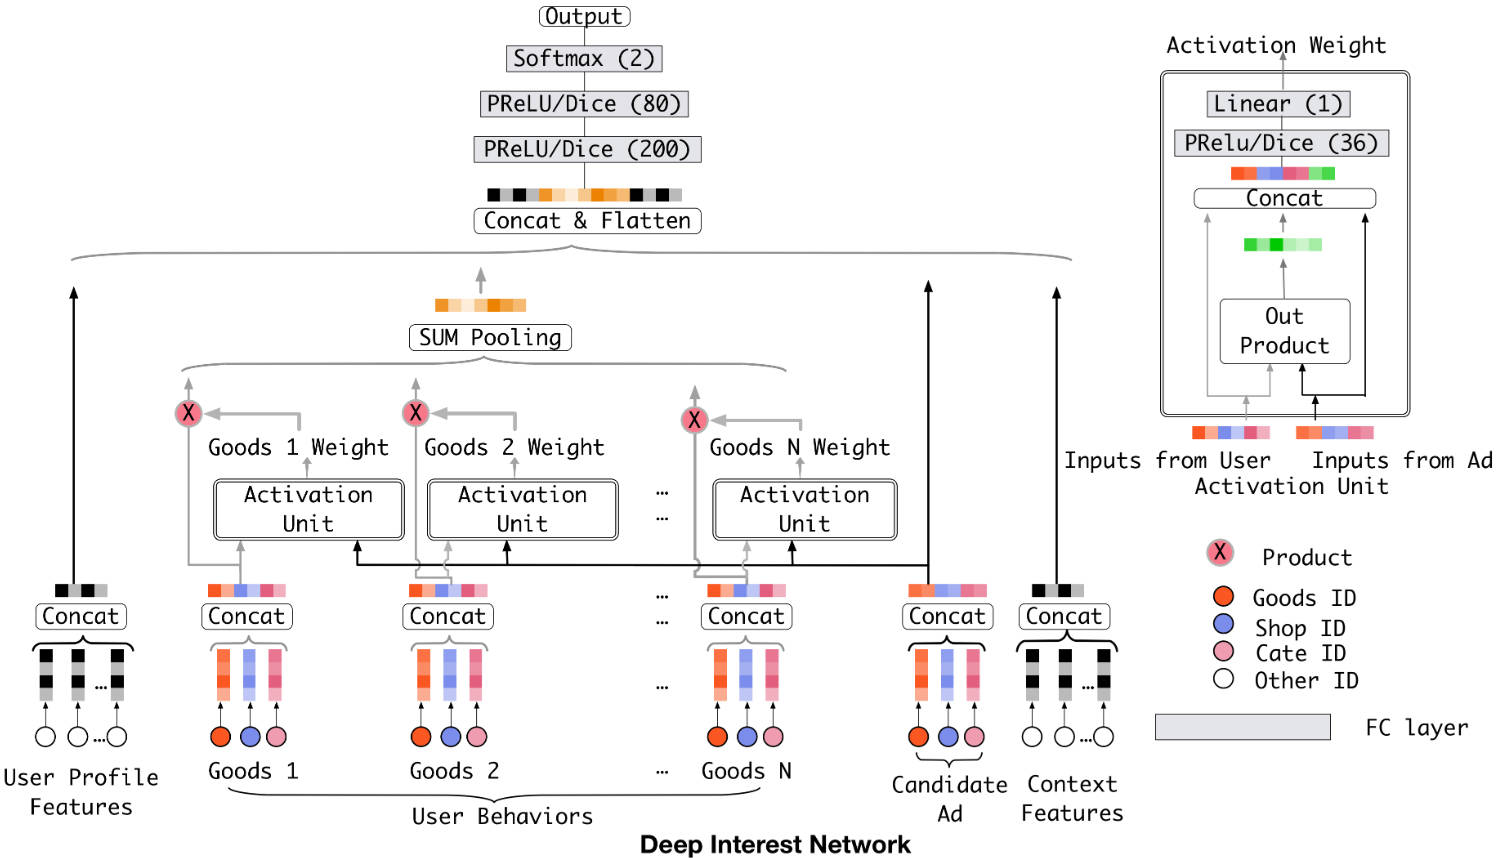
\includegraphics[width=\textwidth]{pics/din.jpg}
	\caption{Deep Interest Network}
	\label{fig:din}
\end{figure}

DIN 的主要创新体现在对用户多样化兴趣的建模上, 而这一步又是通过引入一个 Local Activation Unit 来做到的. 当然, 除此之外工程上的技术: mini-batch aware regularization、data adaptive activation function、GAUC. 其中关于用户兴趣的就是 Local Activation Unit. 

对于一个用户来说, 我们可以拿到 Ta 的行为序列, 在向其推荐物品时, 我们会有一个目标物品, 怎么利用行为序列来帮助预测呢?DIN 中利用目标物品与行为序列中物品的相关性来对用户兴趣进行建模, 即针对一个目标物品, 用户的表征/兴趣向量是其行为序列的加权求和, 权为行为序列与目标物品的相关性. 因此, 向同一个用户推荐不同的物品时, 其表征是不一样的. 相关性的计算就是通过 Local Activation Unit(LAU) 来计算的. LAU 的输入是行为序列中的物品的表征、目标物品的表征及二者的差 (论文中是 Product, 其实我感觉不重要, 只不过是前面两个的一个显式操作而已) , 三者拼接后进入前馈神经网络, 最后输出一个权重. 注意: \textbf{DIN 中并没有对这些权重进行归一化}, 论文中给出的原因是: 归一化后会弱化兴趣的强度. 

\textbf{为什么 DIN 中没有用 LSTM 来建模历史行为呢?} 论文中给出的答案是: 进行了尝试但是没有提升, 原因可能是用户行为序列与文本的不同. 文本序列是受语法约束的, 而用户的行为序列则不然, 可能同时包含多个兴趣, 可能在多个兴趣之间跳转. 

\subsubsection{不足}
\begin{myitemize}
	\item 没有考虑行为序列的序列信息, 即没有考虑物品的先后顺序. 这种情况下得到用户兴趣向量不能体现出用户的行为趋势, 而是基于整个序列进行推荐, 不是针对“下一次购买”进行推荐; 
	
	\item 只要推荐的物品与行为序列中的物品相似就会产生相似的用户向量, 即如果候选物品集都与行为序列有较高的相关性怎么办?这样产生的用户向量质量还好吗?
\end{myitemize}

\subsection{DIEN}
DIEN, Deep Interest Evolution Network, 诞生于阿里于 2019 年在 AAAI 上发表的论文 "Deep Interest Evolution Network for Click-Through Rate Prediction". 在 DIN 的基础上, DIEN 里考虑了用户兴趣的行为/兴趣的演化. 其结构如 Fig. \ref{fig:dien} 所示.

\subsubsection{Motivation}
对于 CTR 任务来说, 从用户行为背后捕捉用户的兴趣是十分关键的. 现有的一些用户兴趣建模中直接将用户行为的表示作为用户的兴趣, 而缺乏对行为背后的隐藏的兴趣的挖掘, 即行为不等价于兴趣. 并且因为外部环境和内部意识的改变, 用户的兴趣是动态的. 这些都是目前方法的不足.

\subsubsection{DIEN 怎么做的}
\begin{figure}[h]
	\centering
	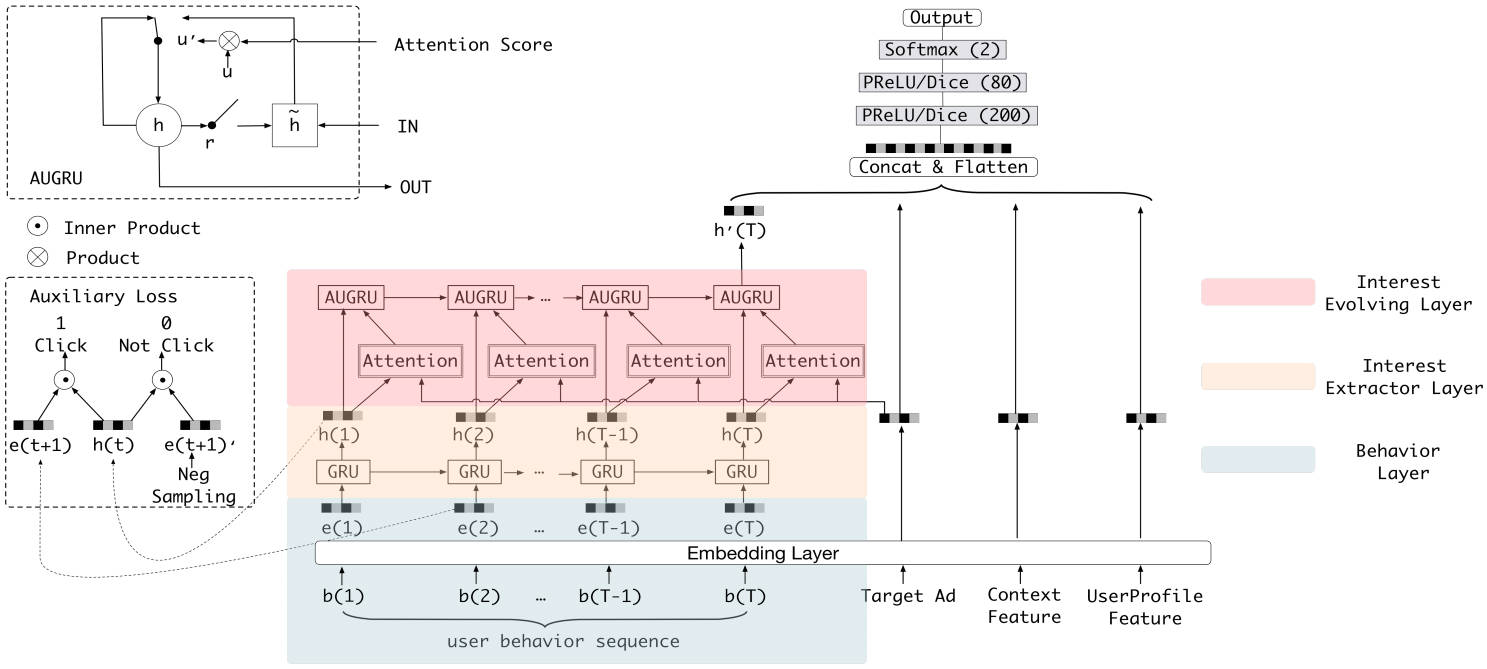
\includegraphics[width=\textwidth]{pics/dien.jpg}
	\caption{The structure of DIEN}
	\label{fig:dien}
\end{figure}

先介绍一个词, \textbf{Interest Drifting}, 兴趣漂移现象: 用户的意图在相邻的行为中可以有很大的差异, 一次行为的发生可能依赖的是很久之前的行为, 即之前的兴趣漂移到了现在, 不同的兴趣 (多峰兴趣) 有着各自的演化过程.

回顾一下 DIN: 通过嵌入层获得行为序列中每个行为的表征, 在通过局部激活单元进行 \textit{SUM Pooling}, 再与 \textit{target item} 及其他特征进行拼接, 最后输入到前馈网络中进行预测. 很明显, \textcolor{red}{DIN 直接将行为作为了用户的兴趣, 且没有考行为的序列特性}. DIEN 中通过两个模块来解决这些问题.

\paragraph{Interest Extractor Layer}
兴趣抽取层, 建模行为之间的依赖关系. DIEN 通过一个序列神经网络 (文中采用 GRU, 但就一般而言, 也可以采用其他网络, 如 LSTM, Transformer-Encoder 等) 来建模用户的连续行为, 并且引入了一个辅助损失来帮助学习来连续的行为. 这一部分的重点也就是辅助损失, 因此来看看辅助损失是怎么做的. 对于序列中的每个行为, GRU 都会输出一个 \textit{hidden state}, DIEN 中称之为 \textit{interest state}. 辅助损失将当前的行为当做 \textit{anchor}, 下一个行为作为 \textit{positive}, 随机采样一个样本作为 \textit{negative}, \textit{anchor, positive} 组成正样本, \textit{anchor, negative} 组成负样本, 以每个 \textit{anchor} 的正负样本构建损失:
$$
\begin{aligned}
	L_{a u x}=-& \frac{1}{N}\left(\sum_{i=1}^{N} \sum_{t} \log \sigma\left(\mathbf{h}_{t}^{i}, \mathbf{e}_{b}^{i}[t+1]\right)\right.\\
	&\left.+\log \left(1-\sigma\left(\mathbf{h}_{t}^{i}, \hat{\mathbf{e}}_{b}^{i}[t+1]\right)\right)\right)
\end{aligned}
$$
其中 $\mathbf{h}_t, \mathbf{e}_b^i[t+1], \hat{\mathbf{e}}_b^i[t+1]$ 分别表示 \textit{anchor, positive, negative}, $\sigma(\mathbf{x}_1, \mathbf{x}_2) = \frac{1}{1 + e^{-\mathbf{x}_1 \cdot \mathbf{x}_2}}$. 显然, $L_{aux}$ 就是个交叉熵损失函数. 引入辅助损失的好处: 1) 使 $\mathbf{h}_t$ 表达能力更强; 2) 减轻了 GRU 反向传播时的梯度弥散的问题. 

这一步, DIEN 将行为序列转换成了 \textit{interest states}, 不单单是行为序列的一个简单的表征, \textit{interest state} 还融入了序列信息, 把用户的兴趣从行为背后抽取出来.


\paragraph{Interest Evolving Layer}
兴趣演化层, \textbf{针对 \textit{target item}} 建模用户兴趣的演化过程, 其物理意义就是: 观察用户对 \textit{target item} 的兴趣在行为序列中是如何演化的. 为什么要针对 \textit{target item} 呢? 针对不同的物品 (方向), 用户的兴趣是有不同的演化路径的, 而演化路径就藏在行为序列中. 兴趣演化层可以看作是注意力机制, 把 \textit{target item} 当作 query 来匹配 key, 这一部分和 DIN 中的局部激活单元的功能是一致的. 兴趣演化层可以看作是 \textit{attention} 华和 \textit{GRU} 的结合.

首先, 是用 \textit{target item} 的表征取与兴趣抽取层每一步的输出 $\mathbf{h}_t$ 计算注意力:
$$
a_{t}=\frac{\exp \left(\mathbf{h}_{t} W \mathbf{e}_{a}\right)}{\sum_{j=1}^{T} \exp \left(\mathbf{h}_{j} W \mathbf{e}_{a}\right)}
$$
其中 $\mathbf{e}_a$ 就是 \textit{target item} 的表征. 兴趣演化层的 GRU 的输入就是兴趣抽取层的输出, 当然还把上一步计算得到的注意力融合进去, 怎么做呢? DIEN 文中设计了三种方案, 这三种方案的大体思路就是把 $a_t$ 与 GRU 里的某个部分乘起来. DIEN 中最后采用的方案是把 $a_t$ 与 GRU 中的更新门相乘, 并取名叫 \textit{GRU with attention update gate}(AUGRU). 

至此, DIEN 的结构就介绍完了.

\subsubsection{不足}
\begin{myitemize}
	\item GRU 的计算只能是串行的, 计算的时间复杂度是较高的, 在线上部署是会有较大的延迟;
\end{myitemize}


参考资料
\begin{myitemize}
	\item \href{https://mp.weixin.qq.com/s?__biz=MzU0MDA1MzI0Mw==&mid=2247488129&idx=1&sn=ed882611a06b75e8e819b519010e9e81&chksm=fb3e4915cc49c003cb4505d0b09f06fa1c4e92409270b49f5509f1902774234382ba05b400d8&scene=21#wechat_redirect}{浅谈行为序列建模};
	
	\item \href{https://mp.weixin.qq.com/s?__biz=MzI5NTU2ODQzMg==&mid=2247484150&idx=1&sn=3bdb017a542bc2e2b94404f46ec9eb4f&chksm=ec50d7a9db275ebfdc009e6be3ea6a0ee8209477dafc99bc8a6a212fa0456a14bf4453b826dd&scene=21#wechat_redirect}{刀工: 谈推荐系统特征工程中的几个高级技巧};
	
	\item \href{https://mp.weixin.qq.com/s/o04b8gN4TYecKHopXGMuVg}{日久见人心:论建模用户长期兴趣的几种姿势}
\end{myitemize}

\section{多任务学习}
\subsection{Introduction}
在搜索或推荐领域, 准确率通常是我们想到的第一个目标, 但真的是这样吗? 说到底, 各个平台的最终目的是为提供令用户更满意的服务, 为平台留住用户, 创造更多的利益. 为达成这些目的, 准确率够吗?

就视频推荐而言, 以单个目标作为优化对象的问题:
\begin{myitemize}
	\item 目标偏差: 点赞, 分享表达的满意度比播放更高;
	
	\item 物品偏差: 不同视频的播放时长体现的满意度不一致;
	
	\item 用户偏差: 有的用户偏向于点赞, 而有的偏向于收藏.
\end{myitemize}

选择哪个目标来进行优化才能满足我们的要求呢? 一个比较直接的方式就是同时优化所有的目标: 1) 单目标难以直接衡量用户满意度, 多目标优化可以最大限度地利用丰富的隐式反馈数据建模用户满意度; 2) 推荐系统排序模块要求低时延, 多目标优化训练一个模型可以预测多个目标, 线上融合多目标的预测结果进行排序.


多目标任务的常用模型: 
\begin{myitemize}
	\item Shared-Bottom;
	\item One-gate MOE(Mixture-of-Experts);
	\item ESMM, SIGIR'2018;
	\item MMoE, KDD'2018;
	
	\item SNR(Subnetwork Routing), AAAI'2019;
	\item PLE, RecSys'2020;
\end{myitemize}

多任务学习通常通过 Hard 或 Soft 参数共享来完成: 
\begin{myitemize}
	\item 共享 Hard 参数是神经网络 MTL 最常用的方法, 可以追溯 1993 年 Caruana 所发表的论文. 在实际应用中, 通常通过在所有任务之间共享隐藏层, 同时保留几个特定任务的输出层来实现. 共享Hard 参数大大降低了过拟合的风险. 1997 年 Jonathan Baxter 在他的论文中证明过拟合共享参数的风险为 O(N)——其中 N 是任务数——小于过拟合特定任务参数, 即输出层. 这很直观: \textbf{同时学习的任务越多, 模型找到一个含有所有任务的表征就越困难, 而过拟合原始任务的可能性就越小};
	
	\item 另一方面, 在共享 Soft 参数时, 每个任务都有自己的参数和模型. 模型参数之间的距离是正则化的, 以便鼓励参数相似化. 1998 年 Caruana 对早期的 MTL 的研究进行了总结, 并演示了三个领域中的多任务学习. 他们解释了多任务学习的工作原理, 提出了一个基于案例的方法 (如 kNN 和核回归) 的多任务学习算法和结果, 并为决策树中的多任务学习绘制了一个算法. 目前大部分MTL学习所基于的机制仍然来源于此篇文章.
\end{myitemize}
 

MTL 通常受到数据分布以及任务之间相关性的影响 (\textbf{如何衡量任务之间的相关性、关系}) . 

\subsection{多目标任务的技巧}
\subsubsection{样本加权}
在优化主目标的同时, 将其他目标转化为样本权重, 借此来达到优化其他目标的效果. 例如主目标为 CTR, 同时还有一个目标是停留时长. 则可以给停留时长长的样本赋予更高的权重. 

\textbf{特点}: 这种方式模型简单, 上线容易, 仅在训练时通过梯度乘以权重实现对其他目标的加权即可. 但本质上不是多目标建模, 而是将多个目标转化为一个目标, 目标的加权权重需要根据线上 A/B 测试才能确定. 而且, 可能不适用于多个从目标的情况, 因为将多个从目标转化为样本权重很难找到一个合适的平衡. 

\subsubsection{模型融合}
多目标模型融合, 通过将一个模型同时训练多个目标 (label 的构造) . 该方法的优点是各个任务之间能够共享信息, 同意迭代方便, 节省资源. 缺点: 目标越多模型越复杂, 各个任务之间相互影响, 迭代速度慢. 


\subsection{ESMM}
ESSM, Entire Space Multi-task Model, 诞生于阿里于 2018 年在 SIGIR 上发表的论文 "Entire Space Multi-Task Model: An Efficient Approach for Estimating Post-Click Conversion Rate". 该论文针对 CVR 估计中的样本选择偏差 (Sample Selection Bias, SSB) 和 数据稀疏 (Data Sparsity, DS) 问题, 提出了一个多任务学习的模型, 模型结构如 Fig.\ref{fig:esmm} 所示.

\begin{figure}[h]
	\centering
	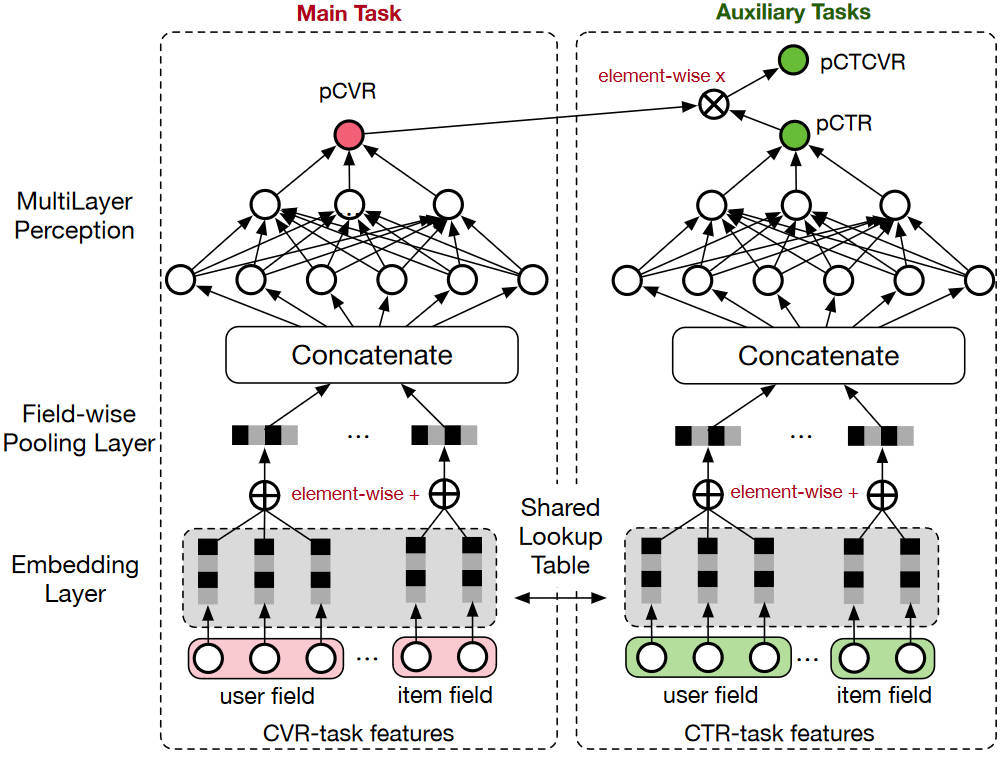
\includegraphics[width=\textwidth]{pics/esmm.jpg}
	\caption{The structure of ESMM}
	\label{fig:esmm}
\end{figure}

\subsubsection{Motivation}
转化率预估(CVR)目前主要存在两个难点: 
\begin{itemize}
	\item SSB. 从 CVR 模型使用的角度来看, 其训练过程是\textcolor{red}{有偏}的. CVR 预估模型是\textbf{在点击的样本上进行训练的}, 但是被用于\textcolor{red}{在整个样本空间上进行推断}. 这样做实际上存在一个问题, 训练和预测的数据分布的不一致会损害模型的泛化能力;
	
	\item DS. 实际上CTR预估的数据就已经非常稀疏了, 点击后再转化的数据则更少了;
\end{itemize}

ESMM(Entire Space Multi-Task Model) 并没有直接在整个样本空间上去预估CVR, 而是采用两个辅助的任务: CTR 和 CTCVR 来间接的预测 CVR, 而不是直接通过在点击数据上训练 CVR 模型, 因为这些数据是有偏的, 如果直接用其余样本作为负样本, \textbf{并不知道这些没被转化是因为没被点击还是因为其他原因}.

\subsubsection{HOW}
\begin{figure}[h]
	\centering
	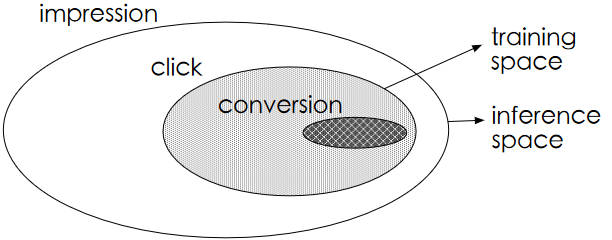
\includegraphics[width=.5\textwidth]{pics/ssb.jpg}
	\caption{Illustration of sample selection bias problem in conventional CVR modeling. Training space is composed of samples with clicked impressions. It is only part of the inference space which is composed of all impressions.}
	\label{fig:ssb}
\end{figure}

结合 Fig.\ref{fig:esmm} 来看, \textit{Main Task} 是 pCVR, 两个辅助任务是 pCTR, pCTCVR, 被估计的样本是 $x$. 先看看各个任务的\textbf{训练样本}是什么:
\begin{itemize}
	\item pCTR: 曝光样本空间, 即 Fig.\ref{fig:ssb} 中的 impression, 曝光中点击的 ($y=1$) 作为正样本, 未点击的作为负样本;
	
	\item pCVR: 点击空间, 即 Fig.\ref{fig:ssb} 中的click, 转化的 ($z=1$) 作为正样本, 未转化的作为负样本;
	
	\item pCTCVR: 曝光空间, 点击且转化的 ($y=1\&z=1$) 作为正样本;
\end{itemize}
要注意: \textbf{\textcolor{red}{pCVR 是在整个曝光空间上推断时}} --- SSB 问题的来源. 那能不能在整个曝光空间上来训练 pCVR 呢? 回顾一下 ESMM 的名字 "\textbf{Entire Space} Multi-Task Model", 重点在于这个 Entire Space, 这个空间指的就是 Fig.\ref{fig:ssb} 中的 impression. 其实这也回答了刚刚的问题, 可以在整个曝光空间上训练 pCVR. 那就来看看 ESMM 怎么做的.

ESMM 中并不直接去估计 pCVR, 而是去估计 pCTR 和 pCTCVR. 这两个辅助任务的训练空间都是曝光空间. 这两个辅助任务与主任务之间的关系:
$$
\underbrace{p(y=1, z=1 \mid x)}_{p C T C V R}=\underbrace{p(y=1 \mid x)}_{p C T R} \times \underbrace{p(z=1 \mid y=1, x)}_{p C V R}
$$

如 Fig.\ref{fig:esmm} 所示, ESMM 由两个子网络组成, 左边的估计 pCVR, 右边的估计 pCTR, 二者相乘得到 pCTCVR, 实际训练时只针对 pCTR 和 pCTCVR 计算损失:
$$
\begin{aligned}
	L\left(\theta_{c v r}, \theta_{c t r}\right) &=\sum_{i=1}^{N} l\left(y_{i}, f\left(x_{i} ; \theta_{c t r}\right)\right) \\
	&+\sum_{i=1}^{N} l\left(y_{i} \& z_{i}, f\left(x_{i} ; \theta_{c t r}\right) \times f\left(x_{i} ; \theta_{c v r}\right)\right)
\end{aligned}
$$
ESMM 的目的是训练一个能够在全样本空间上进行 CVR 估计的模型, 但是并没有直接去训练这个模型的参数, 而是通过 pCTR, pCTCVR 与 pCVR 之间的约束关系 $pCTCVR = pCTR * pCVR$ 来学习 pCVR 模型的参数. 其实, 也可以分别单独估计 pCTR 和 pCTCVR 再来求 pCVR, 但是这样会有两个问题: 1) CTR, CTCVR 都是很小的数, 做除法会有数值上的不稳定, 而且 2)单独估计时二者之间不存在约束关系, 做除法时可能会得到大于 1 的 CVR.

\subsubsection{总结}
\begin{itemize}
	\item ESMM 通过多任务学习来解决 CVR 样本空间在训练和推理时不一致的问题, 利用了 CVR, CTR 这两个目标之间的依赖关系;
	
	\item ESMM 这种形式可以推广到目标\textbf{具有依赖关系}的场景中, \textcolor{red}{对于关系比较模糊的场景该怎么办呢?}
	
	\item 真实场景中, 可以直接使用 CVR 的模型来进行打分作为排序的依据;
\end{itemize}

\subsection{Shared-Bottom}
简称为 SB, 即多个任务之间有一个共享的底座. SB 是由 Rich Caruana 与 1997 年在其博士论文中提出来的. SB 有一个被多个任务共享的模块 (shared-bottom network), 该模块的输出作为各个任务的输入, 每个任务有一个单独的网络来学习.

\subsection{MMoE}
MMoE, Multi-gate Mixture-of-Experts, 诞生于 Google 于 2018 年八月在 KDD 上发表的论文 "Modeling Task Relationships in Multi-task Learning with Multi-gate Mixture-of-Experts". 基于 NN 的多任务学习模型一般对任务之间的关系比较敏感, 即在相关性强的任务上效果好, 相关性弱的效果差. 该论文提出了 MMoE 来克服任务间关系敏感的问题.

\subsubsection{Motivation}
在很多场景中, 通常是要同时考虑多个目标的, 一开始大家都是未每个任务建一个模型, 但是随着数据量和业务规模的扩大和复杂化, 一个任务一个模型的成本越来越高, 效果也不太稳定. 那么能不能同时对所有任务一起建模, 一起学习和优化呢? 当然是可以的, 这方面的尝试也早就开始了 --- multi-task learning. 但有时多任务学习的效果并不如单个模型独立学习, 这里面是有很多原因造成的, 例如任务之间的相关性, 差异性. 其中一个主要的原因就是\textcolor{red}{\textbf{任务间的关系 / 差异}}, 这也是大家研究的较多的一个方向. 为什么任务间差异大效果就不好呢? 由于任务间差异大, 可能各个任务的最优解是相距很远的, 甚至是互斥的. 以往的工作为了弥补任务间的差异, 会引入更多的参数, 这样做会增加学习的计算量, 而且在真实的场景中有些参数是不可获得的.

\subsubsection{HOW}

\begin{figure}[h]
	\centering
	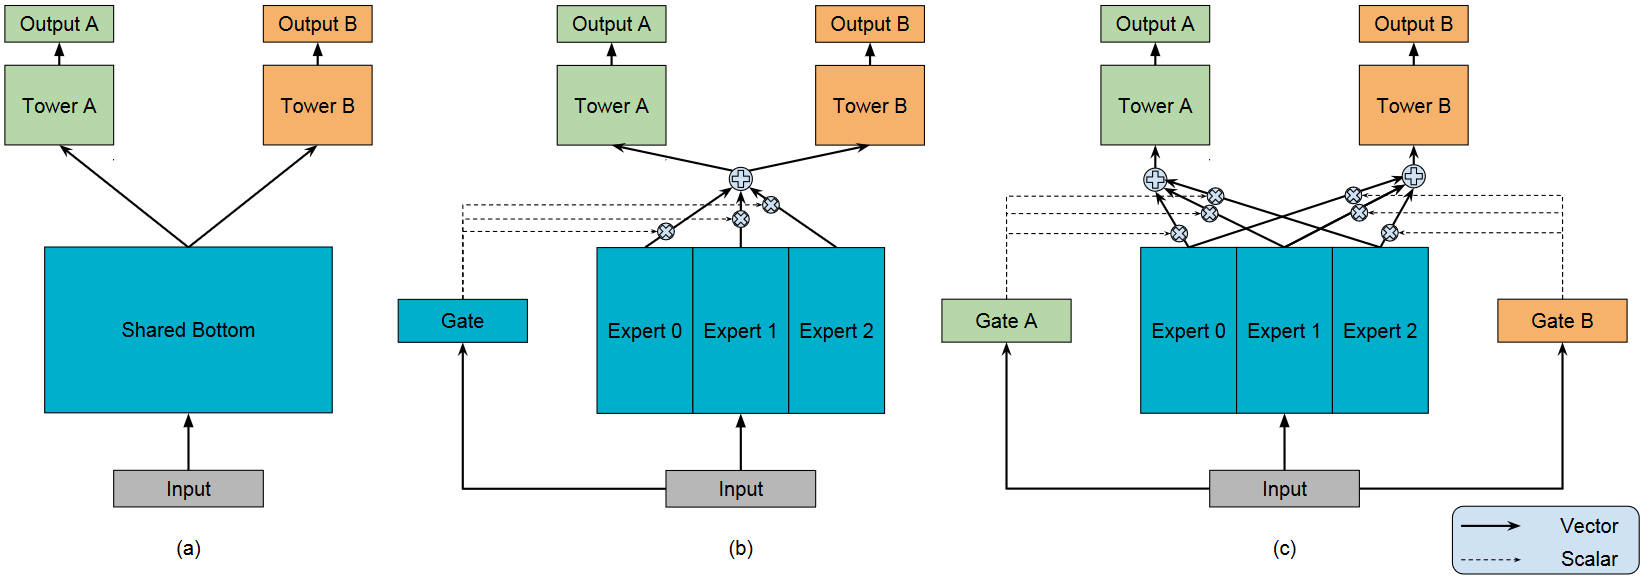
\includegraphics[width=.85\textwidth]{pics/mmoe.jpg}
	\caption{(a) Shared-Bottom model. (b) One-gate MoE model. (c) Multi-gate MoE model.}
	\label{fig:mmoe}
\end{figure}

MMoE 的模型结构如 Fig. \ref{fig:mmoe} (c) 所示. 可以看到, 这三个模型是有明显的递进关系的, 从 SB 的单个 shared-bottom 到 MoE 的多个 shared-bottom, 从 MoE 的单门控到 MMoE 的多门控. 



\clearpage
\part{Information Retrieval}
{\noindent}	 \rule[-10pt]{17.5cm}{0.5em}\\
\section{Basic}
\subsection{术语}
\paragraph{qanchor}
Qanchor 是针对 doc 而言的, 把 query 当作 doc 的 qanchor. 例如在点击图中, 与一个 doc 相连的多个 query, 那么则可以把这些 query 当作 doc 的 qanchor.
\section{Learning to Rank}
\subsection{排序学习算法简介}
排序学习, Learning to Rank, 简言之: 给定一个查询$q$, 和待查询的数据集合$D$, 返回与$q$最相关的top k(有序)的结果或者给出$D$中所有元素与$q$的相关性排序. 

\subsubsection{Pointwise}
将排序问题转化为分类、回归问题. 以一个$q$和一个待查询对象$q$(只有一个待查询对象, 这也是Point的原因)之间的相关性作为预测目标, 即$Pointwise: q \times d \rightarrow label, q \in Q, d \in D$, 以$(q, d)$作为训练样本. 

Pointwise缺点: 
\begin{itemize}
	\item 只考虑了某个查询下, 单个待查询对象的相关性, 没有考虑该查询下所有待查询对象的排序关系, 即带查询对象间的关系
	\item 查询时, 往往排在前面的对象比后面的对象更重要, 而Pointwise平等地对待所有带查询对象, 损失函数会被占多数的非top K对象所影响
\end{itemize}


\subsubsection{Pairwise}
针对一个查询$q$, 通过某种方法确定一个大致的待查询对象集合$D_q$, Pairwise将排序问题转化为$D_q$中任意两个对象之间相对关系的分类/回归问题, 训练样本为$(d_i, d_j),\: d_i, d_j \in D_q$, 预测目标为$d_i, d_j$与$q$的相关性的相对大小, 例如1表示$q_i$比$q_j$更相关. 

Pairwise缺点: 
\begin{itemize}
	\item 是在两个带查询对象之间的相关性的基础上学习的, 学习的它们的相对顺序, 并不是文档在最终的结果列表中的顺序
	\item 不同的查询可能会有不同大小的带查询对象集合, 这种不均衡问题会影响算法的评估与学习
\end{itemize}


\subsubsection{Listwise}
Listwise将一个query对应的所有相关待查询对象看作一个整体, 作为单个训练样本, 直接优化MAP、NDCG(Normalized Discounted Cumulative Gain)这样的指标, 从而学习到最佳排序结果. 


\subsection{LambdaMart}



\clearpage
\part{Algorithms}
{\noindent}	 \rule[-10pt]{17.5cm}{0.5em}\\
\section{Basic}
\subsection{大整数}
\paragraph{Motivation}在C、C++等一些语言中,支持的整数类型所能保存的范围是有效的,相对Java、Python等一些语言中支持的范围是要小的。

\paragraph{HOW?}考虑几个可能的涉及大整数的例子:大整数的加法、大整数的减法大整数乘某个数大整数除以某个数。主要涉及到的问题有:
\begin{itemize}
	\item 大整数的存储
	\item 大整数之间的加减法
	\item 大整数与一个常规整数的乘除法
\end{itemize}


\subsection{前缀和与差分}


\subsection{并查集}
\paragraph{Motivation}将n个不同的元素分成一组\textbf{不相交}的集合。能够快速地完成两种操作:查找某个元素属于那个集合、合并两个集合。注意:“不相交”可以有不同的定义,如graph中的节点是否相邻、在某种度量下的不相交等。

\paragraph{HOW?}
\section{Search}
\subsubsection{贪心算法}
贪心搜索是一种搜索解空间的策略,在搜索时,基于当前状态,选择代价最低或估计收益最大的方向作为下一步搜索的方向。使用贪心搜索并不能保证全局最优解,目的是为了找到一个可行解。在使用贪心算法前,先要证明以下两个东西:
\begin{itemize}
	\item 贪心选择性:指所求问题的整体最优解可以通过一系列局部最优的选择(通过最优度量标准来判断)来到达
	\item 最优子结构:一个问题的最优解中包含了子问题(比原问题规模更小的问题)的最优解,即每一步贪心选完后会留下子问题,子问题的最优解和贪心选出来的解可以凑成原问题的最优解
\end{itemize}
和动态规划相比,二者都需要描述清除问题的优化子结构;但是贪心算法重点是证明贪心选择的合理性,DP重点是找到子问题和合理的递推关系式。

典型的贪心问题:Huffman编码、活动选择问题。



\subsubsection{Beam Search}
也叫集束搜索。
对贪心搜索的一种改进。在进行搜索时,并不是只沿一个方向搜索,会同时保留$n$个最优的方向,分别以这$n$个方向进行扩展,扩展后在每个方向都可以得到$n$个备选项,那么则有$n^2$个备选项,在这$n^2$个被选项里选择最优的$n$个备选项作为下次扩展的方向,以此类推,即在搜索树的每一层都只保留$n$个方向。$n$就是beam width。





\clearpage
\part{Coding Practice}
{\noindent}	 \rule[-10pt]{17.5cm}{0.5em}\\

\section{C++}
参考文档: \href{https://www.cplusplus.com/}{cplusplus.com}
\subsection{C++数据类型转换}
\paragraph{数字 <=> 字符串}
\begin{itemize}
	\item itoa: 整数转为字符串, 可以设置基底
	\item stoi: 字符串转为整数 , 可以设置基底
	\item atoi、atol、atoll: 将字符串转为int/long/long long, 可以设置基底
	\item to\_string: 可以讲数字转为字符串, 包括整数、小数等
\end{itemize}

\subsection{C++集合} 通过$\#include<set>$来引入set. 关于集合的一些运算, 包含在algorithm库中. 在algorithm库中有一个includes函数, 可以用来判断两个容器之间是否存在包含关系, 但是, 要注意\tbc{red}{两个容器都要先从小到大进行排序!!!}
\begin{cpp}
	// 省略头文件和库的包含代码
	int container[] = {5,10,15,20,25,30,35,45,50};
	int continent[] = {40,30,20,10};
	
	sort (container,container+10);
	sort (continent,continent+4);
	
	// using default comparison:
	if ( std::includes(container,container+10,continent,continent+3) )
		cout << "container includes continent!\n";
	else	cout<<"NO\n";
	
\end{cpp}


\subsection{字符串}
C++中字符串用双引号括起来, 字符用单引号括起来. 
\paragraph{字符串比较}
compare

\paragraph{常用方法}
\begin{itemize}
	\item 初始化: \mintinline{cpp}{string s(n, 'c');}
	\item 插入字符串: \mintinline{cpp}{s.insert(pos, len, "insert");}
	\item 删除子串: \mintinline{cpp}{s.erase(pos, len, "erase");}
	\item 
\end{itemize}

\subsection{数组}
\paragraph{数组初始化}
\begin{itemize}
	\item \mintinline{cpp}{type [][depth][depth]...[depth]}声明多维数组时, 只能有一维的大小不指定
	\item \mintinline{cpp}{int arr[5] = {1, 2, 3, 4, 5}}声明数组时可以给数组赋值(初始化列表), 如果指定的数组大小则$\{\}$中的值的数量应该小于等于数组大小, 如果数量小于数组大小, 则数组中后续位置将会被填充默认值(对于基础类型, 则为0). 因此, 当$\{\}$未空时, 数组将会被填充为默认值
	\item \mintinline{cpp}{int *p = new int[5]}将在堆中分配内存, 此时也可以对数组进行初始化: \mintinline{cpp}{int *p = new int[]{1, 2, 3, 4, 5}}、\mintinline{cpp}{int *p = new int[]()}. 对于基本类型, 如果不进行初始化, 局部定义的数组的值是未定义的;对于类类型, 会默认调用其默认构造函数. \textbf{堆中分配的数组要用delete删除}
\end{itemize}

\subsection{遍历vector的方式}
\begin{cpp}
	vector<int> nums = {1, 2, 3, 4, 5};
	// 方法1: 下标
	for(int i = 0; i < nums.size(); i++){
		// do something
	}
	
	// 方法2: 迭代器
	for(vector<int>::iterator it = nums.begin(); it != nums.end(); it++){
		// do something
	}

	// 方法3: auto, 以引用的形式遍历, 可以修改值
	for(auto &it: nums){
		// do something 
	}

	// 方法4: auto, 以值的形式遍历, 不可以修改值
	for(auto it: nums){
		// do something
	}
	
	// 方法5: for_each
	foreach(nums.begin(), nums.end(),
			[](const auto &val) -> void { 
				// do something
			})
	
\end{cpp}

\subsection{for\_each}
for\_each源码如下: 
\begin{cpp}
	template<class InputIterator, class Function>
	Function for_each(InputIterator first, InputIterator last, Function fn)
	{
		while (first!=last) {
			fn (*first);
			++first;
		}
		return fn;      // or, since C++11: return move(fn);
	}
\end{cpp}
其中参数fn是一个一元函数(即只能有一个参数), 它的返回值会被忽略. 

\subsection{deque}
\mintinline{cpp}{#include <deque>}. double ended queue, 双端队列. \href{https://www.cplusplus.com/reference/deque/deque/?kw=deque}{dequ}e是一种动态容器(通常以动态数组的形式, 如链表, 来实现), 可以在两端增加或者删除元素, 随机访问deque中的元素. 

\subsection{priority\_queue}
\mintinline[bgcolor=yellow]{cpp}{#include <queue>}. 
\begin{minted}{cpp}
	template <class T, class Container = vector<T>,
	class Compare = less<typename Container::value_type> > class priority_queue;
\end{minted}
\href{https://www.cplusplus.com/reference/queue/priority_queue/?kw=priority_queue}{priority\_queue}, 优先队列. priority\_queue是一种容器适配器(container adaptor), 它使用某种容器(可以是queue、vector等, 默认是vector)作为其数据的容器, 并提供了一些接口来访问容器内的元素, 重点就在这些接口上(\mintinline{cpp}{push, pop, top})!priority\_queue的特点: 
\begin{myitemize}
	\item 第一个元素是优先级最大/小的元素(大/小根堆)
	\item \mintinline{cpp}{top} : 返回顶部的元素, 即优先级最大/最小的元素
	\item \mintinline{cpp}{pop} : 删除顶部的元素
\end{myitemize}
例子: 
\begin{minted}[linenos, breakafter=true,autogobble=true,frame=leftline]{cpp}
	#incldue <queue>
	
	int main(){
		// 大根堆
		priority_queue<int> a; // <=> priority_queue<int, vector<int>, less<int> >a
		
		// 小根堆
		priority_queue<int, vector<int>, greater<int> > b;
	}
\end{minted}




\section{Python}
\subsection{basics}
\subsubsection{defaultdict} python中的defaultdict,也是一种dict。与传统的dict不同,当传统的dict的key不存在时会Error,但defaultdict不会,而是返回一个默认值。该默认值由创建defaultdict时传入的参数有关:$dd = defaultdict(default_factory)$。

当default\_factory是list时,默认值是[],defaultdict其他常见取值还有:str, set, int, dict。但不可以是defaultdict。

\subsubsection{glob} python中的一个内置模块,用于查找符合特定规则的文件路劲。如:
\begin{python}
	import glob
	pattern = "./myfloder/prefix-*.txt"
	li = glob.glob(pattern) # 此时li中就包含了所有符合pattern这个模式的文件名
\end{python}

\subsubsection{python format用法}
\textbf{对齐}"$\{:\}$" 通常将对齐符号放在$:$后。\^ 、| < | >分别是居中、左对齐、右对齐,在填充符号后面可带宽度,在$:$后可带填充字符,默认为空格。

\subsubsection{数字输出格式}主要包括小数位数(如.2f)、百分号输出(如.2\%)、指数形式输出(如.2e)、带正负符号的输出(如+.2f)、按不同进制的输出(b、d、o、x分别是二进制、十进制、八进制、十六进制,在b|o|x前加\#可以输出进制符号,x的大小写会影响进制符号的大小写。
\begin{python}
	"{:^8}".format("居中")	# 居中显示,宽度为8,默认用空格填充
	"{:*<8}".format("左对齐")	# 左对齐显示,宽度为8,用*填充
	"{:*>8}".format("右对齐")	# 右对齐显示,宽度为8,默认用空格填充
	"{:.2f}".format(123)
	"{:.2%}".format(123)
		"{:^8.2f}".format(123)		# 八位的显示宽度,保留2位小数
		"{:b}".format(11)
		"{:d}".format(11)
		"{:o}".format(11)
		"{:x}".format(11)
		"{:#x}".format(11)
		"{:#X}".format(11)
	\end{python}


\subsection{numpy}
\subsubsection{np.argsort} 对数组的元素进行排序(默认是从小到大),生成一个新的数组,数组元素是排序后的数组所对应的下标。
\begin{python}
	import numpy as np
	x = np.array([2,1,3,5,4])
	y = np.argsort(x) # y = [1, 0, 2, 4, 3]
	# 从大到小排序
	y = np.argsort(-x) # y = [3, 4, 2, 0, 1]
\end{python}
该方法还有更复杂的使用方法,可以根据参数进行调节,$argsort(a, axis=-1, kind=None, order=None)$。

\subsubsection{numpy设置随机数种子} $np.random.seed(seed)$。





\subsubsection{numpy nan的处理}numpy中可以使用np.isnan()来判断数组中的元素是否为NAN,返回的结果与数组形状相同,元素为True/False,该位置的元素为NAN是则为True,否则为False。可以使用 np.nan\_to\_num(x, copy=True, nan=0, posinf= 1.7976931348623157e+308, neginf=-1.7976931348623157e+308) 来进行转换。该函数可以将NAN(包括无穷小、无穷大)转换为数字,可以指定转换后的数字。参数:x是待转换的数据,可以是数组或单个数字;copy表示是否进行原地转换,相当于pandas中的in\_place参数,但取值与in\_place相反;nan表示取代NAN的数字;posinf、neginf表示用什么取代正/负无穷。

\subsubsection{找到数组中nan指的位置}:np.argwhere(np.isnan(a))。解释:通过np.isnan标记数组中nan值的位置为True,np.argwhere会返回那些True的下标。


\subsection{matplotlib}
\subsubsection{matplotlib中的marker}如图\ref{fig:matplotlib-markers}所示,更多内容可参见:\href{https://matplotlib.org/api/_as_gen/matplotlib.pyplot.plot.html#matplotlib.pyplot.plot}{Matplotlib}
\begin{figure}[h]
	\centering
	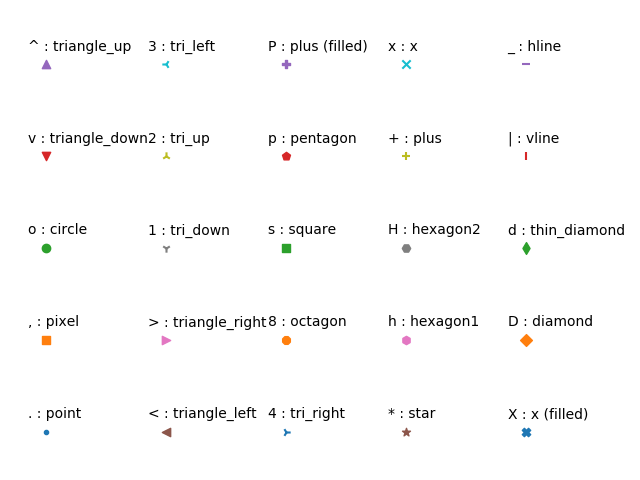
\includegraphics[width=.65\textwidth]{pics/markers.png}
	\caption{Matplotlib中的markers}
	\label{fig:matplotlib-markers}
\end{figure}

\subsubsection{Animation}
Animation可用于制作动画。初始化函数:
\begin{python}
	def __init__(self, fig, func, frames=None, init_func=None, fargs=None,
	save_count=None, *, cache_frame_data=True, **kwargs)
	"""
	fig: 绘制动画的地方
	func: 完成动画动作的回调函数。定义应为:def func(frame, *fargs) -> iterable_of_artists
	frames: 可以认为是每一个动画帧的索引,通常为iterable对象,frames中的每个值会逐个作为func的第一个参数传入
	init_func: 在绘制第一帧之前调用的函数,定义应为:def init_func() -> iterable_of_artists
	fargs: 用于func的额外的参数
	repeat_delay: 帧之间的延迟,单位为毫秒
	repeat: 是否重复播放动画
	blit: 布尔值故, 默认为False。用于优化绘图,注意这个参数有点坑,当其为True时,会根据artists的zorder来绘图,当对象没有zorder(如bar)时则会报错
	"""
\end{python}
在使用matplotlib制作动画的过程中,很重要的是要知道要让什么对象发生变化、发生什么变化 --- 知道了这二者之后就可以在每一帧的更新函数中完成对应的动作了。

\tbc{red}{注意}:blit参数的使用,当启用了blit时,且要对bar改变时,则会报错:\textit{AttributeError: 'BarContainer' object has no attribute 'get\_zorder'},把blit设为False即可。


\subsubsection{调整子图间距}
\begin{itemize}
	\item plt.tight\_layout()
	\item plt.subplot\_adjust(left=None, bottom=None, right=None, top=None, wspace=None, hspace=None)
\end{itemize}

\subsubsection{显示中文}
\begin{python}
	plt.rcParams['font.sans-serif'] = ['SimHei'] # 步骤一(替换sans-serif字体)  
	plt.rcParams['axes.unicode_minus'] = False  # 步骤二(解决坐标轴负数的负号显示问题)
\end{python}

\subsection{python中的线程有什么问题?怎么解决?}
python 中有一个叫 GIL(Global Interpreter Lock,全局解释器锁) 的玩意儿,每个线程想要执行必须先获取到这把锁,不管你 CPU 有几个核心,锁只有一把。所以每次只能有一个线程在执行。

\subsection{有序数组中找到一个数字的插入位置}
 





\section{Tensorflow}
\subsection{tf.variable\_scope \& tf.name\_scope}

\subsection{tf.sparse\_tensor}	tf中的稀疏张量。使用三个稠密的张量来表示。
\begin{itemize}
	\item indices: 表示原张量中非零值的位置
	\item values: 表示indices中元素所指位置上的值
	\item dense\_shape: 表示原张量的shape
\end{itemize}

\subsection{tf.train.Saver}tf中用于保存、恢复模型参数的接口。主要由两个接口:1)tf.train.Saver().save()用于保存模型;2)tf.train.Saver().restore()用于回复模型。
\begin{python}
	import tensorflow as tf
	saver = tf.train.Saver(max\_to\_keep=3) # max\_to\_keep表示保存的checkpoint最大次数
	...
	# 保存模型
	# sess: 会话的名字
	# save\_path: 模型的保存路径
	# global\_step: 保存模型时的后缀
	# 使用以下方法保存模型后会产生四个文件,分别是:
	# checkpoint文件:会记录最新的模型是哪个
	# .ckpt.meta文件:包含元图,保存了计算图的结构,没有变量的值
	# .ckpt.data 文件:保存权重等参数
	# .ckpt.index 文件:为数据文件提供索引,{还不太确定}
	saver.save(sess=sess, save_path=model_save_path, global_step=step)
	...
	# 恢复模型
	# save_path可以不用加模型的后缀
	saver.restore(sess=sess, save_path=model_save_path)
\end{python}

\subsection{tf.Session}运行tf中操作的类,Session类封装了运行操作所需要的环境。可以使用手动开启和关闭、上下文的方式使用Session。在使用Session时还可以进行配置,将配置作为Session初始化的参数传入。

\subsection{tf中的RNN}RNN的训练数据与其他神经网络的训练数据有一点不一样。通常的NN中的训练数据,每个样本就是一个向量。但是在RNN中,每个训练样本就是一个矩阵,每一行表示一步的输入,正因为RNN所处理的问题不同,RNN的输出数据也变得更加复杂。\\
针对不同的RNN有不同形式的输出,但可以进行简单的归纳:对于RNN中的每个样本,其形式为$\mathbb{R}^{max\_time \times embed\_size}$,其中$max\_time$表示所有样本中序列的最大长度,$embed\_size$表示每一步的输入的长度。当输入了一个样本后,会将样本的每一行 --- 即每一步的数据输入到RNN中,由于RNN本身的特点,每一步都可以产生输出,通常来说包含每一步的输出和状态(具体到不同的RNN时会有不同)。每一步的输出维度会收到RNN模型隐层宽度 --- 即隐层单元数量的影响。并且针对不同的任务,最终需要的输出是不一样,例如m对n、m对1、m对m的任务等等。\\
在tf中,有多种关于RNN单元的类,如BasicLSTMCell、GRUCell、MultiRNNCell。可以在这些类的基础上搭建自己的RNN模型。


\subsection{ImageDataGenerator}
这是Keras中的一个图像数据生成器,同时也可以在batch中对数据进行增强,扩充数据集大小,增强模型的泛化能力。比如进行旋转,变形,归一化等。

\subsection{tf.where}
tf.where(condition, x=None, y=None, name=None)

condition是一个布尔数组,condition、x、y的维度必须相同。

其中x、y可以为None,此时返回的是一个二维数组,该二维数组的行数表示condition中为True的元素的数量,每一行代表对应为True元素的坐标。

当x、y不为None是(x,y必须同时不为None),则会创建一个与condition同样shape的张量,该张量某位置的元素的取值来自x或y,当该位置在condition中为True是则来自x,否则来自y。


\subsection{TFRecord}
下列表来自\href{https://www.jianshu.com/p/72596a8488c3}{简书}:
\begin{itemize}
	\item Record顾名思义主要是为了记录数据的。
	\item 为了更加方便的建图,原来使用placeholder的话,还要每次feed\_dict一下,使用TFRecord+ Dataset 的时候直接就把数据读入操作当成一个图中的节点,就不用每次都feed了。
	\item 可以方便的和Estimator进行对接。
	\item TFRecord以字典的方式进行数据的创建。
\end{itemize}

\subsection{tf.Graph}
不同Graph之间的变量是不可以共享的!


\subsection{tf.pad}
这是tf种对tensor进行填充的函数。\textit{tf.pad(tensor, paddings, mode='CONSTANT', constant\_values=0, name=None)}。其中tensor为要被填充的张量;paddings表示填充时要填充多少值进去,控制了填充后tensor的大小;mode表示填充的模式,什么样的值被填充进去;constant\_value表示mode为CONSTANT时的常量值。其中最重要的参数是\textit{paddings}。\textit{paddings}是一个形状为[n,2]的tensor,n为input的rank(其实可以简单理解为len(input.shape))。\textit{paddings}中的第$i$个元素可以看做是一个长度为2的数组,第一个元素表示了在input的第$i$维的前面增加的大小,第二个元素表示在第$i$维的后面增加的大小,那么对于input的第$i$来说,它的大小较原来增大了$paddings[i][0]+paddings[i][1]$。

\subsection{tf.tile}平铺张量。\textit{tf.tile(input, multiples, name=None)}。其中input是一个张量;multiples是一个1-D数组,数组的长度是input的维度数量,每个元素的值表示input被复制的次数,即\textit{input.dims[i] = input.dims[i] * multiples[i]}。

\subsection{tf.squeeze}压缩张量,将张量中维度大小为1维压缩掉。

\textit{tf.squeeze(input, axis=None, name=None)}。

input为输入的张量;axis为可选参数,可以为整数或者整数1-D数组,为None时表示移除所有大小为1的维,否则移除指定的维。

反之则为$unsqueeze$。

\subsection{tf.expand\_dims}给数据增加维度。\textit{tf.expand\_dims(input, axis, name)},表示在$input$的第$axis$维插入一个维度,维度大小为1。



\section{Pytorch}
\subsection{pytorch tensor.view}
\href{https://pytorch.org/docs/stable/tensor_view.html}{view()}相当于数据库中的view --- 对数据进行查看,是查看数据的一种方式。使用view()不会产生数据的复制,与原tensor共享同一块内存,修改view会使原tensor发生变化。

\subsection{nn.Dropout}
\mintinline{python}{torch.nn.Dropout(p=0.5, inplace=False)}。\mintinline{python}{nn.Dropout}实现了Dropout,可以作为神经网络中的层来使用。对于输入\mintinline{python}{nn.Dropout}的数据,会以参数为$p$的伯努利分布对每个channel的数据进行采样然后置零(每个channel中的每个元素有$p$的概率置零)。\textbf{注意:}在训练时,\mintinline{python}{nn.Dropout}的输出会乘以$\frac{1}{1 - p}$进行缩放,不训练时,则等于恒等映射。不管是否有元素被置零,都会乘以$\frac{1}{1 - p}$,$p$越大,放大的倍数越大。

\section{Shell}
\subsection{变量}
\paragraph{基本概念}
定义 shell 变量时不需要加 \$ 符号, 如 \mintinline{shell}{var=444}, 切记定义变量是\textbf{等号之间不能有空格}, 因为 shell 中将空格看作参数的分隔符, 则会把变量名当作函数名, 把剩下的部分当作参数传进去!

要使用一个定义过的变量时, 只要在变量名前加美元符号即可: \mintinline{shell}{$var}, 或者 \mintinline{shell}{${var}}. 变量名为的花括号是可选的, 加花括号是为了帮助 shell 解释器识别变量的边界, 例如 \mintinline{shell}{"This is ${var}-laboratory!"}

已经定义过的变量是可以重新定义的, 注意定义的时候是不加美元符号的!

删除变量: \mintinline{shell}{unset var}.

\paragraph{变量类型}
\begin{myitemize}
	\item 局部变量. 局部变量在脚本或命令中定义, 仅在当前shell实例中有效, 其他shell启动的程序不能访问局部变量;
	\item 环境变量. 所有的程序, 包括shell启动的程序, 都能访问环境变量, 有些程序需要环境变量来保证其正常运行. 必要的时候shell脚本也可以定义环境变量;
	\item shell变量. shell变量是由shell程序设置的特殊变量. shell变量中有一部分是环境变量, 有一部分是局部变量, 这些变量保证了shell的正常运行.
\end{myitemize}

\paragraph{只读变量}
使用 \mintinline{shell}{readonly} 命令可以将变量定义为只读变量: \mintinline{shell}{readonly var}.

\subsection{数组}
\paragraph{数组定义}
shell 中, 用括号表示数组, 元素之间用空格分开, 如: \mintinline{shell}{arr=(e1 e2 e3 e4 e5)}, 也可以每行写一个元素:

\begin{tcblisting}{listing engine=minted,minted style=trac,minted language=shell,listing only}
	# 写成一行
	arr=(e1 e2 e3 e4 e5)
	# 一行一个元素
	arr=(
	e1
	e2
	e3
	e4
	e5
	)
	# 或者直接单独定义数组的各个元素
	arr[0]=e1
	arr[1]=e2
	arr[n]=en
\end{tcblisting}

注意, 直接定义数组的各个元素时, 可以不定义某些索引处的值. 

\paragraph{读取数组}
一般的格式:  \mintinline{shell}{${var[i]}}, 或者取所有元素: \mintinline{shell}{${var[@]}}.

获取数组的长度: \mintinline{shell}{${var[@]}}, 或者 \mintinline{shell}{${var[*]}}. 注意, 计算长度时会忽略那些没有定义值的下标.


\subsection{注释}
单行注释: \mintinline{shell}{#}.
多行注释: 
\begin{tcblisting}{listing engine=minted,minted style=trac,minted language=shell,listing only}
	:<<EOF
	第一行注释
	第二行注释
	第三行注释
	EOF
\end{tcblisting}

\subsection{字符串}
\subsubsection{引号}
字符串可以用单引号, 可以用双引号, 也可以不用引号. 但是单引号和双引号还是有些差别的. 单引号的限制:
\begin{myitemize}
	\item 单引号里的任何字符都会原样输出, 里面的变量是无效的;
	
	\item 单引号中不能出现单独一个的单引号, 对单引号进行转义也不行, 但可以成对出现, 此时起着拼接字符串的功能.
\end{myitemize}

双引号的特点:
\begin{myitemize}
	\item 双引号离可以有变量;
	
	\item 双引号里可以出现转义字符.
\end{myitemize}

还有一种特殊的引号, 反引号: \mintinline{shell}{`}. 用反引号括起来的字符串会被 shell 当作命令. 在执行时, shell 首先会执行该命令, 并以它的标准输出结果替换整个反引号部分. 例如: \mintinline{shell}{echo "current working directory is `pwd`"}, 将输出: \mintinline{shell}{current working directory is /home/gzy}. 


\subsubsection{\#*, \#\#*, \%*, \%\%* 的含义及用法}
通过一个示例来解释, 定义一个变量: \mintinline{shell}{file=/dir1/dir2/dir3/my.file.txt}.

\begin{myitemize}
	\item \mintinline{shell}{${file#*/}} : 删除\textbf{第一个} \mintinline{shell}{/} 及其左边的字符串, 故该命令的值为 \mintinline{shell}{dir1/dir2/dir3/my.file.txt};
	
	\item \mintinline{shell}{${file##*/}} : 删除\textbf{最后一个} \mintinline{shell}{/} 及其左边的字符串, 故该命令的值为 \mintinline{shell}{my.file.txt};
	
	\item \mintinline{shell}{${file%/*}} : 删除\textbf{最后一个}(即\textbf{从右往左的第一个}) \mintinline{shell}{/} 及其右边的字符串, 故该命令的值为 \mintinline{shell}{/dir1/dir2/dir3};
			
	\item \mintinline{shell}{${file%%/*}} : 删除\textbf{第一个}(即\textbf{从右往左的最后一个}) \mintinline{shell}{/} 及其右边的字符串, 故该命令的值为 \mintinline{shell}{}(空值);
	
\end{myitemize}
注意, 上述的 \mintinline{shell}{/} 可以是其他字符. 显然, \mintinline{shell}{#} 是删除左边, \mintinline{shell} 表示从右向左匹配, \mintinline{shell}{#} 表示从左向右匹配, 都是非贪婪匹配, 即匹配到符合条件的最短结果. \mintinline{shell}{##}, \mintinline{shell} 则属于贪婪匹配, 即匹配符合条件的最长结果.
\end{myitemize}



\subsubsection{截取字符串}
定义一个字符串: \mintinline{shell}{var=12345678}.

\begin{myitemize}
	\item \mintinline{shell}{${var:OFFSET}}, 从 OFFSET 开始截取字符串. 如 \mintinline{shell}{${var:2}}, 即从下标 2 开始截取字符串 (shell 中下标也是从 0 开始), 结果为 \mintinline{shell}{345678};
	
	\item \mintinline{shell}{${var:OFFSET:LENGTH}}, 从 OFFSET 开始截取长度为 LENGTH 的子串. 如 \mintinline{shell}{${var:2:2}}, 即从下标 2 开始截取长度为 2 的串, 结果为 \mintinline{shell}{34};
	
	\item \mintinline{shell}{${var:0-OFFSET}}, 从导数第 OFFSET 个字符串开始截取串, 类似于 python 中的负的索引. 如 \mintinline{shell}{${var:0-2}}, 即从倒数第 2 个开始截取字符串, 结果为 \mintinline{shell}{78}。 那能不能不写 0 呢? 当然可以, 把 0 换成空格即可, 如 \mintinline{shell}{${var: -OFFSET}}; 或者这样 \mintinline{shell}{${var:(-OFFSET)}};
	
	\item \mintinline{shell}{${var:0-OFFSET:LENGTH}}, 从导数第 OFFSET 个字符串开始截取长度为 LENGTH 的子串. 如 \mintinline{shell}{${var:0-2:1}}, 即从倒数第 2 个字符开始截取长度为 1 的子串. 结果为 \mintinline{shell}{7};
\end{myitemize}

\subsubsection{判断和读取字符串的值}
\begin{myitemize}
	\item \mintinline{shell}{${var}} : 读取变量的值, 与 \mintinline{shell}{$var} 相同;
	
	\item \mintinline{shell}{${var:-DEFAULT}} : 若 \mintinline{shell}{var} 没有定义或为空时, 则返回 \mintinline{shell}{DEFAULT}, 否则返回变量的值;

	\item \mintinline{shell}{${var:=DEFAULT}} : 若 \mintinline{shell}{var} 没有定义或为空时, 则返回 \mintinline{shell}{DEFAULT}, 并将 \mintinline{shell}{var} 的值设置为 \mintinline{shell}{DEFAULT}, 否则返回变量的值;
	
	\item \mintinline{shell}{${var:+DEFAULT}} : 若变量已经赋值, 其值才会被替换为 \mintinline{shell}{DEFAULT}, 否则不进行任何替换;
	
	%\item \mintinline{shell}{var:?MESSAGE} : 
	
\end{myitemize}
	
\subsubsection{字符串替换}
\begin{myitemize}
	\item \mintinline{shell}{${var/SUBSTR/REPSTR}} : 使用 \mintinline{shell}{REPSTR} 来替换\textbf{第一个}匹配到的 \mintinline{shell}{SUBSTR};
	
	\item \mintinline{shell}{${var//SUBSTR/REPSTR}} : 使用 \mintinline{shell}{REPSTR} 来替换\textbf{所有}匹配到的 \mintinline{shell}{SUBSTR};
	
	\item \mintinline{shell}{${var/#SUBSTR/REPSTR}} : 如果 \mintinline{shell}{var} 的前缀匹配 \mintinline{shell}{SUBSTR}, 则用 \mintinline{shell}{REPSTR} 替换\textbf{匹配到的前缀} \mintinline{shell}{SUBSTR};
	
	\item \mintinline{shell}{${var/%SUBSTR/REPSTR}} : 如果 \mintinline{shell}{var} 的后缀匹配 \mintinline{shell}{SUBSTR}, 则用 \mintinline{shell}{REPSTR} 来替换\textbf{匹配到的后缀} \mintinline{shell}{SUBSTR}; 
			
\end{myitemize}

参考: \href{https://blog.csdn.net/qq_51470638/article/details/125035162}{SHELL字符串处理技巧}, \href{https://www.cnblogs.com/gaochsh/p/6901809.html}{linux shell 字符串操作详解}.

\subsection{awk}
早有耳闻 \mintinline{shell}{awk} 的大名, 虽然之前有了解过但是一直觉得很麻烦就没好好学, 导致现在想要用 \mintinline{shell}{awk} 统计文件的列数都不会. 悲哀, 真是悲哀!

\subsubsection{awk 简介}

\subsection{不知道如何分类}
这里就暂时放一些我不知道该如何分类的知识点吧.



\section{ML/DL错误集锦}
\paragraph{batch\_size对训练的影响}

\paragraph{某个iteration成为训练效果的短板}

\paragraph{损失函数值为NaN}

\paragraph{\tbc{red}{类别的正负样本不均衡问题}}

\paragraph{数据的格式问题}

%\section{IDEAS}
%\subsection{Ideas01}
%% 记录日常的一些想法
\paragraph{基于深度神经网络的模型也可以看作是一种图,能否使用gml的一些方法对其进行分析?} 很可惜,这个想法已经被发表成论文了\cite{you2020graph}。

但是这方面地工作还比较少,可以做的方向有:
\begin{itemize}
	\item 如何对Deep neural network进行建模,现在地DL模型中,有着众多的变化,如网络中的DROP技术、pooling、随着训练单元之间的连接权重变化等
	\item {\color{red}神经网络模型的训练会随着训练发生变化,能否将其视作动态图?}
	\item 对深度网络建模后,对其进行分析,分析其具有何种性质,与现有的网络常识、规律进行比较
	\item 能够通过对深度网络的分析,得到神经网络所蕴含的更高层的语义,对模型进行解释?
	\item 能否通过对深度神经网络的分析对深度模型进行改善?
\end{itemize}

\paragraph{生物的大脑中的神经元之间互相联系,也可以看作一种图,能否以研究图的一些方法对大脑的神经系统进行研究?} 已经有相关的论文了!!!
\paragraph{将代码视作图}	已经有相关论文。数据集 LINUX \cite{6228085} 内核中的程序依赖图,每个图代表一个函数,每个结点代表一条语句,边表示语句之间的依赖。
\paragraph{找到科研新点子的方法} 纵览研究领域,看看传统方法都是怎么解决领域内的主要问题的,或者解决了一些什么问题,再看看传统方法的局限性,或者如何用新的方法解决领域内的问题。
\paragraph{图领域一些难点,未解决的问题}\newline
1. 影响力最大化问题
2. 影响力问题中对negative influence的考虑


\paragraph{武林外传(my own swordsman}\\
1. 吃再多苦,只当自己是二百五;受再多罪,只当自己是窝囊废 
2. 只要给够加班费,当牛做马无所谓

\paragraph{神经网络中的一些点子}\\1. 设计新的神经单元
2. 设计新的网络结构
3. 开发更有效的正则化策略

\paragraph{从图的表征中重建图} 是否能够从图的表征或者图中所有结点的表征为基础来重建传统的图的结构$G = (V, E) $。这样的重建可以作为图数据的一种加密方式、图数据的压缩保存等。GraphRNN\cite{you2018graphrnn}中的图生成,反过来是否能看作从表征重构图的过程?{\color{red}更准确的讲,这应该叫图地编码解码!}

对于图的编码解码,已经有相关的工作\cite{simonovsky2018graphvae},但这方面的工作还比较少。

\paragraph{自动文献调研} 给定一个领域限定,能够自动地调研相关领域地资料(文献,网路资源),能够在调研后发现问题新的解决方法,或者挖掘出新的问题。那能否完成\textbf{自动写论文呢}\cite{wang-etal-2019-paperrobot}?(自动文档摘要可以作为这样的一个系统的一部分)

\paragraph{基于多层次的图相似性计算}从输入的图,生成每个图的多层级表示,在多个层级的表示上进行相似度计算。这方面现在已经有一些相关的工作,不过还比较少。多个层级的划分可以基于以下的标准:
\begin{itemize}
	\item 可以基于不同的表示粒度,如结点、超点、图的表征
	\item 使用不同的方法来获得不同层次的表示
	%\item 
\end{itemize}
在计算图的相似度时主要有这么几个难点:
\begin{itemize}
	\item 图的同构性问题。一个图的结点排列是不确定的,基于不同的结点排列可能会有不同的表示
	\item 要是inductive的。能够泛化到未见过的图
	\item 能对大图进行相似度的计算。由于图的规模一大,对其进行比较将会是一件耗时的操作
	\item {\color{red}图数据的丰富性}。例如多重图、有向图、异构图、知识图谱等
	\item {\color{red}动态图}。其实,目前大部分工作是在静态图上开展的,如何现有研究工作扩展到动态图还有很大的研究空间
\end{itemize}


\paragraph{在结点表征的基础上做一些延申性的工作}比如链接预测、动态的链接预测等。
g
\paragraph{针对图数据库,基于图相似性的图表征}在一个很大的图数据库中,如果我们得到了任意两个图之间的相似性,能否利用相似性来计算图的表征呢?这个想法源于:基于邻居信息聚合的结点的表征是利用结点之间的关系(可以认为是相似性)来聚合邻居结点信息。那么,{\color{red}在一个很大的图数据库中,能否构造一个超图,利用图之间的相似性构造一个这样的超图呢?,每一个图数据作为超图中的点,边可以以图之间的相似性来构建。在这样的一个超图的基础上来学习图的表征?}在这个想法中,关键之处在于相似性如何得到,现有的一些图相似性的计算就是基于图的表征来计算的,那这样不就是多此一举了吗?

\paragraph{GNN生成的表征空间的问题}对于使用不同的GNN/GCN生成的结点/图表征,它们之间存在什么样的关系呢?是否会受到数据本身的影响呢?比如一个GNN将一个图中的所有结点映射到一个向量空间中,另一个GNN把所有结点映射到另一个向量空间中,这两个空间会存在某种关系吗,存在什么样的关系呢?{\textbf{\color{red}这种关系是否反映了不同GNN模型之间的关系呢?}}

\section{\LaTeX}
\subsection{在pdf中嵌入代码}在\LaTeX 中嵌入代码有多种方法。可以使用的包有:listings、minted、tcolorbox等方式。

\subsection{参考文献相关}
\paragraph{引入参考文件}引入参考文献时,可以使用.bib文件的方式引入参考文件。写好.bib文件后,需要按序执行以下四步完成引用:
\begin{enumerate}
	\item 先编译.tex文件。个人认为是编译.tex文件,为参考文献产生位置
	\item 编译.bib文件(一般使用bibtex),生成编译后的参考文献
	\item 再编译.tex文件,这时会将参考文献引入到.tex编译后的文件中(好像是.aux文件)。但这时在正文中可能不会正常显示
	\item 再次编译.tex文件即可得到引用正确、显示正确的pdf
\end{enumerate}

\subsection{数学符号}
\paragraph{数学字体}其中某些单元格的内容可能出错了,只需要把多余的字符去掉即可。
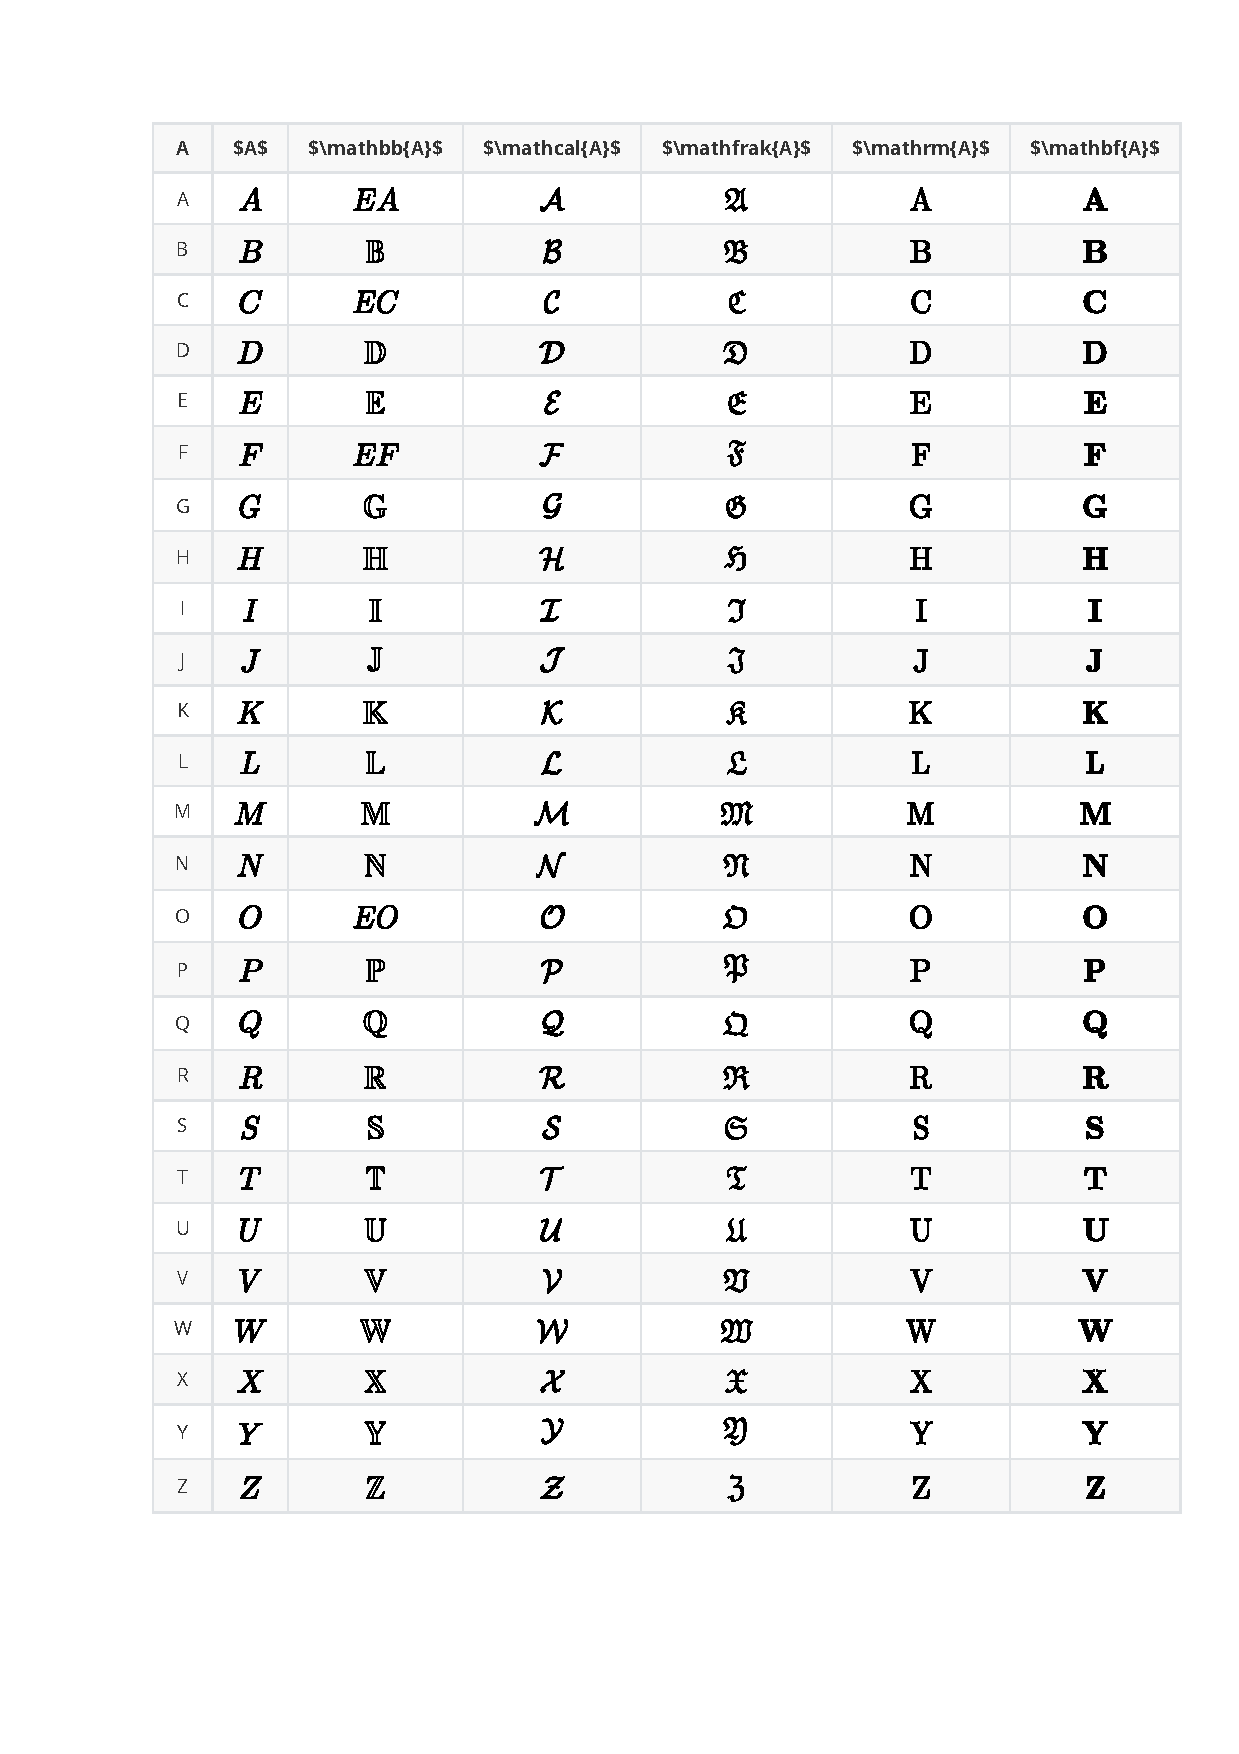
\includepdf{mathfonts.pdf}

\subsection{\LaTeX 中的颜色}
参考\href{http://latexcolor.com/}{latexcolor}。

\subsection{注脚}
两种常用形式:
\begin{itemize}
	\item \begin{verbatim}\footnote{注脚的内容}\end{verbatim}
	\item 这种方式很方便,可以在多处共享一个注脚,只需使用同一个注脚编号即可
	\begin{verbatim}
		\footnotemark[注脚编号]
		\footnotetext[编号]{注脚内容}
	\end{verbatim}
\end{itemize}

\subsection{章节编号}
默认是从1开始编号的,如果要从0开始,可以加一条命令:\begin{verbatim}\setcounter{section}{-1}\end{verbatim}










\section{Datasets}
\subsection{MovieLens 100K}


\clearpage
\part{BigData}
{\noindent}	 \rule[-10pt]{17.5cm}{0.5em}\\

\section{HDFS}
存储在 HDFS 中的文件是如何被 MapReduce 处理的?存储在 HDFS 中的文件会被分为一个一个的块 (block) , 分散存储在 datanode 中. 注意此处的快并不是磁盘中的数据块, 磁盘中的数据块是磁盘进行读写的最小单位, 磁盘的块大小一般是几百字节. 文件系统是构建在磁盘之上的 (可以构建于一块磁盘, 也可以构建于多块磁盘) , 文件系统 (FS) 中也存在块的概念, 通常 FS 中的块大小是磁盘块的倍数, FS 通过文件系统的块来管理磁盘, 存储在一个文件系统中的文件会被分成多个文件系统的块来存储. HDFS 作为一个分布式的文件系统, 其实也是一个文件系统, 因此其也有块的概念. HDFS 中的块一般是 128MB. 一个文件存储进 HDFS 时会被分成多个 block, block 就是 HDFS 的存储单元. InputSplit 是一个逻辑概念, 并没有对实际文件进行切分, 它只包含一些元数据信息, 比如数据的起始位置, 数据长度, 数据所在的节点等. 它的划分方法完全取决于用户自己. 但是需要注意的是 InputSplit 的多少决定了 Map Task 的数目, 因为每个 InputSplit 会交由一个 Map Task 处理. 当MapReduce作业客户端计算 InputSplit 时, 它会计算出块中第一个记录的开始位置和最后一个记录的结束位置. 在最后一个记录不完整的情况下, InputSplit 包括下一个块的位置信息和完成该记录所需的数据的字节偏移. 

\section{MapReduce}
一个 MR job 通常会把输入数据划分成独立的 chunks. 每个 chunk 会被 map tasks 并行地处理. 然后 MR 这个框架会对 map 的输出进行排序, 然后输入给 reduce tasks. 通常输入和输出都存储在文件系统中. tasks 的调度由 MR 框架负责, 监控它们的执行并再执行失败的任务. MR 框架中有一个 ResourceManager, 每个 worker 节点一个 NodeManager, 每个应用一个 MRAppMaster. 最低程度上,一个 MR 应用等于: 输入/输出 + map 和 reduce 函数(实现了相应的接口)+ 关于 job 的一些参数 (job configuration). 有了 job 后, Hadoop 的 job-client 会提交 job (即可执行文件) 以及配置给 ResourceManager, 它会把这些\textbf{可执行文件}和\textbf{配置}分发到各个 workers, 调度和监控 tasks 的执行并把状态数据发送给 job-client.

\subsection{一些基本概念}

\par{\textbf{\textcolor{red}{Mapper}}}$\quad$ 对于 InputFormat 生成的每个 InputSplit, MR 都会产生一个对应的 map task 进行处理. map 输入输出的类型和数量不一定要相同. 对于 mapper 输出的 k-v pairs. 并不是直接输入给 reducer, 而是会由框架进行一次处理后在输入给 reducer. 处理的方式: 按照 key 对输出进行聚合. Mapper 任务的输出还会再进行一次排序然后进行划分, 每个 reducer 一个 partition. 如果没有 Reducer, 则 mapper 的输出会直接写道文件系统中, 此时则不会对输出进行排序. 

\par{\textbf{\textcolor{red}{Reducer}}}$\quad$ Reducer 主要分成三成三个阶段: shuffle, sort 和 reduce. Reducer 的输出一般会写到文件系统中. 在真的执行 reduce 函数时, 会对 pair 进行聚合, 得到 <key, list of values> 这样的 pair, reduce 函数实际的输入就是这样的 pair. 

\par{\textbf{\textcolor{red}{Combiner}}}$\quad$ 对 Mapper 输出的数据进行规约处理, 减小传送到reduce端的数据量, 缩短传输时间和作业的整体时间. Combiner 是在 Mapper 任务内完成的, 不能跨 Mapper, 但 Reducer可以接收多个 Mapper 的输出.

\par{\textbf{\textcolor{red}{InputFormat}}}$\quad$ MR 程序获取的数据类型多种多样, 当程序把数据输入给 Mapper 时, 需要格式化读取, 例如读取普通文本文件使用 TextInputFormat. 所有的输入格式类都继承于 InputFormat, 它的主要作用是将输入数据切分成分片 (比如多少行为一个分片,即 InputSplit), 以及如何读取分片中的数据 (比如按行读取), 前者由 getSplits() 完成, 后者由 RecordReader 完成.

\subsection{Shuffle 机制}
只闻 map 与 reduce, 未闻 shuffle 显神功. 

\textbf{shuffle 是 MR 大数据处理中的一个阶段: 从 map 处理完到 reduce 的输入}. 为什么要有 shuffle 呢?

map 输出的每个 <k, v> pair, MR 都会为其计算一个 partition 值 ($=hash(k) \% num\_reduce\_task$). map task 执行时是迭代的地读取 record 的, 当生成的数据过多的时则会 spill 到磁盘, 即生成文件, 处理的过程中可能会 spill 多次, 因此可能会有多个小文件. 每个文件包含了各个分区的数据, 因此需要一个 merge 的过程: 将不同文件中同一分区的数据聚合, 并在分区内对数据进行排序.

所有的 map tasks 结束后才会开始 Reduce Task, reduce task 并不是立刻就对数据进行计算的. 注意到 map task, reduce task 可能分布在不同的计算节点上, 因此在真正开始执行猿编写的 reducer 之前还有一些操作, 即在 reduce 端的 shuffle. 是的, 从 map 的输出到 reduce 的输入这段时间都由 shuffle 来负责. 每个 reduce task 处理一个分区, 其输入数据可能来自任何一个 map task 的输出. 因此对一个 reduce task 来说, 其会从各个 map task 中拉取 (通过 http 协议) 对应的分区的数据. 由于来自各个 map task 的数据是分散的, 因此还需要将这些数据进行 merge 并进行排序, 然后再输入给 reducer 进行处理. 至此, shuffle 的工作就结束了. 

\begin{figure}[h]
	\centering
	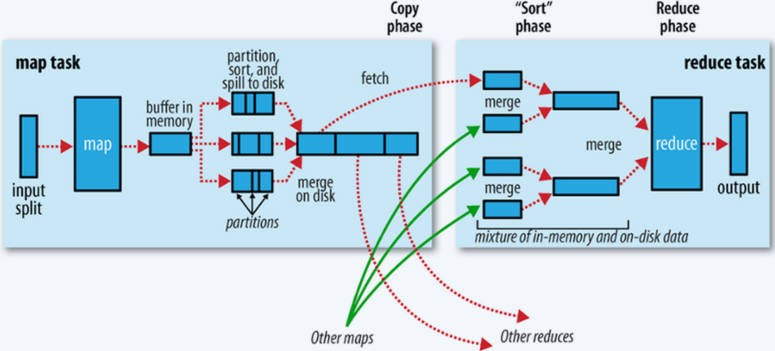
\includegraphics[width=.95\textwidth]{pics/mr_shuffle.jpg}
	\caption{Shuffle}
	\label{fig:mr-shuffle}
\end{figure}

通过以上简单的介绍, 其实已经体现了 shuffle 的作用: 1) 处理 mapper 的输出, 按照分区进行 merge; 2) 从 map 结点获取数据并 merge 作为 reduce 的输入; 3) shuffle 为猿们处理了这一繁杂的过程, 其中涉及到很多细节, 如内存中缓冲的数据如何 spill 到磁盘中, spill 文件的格式, reduce 如何拉取对应的数据等.

以上只是一个简单的介绍, 其实还有很多细节.

\section{Spark}
老早就久仰 Spark 的大名, 自己也在服务器上用 docker 搭过 Spark 集群, 做了一点简单的尝试, 但总是差点感觉, 处于盲人摸象的阶段, 对 Spark 的认识还是一团浆糊. 有幸接触到了 《大数据处理框架 Apache Spark 设计与实现》\footnote{许利杰, 方亚芬著, 电子工业出版社}, 解答了我不少困惑. 

众所周知, Spark 是一个分布式计算框架, 于 2012 年由 UC Berkeley 的 AMPLab 研发并开源. 其核心思想包括两方面: 
\begin{itemize}
	\item 对大数据处理框架的输入/输出, 中间数据进行建模, 将这些数据抽象为统一的数据结构 (RDD, 最新版的 Spark 增加了 Dataset, DataFram 等高层 API), 并在此数据结构的基础上构建了一系列通用的数据操作;
	
	\item 采用基于内存的数据聚合, 数据缓存机制加速应用的执行.
\end{itemize}

多年的发展, Spark 也发展出了自己的生态, 以 Spark 处理框架为核心, 在上层构建了面向 SQL 的 Spark SQL 框架, 面向大规模图计算的 GraphX 框架, 面向大规模机器学习的 MLlib 框架及算法库, 以及面向流处理的 Spark Streaming 框架; 在下层,  也推出了相关的存储系统, 如基于分布式文件系统的 Alluxio, 支持 ACID 事务的数据湖系统 Delta Lake 等. 


\subsection{Overview}

Spark 处理的核心: \textcolor{red}{\textbf{如何将应用程序转化为可以分布式执行的计算任务?}}

从一个 Spark Application 开始. 
\begin{itemize}
	\item 一个 Spark 应用包含了用户代码, 配置, 以及要处理的数据 (可以是存储在分布式文件系统, 数据库中的数据, 也可以是流式数据等);
	
	\item 那要怎么执行一个 Spark 应用呢? Spark 作为一个分布式计算框架, 是可以部署在多个结点上的, Spark 采用的是主从式的结构, 系统架构中包含了一个 Master 结点和多个 Worker 结点: Master 负责管理应用和任务, Worker 负责执行任务. 当我们要在 Spark 集群上执行一个应用时, 需要将应用 (及代码, 配置, 数据) 提交到集群上 --- 具体是通过什么提交和提交到哪呢? 通过什么提交, 这个问题等价于 --- 当 Spark 集群部署好之后, 怎么与集群交互. 部署完后, Spark 集群就相当于服务的提供方 --- Sever, 而我们则可以通过 Client 与 Server 进行交互. Client 具体是什么样子的, 取决于 Spark 集群的部署模式, 主要有: Standalone, Mesos, YARN, Kubernetes. 先不管不同部署模式的区别, 它们都会为我们提供一个与集群交互的入口, 通过这个入口我们可以向集群提交应用 (当然也可以干别的, 比如启动和关闭集群);
	
	\item 提交应用后, 集群中的 Master 结点会接收应用. 和普通的程序有一个入口 (\textit{main()} 函数) 一样, Spark 应用在执行时也有一个入口. Master 收到一个用后会启动一个 Driver (官方的解释: "The process running the main() function of the application and creating the SparkContext") 进程, 用于运行应用的 \textit{main()} 函数. Driver 的作用包括: 与集群管理者进行交互, 对应用进行划分, 管理 Worker 上相关任务的执行. Master 也会为应用在 Worker 上分配计算资源 --- Executor 进程. Executor 进程中会有多个线程用于执行其负责的计算任务 (即 Task). 
	
	\item 资源差不多分配妥当后, Driver 会对应用进行分解, 怎么分解呢? 一个 Spark 应用程序包含了对数据的处理流程, 一个应用对应着多个 job, 每个 job 由多个 stage 组成, 每个 stage 可以拆分成多个 task. Driver 会将 task 分发给 Worker, 由 Executor 中的线程完成 task. 
	
	\item 计算完成后可以将结果汇集到 Driver 端, 或者保存至磁盘中.
\end{itemize}

上面涉及到的一些概念:

\begin{itemize}
	\item Master 进程. 运行在 Master 结点上, 该进程负责管理全部的 Worker 结点, 监控 Worker 结点的存活状态;
	
	\item Worker 进程. 运行在 Worker 结点上, 该进程除了与 Master 结点通信, 还负责管理任务的执行, 监控任务执行的状态;
\end{itemize}
 
\subsection{逻辑处理流程}

Spark 应用的逻辑处理流程指应用的计算过程在 Spark 内部的表示, 主要包括四部分:

\begin{itemize}
	\item 数据源. 即原始数据, 可以存放在本地文件系统, 分布式文件系统, 或者来自网络流等;
	
	\item 数据模型. 即输入 / 输出, 中间数据在 Spark 内的表示, 其中最基础的一个便是 RDD (Resilient Distributed Datasets), 其可以包含多个数据分区, 不同数据分区可以由不同的任务在不同节点处理;
	
	\item 数据操作. 即 Spark 中对 RDD 的各种操作, 分为两种: \textit{transformation, action}. action 类的操作会触发 Spark 提交 job 真正执行数据处理任务. transformation 类的操作是单向的, 即 RDD 进行 transformation 后会生成新的 RDD, 而不是对 RDD 本身进行修改;
	
	\item 计算结果处理. 由于 RDD 是分布在不同机器上的, 应用的结果计算方式分为两种: 1) 直接将计算结果保存到分布式文件系统中; 2) 将计算结果汇集到 Driver 端进行集中计算. 
\end{itemize}

逻辑处理流程等价于计算过程中涉及到的 RDD 及其之间的依赖关系. 除了输入数据转化成的 RDD, Spark 中的数据操作也会生出 RDD, 不同的操作会产生不同的依赖关系, 但总的可以分为两大类: 窄依赖和宽依赖. 

\begin{figure}[h]
	\centering
	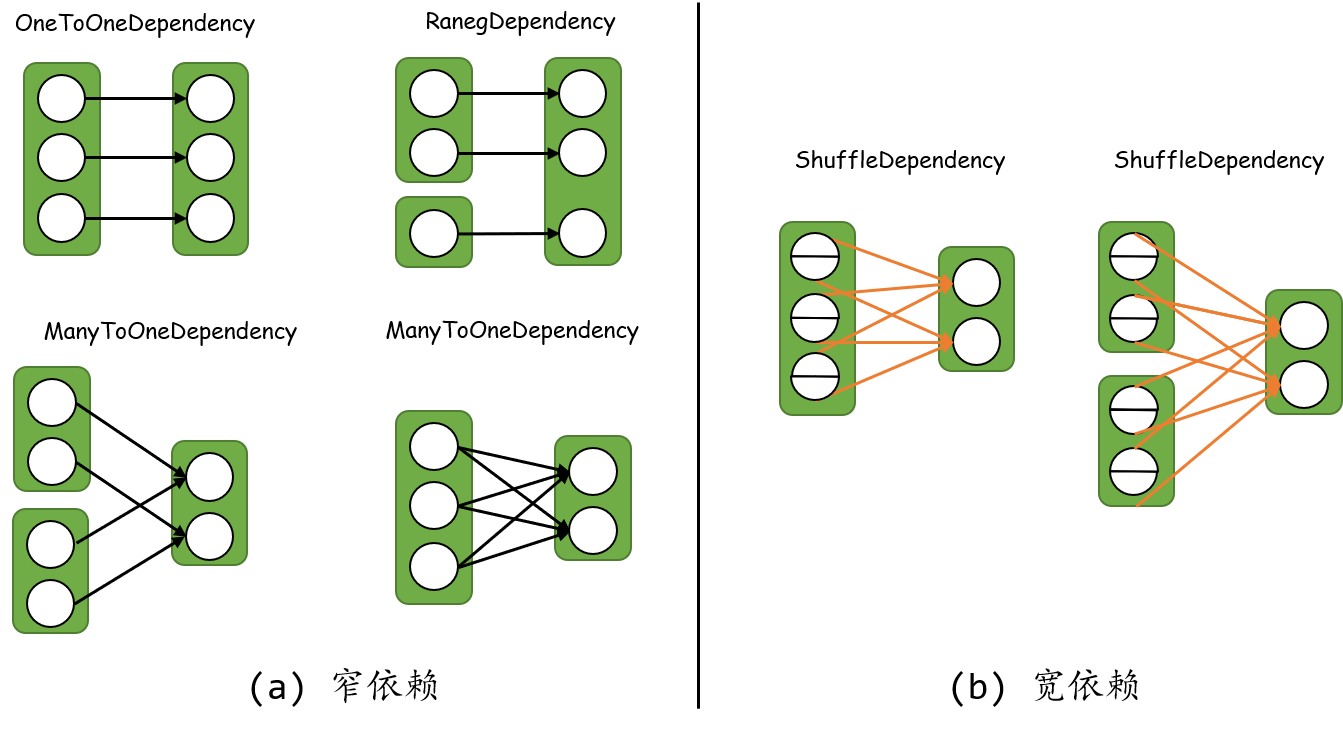
\includegraphics[width=.95\textwidth]{pics/RDD-Dependency.png}
	\caption{RDD 中的依赖关系}
	\label{fig:rdd_den}
\end{figure}

\subsubsection{窄依赖}

子 RDD 中每个分区都依赖于父 RDD 中的一部分分区, 如 Fig.\ref{fig:rdd_den}(a) 所示. 可以分成四种窄依赖:

\begin{itemize}
	\item 一对一依赖 (OneToOneDependency). 子 RDD 和父 RDD 的分区个数相同, 且存在一一映射关系, 典型的 transformation 包括 \textit{map(), filter()};
	
	\item 区域依赖 (RangeDependency). 子 RDD 和父 RDD 的分区经过区域化后存在一一映射关系, 如 \textit{union()};
	
	\item 多对一依赖 (ManyToOneDependency). 子 RDD 中的一个分区依赖\textbf{多个父 RDD} 中的分区, 如 \textit{join()};
	
	\item 多对多依赖 (ManyToManyDependency). 子 RDD 中的一个分区依赖父 RDD 中的多个分区, 同时发父 RDD 中的一个分区被子 RDD 中的多个分区依赖, 如 \textit{cartesian()}.
\end{itemize}

ManyToOneDependency 和 ManyToManyDependency 是我参考《大数据处理框架 Apache Spark 设计与实现》引入的, 实际在 Spark 代码中并没有对这两种依赖进行命名.

\subsubsection{宽依赖}

子 RDD 中的分区依赖父 RDD 中每个分区的一部分, 如 Fig.\ref{fig:rdd_den}(b) 所示. 典型的宽依赖 transformation 包括 \textit{groupByKey(), partitionBy(), reduceByKey()} 等.

窄, 宽依赖的区别在于子 RDD 的各个分区是否\textbf{完全依赖} (\textcolor{red}{指父 RDD 中的一个分区不需要进行划分就可以流入子 RDD 的分区中})父 RDD 的一个或多个分区. 

\textcolor{red}{为什么要进行数据以来关系进行分类呢?} 1) 明确 RDD 分区之间的数据依赖关系, 执行时可以确定从哪里获得数据, 输出数据到哪; 2) 有利于生成物理执行计划. 同一 stage 内的窄依赖的分区可以并行执行, 宽依赖需要进行 Shuffle. 

\subsubsection{数据分区方法}

RDD 内部的数据是如何分区的. Spark 中的分区方法:

\begin{itemize}
	\item 水平划分. 按照 record 的索引进行划分;
	
	\item Hash 划分 (HashPartitioner). 使用 record 的 Hash 值对数据进行划分;
	
	\item Range 划分 (RangePartitioner). 按照元素的序关系进行划分;
	
	\item 自定义划分. 按照自己的需求实现 Partitioner.
\end{itemize}



\subsection{物理执行计划}

有了逻辑执行计划 (即 RDD 组成的数据依赖有向无环图), 该怎么去执行呢? 物理执行计划即 Spark 是如何完成计算的. Spark 以逻辑执行计划为基础生成物理执行计划. 

\subsection{Shuffle 机制}


\clearpage
\part{Others}
{\noindent}	 \rule[-10pt]{17.5cm}{0.5em}\\
\section{Others}
\subsection{李沐 --- 用随机梯度下降来优化人生}
\textbf{要有目标}。你需要有目标。短的也好,长的也好。认真定下来的也好,别人那里捡来的也好。就跟随机梯度下降需要有个目标函数一样。

\textbf{目标要大}。不管是人生目标还是目标函数,你最好不要知道最后可以走到哪里。如果你知道,那么你的目标就太简单了,可能是个凸函数。你可以在一开始的时候给自己一些小目标,例如期末考个80分,训练一个线性模型。但接下来得有个更大的目标,财富自由也好,100亿参数的变形金刚也好,得足够一颗赛艇。

\textbf{坚持走}。不管你的目标多复杂,随机梯度下降都是最简单的。每一次你找一个大概还行的方向(梯度),然后迈一步(下降)。两个核心要素是方向和步子的长短。但最重要的是你得一直走下去,能多走几步就多走几步。

\textbf{痛苦的卷}。每一步里你都在试图改变你自己或者你的模型参数。改变带来的痛苦。但没有改变就没有进步。你过得很痛苦不代表在朝着目标走,因为你可能走反了。但是过得很舒服那一定在原地踏步。需要时刻跟自己作对。

\textbf{可以躺平}。你用你内心的激情来迈步子。步子太小走不动,步子太长容易过早消耗了激情。周期性的调大调小步长效果挺好。所以你可以时不时休息休息。

\textbf{四处看看}。每一步走的方向是你对世界的认识。如果你探索的世界不怎么变化,那么要么你的目标太简单,要么你困在你的舒适区了。随机梯度下降的第一个词是随机,就是你需要四处走走,看过很多地方,做些错误的决定,这样你可以在前期迈过一些不是很好的舒适区。

\textbf{快也是慢}。你没有必要特意去追求找到最好的方向和最合适的步子。你身边当然会有幸运之子,他们每一步都在别人前面。但经验告诉我们,随机梯度下降前期进度太快,后期可能乏力。就是说你过早的找到一个舒适区,忘了世界有多大。所以你不要太急,前面徘徊一段时间不是坏事。成名无需太早。

\textbf{赢在起点}。起点当然很重要。如果你在终点附近起步,可以少走很多路。而且终点附近的路都比较平,走着舒服。当你发现别人不如你的时候,看看自己站在哪里。可能你就是运气很好,赢在了起跑线。如果你跟别人在同一起跑线,不见得你能做更好。

\textbf{很远也能到达}。如果你是在随机起点,那么做好准备面前的路会非常不平坦。越远离终点,越人迹罕至。四处都是悬崖。但随机梯度下降告诉我们,不管起点在哪里,最后得到的解都差不多。当然这个前提是你得一直按照梯度方向走下去。如果中间梯度炸掉了,那么你随机一个起点,调整步子节奏,重新来。

\textbf{独一无二}。也许大家有着差不多的目标,在差不多的时间毕业买房结婚生娃。但每一步里,每个人的内心中看到的世界都不一样,导致走的路不一样。你如果跑多次随机梯度下降,在各个时间点的目标函数值可能都差不多,但每次的参数千差万别。不会有人关心你每次训练出来的模型里面参数具体是什么值,除了你自己。

\textbf{简单最好}。当然有比随机梯度下降更复杂的算法。他们想每一步看向更远更准,想步子迈最大。但如果你的目标很复杂,简单的随机梯度下降反而效果最好。深度学习里大家都用它。关注前面,每次抬头瞄一眼世界,快速做个决定,然后迈一小步。小步快跑。只要你有目标,不要停,就能到达。


% %一 \section{Task description and data construction}
% \label{sec:headings}

%\subsection{Headings: second level}
% \begin{equation}
% \xi _{ij}(t)=P(x_{t}=i,x_{t+1}=j|y,v,w;\theta)= {\frac {\alpha _{i}(t)a^{w_t}_{ij}\beta _{j}(t+1)b^{v_{t+1}}_{j}(y_{t+1})}{\sum _{i=1}^{N} \sum _{j=1}^{N} \alpha _{i}(t)a^{w_t}_{ij}\beta _{j}(t+1)b^{v_{t+1}}_{j}(y_{t+1})}}
% \end{equation}



% \section{Examples of citations, figures, tables, references}
% The documentation for \verb+natbib+ may be found at
% \begin{center}
%   \url{http://mirrors.ctan.org/macros/latex/contrib/natbib/natnotes.pdf}
% \end{center}


% \begin{verbatim}
%   \citet{hasselmo} investigated\dots
% \end{verbatim}

% \begin{quote}
%   Hasselmo, et al.\ (1995) investigated\dots
% \end{quote}

% \begin{center}
%   \url{https://www.ctan.org/pkg/booktabs}
% \end{center}

% 引用表格
% 需要给表格加上标签, 格式: \label{fig:fig1}
% \ref{fig:fig1}

% \subsection{Figures}
% 123123
% See Figure \ref{fig:fig1}. Here is how you add footnotes. \footnote{Sample of the first footnote.}
% 123123

% \begin{figure}
%   \centering
%   \fbox{\rule[-.5cm]{4cm}{4cm} \rule[-.5cm]{4cm}{0cm}}
%   \caption{Sample figure caption.}
%   \label{fig:fig1}
% \end{figure}


% 表格
% \subsection{Tables}
% 1312
% See awesome Table~\ref{tab:table}.

% \begin{table}
%  \caption{Sample table title}
%   \centering
%   \begin{tabular}{lll}
%     \toprule
%     \multicolumn{2}{c}{Part}                   \\
%     \cmidrule(r){1-2}
%     Name     & Description     & Size ($\mu$m) \\
%     \midrule
%     Dendrite & Input terminal  & $\sim$100     \\
%     Axon     & Output terminal & $\sim$10      \\
%     Soma     & Cell body       & up to $10^6$  \\
%     \bottomrule
%   \end{tabular}
%   \label{tab:table}
% \end{table}



% 打印参考文献
\printbibliography
\bibliographystyle{plain}
\bibliography{references}



\end{document}
